% Template:     Informe/Reporte LaTeX
% Documento:    Archivo principal
% Versión:      6.2.2 (30/01/2019)
% Codificación: UTF-8
%
% Autor: Pablo Pizarro R. @ppizarror
%        Facultad de Ciencias Físicas y Matemáticas
%        Universidad de Chile
%        pablo.pizarro@ing.uchile.cl, ppizarror.com
%
% Manual template: [https://latex.ppizarror.com/Template-Informe/]
% Licencia MIT:    [https://opensource.org/licenses/MIT/]

% CREACIÓN DEL DOCUMENTO
\documentclass[letterpaper,11pt]{article} % Articulo tamaño carta, 11pt
\usepackage[utf8]{inputenc} % Codificación UTF-8

% INFORMACIÓN DEL DOCUMENTO
\def\titulodelinforme {Apunte}
\def\temaatratar {Reactores Químicos y Bioquímicos}

\def\autordeldocumento {Juan Saez Hidalgo}
\def\nombredelcurso {Reactores Químicos y Bioquímicos}
\def\codigodelcurso {IQ4305}

\def\nombreuniversidad {Universidad de Chile}
\def\nombrefacultad {Facultad de Ciencias Físicas y Matemáticas}
\def\departamentouniversidad {Departamento de Ing Química, Biotecnología y Materiales}
\def\imagendepartamento {(departamentos/fcfm}
\def\imagendepartamentoescala {0.1}
\def\localizacionuniversidad {Santiago, Chile}

% INTEGRANTES, PROFESORES Y FECHAS
\def\tablaintegrantes {
\begin{tabular}{ll}
	Alumno:
	& \begin{tabular}[t]{l}
		Juan Saez Hidalgo
	\end{tabular} \\
	Carrera:
	& \begin{tabular}[t]{l}
		Licenciatura en Ciencias de la Ingeniería \\
		mención Biotecnología
	\end{tabular} \\
	Email:
	& \begin{tabular}[t]{l}
		juan.saez.h@ing.uchile.cl
	\end{tabular} \\
	\multicolumn{2}{r}{\localizacionuniversidad}
\end{tabular}}{
}

% CONFIGURACIONES
% Template:     Informe/Reporte LaTeX
% Documento:    Configuraciones del template
% Versión:      6.2.2 (30/01/2019)
% Codificación: UTF-8
%
% Autor: Pablo Pizarro R. @ppizarror
%        Facultad de Ciencias Físicas y Matemáticas
%        Universidad de Chile
%        pablo.pizarro@ing.uchile.cl, ppizarror.com
%
% Manual template: [https://latex.ppizarror.com/Template-Informe/]
% Licencia MIT:    [https://opensource.org/licenses/MIT/]

% CONFIGURACIONES GENERALES
\def\addemptypagetwosides {false}  % Añade pag en blanco al imprimir a 2 caras
\def\defaultinterline {1.2}        % Interlineado por defecto [pt]
\def\defaultnewlinesize {11}       % Tamaño del salto de línea [pt]
\def\documentlang {es-CL}          % Define el idioma del documento
\def\fontdocument {lmodern}        % Tipografía base, ver soportadas en manual
\def\fonttypewriter {tmodern}      % Tipografía de \texttt, ver manual online
\def\importtikz {false}            % Utilizar la librería tikz
\def\pointdecimal {true}           % N° decimales con punto en vez de coma
\def\predocuseromannumber {true}   % Pág. con número romano previo a inicio doc.
\def\romanpageuppercase {false}    % Páginas en número romano en mayúsculas
\def\showlinenumbers {false}       % Muestra los números de línea del documento

% ESTILO PORTADA Y HEADER-FOOTER
\def\hfstyle {style1}              % Estilo header-footer (14 estilos)
\def\portraitstyle {style6}        % Estilo portada (18 estilos)

% CONFIGURACIÓN DE LAS LEYENDAS - CAPTION
\def\captionalignment {justified}  % Posición {centered,justified,left,right}
\def\captionlabelformat {simple}   % Formato leyenda {empty,simple,parens}
\def\captionlabelsep {colon}       % Sep. {none,colon,period,space,quad,newline}
\def\captionlessmarginimage {0.1}  % Margen sup/inf de fig. si no hay ley. [cm]
\def\captionlrmargin {0.6}         % Márgenes izq/der de la leyenda [cm]
\def\captionmarginmultimg {0.45}   % Margen izq/der leyendas múltiple img [cm]
\def\captionnumcode {arabic}       % N° código {arabic,alph,Alph,roman,Roman}
\def\captionnumfigure {arabic}     % N° figuras {arabic,alph,Alph,roman,Roman}
\def\captionnumsubfigure {alph}    % N° subfiguras {arabic,alph,Alph,roman,Roman}
\def\captionnumsubtable {alph}     % N° subtabla {arabic,alph,Alph,roman,Roman}
\def\captionnumtable {arabic}      % N° tabla {arabic,alph,Alph,roman,Roman}
\def\captiontbmarginfigure {9.35}  % Margen sup/inf de la leyenda en fig. [pt]
\def\captiontbmargintable {7.0}    % Margen sup/inf de la leyenda en tab. [pt]
\def\captiontextbold {false}       % Etiqueta (código,figura,tabla) en negrita
\def\codecaptiontop {true}         % Leyenda arriba del código fuente
\def\figurecaptiontop {false}      % Leyenda arriba de las imágenes
\def\showsectioncaption {none}     % N° sec. en objeto {none,(s/ss/sss/ssss)ec}
\def\subcaptionlabelformat{parens} % Formato leyenda sub. {empty,simple,parens}
\def\subcaptionlabelsep {space}    % Sep. {none,colon,period,space,quad,newline}
\def\tablecaptiontop {true}        % Leyenda arriba de las tablas

% CONFIGURACIÓN DEL ÍNDICE
\def\charafterobjectindex {.}      % Carácter después de n° figura,tabla,código
\def\charnumpageindex {.}          % Carácter número de página en índice
\def\equalmarginnumobject {true}   % Iguala el margen de los números de objetos
\def\indexdepth {4}                % Profundidad máxima del índice
\def\indexnewpagec {false}         % Nueva página en índice códigos fuente
\def\indexnewpagef {false}         % Nueva página en índice figuras
\def\indexnewpaget {false}         % Nueva página en índice tablas
\def\indexstyle {ftc}              % Estilo índice: f:figura, t:tabla, c:código
\def\indextitlemargin {11.4}       % Margen título índice \insertindextitle [pt]
\def\objectindexindent {true}      % Indenta la lista de objetos
\def\resetpagnumafterindex {true}  % Resetea número de la pag. tras el índice
\def\showindex {true}              % Muestra el índice
\def\showindexofcontents {true}    % Muestra la lista de contenidos

% ANEXO, CITAS, REFERENCIAS
\def\apaciterefsep {9}             % Separación entre refs. {apacite} [pt]
\def\appendixindepobjnum {true}    % Anexo usa n° objetos independientes
\def\bibtexrefsep {9}              % Separación entre refs. {bibtex} [pt]
\def\natbibrefsep {5}              % Separación entre referencia {natbib} [pt]
\def\natbibrefstyle {apa}       % Formato de ref. natbib {apa,ieeetr,etc..}
\def\sectionappendixlastchar {.}   % Carácter entre n° de sec. anexo y título
\def\sectionrefenv {true}         % Las referencias se consideran como sección
\def\showappendixsecindex {false}  % Título de la sec. de anexos en el índice
\def\stylecitereferences {apacite}  % Estilo cita/ref. {apacite,bibtex,natbib}
\def\twocolumnreferences {false}   % Referencias en dos columnas

% CONFIGURACIONES DE OBJETOS
\def\columnhspace {-0.4}           % Margen horizontal entre obj. \createcolumn
\def\columnsepwidth {0.6}          % Separación entre columnas [em]
\def\defaultimagefolder {img/}     % Carpeta raíz de las imágenes
\def\equationrestart {none}         % N° ecuación {none,page,(s/ss/sss/ssss)ec}
\def\footnoterestart {none}        % N° footnote {none,page,(s/ss/sss/ssss)ec}
\def\imagedefaultplacement {H}     % Posición por defecto de las imágenes
\def\marginalignbottom {-0.30}     % Margen inferior entorno align [cm]
\def\marginaligncaptbottom {0.05}  % Margen inferior entorno align caption[cm]
\def\marginaligncapttop {-0.60}    % Margen superior entorno align caption [cm]
\def\marginaligntop {-0.40}        % Margen superior entorno align [cm]
\def\marginalignedbottom {-0.30}   % Margen inferior entorno aligned [cm]
\def\marginalignedcaptbottom {0.0} % Margen inferior entorno aligned caption[cm]
\def\marginalignedcapttop {-0.60}  % Margen superior entorno aligned caption [cm]
\def\marginalignedtop {-0.40}      % Margen superior entorno aligned [cm]
\def\margineqncaptionbottom {0.0}  % Margen inferior caption ecuación [cm]
\def\margineqncaptiontop {-0.65}   % Margen superior caption ecuación [cm]
\def\marginequationbottom {-0.15}  % Margen inferior ecuaciones [cm]
\def\marginequationtop {0.0}       % Margen superior ecuaciones [cm]
\def\marginfloatimages {-13.0}     % Margen sup. fig. \insertimageleft/right [pt]
\def\marginfootnote {10.0}         % Margen derecho footnote [pt]
\def\margingatherbottom {-0.20}    % Margen inferior entorno gather [cm]
\def\margingathercaptbottom {0.05} % Margen inferior entorno gather caption [cm]
\def\margingathercapttop {-0.77}   % Margen superior entorno gather [cm]
\def\margingathertop {-0.40}       % Margen superior entorno gather [cm]
\def\margingatheredbottom {-0.10}  % Margen inf. entorno gathered [cm]
\def\margingatheredcaptbottom{0.0} % Margen inf. entorno gathered caption [cm]
\def\margingatheredcapttop {-0.77} % Margen superior entorno gathered [cm]
\def\margingatheredtop {-0.40}     % Margen superior entorno gathered [cm]
\def\marginimagebottom {-0.15}     % Margen inferior figura [cm]
\def\marginimagemultright {0.50}   % Margen derecho imágenes múltiples [cm]
\def\marginimagemulttop {-0.30}    % Margen superior imágenes múltiples [cm]
\def\marginimagetop {0.0}          % Margen superior figuras [cm]
\def\numberedequation {true}       % Ecuaciones con \insert... numeradas
\def\tabledefaultplacement {H}     % Posición por defecto de las tablas
\def\tablepaddingh {1.0}           % Espaciado horizontal de celda de las tablas
\def\tablepaddingv {1.0}           % Espaciado vertical de celda de las tablas
\def\tikzdefaultplacement {H}      % Posición por defecto de las figuras tikz

% CONFIGURACIÓN DE LOS TÍTULOS
\def\anumsecaddtocounter {false}   % Insertar títulos 'anum' aumenta n° de sec
\def\disablehfrightmark {false}    % Desactiva el rightmark del header-footer
\def\fontsizessstitle{\normalsize} % Tamaño sub-sub-subtítulos
\def\fontsizesubsubtitle {\large}  % Tamaño sub-subtítulos
\def\fontsizesubtitle {\Large}     % Tamaño subtítulos
\def\fontsizetitle {\LARGE}        % Tamaño títulos
\def\fontsizetitlei {\LARGE}       % Tamaño títulos en el índice
\def\showdotaftersnum {true}       % Punto al final de n° (s/ss/sss/ssss)ection
\def\stylessstitle {\bfseries}     % Estilo sub-sub-subtítulos
\def\stylesubsubtitle {\bfseries}  % Estilo sub-subtítulos
\def\stylesubtitle {\bfseries}     % Estilo subtítulos
\def\styletitle {\bfseries}        % Estilo títulos
\def\styletitlei {\bfseries}       % Estilo títulos en el índice

% CONFIGURACIÓN DE LOS COLORES DEL DOCUMENTO
\def\captioncolor {black}          % Color de la leyenda (código,figura,tabla)
\def\captiontextcolor {black}      % Color de la leyenda
\def\colorpage {white}             % Color de la página
\def\highlightcolor {yellow}       % Color del subrayado con \hl
\def\indextitlecolor {black}       % Color de los títulos del índice
\def\linenumbercolor {gray}        % Color del n° de línea (\showlinenumbers)
\def\linkcolor {black}             % Color de los links del documento
\def\maintextcolor {black}         % Color principal del texto
\def\numcitecolor {black}          % Color del n° de las referencias o citas
\def\portraittitlecolor {black}    % Color de los títulos de la portada
\def\showborderonlinks {false}     % Color de un link por un recuadro de color
\def\sourcecodebgcolor {lgray}     % Color de fondo del código fuente
\def\ssstitlecolor {black}         % Color de los sub-sub-subtítulos
\def\subsubtitlecolor {black}      % Color de los sub-subtítulos
\def\subtitlecolor {black}         % Color de los subtítulos
\def\tablelinecolor {black}        % Color de las líneas de las tablas
\def\titlecolor {black}            % Color de los títulos
\def\urlcolor {blue}               % Color de los enlaces web (\href,\url)

% MÁRGENES DE PÁGINA
\def\firstpagemargintop {3.8}      % Margen superior página portada [cm]
\def\pagemarginbottom {2.7}        % Margen inferior página [cm]
\def\pagemarginleft {2.54}         % Margen izquierdo página [cm]
\def\pagemarginright {2.54}        % Margen derecho página [cm]
\def\pagemargintop {3.0}           % Margen superior página [cm]

% OPCIONES DEL PDF COMPILADO
\def\addindextobookmarks {false}   % Añade el índice a los marcadores del pdf
\def\cfgbookmarksopenlevel {1}     % Nivel marcadores en pdf (1:secciones)
\def\cfgpdfbookmarkopen {true}     % Expande marcadores del nivel configurado
\def\cfgpdfcenterwindow {true}     % Centra ventana del lector al abrir el pdf
\def\cfgpdfcopyright {}            % Establece el copyright del documento
\def\cfgpdfdisplaydoctitle {true}  % Muestra título del informe en visor
\def\cfgpdffitwindow {false}       % Ajusta la ventana del lector tamaño pdf
\def\cfgpdfmenubar {true}          % Muestra el menú del lector
\def\cfgpdfpagemode {OneColumn}    % Modo de página {OneColumn,SinglePage}
\def\cfgpdfpageview {FitH}         % {Fit,FitH,FitV,FitR,FitB,FitBH,FitBV}
\def\cfgpdfsecnumbookmarks {true}  % Número de la sec. en marcadores del pdf
\def\cfgpdftoolbar {true}          % Muestra barra de herramientas lector pdf
\def\cfgshowbookmarkmenu {false}   % Muestra menú marcadores al abrir el pdf
\def\pdfcompileversion {7}         % Versión mínima del pdf compilado (1.x)

% NOMBRE DE OBJETOS
\def\nameabstract {Resumen}           % Nombre del resumen-abstract
\def\nameappendixsection {Anexos}     % Nombre de la sec. de anexos/apéndices
\def\nameportraitpage {Portada}       % Etiqueta página de la portada
\def\namereferences {Referencias}     % Nombre de la sección de referencias
\def\nomchapter {Capítulo}            % Nombre de los capítulos
\def\nomltappendixsection {Anexo}     % Etiqueta sección en anexo/apéndices
\def\nomltcont {Índice de Contenidos} % Nombre del índice de contenidos
\def\nomltfigure {Índice de Figuras}  % Nombre del índice de lista de figuras
\def\nomltsrc {Índice de Códigos}     % Nombre del índice de lista de código
\def\nomlttable {Índice de Tablas}    % Nombre del índice de lista de tablas
\def\nomltwfigure {Figura}            % Etiqueta leyenda de las figuras
\def\nomltwsrc {Código}               % Etiqueta leyenda del código fuente
\def\nomltwtable {Tabla}              % Etiqueta leyenda de las tablas
\def\nomnpageof { de }                % Etiqueta página # de #


% IMPORTACIÓN DE LIBRERÍAS
% Template:     Informe/Reporte LaTeX
% Documento:    Importación de librerías
% Versión:      6.2.2 (30/01/2019)
% Codificación: UTF-8
%
% Autor: Pablo Pizarro R. @ppizarror
%        Facultad de Ciencias Físicas y Matemáticas
%        Universidad de Chile
%        pablo.pizarro@ing.uchile.cl, ppizarror.com
%
% Manual template: [https://latex.ppizarror.com/Template-Informe/]
% Licencia MIT:    [https://opensource.org/licenses/MIT/]

\newcommand{\throwbadconfig}[3]{
	\errmessage{LaTeX Warning: #1 \noexpand #2=#2. Valores esperados: #3}
	\stop
}
\usepackage[spanish,es-nosectiondot,es-lcroman,es-noquoting]{babel}
\usepackage{ifthen}
\let\counterwithout\relax
\let\counterwithin\relax
\ifthenelse{\equal{\fontdocument}{lmodern}}{
	\usepackage{lmodern}
}{
\ifthenelse{\equal{\fontdocument}{arial}}{
	\usepackage{helvet}
	\renewcommand{\familydefault}{\sfdefault}
}{
\ifthenelse{\equal{\fontdocument}{arial2}}{
	\usepackage{arial}
}{
\ifthenelse{\equal{\fontdocument}{accantis}}{
	\usepackage{accanthis}
}{
\ifthenelse{\equal{\fontdocument}{alegreya}}{
	\usepackage{Alegreya}
	\renewcommand*\oldstylenums[1]{{\AlegreyaOsF #1}}
}{
\ifthenelse{\equal{\fontdocument}{alegreyasans}}{
	\usepackage[sfdefault]{AlegreyaSans}
	\renewcommand*\oldstylenums[1]{{\AlegreyaSansOsF #1}}
}{
\ifthenelse{\equal{\fontdocument}{algolrevived}}{
	\usepackage{algolrevived}
}{
\ifthenelse{\equal{\fontdocument}{antiqua}}{
	\usepackage{antiqua}
}{
\ifthenelse{\equal{\fontdocument}{antpolt}}{
	\usepackage{antpolt}
}{
\ifthenelse{\equal{\fontdocument}{antpoltlight}}{
	\usepackage[light]{antpolt}
}{
\ifthenelse{\equal{\fontdocument}{anttor}}{
	\usepackage[math]{anttor}
}{
\ifthenelse{\equal{\fontdocument}{anttorcondensed}}{
	\usepackage[condensed,math]{anttor}
}{
\ifthenelse{\equal{\fontdocument}{anttorlight}}{
	\usepackage[light,math]{anttor}
}{
\ifthenelse{\equal{\fontdocument}{anttorlightcondensed}}{
	\usepackage[light,condensed,math]{anttor}
}{
\ifthenelse{\equal{\fontdocument}{arev}}{
	\usepackage{arev}
}{
\ifthenelse{\equal{\fontdocument}{arimo}}{
	\usepackage[sfdefault]{arimo}
	\renewcommand*\familydefault{\sfdefault}
}{
\ifthenelse{\equal{\fontdocument}{aurical}}{
	\usepackage{aurical}
}{
\ifthenelse{\equal{\fontdocument}{avant}}{
	\usepackage{avant}
}{
\ifthenelse{\equal{\fontdocument}{baskervald}}{
	\usepackage{baskervald}
}{
\ifthenelse{\equal{\fontdocument}{berasans}}{
	\usepackage[scaled]{berasans}
	\renewcommand*\familydefault{\sfdefault}
}{
\ifthenelse{\equal{\fontdocument}{beraserif}}{
	\usepackage{bera}
}{
\ifthenelse{\equal{\fontdocument}{biolinum}}{
	\usepackage{libertine}
	\renewcommand*\familydefault{\sfdefault}
}{
\ifthenelse{\equal{\fontdocument}{cabin}}{
	\usepackage[sfdefault]{cabin}
	\renewcommand*\familydefault{\sfdefault}
}{
\ifthenelse{\equal{\fontdocument}{cabincondensed}}{
	\usepackage[sfdefault,condensed]{cabin}
	\renewcommand*\familydefault{\sfdefault}
}{
\ifthenelse{\equal{\fontdocument}{cantarell}}{
	\usepackage[default]{cantarell}
}{
\ifthenelse{\equal{\fontdocument}{caladea}}{
	\usepackage{caladea}
}{
\ifthenelse{\equal{\fontdocument}{carlito}}{
	\usepackage[sfdefault]{carlito}
	\renewcommand*\familydefault{\sfdefault}
}{
\ifthenelse{\equal{\fontdocument}{chivolight}}{
	\usepackage[familydefault,light]{Chivo}
}{
\ifthenelse{\equal{\fontdocument}{chivoregular}}{
	\usepackage[familydefault,regular]{Chivo}
}{
\ifthenelse{\equal{\fontdocument}{clearsans}}{
	\usepackage[sfdefault]{ClearSans}
	\renewcommand*\familydefault{\sfdefault}
}{
\ifthenelse{\equal{\fontdocument}{comfortaa}}{
	\usepackage[default]{comfortaa}
}{
\ifthenelse{\equal{\fontdocument}{comicneue}}{
	\usepackage[default]{comicneue}
}{
\ifthenelse{\equal{\fontdocument}{comicneueangular}}{
	\usepackage[default,angular]{comicneue}
}{
\ifthenelse{\equal{\fontdocument}{crimson}}{
	\usepackage{crimson}
}{
\ifthenelse{\equal{\fontdocument}{cyklop}}{
	\usepackage{cyklop}
}{
\ifthenelse{\equal{\fontdocument}{dejavusans}}{
	\usepackage{DejaVuSans}
	\renewcommand*\familydefault{\sfdefault}
}{
\ifthenelse{\equal{\fontdocument}{dejavusanscondensed}}{
	\usepackage{DejaVuSansCondensed}
	\renewcommand*\familydefault{\sfdefault}
}{
\ifthenelse{\equal{\fontdocument}{droidsans}}{
	\usepackage[defaultsans]{droidsans}
	\renewcommand*\familydefault{\sfdefault}
}{
\ifthenelse{\equal{\fontdocument}{fetamont}}{
	\usepackage{fetamont}
	\renewcommand*\familydefault{\sfdefault}
}{
\ifthenelse{\equal{\fontdocument}{firasans}}{
	\usepackage[sfdefault]{FiraSans}
	\renewcommand*\familydefault{\sfdefault}
}{
\ifthenelse{\equal{\fontdocument}{iwona}}{
	\usepackage[math]{iwona}
}{
\ifthenelse{\equal{\fontdocument}{iwonacondensed}}{
	\usepackage[math]{iwona}
}{
\ifthenelse{\equal{\fontdocument}{iwonalight}}{
	\usepackage[light,math]{iwona}
}{
\ifthenelse{\equal{\fontdocument}{iwonalightcondensed}}{
	\usepackage[light,condensed,math]{iwona}
}{
\ifthenelse{\equal{\fontdocument}{kurier}}{
	\usepackage[math]{kurier}
}{
\ifthenelse{\equal{\fontdocument}{kuriercondensed}}{
	\usepackage[condensed,math]{kurier}
}{
\ifthenelse{\equal{\fontdocument}{kurierlight}}{
	\usepackage[light,math]{kurier}
}{
\ifthenelse{\equal{\fontdocument}{kurierlightcondensed}}{
	\usepackage[light,condensed,math]{kurier}
}{
\ifthenelse{\equal{\fontdocument}{lato}}{
	\usepackage[default]{lato}
}{
\ifthenelse{\equal{\fontdocument}{libris}}{
	\usepackage{libris}
	\renewcommand*\familydefault{\sfdefault}
}{
\ifthenelse{\equal{\fontdocument}{lxfonts}}{
	\usepackage{lxfonts}
}{
\ifthenelse{\equal{\fontdocument}{merriweather}}{
	\usepackage[sfdefault]{merriweather}
}{
\ifthenelse{\equal{\fontdocument}{merriweatherlight}}{
	\usepackage[sfdefault,light]{merriweather}
}{
\ifthenelse{\equal{\fontdocument}{mintspirit}}{
	\usepackage[default]{mintspirit}
}{
\ifthenelse{\equal{\fontdocument}{montserratalternatesextralight}}{
	\usepackage[defaultfam,extralight,tabular,lining,alternates]{montserrat}
	\renewcommand*\oldstylenums[1]{{\fontfamily{Montserrat-TOsF}\selectfont #1}}
}{
\ifthenelse{\equal{\fontdocument}{montserratalternatesregular}}{
	\usepackage[defaultfam,tabular,lining,alternates]{montserrat}
	\renewcommand*\oldstylenums[1]{{\fontfamily{Montserrat-TOsF}\selectfont #1}}
}{
\ifthenelse{\equal{\fontdocument}{montserratalternatesthin}}{
	\usepackage[defaultfam,thin,tabular,lining,alternates]{montserrat}
	\renewcommand*\oldstylenums[1]{{\fontfamily{Montserrat-TOsF}\selectfont #1}}
}{
\ifthenelse{\equal{\fontdocument}{montserratextralight}}{
	\usepackage[defaultfam,extralight,tabular,lining]{montserrat}
	\renewcommand*\oldstylenums[1]{{\fontfamily{Montserrat-TOsF}\selectfont #1}}
}{
\ifthenelse{\equal{\fontdocument}{montserratlight}}{
	\usepackage[defaultfam,light,tabular,lining]{montserrat}
	\renewcommand*\oldstylenums[1]{{\fontfamily{Montserrat-TOsF}\selectfont #1}}
}{
\ifthenelse{\equal{\fontdocument}{montserratregular}}{
	\usepackage[defaultfam,tabular,lining]{montserrat}
	\renewcommand*\oldstylenums[1]{{\fontfamily{Montserrat-TOsF}\selectfont #1}}
}{
\ifthenelse{\equal{\fontdocument}{montserratthin}}{
	\usepackage[defaultfam,thin,tabular,lining]{montserrat}
	\renewcommand*\oldstylenums[1]{{\fontfamily{Montserrat-TOsF}\selectfont #1}}
}{
\ifthenelse{\equal{\fontdocument}{nimbussans}}{
	\usepackage{nimbussans}
	\renewcommand*\familydefault{\sfdefault}
}{
\ifthenelse{\equal{\fontdocument}{noto}}{
	\usepackage[sfdefault]{noto}
	\renewcommand*\familydefault{\sfdefault}
}{
\ifthenelse{\equal{\fontdocument}{opensans}}{
	\usepackage[default,osfigures,scale=0.95]{opensans}
}{
\ifthenelse{\equal{\fontdocument}{overlock}}{
	\usepackage[sfdefault]{overlock}
	\renewcommand*\familydefault{\sfdefault}
}{
\ifthenelse{\equal{\fontdocument}{paratype}}{
	\usepackage{paratype}
	\renewcommand*\familydefault{\sfdefault}
}{
\ifthenelse{\equal{\fontdocument}{paratypesanscaption}}{
	\usepackage{PTSansCaption}
	\renewcommand*\familydefault{\sfdefault}
}{
\ifthenelse{\equal{\fontdocument}{paratypesansnarrow}}{
	\usepackage{PTSansNarrow}
	\renewcommand*\familydefault{\sfdefault}
}{
\ifthenelse{\equal{\fontdocument}{quattrocento}}{
	\usepackage[sfdefault]{quattrocento}
}{
\ifthenelse{\equal{\fontdocument}{raleway}}{
	\usepackage[default]{raleway}
}{
\ifthenelse{\equal{\fontdocument}{roboto}}{
	\usepackage[sfdefault]{roboto}
}{
\ifthenelse{\equal{\fontdocument}{robotocondensed}}{
	\usepackage[sfdefault,condensed]{roboto}
}{
\ifthenelse{\equal{\fontdocument}{robotolight}}{
	\usepackage[sfdefault,light]{roboto}
}{
\ifthenelse{\equal{\fontdocument}{robotolightcondensed}}{
	\usepackage[sfdefault,light,condensed]{roboto}
}{
\ifthenelse{\equal{\fontdocument}{robotothin}}{
	\usepackage[sfdefault,thin]{roboto}
}{
\ifthenelse{\equal{\fontdocument}{rosario}}{
	\usepackage[familydefault]{Rosario}
}{
\ifthenelse{\equal{\fontdocument}{sourcesanspro}}{
	\usepackage[default]{sourcesanspro}
}{
\ifthenelse{\equal{\fontdocument}{uarial}}{
	\usepackage{uarial}
	\renewcommand*\familydefault{\sfdefault}
}{
\ifthenelse{\equal{\fontdocument}{ugq}}{
	\renewcommand*\sfdefault{ugq}
	\renewcommand*\familydefault{\sfdefault}
}{
\ifthenelse{\equal{\fontdocument}{universalis}}{
	\usepackage[sfdefault]{universalis}
}{
\ifthenelse{\equal{\fontdocument}{universaliscondensed}}{
	\usepackage[condensed,sfdefault]{universalis}
}{
\ifthenelse{\equal{\fontdocument}{venturis}}{
	\usepackage[lf]{venturis}
	\renewcommand*\familydefault{\sfdefault}
}{
	\throwbadconfig{Fuente desconocida}{\fontdocument}{lmodern,arial,arial2,helvet,
	accantis,alegreya,alegreyasans,algolrevived,antiqua,antpolt,antpoltlight,
	anttor,anttorcondensed,anttorlight,anttorlightcondensed,arev,arimo,aurical,
	avant,baskervald,berasans,beraserif,biolinum,cabin,cabincondensed,cantarell,
	caladea,carlito,chivolight,chivoregular,clearsans,comfortaa,comicneue,
	comicneueangular,crimson,cyklop,dejavusans,dejavusanscondensed,droidsans,
	firasans,iwona,iwonacondensed,iwonalight,iwonalightcondensed,kurier,
	kuriercondensed,kurierlight,kurierlightcondensed,lato,libris,lxfonts,
	merriweather,merriweatherlight,mintspirit,montserratalternatesextralight,
	montserratalternatesregular,montserratalternatesthin,montserratextralight,
	montserratlight,montserratregular,montserratthin,nimbussans,noto,opensans,
	overlock,paratype,paratypesanscaption,paratypesansnarrow,quattrocento,
	raleway,roboto,robotolight,robotolightcondensed,robotothin,rosario,
	sourcesanspro,uarial,ugq,universalis,universaliscondensed,venturis}
	}}}}}}}}}}}}}}}}}}}}}}}}}}}}}}}}}}}}}}}}}}}}}}}}}}}}}}}}}}}}}}}}}}}}}}}}}}}}}}}}}
}
\ifthenelse{\equal{\fonttypewriter}{tmodern}}{
	\renewcommand*\ttdefault{lmvtt}
}{
\ifthenelse{\equal{\fonttypewriter}{anonymouspro}}{
	\usepackage[ttdefault=true]{AnonymousPro}
}{
\ifthenelse{\equal{\fonttypewriter}{ascii}}{
	\usepackage{ascii}
	\let\SI\relax
}{
\ifthenelse{\equal{\fonttypewriter}{beramono}}{
	\usepackage[scaled]{beramono}
}{
\ifthenelse{\equal{\fonttypewriter}{cmpica}}{
	\usepackage{addfont}
	\addfont{OT1}{cmpica}{\pica}
	\addfont{OT1}{cmpicab}{\picab}
	\addfont{OT1}{cmpicati}{\picati}
	\renewcommand*\ttdefault{pica}
}{
\ifthenelse{\equal{\fonttypewriter}{courier}}{
	\usepackage{courier}
}{
\ifthenelse{\equal{\fonttypewriter}{dejavusansmono}}{
	\usepackage[scaled]{DejaVuSansMono}
}{
\ifthenelse{\equal{\fonttypewriter}{firamono}}{
	\usepackage[scale=0.85]{FiraMono}
}{
\ifthenelse{\equal{\fonttypewriter}{gomono}}{
	\usepackage[scale=0.85]{GoMono}
}{
\ifthenelse{\equal{\fonttypewriter}{inconsolata}}{
	\usepackage{inconsolata}
}{
\ifthenelse{\equal{\fonttypewriter}{nimbusmono}}{
	\usepackage{nimbusmono}
}{
\ifthenelse{\equal{\fonttypewriter}{newtxtt}}{
	\usepackage[zerostyle=d]{newtxtt}
}{
\ifthenelse{\equal{\fonttypewriter}{nimbusmono}}{
	\usepackage{nimbusmono}
}{
\ifthenelse{\equal{\fonttypewriter}{nimbusmononarrow}}{
	\usepackage{nimbusmononarrow}
}{
\ifthenelse{\equal{\fonttypewriter}{lcmtt}}{
	\renewcommand*\ttdefault{lcmtt}
}{
\ifthenelse{\equal{\fonttypewriter}{sourcecodepro}}{
	\usepackage[ttdefault=true,scale=0.85]{sourcecodepro}
}{
\ifthenelse{\equal{\fonttypewriter}{texgyrecursor}}{
	\usepackage{tgcursor}
}{
	\throwbadconfig{Fuente desconocida}{\fonttypewriter}{anonymouspro,ascii,beramono,cmpica,courier,dejavusansmono,firamono,gomono,inconsolata,kpmonospaced,lcmtt,newtxtt,nimbusmono,nimbusmononarrow,texgyrecursor,tmodern}
	}}}}}}}}}}}}}}}}
}
\usepackage[T1]{fontenc}
\ifthenelse{\equal{\showlinenumbers}{true}}{
	\usepackage[switch,columnwise,running]{lineno}}{
}
\usepackage{amsmath}
\usepackage{amssymb}
\usepackage{array}
\usepackage{bigstrut}
\usepackage{bm}
\usepackage{booktabs}
\usepackage{caption}
\usepackage{changepage}
\usepackage{chngcntr}
\usepackage{color}
\usepackage{colortbl}
\usepackage{csquotes}
\usepackage{datetime}
\usepackage{floatpag}
\usepackage{floatrow}
\usepackage{framed}
\usepackage{gensymb}
\usepackage{geometry}
\usepackage{graphicx}
\usepackage{lipsum}
\usepackage{listings}
\usepackage{listingsutf8}
\usepackage{longtable}
\usepackage{mathtools}
\usepackage{multicol}
\usepackage{needspace}
\usepackage{pdflscape}
\usepackage{pdfpages}
\usepackage{physics}
\usepackage{rotating}
\usepackage{sectsty}
\usepackage{selinput}
\usepackage{setspace}
\usepackage{siunitx}
\usepackage{soul}
\usepackage{subfig}
\usepackage{textcomp}
\usepackage{url}
\usepackage{wasysym}
\usepackage{wrapfig}
\usepackage{xspace}
\usepackage[makeroom]{cancel}
\usepackage[inline]{enumitem}
\usepackage[bottom,norule,hang]{footmisc}
\usepackage[subfigure,titles]{tocloft}
\usepackage[pdfencoding=auto,psdextra]{hyperref}
\usepackage[figure,table,lstlisting]{totalcount}
\usepackage[normalem]{ulem}
\usepackage[usenames,dvipsnames]{xcolor}
\ifthenelse{\equal{\showdotaftersnum}{true}}{
	\usepackage{secdot}
	\sectiondot{subsection}
	\sectiondot{subsubsection}}{
}
\ifthenelse{\equal{\stylecitereferences}{natbib}}{
	\ifthenelse{\equal{\natbibrefstyle}{apa}}{
		\usepackage{natbib}
	}{
	\ifthenelse{\equal{\natbibrefstyle}{ieeetr}}{
		\usepackage[numbers]{natbib}
	}{
	\ifthenelse{\equal{\natbibrefstyle}{unsrt}}{
		\usepackage[numbers]{natbib}
	}{
	\ifthenelse{\equal{\natbibrefstyle}{abbrvnat}}{
		\usepackage[numbers]{natbib}
	}{
		\usepackage{natbib}
	}}}}
}{
\ifthenelse{\equal{\stylecitereferences}{apacite}}{
		\usepackage{apacite}
	}{
\ifthenelse{\equal{\stylecitereferences}{bibtex}}{
		}{}
	}
}
\ifthenelse{\equal{\showappendixsecindex}{true}}{
	\usepackage[toc]{appendix}
}{
	\usepackage{appendix}
}
\ifthenelse{\equal{\importtikz}{true}}{
	\usepackage{tikz}}{
}
\ifthenelse{\equal{\hfstyle}{style11}}{
	\usepackage{lastpage}}{}
\ifthenelse{\equal{\hfstyle}{style12}}{
	\usepackage{lastpage}}{}
\ifthenelse{\equal{\hfstyle}{style13}}{
	\usepackage{lastpage}}{}
\ifthenelse{\equal{\hfstyle}{style14}}{
	\usepackage{lastpage}}{
}
\usepackage{bookmark}
\usepackage{fancyhdr}
\usepackage{float}
\usepackage{hyperxmp}
\usepackage{multirow}
\usepackage{notoccite}
\usepackage{titlesec}
\usepackage{dirtytalk}
\usepackage{dirtytalk}
\usepackage{epigraph}
\usepackage{cancel}
\usepackage{units}
\usepackage[flushleft]{threeparttable}


% IMPORTACIÓN DE FUNCIONES Y ENTORNOS
% Template:     Informe/Reporte LaTeX
% Documento:    Carga las funciones del template
% Versión:      6.2.2 (30/01/2019)
% Codificación: UTF-8
%
% Autor: Pablo Pizarro R. @ppizarror
%        Facultad de Ciencias Físicas y Matemáticas
%        Universidad de Chile
%        pablo.pizarro@ing.uchile.cl, ppizarror.com
%
% Manual template: [https://latex.ppizarror.com/Template-Informe/]
% Licencia MIT:    [https://opensource.org/licenses/MIT/]

% Template:     Informe/Reporte LaTeX
% Documento:    Funciones del núcleo del template
% Versión:      6.2.2 (30/01/2019)
% Codificación: UTF-8
%
% Autor: Pablo Pizarro R. @ppizarror
%        Facultad de Ciencias Físicas y Matemáticas
%        Universidad de Chile
%        pablo.pizarro@ing.uchile.cl, ppizarror.com
%
% Manual template: [https://latex.ppizarror.com/Template-Informe/]
% Licencia MIT:    [https://opensource.org/licenses/MIT/]

\def\GLOBALcoretikzimported {false}
\def\GLOBALenvimageadded {false}
\def\GLOBALenvimageinitialized {false}
\def\GLOBALenvimagenewlinemarg {0.25}
\def\GLOBALsectionalph {false}
\def\GLOBALsectionanumenabled {false}
\def\GLOBALsubsectionanumenabled {false}
\newcommand{\throwerror}[2]{
	\errmessage{LaTeX Error: \noexpand#1 #2 (linea \the\inputlineno)}
	\stop
}
\newcommand{\throwwarning}[1]{
	\errmessage{LaTeX Warning: #1 (linea \the\inputlineno)}
}
\newcommand{\throwbadconfigondoc}[3]{
	\errmessage{#1 \noexpand #2=#2. Valores esperados: #3}
	\stop
}
\newcommand{\checkvardefined}[1]{
	\ifthenelse{\isundefined{#1}}{
		\errmessage{LaTeX Warning: Variable \noexpand#1 no definida}
		\stop}{
	}
}
\newcommand{\checkextravarexist}[2]{
	\ifthenelse{\isundefined{#1}}{
		\errmessage{LaTeX Warning: Variable \noexpand#1 no definida}
		\ifx\hfuzz#2\hfuzz
			\errmessage{LaTeX Warning: Defina la variable en el bloque de INFORMACION DEL DOCUMENTO al comienzo del archivo principal del Template}
		\else
			\errmessage{LaTeX Warning: #2}
		\fi}{
	}
}
\newcommand{\emptyvarerr}[3]{
	\ifx\hfuzz#2\hfuzz
		\errmessage{LaTeX Warning: \noexpand#1 #3 (linea \the\inputlineno)}
	\fi
}
\newcommand{\setcaptionmargincm}[1]{
	\captionsetup{margin=#1cm}
}
\newcommand{\setpagemargincm}[4]{
	\newgeometry{left=#1cm, top=#2cm, right=#3cm, bottom=#4cm}
}
\newcommand{\changemargin}[2]{
	\emptyvarerr{\changemargin}{#1}{Margen izquierdo no definido}
	\emptyvarerr{\changemargin}{#2}{Margen derecho no definido}
	\list{}{\rightmargin#2\leftmargin#1}\item[]
}
\let\endchangemargin=\endlist
\newcommand{\coreimporttikz}{
	\ifthenelse{\equal{\GLOBALcoretikzimported}{false}}{
		\ifthenelse{\equal{\importtikz}{false}}{
			\usepackage{tikz}}{
		}
		\def\GLOBALcoretikzimported{true}
		}{
	}
}
\newcommand{\bgtemplatetestimg}{
	\definecolor{c040302}{RGB}{4, 3, 2}
	\definecolor{cb26929}{RGB}{178,105, 41}
	\definecolor{cfa943c}{RGB}{250, 148, 60}
	\definecolor{cfdc594}{RGB}{253, 197, 148}
	\begin{tikzpicture}[y=1.0pt, x=1.0pt, yscale=-1, xscale=1, inner sep=0pt, outer sep=0pt, opacity=0.1]
	\path[fill=cfdc594](46.3187,318.2550)..controls(46.0737,317.5650)and
	(45.7487,314.0750)..(45.5987,310.5)--(45.3247,304)--(37.8247,303.5)--(30.3247,303)--(29.8247,295.5)-- (29.3247,288)--(21.8247,287.5)--(14.3247,287)--(13.8247,271.5)--(13.3247,256)--(5.8247,255.5)-- (-1.6753,255)--(-1.6753,206.5)--(-1.6753,158)--(5.8247,157.5)--(13.3247,157)--(13.8247,141.5)-- (14.3247,126)--(21.8247,125.5)--(29.3247,125)--(29.8247,109.5)--(30.3247,94)--(37.8247,93.5)-- (45.3247,93)--(45.8247,69.5)--(46.3247,46)--(53.8247,45.5)--(61.3247,45)--(61.8247,29.5)-- (62.3247,14)--(69.8247,13.5)--(77.3247,13)--(77.8247,5.5)--(78.3247,-2)--(94.8247,-2)-- (111.3247,-2)--(111.8247,5.5)--(112.3247,13)--(119.8247,13.5)--(127.3247,14)--(127.8247,21.5)-- (128.3247,29)--(166.8247,29)--(205.3247,29)--(205.8247,21.5)--(206.3247,14)--(213.8247,13.5)-- (221.3247,13)--(221.8247,5.5)--(222.3247,-2)--(230.8247,-2)--(239.3247,-2)--(239.8247,5.5)-- (240.3247,13)--(247.8247,13.5)--(255.3247,14)--(255.8247,21.5)--(256.3247,29)--(263.8247,29.5)-- (271.3247,30)--(271.8247,45.5)--(272.3247,61)--(279.8247,61.5)--(287.3247,62)--(287.8247,85.5)-- (288.3247,109)--(295.8247,109.5)--(303.3247,110)--(303.8247,133.5)--(304.3247,157)--(311.8247,157.5)-- (319.3247,158)--(319.3247,198.5)--(319.3247,239)--(311.8247,239.5)--(304.3247,240)--(303.8247,255.5)-- (303.3247,271)--(295.8247,271.5)--(288.3247,272)--(287.8247,279.5)--(287.3247,287)--(279.8247,287.5)-- (272.3247,288)--(271.8247,295.5)--(271.3247,303)--(263.8247,303.5)--(256.3247,304)--(255.8247,311.5)-- (255.3247,319)--(151.0447,319.2550)..controls(68.1357,319.4570)and (46.6737,319.2530)..(46.3187,318.2550)--cycle(173.8247,142.5)-- (173.8247,127.5)--(166.8247,127.5)--(159.8247,127.5)-- (159.8247,142.5)--(159.8247,157.5)--(166.8247,157.5)-- (173.8247,157.5)--cycle(269.8247,126.5)--(269.8247,111.5)-- (262.8247,111.5)--(255.8247,111.5)--(255.8247,126.5)-- (255.8247,141.5)--(262.8247,141.5)--(269.8247,141.5)--cycle; \path[fill=cfa943c](47.3187,317.2550)..controls(47.0737,316.5650)and (46.7487,313.0750)..(46.5987,309.5)--(46.3247,303)--(38.8247,302.5)--(31.3247,302)--(30.8247,294.5)-- (30.3247,287)--(22.8247,286.5)--(15.3247,286)--(14.8247,270.5)--(14.3247,255)--(6.8247,254.5)-- (-0.6753,254)--(-0.6753,206.5)--(-0.6753,159)--(6.8247,158.5)--(14.3247,158)--(14.8247,142.5)-- (15.3247,127)--(22.8247,126.5)--(30.3247,126)--(30.8247,110.5)--(31.3247,95)--(38.8247,94.5)-- (46.3247,94)--(46.8247,70.5)--(47.3247,47)--(54.8247,46.5)--(62.3247,46)--(62.8247,30.5)-- (63.3247,15)--(70.8247,14.5)--(78.3247,14)--(78.8247,6.5)--(79.3247,-1)--(94.8247,-1)-- (110.3247,-1)--(110.8247,6.5)--(111.3247,14)--(118.8247,14.5)--(126.3247,15)--(126.8247,22.5)-- (127.3247,30)--(166.8247,30)--(206.3247,30)--(206.8247,22.5)--(207.3247,15)--(214.8247,14.5)-- (222.3247,14)--(222.8247,6.5)--(223.3247,-1)--(230.8247,-1)--(238.3247,-1)--(238.8247,6.5)-- (239.3247,14)--(246.8247,14.5)--(254.3247,15)--(254.8247,22.5)--(255.3247,30)--(262.8247,30.5)-- (270.3247,31)--(270.8247,46.5)--(271.3247,62)--(278.8247,62.5)--(286.3247,63)--(286.8247,86.5)-- (287.3247,110)--(294.8247,110.5)--(302.3247,111)--(302.8247,134.5)--(303.3247,158)--(310.8247,158.5)-- (318.3247,159)--(318.3247,198.5)--(318.3247,238)--(310.8247,238.5)--(303.3247,239)--(302.8247,254.5)-- (302.3247,270)--(294.8247,270.5)--(287.3247,271)--(286.8247,278.5)--(286.3247,286)--(278.8247,286.5)-- (271.3247,287)--(270.8247,294.5)--(270.3247,302)--(262.8247,302.5)--(255.3247,303)--(254.8247,310.5)-- (254.3247,318)--(151.0447,318.2550)..controls(68.9357,318.4570)and (47.6737,318.2520)..(47.3187,317.2550)--cycle(253.8247,294.70).. controls(253.8247,290.7440)and(254.3267,287.3980)..(255.0247,286.70).. controls(255.7227,286.0020)and(259.0687,285.5)..(263.0247,285.5)-- (269.8247,285.5)--(269.8247,278.70)..controls(269.8247,274.7440)and (270.3267,271.3980)..(271.0247,270.70)..controls(271.7227,270.0020)and (275.0687,269.5)..(279.0247,269.5)--(285.8247,269.5)-- (285.8247,254.70)..controls(285.8247,244.5220)and(286.1997,239.5250).. (287.0247,238.70)..controls(287.7227,238.0020)and(291.0687,237.5).. (295.0247,237.5)--(301.8247,237.5)--(301.8247,206)-- (301.8247,174.5)--(294.8247,174.5)--(287.8247,174.5)-- (287.8247,189.80)..controls(287.8247,200.3670)and(287.4537,205.4710).. (286.6247,206.30)..controls(285.9267,206.9980)and(282.5807,207.5).. (278.6247,207.5)--(271.8247,207.5)--(271.8247,214.30)..controls (271.8247,218.2560)and(271.3227,221.6020)..(270.6247,222.30)..controls (269.9267,222.9980)and(266.5807,223.5)..(262.6247,223.5)-- (255.8247,223.5)--(255.8247,230.3780)..controls(255.8247,234.9380)and (255.3687,237.6340)..(254.4727,238.3780)..controls(252.4847,240.0280)and (176.6787,239.9540)..(175.0247,238.30)..controls(174.3337,237.6090)and (173.8247,234.30)..(173.8247,230.5)..controls(173.8247,226.70)and (174.3337,223.3910)..(175.0247,222.70)..controls(175.9167,221.8080)and (186.1807,221.5)..(215.0247,221.5)--(253.8247,221.5)-- (253.8247,214.5)--(253.8247,207.5)--(249.0747,207.3720)..controls (246.4627,207.3020)and(235.9997,206.9640)..(225.8247,206.6220)-- (207.3247,206)--(206.8247,198.5)--(206.3247,191)--(190.8247,190.5)--(175.3247,190)--(174.8247,182.5)-- (174.3247,175)--(134.8247,175)--(95.3247,175)--(94.8247,182.5)--(94.3247,190)--(86.8247,190.5)-- (79.3247,191)--(79.3247,222.5)--(79.3247,254)--(86.8247,254.5)--(94.3247,255)--(94.8247,270.5)-- (95.3247,286)--(102.8247,286.5)--(110.3247,287)-- (110.6187,294.2500)--(110.9127,301.5)--(182.3687,301.5)-- (253.8247,301.5)--cycle(174.6247,158.30)..controls (176.4747,156.4500)and(176.2867,128.1290)..(174.4147,126.5750)..controls (173.5527,125.8600)and(170.3467,125.5210)..(166.1647,125.7030)-- (159.3247,126)--(159.0477,141.4580)..controls(158.8957,149.9600)and (158.9937,157.4970)..(159.2667,158.2080)..controls(159.9187,159.9070)and (172.9397,159.9850)..(174.6257,158.30)--cycle(270.6247,142.30).. controls(272.4747,140.4500)and(272.2867,112.1290)..(270.4147,110.5750).. controls(269.5527,109.8600)and(266.3467,109.5210)..(262.1647,109.7030)-- (255.3247,110)--(255.0477,125.4580)..controls(254.8957,133.9600)and (254.9937,141.4970)..(255.2667,142.2080)..controls(255.9187,143.9070)and (268.9397,143.9850)..(270.6257,142.30)--cycle(78.8247,86.5)-- (79.3247,79)--(86.8247,78.5)--(94.3247,78)--(94.8247,70.5)--(95.3247,63)--(102.8247,62.5)-- (110.3247,62)--(110.8247,54.5)--(111.3247,47)-- (118.5747,46.7060)--(125.8247,46.4120)--(125.8247,38.9560)-- (125.8247,31.5)--(119.0247,31.5)..controls(115.0687,31.5)and (111.7227,30.9980)..(111.0247,30.30)..controls(110.3267,29.6020)and (109.8247,26.2560)..(109.8247,22.30)--(109.8247,15.5)-- (94.8247,15.5)--(79.8247,15.5)--(79.8247,30.30)..controls (79.8247,40.4780)and(79.4497,45.4750)..(78.6247,46.30)..controls (77.9267,46.9980)and(74.5807,47.5)..(70.6247,47.5)-- (63.8247,47.5)--(63.8247,71.0440)--(63.8247,94.5880)-- (71.0747,94.2940)--(78.3247,94)--cycle(253.8247,39)-- (253.8247,31.5)--(247.0247,31.5)..controls(243.0687,31.5)and (239.7227,30.9980)..(239.0247,30.30)..controls(238.3267,29.6020)and (237.8247,26.2560)..(237.8247,22.30)--(237.8247,15.5)-- (230.8247,15.5)--(223.8247,15.5)--(223.8247,22.30)..controls (223.8247,26.2560)and(223.3227,29.6020)..(222.6247,30.30)..controls (221.9267,30.9980)and(218.5807,31.5)..(214.6247,31.5)-- (207.8247,31.5)--(207.8247,39)--(207.8247,46.5)-- (230.8247,46.5)--(253.8247,46.5)--cycle; \path[fill=cb26929](47.3187,317.2550)..controls(47.0737,316.5650)and (46.7487,313.0750)..(46.5987,309.5)--(46.3247,303)--(38.8247,302.5)--(31.3247,302)--(30.8247,294.5)-- (30.3247,287)--(22.8247,286.5)--(15.3247,286)--(14.8247,270.5)--(14.3247,255)--(6.8247,254.5)-- (-0.6753,254)--(-0.6753,206.5)--(-0.6753,159)--(6.8247,158.5)--(14.3247,158)--(14.8247,142.5)-- (15.3247,127)--(22.8247,126.5)--(30.3247,126)--(30.8247,110.5)--(31.3247,95)--(38.8247,94.5)-- (46.3247,94)--(46.8247,70.5)--(47.3247,47)--(54.8247,46.5)--(62.3247,46)--(62.8247,30.5)-- (63.3247,15)--(70.8247,14.5)--(78.3247,14)--(78.8247,6.5)--(79.3247,-1)--(94.8247,-1)-- (110.3247,-1)--(110.8247,6.5)--(111.3247,14)--(118.8247,14.5)--(126.3247,15)--(126.8247,22.5)-- (127.3247,30)--(166.8247,30)--(206.3247,30)--(206.8247,22.5)--(207.3247,15)--(214.8247,14.5)-- (222.3247,14)--(222.8247,6.5)--(223.3247,-1)--(230.8247,-1)--(238.3247,-1)--(238.8247,6.5)-- (239.3247,14)--(246.8247,14.5)--(254.3247,15)--(254.8247,22.5)--(255.3247,30)--(262.8247,30.5)-- (270.3247,31)--(270.8247,46.5)--(271.3247,62)--(278.8247,62.5)--(286.3247,63)--(286.8247,86.5)-- (287.3247,110)--(294.8247,110.5)--(302.3247,111)--(302.8247,134.5)--(303.3247,158)--(310.8247,158.5)-- (318.3247,159)--(318.3247,198.5)--(318.3247,238)--(310.8247,238.5)--(303.3247,239)--(302.8247,254.5)-- (302.3247,270)--(294.8247,270.5)--(287.3247,271)--(286.8247,278.5)--(286.3247,286)--(278.8247,286.5)-- (271.3247,287)--(270.8247,294.5)--(270.3247,302)--(262.8247,302.5)--(255.3247,303)--(254.8247,310.5)-- (254.3247,318)--(151.0447,318.2550)..controls(68.9357,318.4570)and (47.6737,318.2520)..(47.3187,317.2550)--cycle(253.8247,294.70).. controls(253.8247,290.7440)and(254.3267,287.3980)..(255.0247,286.70).. controls(255.7227,286.0020)and(259.0687,285.5)..(263.0247,285.5)-- (269.8247,285.5)--(269.8247,278.70)..controls(269.8247,274.7440)and (270.3267,271.3980)..(271.0247,270.70)..controls(271.7227,270.0020)and (275.0687,269.5)..(279.0247,269.5)--(285.8247,269.5)-- (285.8247,254.70)..controls(285.8247,244.5220)and(286.1997,239.5250).. (287.0247,238.70)..controls(287.7227,238.0020)and(291.0717,237.5).. (295.0367,237.5)--(301.8487,237.5)--(301.5867,198.7500)-- (301.3247,160)--(294.8247,160)--(288.3247,160)-- (288.0547,182.4210)..controls(287.8807,196.9060)and(287.3947,205.3120).. (286.6827,206.1710)..controls(285.9607,207.0410)and(283.2017,207.5).. (278.7027,207.5)--(271.8247,207.5)--(271.8247,214.30)..controls (271.8247,218.2560)and(271.3227,221.6020)..(270.6247,222.30)..controls (269.9267,222.9980)and(266.5807,223.5)..(262.6247,223.5)-- (255.8247,223.5)--(255.8247,230.3780)..controls(255.8247,234.9380)and (255.3687,237.6340)..(254.4727,238.3780)..controls(252.4847,240.0280)and (176.6787,239.9540)..(175.0247,238.30)..controls(174.3337,237.6090)and (173.8247,234.30)..(173.8247,230.5)..controls(173.8247,226.70)and (174.3337,223.3910)..(175.0247,222.70)..controls(175.9167,221.8080)and (186.1807,221.5)..(215.0247,221.5)--(253.8247,221.5)-- (253.8247,214.5)--(253.8247,207.5)--(247.0747,207.4850)..controls (243.3627,207.4770)and(239.7747,207.1200)..(239.1027,206.6930)..controls (238.2507,206.1520)and(237.7967,201.3880)..(237.6027,190.9580)-- (237.3247,176)--(229.8247,175.5)--(222.3247,175)--(222.3247,166.5)--(222.3247,158)--(253.8247,157.5)-- (285.3247,157)--(285.3247,134.5)--(285.3247,112)--(277.8247,111.5)--(270.3247,111)--(269.8247,87.5)-- (269.3247,64)--(261.8247,63.5)--(254.3247,63)-- (254.0497,47.2500)--(253.7737,31.5)--(246.9987,31.5)..controls (243.0637,31.5)and(239.7217,30.9970)..(239.0247,30.30)..controls (238.3267,29.6020)and(237.8247,26.2560)..(237.8247,22.30)-- (237.8247,15.5)--(230.8247,15.5)--(223.8247,15.5)-- (223.8247,22.30)..controls(223.8247,26.2560)and(223.3227,29.6020).. (222.6247,30.30)..controls(221.9277,30.9970)and(218.5897,31.5).. (214.6667,31.5)--(207.9087,31.5)--(207.6167,39.2500)-- (207.3247,47)--(166.8247,47)--(126.3247,47)-- (126.0327,39.2500)--(125.7407,31.5)--(118.9827,31.5)..controls (115.0597,31.5)and(111.7217,30.9970)..(111.0247,30.30)..controls (110.3267,29.6020)and(109.8247,26.2560)..(109.8247,22.30)-- (109.8247,15.5)--(94.8247,15.5)--(79.8247,15.5)-- (79.8247,30.30)..controls(79.8247,40.4780)and(79.4497,45.4750).. (78.6247,46.30)..controls(77.9277,46.9970)and(74.5847,47.5).. (70.6427,47.5)--(63.8607,47.5)--(63.5927,71.2500)-- (63.3247,95)--(55.8247,95.5)--(48.3247,96)--(47.8247,111.5)--(47.3247,127)--(39.8247,127.5)-- (32.3247,128)--(31.8247,143.5)--(31.3247,159)--(23.8247,159.5)--(16.3247,160)--(16.3247,175)-- (16.3247,190)--(23.3247,190.5)--(30.3247,191)--(30.8247,198.5)--(31.3247,206)--(38.8247,206.5)-- (46.3247,207)--(46.8247,214.5)--(47.3247,222)--(62.8247,222.5)--(78.3247,223)--(78.8247,238.5)-- (79.3247,254)--(86.8247,254.5)--(94.3247,255)--(94.8247,270.5)--(95.3247,286)--(102.8247,286.5)-- (110.3247,287)--(110.6187,294.2500)--(110.9127,301.5)-- (182.3687,301.5)--(253.8247,301.5)--cycle(126.2657,158.2080).. controls(125.9927,157.4970)and(125.8947,149.9600)..(126.0467,141.4580)-- (126.3247,126)--(142.5747,125.7250)--(158.8247,125.4500)-- (158.8247,142.4750)--(158.8247,159.5)--(142.7937,159.5)..controls (130.6137,159.5)and(126.6437,159.1900)..(126.2667,158.2080)-- cycle(222.2657,142.2080)..controls(221.9927,141.4970)and (221.8947,133.9600)..(222.0467,125.4580)--(222.3247,110)-- (238.5747,109.7250)--(254.8247,109.4500)--(254.8247,126.4750)-- (254.8247,143.5)--(238.7937,143.5)..controls(226.6137,143.5)and (222.6437,143.1900)..(222.2667,142.2080)--cycle; \path[fill=c040302](46.3247,303)--(79.0747,303.0080)..controls (95.9877,303.0120)and(142.2457,303.1250)..(181.8707,303.2580)-- (253.9167,303.5)--(253.6207,310.2500)--(253.3247,317)-- (151.0447,317.2550)..controls(65.3137,317.4680)and(48.6807,317.2880).. (48.2407,316.1430)..controls(46.9629,307.2110)and(46.3247,303).. (46.3247,303)--cycle(32.2567,300.1840)..controls(31.9597,299.4100) and(31.8537,296.1260)..(32.0207,292.8880)--(32.3247,287)-- (39.3247,287)--(46.3247,287)--(46.3247,294)-- (46.3247,301)--(39.5607,301.2960)..controls(34.4617,301.5190)and (32.6637,301.2460)..(32.2567,300.1840)--cycle(255.8247,294.5460)-- (255.8247,287.5)--(262.8707,287.5)--(269.9167,287.5)-- (269.6207,294.2500)--(269.3247,301)--(262.5747,301.2960)-- (255.8247,301.5920)--cycle(16.2817,284.2480)..controls(15.9977,283.5090) and(15.8917,276.6260)..(16.0457,268.9520)--(16.3247,255)-- (23.3247,255)--(30.3247,255)--(30.3247,270)-- (30.3247,285)--(23.5607,285.2960)..controls(18.6047,285.5130)and (16.6587,285.2330)..(16.2807,284.2480)--cycle(271.8247,278.5460)-- (271.8247,271.5)--(278.8707,271.5)--(285.9167,271.5)-- (285.6207,278.2500)--(285.3247,285)--(278.5747,285.2960)-- (271.8247,285.5920)--cycle(287.8247,254.5460)--(287.8247,239.5)-- (294.8517,239.5)--(301.8787,239.5)--(301.6017,254.2500)-- (301.3247,269)--(294.5747,269.2960)--(287.8247,269.5920)-- cycle(0.3007,252.2960)..controls(0.0267,251.5830)and(-0.0793,230.5250).. (0.0637,205.5)--(0.3247,160)--(6.9587,159.7070)-- (13.5927,159.4140)--(14.2807,190.7070)..controls(14.6597,207.9180)and (14.8247,228.9750)..(14.6467,237.5)--(14.3247,253)-- (7.5607,253.2960)..controls(2.7217,253.5080)and(0.6557,253.2230).. (0.2997,252.2960)--cycle(175.8247,230.5)--(175.8247,223.5)-- (214.8247,223.5)--(253.8247,223.5)--(253.8247,230.5)-- (253.8247,237.5)--(214.8247,237.5)--(175.8247,237.5)-- cycle(303.8247,198.5)--(303.8247,159.4090)--(310.5747,159.7050)-- (317.3247,160.0010)--(317.3247,198.5010)--(317.3247,237.0010)-- (310.5747,237.2970)--(303.8247,237.5930)--cycle(255.8247,214.70).. controls(255.8247,210.7440)and(255.3227,207.3980)..(254.6247,206.70).. controls(253.9267,206.0020)and(250.5807,205.5)..(246.6247,205.5)-- (239.8247,205.5)--(239.8247,190.70)..controls(239.8247,180.5220)and (239.4497,175.5250)..(238.6247,174.70)..controls(237.9267,174.0020)and (234.5807,173.5)..(230.6247,173.5)--(223.8247,173.5)-- (223.8247,166.5)--(223.8247,159.5)--(254.8247,159.5)-- (285.8247,159.5)--(285.8247,182.5)--(285.8247,205.5)-- (279.0247,205.5)..controls(275.0687,205.5)and(271.7227,206.0020).. (271.0247,206.70)..controls(270.3267,207.3980)and(269.8247,210.7440).. (269.8247,214.70)--(269.8247,221.5)--(262.8247,221.5)-- (255.8247,221.5)--cycle(16.0477,142.7500)--(16.3247,128)-- (23.0747,127.7040)--(29.8247,127.4090)--(29.8247,142.4540)-- (29.8247,157.5)--(22.7977,157.5)--(15.7717,157.5)-- cycle(127.8247,142.5)--(127.8247,127.5)--(142.8247,127.5)-- (157.8247,127.5)--(157.8247,142.5)--(157.8247,157.5)-- (142.8247,157.5)--(127.8247,157.5)--cycle(287.8247,134.4540)-- (287.8247,111.4080)--(294.5747,111.7040)--(301.3247,112)-- (301.5937,134.7500)--(301.8627,157.5)--(294.8437,157.5)-- (287.8247,157.5)--cycle(223.8247,126.5)--(223.8247,111.5)-- (238.8247,111.5)--(253.8247,111.5)--(253.8247,126.5)-- (253.8247,141.5)--(238.8247,141.5)--(223.8247,141.5)-- cycle(32.0477,110.7500)--(32.3247,96)--(39.0747,95.7040)-- (45.8247,95.4090)--(45.8247,110.4540)--(45.8247,125.5)-- (38.7977,125.5)--(31.7717,125.5)--cycle(271.8247,86.4540)-- (271.8247,63.4090)--(278.5747,63.7050)--(285.3247,64.0010)-- (285.5937,86.7510)--(285.8627,109.5010)--(278.8437,109.5010)-- (271.8247,109.5010)--cycle(48.0557,70.7500)--(48.3247,48)-- (55.0747,47.7040)--(61.8247,47.4090)--(61.8247,70.4540)-- (61.8247,93.5)--(54.8057,93.5)--(47.7867,93.5)-- cycle(255.8247,46.4540)--(255.8247,31.4090)--(262.5747,31.7050)-- (269.3247,32.0010)--(269.6017,46.7510)--(269.8787,61.5010)-- (262.8517,61.5010)--(255.8247,61.5010)--cycle(64.0477,30.7500)-- (64.3247,16)--(71.0747,15.7040)--(77.8247,15.4090)--(77.8247,30.4540)--(77.8247,45.5)--(70.7977,45.5)-- (63.7707,45.5)--cycle(127.8247,38.5)--(127.8247,31.5)--(166.8247,31.5)--(205.8247,31.5)--(205.8247,38.5)-- (205.8247,45.5)--(166.8247,45.5)--(127.8247,45.5)-- cycle(111.8247,22.4540)--(111.8247,15.4080)--(118.5747,15.7040)-- (125.3247,16)--(125.6207,22.7500)--(125.9167,29.5)-- (118.8707,29.5)--(111.8247,29.5)--cycle(208.0287,22.7500)-- (208.3247,16)--(215.0747,15.7040)--(221.8247,15.4090)-- (221.8247,22.4540)--(221.8247,29.5)--(214.7787,29.5)-- (207.7327,29.5)--cycle(239.8247,22.4540)--(239.8247,15.4080)-- (246.5747,15.7040)--(253.3247,16)--(253.6207,22.7500)-- (253.9167,29.5)--(246.8707,29.5)--(239.8247,29.5)--cycle(80.0287,6.7500)--(80.3247,0)--(94.8247,0)-- (109.3247,0)--(109.6207,6.7500)--(109.9167,13.5)--(94.8247,13.5)--(79.7337,13.5)--cycle(224.0287,6.7500)-- (224.3247,0)--(230.8247,0)--(237.3247,0)--(237.6207,6.7500)--(237.9167,13.5)--(230.8247,13.5)-- (223.7337,13.5)--cycle;
	\end{tikzpicture}
}
\def\bgtemplatetestcode {d0g3}
\newcommand{\checkonlyonenvimage}{\ifthenelse{\equal{\GLOBALenvimageinitialized}{true}}{}{\throwwarning{Funciones \noexpand\addimage o \noexpand\addimageboxed no pueden usarse fuera del entorno \noexpand\images}\stop}}
\newcommand{\checkoutsideenvimage}{
	\ifthenelse{\equal{\GLOBALenvimageinitialized}{true}}{
		\throwwarning{Esta funcion solo puede usarse fuera del entorno \noexpand\images}
		\stop}{
	}
}

% Template:     Informe/Reporte LaTeX
% Documento:    Funciones matemáticas
% Versión:      6.2.2 (30/01/2019)
% Codificación: UTF-8
%
% Autor: Pablo Pizarro R. @ppizarror
%        Facultad de Ciencias Físicas y Matemáticas
%        Universidad de Chile
%        pablo.pizarro@ing.uchile.cl, ppizarror.com
%
% Manual template: [https://latex.ppizarror.com/Template-Informe/]
% Licencia MIT:    [https://opensource.org/licenses/MIT/]

\newcommand{\lpow}[2]{
	\ensuremath{{#1}_{#2}}
}
\newcommand{\pow}[2]{
	\ensuremath{{#1}^{#2}}
}
\newcommand{\aasin}[1][]{
	\ifx\hfuzz#1\hfuzz
		\ensuremath{\sin^{-1}#1}
	\else
		\ensuremath{{\sin}^{-1}}
	\fi
}
\newcommand{\aacos}[1][]{
	\ifx\hfuzz#1\hfuzz
		\ensuremath{\cos^{-1}#1}
	\else
		\ensuremath{\cos^{-1}}
	\fi
}
\newcommand{\aatan}[1][]{
	\ifx\hfuzz#1\hfuzz
		\ensuremath{\tan^{-1}#1}
	\else
		\ensuremath{\tan^{-1}}
	\fi
}
\newcommand{\aacsc}[1][]{
	\ifx\hfuzz#1\hfuzz
		\ensuremath{\csc^{-1}#1}
	\else
		\ensuremath{\csc^{-1}}
	\fi
}
\newcommand{\aasec}[1][]{
	\ifx\hfuzz#1\hfuzz
		\ensuremath{\sec^{-1}#1}
	\else
		\ensuremath{\sec^{-1}}
	\fi
}
\newcommand{\aacot}[1][]{
	\ifx\hfuzz#1\hfuzz
		\ensuremath{\cot^{-1}#1}
	\else
		\ensuremath{\cot^{-1}}
	\fi
}
\newcommand{\fracpartial}[2]{
	\ensuremath{\pdv{#1}{#2}}
}
\newcommand{\fracdpartial}[2]{
	\ensuremath{\pdv[2]{#1}{#2}}
}
\newcommand{\fracnpartial}[3]{
	\ensuremath{\pdv[#3]{#1}{#2}}
}
\newcommand{\fracderivat}[2]{
	\ensuremath{\dv{#1}{#2}}
}
\newcommand{\fracdderivat}[2]{
	\ensuremath{\dv[2]{#1}{#2}}
}
\newcommand{\fracnderivat}[3]{
	\ensuremath{\dv[#3]{#1}{#2}}
}
\newcommand{\topequal}[2]{
	\ensuremath{\overbrace{#1}^{\mathclap{#2}}}
}
\newcommand{\underequal}[2]{
	\ensuremath{\underbrace{#1}_{\mathclap{#2}}}
}
\newcommand{\topsequal}[2]{
	\ensuremath{\overbracket{#1}^{\mathclap{#2}}}
}
\newcommand{\undersequal}[2]{
	\ensuremath{\underbracket{#1}_{\mathclap{#2}}}
}

% Template:     Informe/Reporte LaTeX
% Documento:    Funciones para insertar ecuaciones
% Versión:      6.2.2 (30/01/2019)
% Codificación: UTF-8
%
% Autor: Pablo Pizarro R. @ppizarror
%        Facultad de Ciencias Físicas y Matemáticas
%        Universidad de Chile
%        pablo.pizarro@ing.uchile.cl, ppizarror.com
%
% Manual template: [https://latex.ppizarror.com/Template-Informe/]
% Licencia MIT:    [https://opensource.org/licenses/MIT/]

\newcommand{\equationresize}[2]{
	\emptyvarerr{\equationresize}{#1}{Dimension no definida}
	\emptyvarerr{\equationresize}{#2}{Ecuacion a redimensionar no definida}
	\resizebox{#1\textwidth}{!}{$#2$}
}
\newcommand{\insertequation}[2][]{
	\emptyvarerr{\insertequation}{#2}{Ecuacion no definida}
	\ifthenelse{\equal{\numberedequation}{true}}{
		\vspace{\marginequationtop cm}
		\begin{equation}
			\text{#1} #2
		\end{equation}
		\vspace{\marginequationbottom cm}
	}{
		\ifx\hfuzz#1\hfuzz
		\else
			\throwwarning{Label invalido en ecuacion sin numero}
		\fi
		\insertequationanum{#2}
	}
}
\newcommand{\insertequationanum}[1]{
	\emptyvarerr{\insertequationanum}{#1}{Ecuacion no definida}
	\vspace{\marginequationtop cm}
	\begin{equation*}
		\ensuremath{#1}
	\end{equation*}
	\vspace{\marginequationbottom cm}
}
\newcommand{\insertequationcaptioned}[3][]{
	\emptyvarerr{\insertequationcaptioned}{#2}{Ecuacion no definida}
	\ifx\hfuzz#3\hfuzz
		\insertequation[#1]{#2}
	\else
		\ifthenelse{\equal{\numberedequation}{true}}{
			\vspace{\marginequationtop cm}
			\begin{equation}
				\text{#1} #2
			\end{equation}
			\vspace{\margineqncaptiontop cm}
			\begin{changemargin}{\captionlrmargin cm}{\captionlrmargin cm}
				\centering \textcolor{\captiontextcolor}{#3}
				\vspace{\margineqncaptionbottom cm}
			\end{changemargin}
			\vspace{\margineqncaptionbottom cm}
		}{
			\ifx\hfuzz#1\hfuzz
			\else
				\throwwarning{Label invalido en ecuacion sin numero}
			\fi
			\insertequationcaptionedanum{#2}{#3}
		}
	\fi
}
\newcommand{\insertequationcaptionedanum}[2]{
	\emptyvarerr{\insertequationcaptionedanum}{#1}{Ecuacion no definida}
	\ifx\hfuzz#2\hfuzz
		\insertequationanum{#1}
	\else
		\vspace{\marginequationtop cm}
		\begin{equation*}
			\ensuremath{#1}
		\end{equation*}
		\vspace{\margineqncaptiontop cm}
		\begin{changemargin}{\captionlrmargin cm}{\captionlrmargin cm}
			\centering \textcolor{\captiontextcolor}{#2}
			\vspace{\margineqncaptionbottom cm}
		\end{changemargin}
		\vspace{\margineqncaptionbottom cm}
	\fi
}
\newcommand{\insertgather}[1]{
	\emptyvarerr{\insertgather}{#1}{Ecuacion no definida}
	\ifthenelse{\equal{\numberedequation}{true}}{
		\vspace{\margingathertop cm}
		\begin{gather}
			\ensuremath{#1}
		\end{gather}
		\vspace{\margingatherbottom cm}
	}{
		\insertgatheranum{#1}
	}
}
\newcommand{\insertgatheranum}[1]{
	\emptyvarerr{\insertgatheranum}{#1}{Ecuacion no definida}
	\vspace{\margingathertop cm}
	\begin{gather*}
		\ensuremath{#1}
	\end{gather*}
	\vspace{\margingatherbottom cm}
}
\newcommand{\insertgathercaptioned}[2]{
	\emptyvarerr{\insertgathercaptioned}{#1}{Ecuacion no definida}
	\ifx\hfuzz#2\hfuzz
		\insertgather{#1}
	\else
		\ifthenelse{\equal{\numberedequation}{true}}{
			\vspace{\margingathertop cm}
			\begin{gather}
				\ensuremath{#1}
			\end{gather}
			\vspace{\margingathercapttop cm}
			\begin{changemargin}{\captionlrmargin cm}{\captionlrmargin cm}
				\centering \textcolor{\captiontextcolor}{#2}
				\vspace{\margingathercaptbottom cm}
			\end{changemargin}
			\vspace{\margingathercaptbottom cm}
		}{
			\insertgathercaptionedanum{#1}{#2}
		}
	\fi
}
\newcommand{\insertgathercaptionedanum}[2]{
	\emptyvarerr{\insertgathercaptionedanum}{#1}{Ecuacion no definida}
	\ifx\hfuzz#2\hfuzz
		\insertgatheranum{#1}
	\else
		\vspace{\margingathertop cm}
		\begin{gather*}
			\ensuremath{#1}
		\end{gather*}
		\vspace{\margingathercapttop cm}
		\begin{changemargin}{\captionlrmargin cm}{\captionlrmargin cm}
			\centering \textcolor{\captiontextcolor}{#2}
			\vspace{\margingathercaptbottom cm}
		\end{changemargin}
		\vspace{\margingathercaptbottom cm}
	\fi
}
\newcommand{\insertgathered}[2][]{
	\emptyvarerr{\insertgathered}{#2}{Ecuacion no definida}
	\ifthenelse{\equal{\numberedequation}{true}}{
		\vspace{\marginequationtop cm}
		\begin{equation}
			\begin{gathered}
				\text{#1} \ensuremath{#2}
			\end{gathered}
		\end{equation}
		\vspace{\margingatheredbottom cm}
	}{
		\ifx\hfuzz#1\hfuzz
		\else
			\throwwarning{Label invalido en ecuacion (gathered) sin numero}
		\fi
		\insertgatherededanum{#2}
	}
}
\newcommand{\insertgatheredanum}[1]{
	\emptyvarerr{\insertgatheredanum}{#1}{Ecuacion no definida}
	\vspace{\margingatheredtop cm}
	\begin{gather*}
		\ensuremath{#1}
	\end{gather*}
	\vspace{\margingatheredbottom cm}
}
\newcommand{\insertgatheredcaptioned}[3][]{
	\emptyvarerr{\insertgatheredcaptioned}{#2}{Ecuacion no definida}
	\ifx\hfuzz#3\hfuzz
		\insertgathered[#1]{#2}
	\else
		\ifthenelse{\equal{\numberedequation}{true}}{
			\vspace{\marginequationtop cm}
			\begin{equation}
				\begin{gathered}
					\text{#1} \ensuremath{#2}
				\end{gathered}
			\end{equation}
			\vspace{\margingatheredcapttop cm}
			\begin{changemargin}{\captionlrmargin cm}{\captionlrmargin cm}
				\centering \textcolor{\captiontextcolor}{#3}
				\vspace{\margingatheredcaptbottom cm}
			\end{changemargin}
			\vspace{\margingatheredcaptbottom cm}
		}{
			\ifx\hfuzz#1\hfuzz
			\else
				\throwwarning{Label invalido en ecuacion (gathered) sin numero}
			\fi
			\insertgatheredcaptionedanum{#2}{#3}
		}
		\fi
}
\newcommand{\insertgatheredcaptionedanum}[2]{
	\emptyvarerr{\insertgatheredcaptionedanum}{#1}{Ecuacion no definida}
	\ifx\hfuzz#2\hfuzz
		\insertgatheredanum{#1}
	\else
		\vspace{\margingatheredtop cm}
		\begin{gather*}
			\ensuremath{#1}
		\end{gather*}
		\vspace{\margingatheredcapttop cm}
		\begin{changemargin}{\captionlrmargin cm}{\captionlrmargin cm}
			\centering \textcolor{\captiontextcolor}{#2}
			\vspace{\margingatheredcaptbottom cm}
		\end{changemargin}
		\vspace{\margingathercaptbottom cm}
	\fi
}
\newcommand{\insertalign}[1]{
	\emptyvarerr{\insertalign}{#1}{Ecuacion no definida}
	\ifthenelse{\equal{\numberedequation}{true}}{
		\vspace{\marginaligntop cm}
		\begin{align}
			\ensuremath{#1}
		\end{align}
		\vspace{\marginalignbottom cm}
	}{
		\insertalignanum{#1}
	}
}
\newcommand{\insertalignanum}[1]{
	\emptyvarerr{\insertalignanum}{#1}{Ecuacion no definida}
	\vspace{\marginaligntop cm}
	\begin{align*}
		\ensuremath{#1}
	\end{align*}
	\vspace{\marginalignbottom cm}
}
\newcommand{\insertaligncaptioned}[2]{
	\emptyvarerr{\insertaligncaptioned}{#1}{Ecuacion no definida}
	\ifx\hfuzz#2\hfuzz
		\insertalign{#1}
	\else
		\ifthenelse{\equal{\numberedequation}{true}}{
			\vspace{\marginaligntop cm}
			\begin{align}
				\ensuremath{#1}
			\end{align}
			\vspace{\marginaligncapttop cm}
			\begin{changemargin}{\captionlrmargin cm}{\captionlrmargin cm}
				\centering \textcolor{\captiontextcolor}{#2}
				\vspace{\marginaligncaptbottom cm}
			\end{changemargin}
			\vspace{\marginaligncaptbottom cm}
		}{
			\insertaligncaptionedanum{#1}{#2}
		}
	\fi
}
\newcommand{\insertaligncaptionedanum}[2]{
	\emptyvarerr{\insertaligncaptioned}{#1}{Ecuacion no definida}
	\ifx\hfuzz#2\hfuzz
		\insertalignanum{#1}
	\else
		\vspace{\marginaligntop cm}
		\begin{align*}
			\ensuremath{#1}
		\end{align*}
		\vspace{\marginaligncapttop cm}
		\begin{changemargin}{\captionlrmargin cm}{\captionlrmargin cm}
			\centering \textcolor{\captiontextcolor}{#2}
			\vspace{\marginaligncaptbottom cm}
		\end{changemargin}
		\vspace{\marginaligncaptbottom cm}
	\fi
}
\newcommand{\insertaligned}[2][]{
	\emptyvarerr{\insertaligned}{#2}{Ecuacion no definida}
	\ifthenelse{\equal{\numberedequation}{true}}{
		\vspace{\marginequationtop cm}
		\begin{equation}
			\begin{aligned}
				\text{#1} \ensuremath{#2}
			\end{aligned}
		\end{equation}
		\vspace{\marginalignedbottom cm}
	}{
		\ifx\hfuzz#1\hfuzz
		\else
			\throwwarning{Label invalido en ecuacion (aligned) sin numero}
		\fi
		\insertalignedanum{#2}
	}
}
\newcommand{\insertalignedanum}[1]{
	\emptyvarerr{\insertalignedanum}{#1}{Ecuacion no definida}
	\vspace{\marginalignedtop cm}
	\begin{align*}
		\ensuremath{#1}
	\end{align*}
	\vspace{\marginalignedbottom cm}
}
\newcommand{\insertalignedcaptioned}[3][]{
	\emptyvarerr{\insertalignedcaptioned}{#2}{Ecuacion no definida}
	\ifx\hfuzz#3\hfuzz
		\insertaligned[#1]{#2}
	\else
		\ifthenelse{\equal{\numberedequation}{true}}{
			\vspace{\marginequationtop cm}
			\begin{equation}
				\begin{aligned}
					\text{#1} \ensuremath{#2}
				\end{aligned}
			\end{equation}
			\vspace{\marginalignedcapttop cm}
			\begin{changemargin}{\captionlrmargin cm}{\captionlrmargin cm}
				\centering \textcolor{\captiontextcolor}{#3}
				\vspace{\marginalignedcaptbottom cm}
			\end{changemargin}
			\vspace{\marginalignedcaptbottom cm}
		}{
			\ifx\hfuzz#1\hfuzz
			\else
				\throwwarning{Label invalido en ecuacion (aligned) sin numero}
			\fi
			\insertalignedcaptionedanum{#2}{#3}
		}
	\fi
}
\newcommand{\insertalignedcaptionedanum}[2]{
	\emptyvarerr{\insertalignedcaptioned}{#1}{Ecuacion no definida}
	\ifx\hfuzz#2\hfuzz
		\insertalignedanum{#1}
	\else
		\vspace{\marginequationtop cm}
		\begin{equation}
			\begin{aligned}
				\ensuremath{#1}
			\end{aligned}
		\end{equation}
		\vspace{\marginalignedcapttop cm}
		\begin{changemargin}{\captionlrmargin cm}{\captionlrmargin cm}
			\centering \textcolor{\captiontextcolor}{#2}
			\vspace{\marginalignedcaptbottom cm}
		\end{changemargin}
		\vspace{\marginalignedcaptbottom cm}
	\fi
}

% Template:     Informe/Reporte LaTeX
% Documento:    Funciones para insertar imágenes
% Versión:      6.2.2 (30/01/2019)
% Codificación: UTF-8
%
% Autor: Pablo Pizarro R. @ppizarror
%        Facultad de Ciencias Físicas y Matemáticas
%        Universidad de Chile
%        pablo.pizarro@ing.uchile.cl, ppizarror.com
%
% Manual template: [https://latex.ppizarror.com/Template-Informe/]
% Licencia MIT:    [https://opensource.org/licenses/MIT/]

\newcommand{\addimage}[3]{\addimageboxed{#1}{#2}{0}{#3}}
\newcommand{\addimageboxed}[4]{\checkonlyonenvimage\begingroup\setlength{\fboxsep}{0 pt}\setlength{\fboxrule}{#3 pt}\ifthenelse{\equal{\GLOBALenvimageadded}{true}}{\hspace{\marginimagemultright cm}\hspace{-0.125cm}}{}\subfloat[#4]{\fbox{\includegraphics[#2]{#1}}}\endgroup\ifthenelse{\equal{\GLOBALenvimageadded}{true}}{}{\def\GLOBALenvimageadded {true}}}
\newcommand{\imagesnewline}{\checkonlyonenvimage\def\GLOBALenvimageadded {false}\\\hspace{\GLOBALenvimagenewlinemarg cm}}
\newcommand{\imageshspace}[1]{\checkonlyonenvimage\def\GLOBALenvimageadded {false}\hspace{#1}}
\newcommand{\imagesvspace}[1]{\checkonlyonenvimage\def\GLOBALenvimageadded {false}~ \\ \vspace*{#1}}
\newcommand{\insertimage}[4][]{
	\insertimageboxed[#1]{#2}{#3}{0}{#4}
}
\newcommand{\insertimageboxed}[5][]{
	\emptyvarerr{\insertimageboxed}{#2}{Direccion de la imagen no definida}
	\emptyvarerr{\insertimageboxed}{#3}{Parametros de la imagen no definidos}
	\emptyvarerr{\insertimageboxed}{#4}{Ancho de la linea no definido}
	\checkoutsideenvimage
	\vspace{\marginimagetop cm}
	\begin{figure}[H]
		\begingroup
			\setlength{\fboxsep}{0 pt}
			\setlength{\fboxrule}{#4 pt}
			\centering
			\fbox{\includegraphics[#3]{#2}}
		\endgroup
		\ifx\hfuzz#5\hfuzz
			\vspace{\captionlessmarginimage cm}
		\else
			\hspace{0cm}\caption{#5 #1}
		\fi
	\end{figure}
	\vspace{\marginimagebottom cm}
}
\newcommand{\insertimageleft}[4][]{
	\insertimageleftboxed[#1]{#2}{#3}{0}{#4}
}
\newcommand{\insertimageleftboxed}[5][]{
	\emptyvarerr{\insertimageleftboxed}{#2}{Direccion de la imagen no definida}
	\emptyvarerr{\insertimageleftboxed}{#3}{Ancho de la imagen no definido}
	\emptyvarerr{\insertimageleftboxed}{#4}{Ancho de la linea no definido}
	\checkoutsideenvimage
	~
	\vspace{-\baselineskip}
	\par
	\begin{wrapfigure}{l}{#3\textwidth}
		\setcaptionmargincm{0}
		\ifthenelse{\equal{\figurecaptiontop}{true}}{}{
			\vspace{\marginfloatimages pt}
		}
		\begingroup
			\setlength{\fboxsep}{0 pt}
			\setlength{\fboxrule}{#4 pt}
			\centering
			\fbox{\includegraphics[width=\linewidth]{#2}}
		\endgroup
		\ifx\hfuzz#5\hfuzz
			\vspace{\captionlessmarginimage cm}
		\else
			\caption{#5 #1}
		\fi
	\end{wrapfigure}
	\setcaptionmargincm{\captionlrmargin}
}
\newcommand{\insertimageleftline}[5][]{
	\insertimageleftlineboxed[#1]{#2}{#3}{0}{#4}{#5}
}
\newcommand{\insertimageleftlineboxed}[6][]{
	\emptyvarerr{\insertimageleftlineboxed}{#2}{Direccion de la imagen no definida}
	\emptyvarerr{\insertimageleftlineboxed}{#3}{Ancho de la imagen no definido}
	\emptyvarerr{\insertimageleftlineboxed}{#4}{Ancho de la linea no definido}
	\emptyvarerr{\insertimageleftlineboxed}{#5}{Altura en lineas de la imagen flotante izquierda no definida}
	\checkoutsideenvimage
	~
	\vspace{-\baselineskip}
	\par
	\begin{wrapfigure}[#5]{l}{#3\textwidth}
		\setcaptionmargincm{0}
		\ifthenelse{\equal{\figurecaptiontop}{true}}{}{
			\vspace{\marginfloatimages pt}}
		\begingroup
			\setlength{\fboxsep}{0 pt}
			\setlength{\fboxrule}{#4 pt}
			\centering
			\fbox{\includegraphics[width=\linewidth]{#2}}
		\endgroup
		\ifx\hfuzz#6\hfuzz
			\vspace{\captionlessmarginimage cm}
		\else
			\caption{#6 #1}
		\fi
	\end{wrapfigure}
	\setcaptionmargincm{\captionlrmargin}
}
\newcommand{\insertimageright}[4][]{
	\insertimagerightboxed[#1]{#2}{#3}{0}{#4}
}
\newcommand{\insertimagerightboxed}[5][]{
	\emptyvarerr{\insertimagerightboxed}{#2}{Direccion de la imagen no definida}
	\emptyvarerr{\insertimagerightboxed}{#3}{Ancho de la imagen no defindo}
	\emptyvarerr{\insertimagerightboxed}{#4}{Ancho de la linea no definido}
	\checkoutsideenvimage
	~
	\vspace{-\baselineskip}
	\par
	\begin{wrapfigure}{r}{#3\textwidth}
		\setcaptionmargincm{0}
		\ifthenelse{\equal{\figurecaptiontop}{true}}{}{
			\vspace{\marginfloatimages pt}
		}
		\begingroup
			\setlength{\fboxsep}{0 pt}
			\setlength{\fboxrule}{#4 pt}
			\centering
			\fbox{\includegraphics[width=\linewidth]{#2}}
		\endgroup
		\ifx\hfuzz#5\hfuzz
			\vspace{\captionlessmarginimage cm}
		\else
			\caption{#5 #1}
		\fi
	\end{wrapfigure}
	\setcaptionmargincm{\captionlrmargin}
}
\newcommand{\insertimagerightline}[5][]{
	\insertimagerightlineboxed[#1]{#2}{#3}{0}{#4}{#5}
}
\newcommand{\insertimagerightlineboxed}[6][]{
	\emptyvarerr{\insertimagerightlineboxed}{#2}{Direccion de la imagen no definida}
	\emptyvarerr{\insertimagerightlineboxed}{#3}{Ancho de la imagen no defindo}
	\emptyvarerr{\insertimagerightlineboxed}{#4}{Ancho de la linea no definido}
	\emptyvarerr{\insertimagerightlineboxed}{#5}{Altura en lineas de la imagen flotante derecha no definida}
	\checkoutsideenvimage
	~
	\vspace{-\baselineskip}
	\par
	\begin{wrapfigure}[#5]{r}{#3\textwidth}
		\setcaptionmargincm{0}
		\ifthenelse{\equal{\figurecaptiontop}{true}}{}{
			\vspace{\marginfloatimages pt}
		}
		\begingroup
			\setlength{\fboxsep}{0 pt}
			\setlength{\fboxrule}{#4 pt}
			\centering
			\fbox{\includegraphics[width=\linewidth]{#2}}
		\endgroup
		\ifx\hfuzz#6\hfuzz
			\vspace{\captionlessmarginimage cm}
		\else
			\caption{#6 #1}
		\fi
	\end{wrapfigure}
	\setcaptionmargincm{\captionlrmargin}
}
\newcommand{\insertimageleftp}[5][]{
	\xspace~\\
	\vspace{-2\baselineskip}
	\par
	\insertimageleftboxedp[#1]{#2}{#3}{#4}{0}{#5}
}
\newcommand{\insertimageleftboxedp}[6][]{
	\emptyvarerr{\insertimageleftboxedp}{#2}{Direccion de la imagen no definida}
	\emptyvarerr{\insertimageleftboxedp}{#3}{Ancho del objeto no definido}
	\emptyvarerr{\insertimageleftboxedp}{#4}{Propiedades de la imagen no defindos}
	\emptyvarerr{\insertimageleftboxedp}{#5}{Ancho de la linea no definido}
	\checkoutsideenvimage
	~
	\vspace{-\baselineskip}
	\par
	\begin{wrapfigure}{l}{#3}
		\setcaptionmargincm{0}
		\ifthenelse{\equal{\figurecaptiontop}{true}}{}{
			\vspace{\marginfloatimages pt}
		}
		\begingroup
			\setlength{\fboxsep}{0 pt}
			\setlength{\fboxrule}{#5 pt}
			\centering
			\fbox{\includegraphics[#4]{#2}}
		\endgroup
		\ifx\hfuzz#6\hfuzz
			\vspace{\captionlessmarginimage cm}
		\else
			\caption{#6 #1}
		\fi
	\end{wrapfigure}
	\setcaptionmargincm{\captionlrmargin}
}
\newcommand{\insertimageleftlinep}[6][]{
	\insertimageleftlineboxedp[#1]{#2}{#3}{#4}{0}{#5}{#6}
}
\newcommand{\insertimageleftlineboxedp}[7][]{
	\emptyvarerr{\insertimageleftlineboxedp}{#2}{Direccion de la imagen no definida}
	\emptyvarerr{\insertimageleftlineboxedp}{#3}{Ancho del objeto no definido}
	\emptyvarerr{\insertimageleftlineboxedp}{#4}{Propiedades de la imagen no definidos}
	\emptyvarerr{\insertimageleftlineboxedp}{#5}{Ancho de la linea no definido}
	\emptyvarerr{\insertimageleftlineboxedp}{#6}{Altura en lineas de la imagen flotante izquierda no definida}
	\checkoutsideenvimage
	~
	\vspace{-\baselineskip}
	\par
	\begin{wrapfigure}[#6]{l}{#3}
		\setcaptionmargincm{0}
		\ifthenelse{\equal{\figurecaptiontop}{true}}{}{
			\vspace{\marginfloatimages pt}
		}
		\begingroup
			\setlength{\fboxsep}{0 pt}
			\setlength{\fboxrule}{#5 pt}
			\centering
			\fbox{\includegraphics[#4]{#2}}
		\endgroup
		\ifx\hfuzz#7\hfuzz
			\vspace{\captionlessmarginimage cm}
		\else
			\caption{#7 #1}
		\fi
	\end{wrapfigure}
	\setcaptionmargincm{\captionlrmargin}
}
\newcommand{\insertimagerightp}[5][]{
	\xspace~\\
	\vspace{-2\baselineskip}
	\par
	\insertimagerightboxedp[#1]{#2}{#3}{#4}{0}{#5}
}
\newcommand{\insertimagerightboxedp}[6][]{
	\emptyvarerr{\insertimagerightboxedp}{#2}{Direccion de la imagen no definida}
	\emptyvarerr{\insertimagerightboxedp}{#3}{Ancho del objeto no definido}
	\emptyvarerr{\insertimagerightboxedp}{#4}{Propiedades de la imagen no definidos}
	\emptyvarerr{\insertimagerightboxedp}{#5}{Ancho de la linea no definido}
	\checkoutsideenvimage
	~
	\vspace{-\baselineskip}
	\par
	\begin{wrapfigure}{r}{#3}
		\setcaptionmargincm{0}
		\ifthenelse{\equal{\figurecaptiontop}{true}}{}{
			\vspace{\marginfloatimages pt}
		}
		\begingroup
			\setlength{\fboxsep}{0 pt}
			\setlength{\fboxrule}{#5 pt}
			\centering
			\fbox{\includegraphics[#4]{#2}}
		\endgroup
		\ifx\hfuzz#6\hfuzz
			\vspace{\captionlessmarginimage cm}
		\else
			\caption{#6 #1}
		\fi
	\end{wrapfigure}
	\setcaptionmargincm{\captionlrmargin}
}
\newcommand{\insertimagerightlinep}[6][]{
	\insertimagerightlineboxedp[#1]{#2}{#3}{#4}{0}{#5}{#6}
}
\newcommand{\insertimagerightlineboxedp}[7][]{
	\emptyvarerr{\insertimagerightlineboxedp}{#2}{Direccion de la imagen no definida}
	\emptyvarerr{\insertimagerightlineboxedp}{#3}{Ancho del objeto no definido}
	\emptyvarerr{\insertimagerightlineboxedp}{#4}{Propiedades de la imagen no definidos}
	\emptyvarerr{\insertimagerightlineboxedp}{#5}{Ancho de la linea no definido}
	\emptyvarerr{\insertimagerightlineboxedp}{#6}{Altura en lineas de la imagen flotante derecha no definida}
	\checkoutsideenvimage
	~
	\vspace{-\baselineskip}
	\par
	\begin{wrapfigure}[#6]{r}{#3}
		\setcaptionmargincm{0}
		\ifthenelse{\equal{\figurecaptiontop}{true}}{}{
			\vspace{\marginfloatimages pt}
		}
		\begingroup
			\setlength{\fboxsep}{0 pt}
			\setlength{\fboxrule}{#5 pt}
			\centering
			\fbox{\includegraphics[#4]{#2}}
		\endgroup
		\ifx\hfuzz#7\hfuzz
			\vspace{\captionlessmarginimage cm}
		\else
			\caption{#7 #1}
		\fi
	\end{wrapfigure}
	\setcaptionmargincm{\captionlrmargin}
}

% Template:     Informe/Reporte LaTeX
% Documento:    Funciones para insertar títulos
% Versión:      6.2.2 (30/01/2019)
% Codificación: UTF-8
%
% Autor: Pablo Pizarro R. @ppizarror
%        Facultad de Ciencias Físicas y Matemáticas
%        Universidad de Chile
%        pablo.pizarro@ing.uchile.cl, ppizarror.com
%
% Manual template: [https://latex.ppizarror.com/Template-Informe/]
% Licencia MIT:    [https://opensource.org/licenses/MIT/]

\pretocmd{\section}{
	\ifthenelse{\equal{\GLOBALsectionalph}{true}}{
		\renewcommand{\thesubsection}{\Alph{section}.\arabic{subsection}}
	}{
		\renewcommand{\thesubsection}{\arabic{section}.\arabic{subsection}}
	}
	\def\GLOBALsectionanumenabled{false}
	\def\GLOBALsubsectionanumenabled{false}
}{}{}
\pretocmd{\subsection}{
	\ifthenelse{\equal{\GLOBALsectionanumenabled}{true}}{
		\renewcommand{\thesubsubsection}{\arabic{subsection}.\arabic{subsubsection}}
	}{
		\ifthenelse{\equal{\GLOBALsectionalph}{true}}{
			\renewcommand{\thesubsubsection}{\Alph{section}.\arabic{subsection}.\arabic{subsubsection}}
		}{
			\renewcommand{\thesubsubsection}{\arabic{section}.\arabic{subsection}.\arabic{subsubsection}}
		}
	}
	\def\GLOBALsubsectionanumenabled{false}
}{}{}
\pretocmd{\subsubsection}{
	\ifthenelse{\equal{\GLOBALsubsectionanumenabled}{true}}{
		\renewcommand{\thesubsubsubsection}{\arabic{subsubsection}.\arabic{subsubsubsection}}
	}{
		\ifthenelse{\equal{\GLOBALsectionanumenabled}{true}}{
			\ifthenelse{\equal{\showdotaftersnum}{true}}{
				\renewcommand{\thesubsubsubsection}{\arabic{subsection}.\arabic{subsubsection}.\arabic{subsubsubsection}.}
			}{
				\renewcommand{\thesubsubsubsection}{\arabic{subsection}.\arabic{subsubsection}.\arabic{subsubsubsection}}
			}
		}{
			\ifthenelse{\equal{\showdotaftersnum}{true}}{
				\ifthenelse{\equal{\GLOBALsectionalph}{true}}{
					\renewcommand{\thesubsubsubsection}{\Alph{section}.\arabic{subsection}.\arabic{subsubsection}.\arabic{subsubsubsection}.}	
				}{
					\renewcommand{\thesubsubsubsection}{\arabic{section}.\arabic{subsection}.\arabic{subsubsection}.\arabic{subsubsubsection}.}
				}
			}{
				\ifthenelse{\equal{\GLOBALsectionalph}{true}}{
					\renewcommand{\thesubsubsubsection}{\Alph{section}.\arabic{subsection}.\arabic{subsubsection}.\arabic{subsubsubsection}}
				}{
					\renewcommand{\thesubsubsubsection}{\arabic{section}.\arabic{subsection}.\arabic{subsubsection}.\arabic{subsubsubsection}}
				}
			}
		}
	}
}{}{}
\newcommand{\sectionanum}[1]{
	\emptyvarerr{\sectionanum}{#1}{Titulo no definido}
	\phantomsection
	\needspace{3\baselineskip}
	\section*{#1}
	\addcontentsline{toc}{section}{#1}
	\ifthenelse{\equal{\anumsecaddtocounter}{true}}{\stepcounter{section}}{}
	\changeheadertitle{#1}
	\setcounter{subsection}{0}
	\renewcommand{\thesubsection}{\arabic{subsection}}
	\def\GLOBALsectionanumenabled{true}
}
\newcommand{\sectionanumnoi}[1]{
	\emptyvarerr{\sectionanumnoi}{#1}{Titulo no definido}
	\phantomsection
	\needspace{3\baselineskip}
	\section*{#1}
	\ifthenelse{\equal{\anumsecaddtocounter}{true}}{\stepcounter{section}}{}
	\changeheadertitle{#1}
	\setcounter{subsection}{0}
	\renewcommand{\thesubsection}{\arabic{subsection}}
	\def\GLOBALsectionanumenabled{true}
}
\newcommand{\sectionanumheadless}[1]{
	\emptyvarerr{\sectionanumnoheadless}{#1}{Titulo no definido}
	\section*{#1}
	\addcontentsline{toc}{section}{#1}
	\ifthenelse{\equal{\anumsecaddtocounter}{true}}{\stepcounter{section}}{}
	\setcounter{subsection}{0}
	\renewcommand{\thesubsection}{\arabic{subsection}}
	\def\GLOBALsectionanumenabled{true}
}
\newcommand{\sectionanumnoiheadless}[1]{
	\emptyvarerr{\sectionanumnoi}{#1}{Titulo no definido}
	\section*{#1}
	\ifthenelse{\equal{\anumsecaddtocounter}{true}}{\stepcounter{section}}{}
	\setcounter{subsection}{0}
	\renewcommand{\thesubsection}{\arabic{subsection}}
	\def\GLOBALsectionanumenabled{true}
}
\newcommand{\subsectionanum}[1]{
	\emptyvarerr{\subsectionanum}{#1}{Subtitulo no definido}
	\subsection*{#1}
	\addcontentsline{toc}{subsection}{#1}
	\ifthenelse{\equal{\anumsecaddtocounter}{true}}{\stepcounter{subsection}}{}
	\setcounter{subsubsection}{0}
	\renewcommand{\thesubsubsection}{\arabic{subsubsection}}
	\def\GLOBALsubsectionanumenabled{true}
}
\newcommand{\subsectionanumnoi}[1]{
	\emptyvarerr{\subsectionanumnoi}{#1}{Subtitulo no definido}
	\subsection*{#1}
	\ifthenelse{\equal{\anumsecaddtocounter}{true}}{\stepcounter{subsection}}{}
	\setcounter{subsubsection}{0}
	\renewcommand{\thesubsubsection}{\arabic{subsubsection}}
	\def\GLOBALsubsectionanumenabled{true}
}
\newcommand{\subsubsectionanum}[1]{
	\emptyvarerr{\subsubsectionanum}{#1}{Sub-subtitulo no definido}
	\subsubsection*{#1}
	\addcontentsline{toc}{subsubsection}{#1}
	\ifthenelse{\equal{\anumsecaddtocounter}{true}}{\stepcounter{subsubsection}}{}
	\setcounter{subsubsubsection}{0}
	\ifthenelse{\equal{\showdotaftersnum}{true}}{
		\renewcommand{\thesubsubsubsection}{\arabic{subsubsubsection}.}
	}{
		\renewcommand{\thesubsubsubsection}{\arabic{subsubsubsection}}
	}
}
\newcommand{\subsubsectionanumnoi}[1]{
	\emptyvarerr{\subsubsectionanumnoi}{#1}{Sub-subtitulo no definido}
	\subsubsection*{#1}
	\ifthenelse{\equal{\anumsecaddtocounter}{true}}{\stepcounter{subsubsection}}{}
	\setcounter{subsubsubsection}{0}
	\ifthenelse{\equal{\showdotaftersnum}{true}}{
		\renewcommand{\thesubsubsubsection}{\arabic{subsubsubsection}.}
	}{
		\renewcommand{\thesubsubsubsection}{\arabic{subsubsubsection}}
	}
}
\newcommand{\subsubsubsectionanum}[1]{
	\emptyvarerr{\subsubsubsectionanum}{#1}{Sub-sub-subtitulo no definido}
	\subsubsubsection*{#1}
	\addcontentsline{toc}{subsubsubsection}{#1}
	\ifthenelse{\equal{\anumsecaddtocounter}{true}}{\stepcounter{subsubsubsection}}{}
}
\newcommand{\subsubsubsectionanumnoi}[1]{
	\emptyvarerr{\subsubsubsectionanumnoi}{#1}{Sub-sub-subtitulo no definido}
	\subsubsection*{#1}
	\ifthenelse{\equal{\anumsecaddtocounter}{true}}{\stepcounter{subsubsubsection}}{}
}
\newcommand{\changeheadertitle}[1]{
	\emptyvarerr{\changeheadertitle}{#1}{Titulo no definido}
	\markboth{#1}{}
}
\newcommand{\insertindextitle}[2][]{
	\emptyvarerr{\insertindextitle}{#2}{Titulo no definido}
	\ifx\hfuzz#1\hfuzz
		\addtocontents{toc}{\protect\addvspace{\indextitlemargin pt}}
	\else
		\addtocontents{toc}{\protect\addvspace{#1 pt}}
	\fi
	\addtocontents{toc}{\noindent\hyperref[swpn]{\textbf{#2}}}
}
\newcommand{\insertindextitlepage}[2][]{
	\emptyvarerr{\insertindextitlepage}{#2}{Titulo no definido}
	\ifx\hfuzz#1\hfuzz
		\addtocontents{toc}{\protect\addvspace{\indextitlemargin pt}}
	\else
		\addtocontents{toc}{\protect\addvspace{#1 pt}}
	\fi
	\addcontentsline{toc}{section}{#2}
}
\newcommand{\createhiddensection}[2][]{
	\changeheadertitle{#2}
	\insertindextitlepage[#1]{#2}
}
\newcommand{\newchapter}[1]{
	\emptyvarerr{\newchapter}{#1}{Titulo no definido}
	\newpage
	\stepcounter{section}
	\phantomsection
	\needspace{3\baselineskip}
	\vspace* {3cm}
	\noindent {\huge{\textbf{\nomchapter\ \thesection}}} \\
	\vspace* {0.5cm} \\
	\noindent {\Huge{\textbf{#1}}} \\
	\vspace {0.5cm} \\
	\addcontentsline{toc}{section}{\protect\numberline{\thesection}#1}
	\markboth{#1}{}
}

% Template:     Informe/Reporte LaTeX
% Documento:    Funciones para insertar elementos
% Versión:      6.2.2 (30/01/2019)
% Codificación: UTF-8
%
% Autor: Pablo Pizarro R. @ppizarror
%        Facultad de Ciencias Físicas y Matemáticas
%        Universidad de Chile
%        pablo.pizarro@ing.uchile.cl, ppizarror.com
%
% Manual template: [https://latex.ppizarror.com/Template-Informe/]
% Licencia MIT:    [https://opensource.org/licenses/MIT/]

\newcommand{\newp}{
	\hbadness=10000 \vspace{\defaultnewlinesize pt} \par
}
\newcommand{\newpar}[1]{
	\hbadness=10000 #1 \newp
}
\newcommand{\newparnl}[1]{
	#1 \par
}
\newcommand{\itemresize}[2]{
	\emptyvarerr{\itemresize}{#1}{Tamano del nuevo objeto no definido}
	\emptyvarerr{\itemresize}{#2}{Objeto a redimensionar no definido}
	\resizebox{#1\textwidth}{!}{#2}
}
\newcommand{\insertemptypage}{
	\newpage
	\setcounter{templatepagecounter}{\thepage}
	\pagenumbering{gobble}
	\null
	\thispagestyle{empty}
	\newpage
	\pagenumbering{arabic}
	\setcounter{page}{\thetemplatepagecounter}
}
\newcommand{\includehfpdf}[2][]{
	\includepdf[pagecommand={\pagestyle{fancy}},#1]{#2}
}
\newcommand{\includefullhfpdf}[2][]{
	\includepdf[pages=-,pagecommand={\pagestyle{fancy}},#1]{#2}
}
\newcommand{\quotes}[1]{\enquote*{#1}}
\newcommand{\insertemail}[1]{\href{mailto:#1}{\texttt{#1}}}
\newcommand{\insertphone}[1]{\href{tel:#1}{\texttt{#1}}}

% Template:     Informe/Reporte LaTeX
% Documento:    Definición de entornos
% Versión:      6.2.2 (30/01/2019)
% Codificación: UTF-8
%
% Autor: Pablo Pizarro R. @ppizarror
%        Facultad de Ciencias Físicas y Matemáticas
%        Universidad de Chile
%        pablo.pizarro@ing.uchile.cl, ppizarror.com
%
% Manual template: [https://latex.ppizarror.com/Template-Informe/]
% Licencia MIT:    [https://opensource.org/licenses/MIT/]

\newenvironment{references}{
\ifthenelse{\equal{\stylecitereferences}{bibtex}}{
	}{
		\throwerror{\references}{Solo se puede usar entorno references con estilo citas \noexpand\stylecitereferences=bibtex}
	}
	\begingroup
\ifthenelse{\equal{\sectionrefenv}{true}}{
		\section{\namereferences}
	}{
		\sectionanum{\namereferences}
	}
	\renewcommand{\section}[2]{}
\begin{thebibliography}{99}
	}
	{
	\end{thebibliography}
\endgroup
}
\newenvironment{anexo}{
\begingroup
	\clearpage
	\phantomsection
\def\GLOBALsectionalph{true}
\appendixtitleon
	\appendicestocpagenum
	\appendixtitletocon
	\bookmarksetup{
		numbered,
		openlevel=0
	}
\begin{appendices}
		\bookmarksetupnext{level=part}
		\ifthenelse{\equal{\showappendixsecindex}{true}}{}{
			\belowpdfbookmark{\nameappendixsection}{contents}
		}
		\setcounter{secnumdepth}{4}
		\setcounter{tocdepth}{4}
		\ifthenelse{\equal{\appendixindepobjnum}{true}}{
			\counterwithin{equation}{section}
			\counterwithin{figure}{section}
			\counterwithin{lstlisting}{section}
			\counterwithin{table}{section}}{
		}
	}{
	\end{appendices}
\def\GLOBALsectionalph{false}
\bookmarksetupnext{level=0}
	\endgroup
}
\newcommand{\coreinitsourcecodep}[4]{
	\emptyvarerr{sourcecodep}{#2}{Estilo no definido}
	\checkvalidsourcecodestyle{#2}
	\ifthenelse{\equal{\showlinenumbers}{true}}{
		\rightlinenumbers}{
	}
	\lstset{
		backgroundcolor=\color{\sourcecodebgcolor}
	}
	\ifthenelse{\equal{\codecaptiontop}{true}}{
		\ifx\hfuzz#4\hfuzz
			\ifx\hfuzz#3\hfuzz
				\lstset{
					style=#2
				}
			\else
				\lstset{
					style=#2,
					#3
				}
			\fi
		\else
			\ifx\hfuzz#3\hfuzz
				\lstset{
					caption={#4 #1},
					captionpos=t,
					style=#2
				}
			\else
				\lstset{
					caption={#4 #1},
					captionpos=t,
					style=#2,
					#3
				}
			\fi
		\fi
	}{
		\ifx\hfuzz#4\hfuzz
			\ifx\hfuzz#3\hfuzz
				\lstset{
					style=#2
				}
			\else
				\lstset{
					style=#2,
					#3
				}
			\fi
		\else
			\ifx\hfuzz#3\hfuzz
				\lstset{
					caption={#4 #1},
					captionpos=b,
					style=#2
				}
			\else
				\lstset{
					caption={#4 #1},
					captionpos=b,
					style=#2,
					#3
				}
			\fi
		\fi	
	}
}
\lstnewenvironment{sourcecodep}[4][]{
	\coreinitsourcecodep{#1}{#2}{#3}{#4}
}{
	\ifthenelse{\equal{\showlinenumbers}{true}}{
		\leftlinenumbers}{
	}
}
\newcommand{\importsourcecodep}[5][]{
	\coreinitsourcecodep{#1}{#2}{#3}{#5}
	\inputlisting{#4}
	\ifthenelse{\equal{\showlinenumbers}{true}}{
		\leftlinenumbers}{
	}
}
\newcommand{\coreinitsourcecode}[3]{
	\emptyvarerr{\equationresize}{#2}{Estilo no definido}
	\checkvalidsourcecodestyle{#2}
	\ifthenelse{\equal{\showlinenumbers}{true}}{
		\rightlinenumbers}{
	}
	\lstset{
		backgroundcolor=\color{\sourcecodebgcolor}
	}
	\ifthenelse{\equal{\codecaptiontop}{true}}{
		\ifx\hfuzz#3\hfuzz
			\lstset{
				style=#2
			}
		\else
			\lstset{
				style=#2,
				caption={#3 #1},
				captionpos=t
			}
		\fi
	}{
		\ifx\hfuzz#3\hfuzz
			\lstset{
				style=#2
			}
		\else
			\lstset{
				style=#2,
				caption={#3 #1},
				captionpos=b
			}
		\fi
	}
}
\lstnewenvironment{sourcecode}[3][]{
	\coreinitsourcecode{#1}{#2}{#3}
}{
	\ifthenelse{\equal{\showlinenumbers}{true}}{
		\leftlinenumbers}{
	}
}
\newcommand{\importsourcecode}[4][]{
	\coreinitsourcecode{#1}{#2}{#4}
	\lstinputlisting{#3}
	\ifthenelse{\equal{\showlinenumbers}{true}}{
		\leftlinenumbers}{
	}
}
\newenvironment{itemizebf}[1][]{
	\begin{itemize}[font=\bfseries,#1]
	}{
	\end{itemize}
}
\newenvironment{enumeratebf}[1][]{
	\begin{enumerate}[font=\bfseries,#1]
	}{
	\end{enumerate}
}
\newenvironment{resumen}{
	\sectionfont{\color{\titlecolor} \fontsizetitle \styletitle \selectfont}
	\sectionanumnoiheadless{\nameabstract}}{
}
\newenvironment{images}[2][]{
	\def\envimageslabelvar {#1}
	\def\envimagescaptionvar {#2}
	\def\GLOBALenvimageinitialized {true}
	\def\GLOBALenvimageadded {false}
	\vspace{\marginimagetop cm}
	\captionsetup{margin=\captionmarginmultimg cm}
	\begin{figure}[H] \centering
		\vspace{\marginimagemulttop cm}
		}{
		\setcaptionmargincm{\captionlrmargin}
		\ifx\hfuzz\envimagescaptionvar\hfuzz
			\vspace{\captionlessmarginimage cm}
		\else
			\caption{\envimagescaptionvar\envimageslabelvar}
		\fi
	\end{figure}
	\setcaptionmargincm{\captionlrmargin}
	\vspace{\marginimagebottom cm}
	\def\GLOBALenvimageinitialized {false}
}



% IMPORTACIÓN DE ESTILOS
% Template:     Informe/Reporte LaTeX
% Documento:    Estilos del template
% Versión:      6.2.2 (30/01/2019)
% Codificación: UTF-8
%
% Autor: Pablo Pizarro R. @ppizarror
%        Facultad de Ciencias Físicas y Matemáticas
%        Universidad de Chile
%        pablo.pizarro@ing.uchile.cl, ppizarror.com
%
% Manual template: [https://latex.ppizarror.com/Template-Informe/]
% Licencia MIT:    [https://opensource.org/licenses/MIT/]

% Template:     Informe/Reporte LaTeX
% Documento:    Definición de colores
% Versión:      6.2.2 (30/01/2019)
% Codificación: UTF-8
%
% Autor: Pablo Pizarro R. @ppizarror
%        Facultad de Ciencias Físicas y Matemáticas
%        Universidad de Chile
%        pablo.pizarro@ing.uchile.cl, ppizarror.com
%
% Manual template: [https://latex.ppizarror.com/Template-Informe/]
% Licencia MIT:    [https://opensource.org/licenses/MIT/]

\colorlet{numb}{magenta!60!black}
\colorlet{punct}{red!60!black}
\definecolor{delim}{RGB}{20,105,176}
\definecolor{dkcyan}{RGB}{0,123,167}
\definecolor{dkgray}{rgb}{0.35,0.35,0.35}
\definecolor{dkgreen}{rgb}{0,0.6,0}
\definecolor{dkyellow}{cmyk}{0,0,0.8,0.3}
\definecolor{gray}{rgb}{0.5,0.5,0.5}
\definecolor{lbrown}{RGB}{255,252,249}
\definecolor{lgray}{RGB}{240,240,240}
\definecolor{lyellow}{rgb}{1.0,1.0,0.88}
\definecolor{mauve}{rgb}{0.58,0,0.82}
\definecolor{mygray}{rgb}{0.5,0.5,0.5}
\definecolor{ocher}{rgb}{1,0.5,0}
\definecolor{ocre}{RGB}{243,102,25}

% Template:     Informe/Reporte LaTeX
% Documento:    Estilos de código fuente
% Versión:      6.2.2 (30/01/2019)
% Codificación: UTF-8
%
% Autor: Pablo Pizarro R. @ppizarror
%        Facultad de Ciencias Físicas y Matemáticas
%        Universidad de Chile
%        pablo.pizarro@ing.uchile.cl, ppizarror.com
%
% Manual template: [https://latex.ppizarror.com/Template-Informe/]
% Licencia MIT:    [https://opensource.org/licenses/MIT/]

\lstdefinestyle{bash}{
	language=bash,
	breakatwhitespace=false,
	morecomment=[l]{rem},
	morecomment=[s]{::}{::},
	morekeywords={call,cp,dig,gcc,git,grep,ls,mv,python,rm,sudo,vim},
	sensitive=false
}
\lstdefinestyle{c}{
	language=C,
	breakatwhitespace=false,
	keepspaces=true
}
\lstdefinestyle{cpp}{
	language=C++,
	breakatwhitespace=false,
	morecomment=[l][\color{magenta}]{\#}
}
\lstdefinestyle{csharp}{
	language=csh,
	morecomment=[l]{//},
	morecomment=[s]{/*}{*/},
	morekeywords={abstract,as,base,bool,break,byte,case,catch,char,checked,
		class,const,continue,decimal,default,delegate,do,double,else,enum,event,
		explicit,extern,false,finally,fixed,float,for,foreach,goto,if,implicit,
		in,int,interface,internal,is,lock,long,namespace,new,null,object,
		operator,out,override,params,private,protected,public,readonly,ref,
		return,sbyte,sealed,short,sizeof,stackalloc,static,string,struct,switch,
		this,throw,true,try,typeof,uint,ulong,unchecked,unsafe,ushort,using,
		virtual,void,volatile,while}
}
\lstdefinelanguage{CSS}{
	morecomment=[s]{/*}{*/},
	morekeywords={-moz-binding,-moz-border-bottom-colors,
		-moz-border-left-colors,-moz-border-radius,
		-moz-border-radius-bottomleft,-moz-border-radius-bottomright,
		-moz-border-radius-topleft,-moz-border-radius-topright,
		-moz-border-right-colors,-moz-border-top-colors,-moz-opacity,
		-moz-outline,-moz-outline-color,-moz-outline-style,-moz-outline-width,
		-moz-user-focus,-moz-user-input,-moz-user-modify,-moz-user-select,
		-replace,-set-link-source,-use-link-source,accelerator,azimuth,
		background,background-attachment,background-color,background-image,
		background-position,background-position-x,background-position-y,
		background-repeat,behavior,border,border-bottom,border-bottom-color,
		border-bottom-style,border-bottom-width,border-collapse,border-color,
		border-left,border-left-color,border-left-style,border-left-width,
		border-right,border-right-color,border-right-style,border-right-width,
		border-spacing,border-style,border-top,border-top-color,
		border-top-style,border-top-width,border-width,bottom,caption-side,
		clear,clip,color,content,counter-increment,counter-reset,cue,cue-after,
		cue-before,cursor,direction,display,elevation,empty-cells,filter,float,
		font,font-family,font-size,font-size-adjust,font-stretch,font-style,
		font-variant,font-weight,height,ime-mode,include-source,
		layer-background-color,layer-background-image,layout-flow,layout-grid,
		layout-grid-char,layout-grid-char-spacing,layout-grid-line,
		layout-grid-mode,layout-grid-type,left,letter-spacing,line-break,
		line-height,list-style,list-style-image,list-style-position,
		list-style-type,margin,margin-bottom,margin-left,margin-right,
		margin-top,marker-offset,marks,max-height,max-width,min-height,
		min-width,orphans,outline,outline-color,outline-style,outline-width,
		overflow,overflow-X,overflow-Y,padding,padding-bottom,padding-left,
		padding-right,padding-top,page,page-break-after,page-break-before,
		page-break-inside,pause,pause-after,pause-before,pitch,pitch-range,
		play-during,position,quotes,richness,right,ruby-align,ruby-overhang,
		ruby-position,scrollbar-3d-light-color,scrollbar-arrow-color,
		scrollbar-base-color,scrollbar-dark-shadow-color,scrollbar-face-color,
		scrollbar-highlight-color,scrollbar-shadow-color,scrollbar-track-color,
		size,speak,speak-header,speak-numeral,speak-punctuation,speech-rate,
		stress,table-layout,text-align,text-align-last,text-autospace,
		text-decoration,text-indent,text-justify,text-kashida-space,
		text-overflow,text-shadow,text-transform,text-underline-position,top,
		unicode-bidi,vertical-align,visibility,voice-family,volume,white-space,
		widows,width,word-break,word-spacing,word-wrap,writing-mode,z-index,
		zoom},
	morestring=[s]{:}{;},
	sensitive=true
}
\lstdefinestyle{cuda}{
	language=C++,
	breakatwhitespace=false,
	emph={cudaFree,cudaMalloc,__device__,__global__,__host__,__shared__,
		__syncthreads},
	emphstyle=\color{dkcyan}\ttfamily,
	morecomment=[l][\color{magenta}]{\#},
	moredelim=[s][\ttfamily]{<<<}{>>>}
}
\lstdefinelanguage{docker}{
	comment=[l]{\#},
	keywords={ADD,CMD,COPY,ENTRYPOINT,ENV,EXPOSE,FROM,LABEL,MAINTAINER,ONBUILD,
		RUN,STOPSIGNAL,USER,VOLUME,WORKDIR},
	morestring=[b]',
	morestring=[b]"
}
\lstdefinestyle{docker}{
	language=docker,
	breakatwhitespace=true
}
\lstdefinelanguage{GLSL}{
	alsoletter={\#},
	morekeywords=[1]{
		attribute,bool,break,bvec2,bvec3,bvec4,case,centroid,const,continue,
		default,discard,do,else,false,flat,float,for,highp,if,in,inout,int,
		invariant,isampler1D,isampler1DArray,isampler2D,isampler2DArray,
		isampler2DMS,isampler2DMSArray,isampler2DRect,isampler3D,isamplerBuffer,
		isamplerCube,ivec2,ivec3,ivec4,layout,lowp,mat2,mat2x2,mat2x3,mat2x4,
		mat3,mat3x2,mat3x3,mat3x4,mat4,mat4x2,mat4x3,mat4x4,mediump,
		noperspective,out,precision,return,sampler1D,sampler1DArray,
		sampler1DArrayShadow,sampler1DShadow,sampler2D,sampler2DArray,
		sampler2DArrayShadow,sampler2DMS,sampler2DMSArray,sampler2DRect,
		sampler2DRectShadow,sampler2DShadow,sampler3D,samplerBuffer,
		samplerCube,samplerCubeShadow,smooth,struct,switch,true,uint,uniform,
		usampler1D,usampler1DArray,usampler2D,usampler2DArray,usampler2DMS,
		usampler2DMSArray,usampler2DRect,usampler3D,usamplerBuffer,usamplerCube,
		uvec2,uvec3,uvec4,varying,vec2,vec3,vec4,void,while
	},
	morekeywords=[2]{
		abs,acos,acosh,all,any,asin,asinh,atan,atan,atanh,ceil,clamp,cos,cosh,
		cross,degrees,determinant,dFdx,dFdy,distance,dot,EmitVertex,EndPrimitive,
		equal,exp,exp2,faceforward,floatBitsToInt,floatBitsToUint,floor,fract,
		fwidth,greaterThan,greaterThanEqual,intBitsToFloat,inverse,inversesqrt,
		isinf,isnan,length,lessThan,lessThanEqual,log,log2,matrixCompMult,max,
		min,mix,mod,modf,noise1,noise2,noise3,noise4,normalize,not,notEqual,
		outerProduct,pow,radians,reflect,refract,round,roundEven,shadow1D,
		shadow1DLod,shadow1DProj,shadow1DProjLod,shadow2D,shadow2DLod,
		shadow2DProj,shadow2DProjLod,sign,sin,sinh,smoothstep,sqrt,step,tan,tanh,
		texelFetch,texelFetchOffset,texture,texture1D,texture1DProj,
		texture1DProjLod,texture2D,texture2DLod,texture2DProj,texture2DProjLod,
		texture3D,texture3DLod,texture3DProj,texture3DProjLod,textureCube,
		textureCubeLod,textureGrad,textureGradOffset,textureLod,textureLodOffset,
		textureOffset,textureProj,textureProjGrad,textureProjGradOffset,
		textureProjLod,textureProjLodOffset,textureProjOffset,textureSize,
		transpose,trunc,uintBitsToFloat
	},
	morekeywords=[3]{
		\#version,core,gl_ClipDistance,gl_ClipDistance,gl_ClipVertex,gl_DepthRange,
		gl_FragColor,gl_FragCoord,gl_FragData,gl_FragDepth,gl_FrontFacing,
		gl_InstanceID,gl_Layer,gl_MaxClipDistances,gl_MaxCombinedTextureImageUnits,
		gl_MaxDrawBuffers,gl_MaxDrawBuffers,gl_MaxFragmentInputComponents,
		gl_MaxFragmentUniformComponents,gl_MaxGeometryInputComponents,
		gl_MaxGeometryOutputComponents,gl_MaxGeometryOutputVertices,
		gl_MaxGeometryOutputVertices,gl_MaxGeometryTextureImageUnits,
		gl_MaxGeometryTotalOutputComponents,gl_MaxGeometryUniformComponents,
		gl_MaxGeometryVaryingComponents,gl_MaxTextureImageUnits,
		gl_MaxVaryingComponents,gl_MaxVaryingFloats,gl_MaxVertexAttribs,
		gl_MaxVertexOutputComponents,gl_MaxVertexTextureImageUnits,
		gl_MaxVertexUniformComponents,gl_PerVertex,gl_PointCoord,gl_PointSize,
		gl_Position,gl_PrimitiveID,gl_VertexID
	},
	morecomment=[l]{//},
	morecomment=[s]{/*}{*/}
}
\lstdefinestyle{glsl}{
	language=GLSL,
	keywordstyle=[3]\color{dkcyan}\ttfamily,
	prebreak=\raisebox{0ex}[0ex][0ex]{\ensuremath{\hookleftarrow}},
	sensitive=true,
	upquote=true
}
\lstdefinelanguage{HTML5}{
	language=html,
	alsoletter={<>=-},
	morecomment=[s]{<!--}{-->},
	ndkeywords={-moz-transform:,<!,<body>,<canvas,</body>,</canvas>,</head>,
		</html>,</script>,</style>,</title>,<head>,<meta,<script>,<style>,
		<title>,=,><,border:,charset=,/>,height=,html>,id=,
		otherkeywords={<html>,transform:,transition-duration:,
			transition-property:,transition-timing-function:
		},width=},
	sensitive=true,
	tag=[s]
}
\lstdefinestyle{html5}{
	language=HTML5,
	alsodigit={.:;},
	alsolanguage=JavaScript,
	firstnumber=1,
	ndkeywordstyle=\color{dkgreen}\bfseries,
	numberfirstline=true
}
\lstdefinestyle{java}{
	language=Java,
	breakatwhitespace=true,
	keepspaces=true
}
\lstdefinelanguage{JavaScript}{
	comment=[l]{//},
	keepspaces=true,
	keywords={async,await,break,case,catch,catch,do,else,false,function,if,in,
		new,null,return,switch,true,typeof,var,while},
	morecomment=[s]{/*}{*/},
	morestring=[b]',
	morestring=[b]",
	ndkeywords={boolean,class,export,implements,import,this,throw},
	ndkeywordstyle=\color{darkgray}\bfseries,
	sensitive=false
}
\lstdefinestyle{js}{
	language=JavaScript
}
\lstdefinestyle{json}{
	literate=*{0}{{{\color{numb}0}}}{1}{1}{{{\color{numb}1}}}{1}{2}
	{{{\color{numb}2}}}{1}{3}{{{\color{numb}3}}}{1}{4}{{{\color{numb}4}}}
	{1}{5}{{{\color{numb}5}}}{1}{6}{{{\color{numb}6}}}{1}{7}{{{\color{numb}7}}}
	{1}{8}{{{\color{numb}8}}}{1}{9}{{{\color{numb}9}}}{1}{:}
	{{{\color{punct}{:}}}}{1}{,}{{{\color{punct}{,}}}}{1}{\{}
	{{{\color{delim}{\{}}}}{1}{\}}{{{\color{delim}{\}}}}}
	{1}{[}{{{\color{delim}{[}}}}{1}{]}{{{\color{delim}{]}}}}{1},
	tabsize=2
}
\lstdefinestyle{kotlin}{
	comment=[l]{//},
	emph={delegate,filter,first,firstOrNull,forEach,lazy,map,mapNotNull,println,
		return@},
	emphstyle={\color{OrangeRed}},
	keywords={abstract,actual,as,as?,break,by,class,companion,continue,data,do,
		dynamic,else,enum,expect,false,final,for,fun,get,if,import,in,interface,
		internal,is,null,object,override,package,private,public,return,set,
		super,suspend,this,throw,true,try,typealias,val,var,vararg,when,where,
		while},
	morecomment=[s]{/*}{*/},
	morestring=[b]",
	morestring=[s]{"""*}{*"""},
	ndkeywords={@Deprecated,@JvmField,@JvmName,@JvmOverloads,@JvmStatic,
		@JvmSynthetic,Array,Byte,Double,Float,Int,Integer,Iterable,Long,
		Runnable,Short,String},
	ndkeywordstyle=\color{BurntOrange}\bfseries,
	sensitive=true
}
\lstdefinestyle{latex}{
	language=TeX,
	morekeywords={aacos,aasin,aatan,acos,addimage,addimageboxed,
		align,asin,atan,begin,bibitem,bibliography,bigstrut,boldmath,
		bookmarksetup,boxed,cancelto,caption,changeheadertitle,checkmark,
		checkvardefined,cite,dd,degree,eqref,equal,frac,fracnpartial,fullcite,
		hline,href,ifthenelse,imagesnewline,imageshspace,imagesvspace,
		includehfpdf,includefullhfpdf,insertalign,
		insertalignanum,insertaligncaptioned,insertaligncaptioned,
		insertaligncaptionedanum,insertaligned,insertalignedanum,
		insertalignedcaptioned,insertalignedcaptionedanum,insertemail,
		insertemptypage,inserteqimage,insertequation,insertequationanum,
		insertequationcaptioned,insertequationcaptionedanum,insertgather,
		insertgatheranum,insertgathercaptioned,insertgathercaptionedanum,
		insertgathered,insertgatheredanum,insertgatheredcaptioned,
		insertgatheredcaptionedanum,insertimage,insertimageleft,
		insertimageright,insertindextitle,insertindextitlepage,insertphone,
		isundefined,itemresize,label,LaTeX,lipsum,lpow,makeatletter,makeatother,
		newcommand,newcounter,newp,newpage,pow,quotes,ref,renewcommand,section,
		sectionanum,setcounter,setlength,shortcite,sourcecode,sourcecodep,
		subsection,subsectionanum,subsubsection,subsubsectionanum,
		subsubsubsection,subsubsubsection,subsubsubsectionanum,textbf,textit,
		textregistered,textsuperscript,texttt,throwbadconfig,unboldmath,url,
		xspace}
}
\lstdefinestyle{matlab}{
	language=Matlab,
	keepspaces=true,
	morekeywords={break,end,for,if,matlab2tikz,warning}
}
\lstdefinestyle{opencl}{
	language=C++,
	breakatwhitespace=false,
	emph={bool3,bool4,bool8,bool16,char2,char3,char4,char8,char16,
		complex,constant,event_t,bool2,float2,float3,float4,float8,float16,
		global,half2,half3,half4,half8,half16,image2d_t,image3d_t,imaginary,
		int2,int3,int4,int8,int16,kernel,local,long2,long3,long4,long8,long16,
		private,quad,quad2,quad3,quad4,quad8,quad16,sampler_t,short2,short3,
		short4,short8,short16,uchar2,uchar3,uchar4,uchar8,uchar16,uint2,uint3,
		uint4,uint8,uint16,ulong2,ulong3,ulong4,ulong8,ulong16,ushort2,ushort3,
		ushort4,ushort8,ushort16,__constant,__global,__kernel,__local,__private},
	emphstyle=\color{dkcyan}\ttfamily,
	morecomment=[l][\color{magenta}]{\#}
}
\lstdefinestyle{opensees}{
	language=tcl,
	breakatwhitespace=false,
	emph=[1]{-dof,-ele,-eleRange,-file,-iNode,-jNode,-kNode,-ndf,-ndm,-node,
		-nodeRange,-region,-time},
	emphstyle=[1]\color{black}\bfseries\em,
	keepspaces=true,
	morecomment=[l]{\#},
	ndkeywords={Aggregator,algorithm,analysis,analyze,BasicBuilder,constraints,
		deformation,disp,DisplayModel2D,DisplayModel3D,Elastic,element,equalDOF,fix,
		fixX,fixY,fixZ,geomTransf,integrator,Linear,loadConst,LoadControl,mass,
		model,Node,node,nonlinearBeamColumn,numberer,pattern,Plain,printA,
		rayleigh,reaction,recorder,region,section,Steel01,system,test,truss,
		uniaxialMaterial,wipe},
	ndkeywordstyle=\color{dkcyan}\ttfamily
}
\lstdefinestyle{perl}{
	language=Perl,
	alsoletter={\%},
	breakatwhitespace=false,
	keepspaces=true
}
\lstdefinestyle{php}{
	language=php,
	emph=[1]{php},
	emph=[2]{if,and,or,else},
	emph=[3]{abstract,as,const,else,elseif,endfor,endforeach,endif,extends,
		final,for,foreach,global,if,implements,private,protected,public,static,
		var},
	emphstyle=[1]\color{black},
	emphstyle=[2]\color{dkyellow},
	keywords={abstract,and,array,as,break,callable,case,catch,class,clone,const,
		continue,declare,default,die,do,echo,else,elseif,empty,enddeclare,
		endfor,endforeach,endif,endswitch,endwhile,eval,exit,extends,final,
		finally,for,foreach,function,global,goto,if,implements,include,
		include_once,instanceof,insteadof,interface,isset,list,namespace,new,or,
		print,private,protected,public,require,require_once,return,static,
		switch,throw,trait,try,unset,use,var,while,xor,yield,__halt_compiler},
	showlines=true,
	upquote=true
}
\lstdefinestyle{plaintext}{
	language={},
	keepspaces=true,
	literate={\ \ }{{\ }}1,
	tabsize=4
}
\lstdefinestyle{pseudocode}{
	language=Matlab,
	backgroundcolor=\color{white},
	breakatwhitespace=false,
	commentstyle=\color{gray}\upshape,
	frame=tb,
	keepspaces=true,
	keywords={and,be,begin,break,datatype,do,elif,else,end,for,foreach,fun,
		function,if,in,input,let,null,or,output,pop,procedure,push,repeat,
		return,swap,until,while,xor},
	keywordstyle=\color{black}\bfseries\em,
	mathescape=true,
	morecomment=[l]{//},
	morecomment=[l]{\#},
	morecomment=[s]{/*}{*/},
	morecomment=[s]{/**}{*/},
	sensitive=false,
	stringstyle=\color{dkgray}\bfseries\em
}
\lstdefinestyle{python}{
	language=Python,
	breakatwhitespace=false,
	keepspaces=true
}
\lstdefinestyle{r}{
	language=R,
	basicstyle=\small\ttfamily,
    stringstyle=\color{DarkGreen},
    otherkeywords={0,1,2,3,4,5,6,7,8,9},
    morekeywords={TRUE,FALSE},
    deletekeywords={data,frame,length,as,character},
    keywordstyle=\color{blue},
    commentstyle=\color{DarkGreen},
}
\lstdefinestyle{ruby} {
	language=Ruby,
	breakatwhitespace=true,
	morestring=[s][]{\#\{}{\}},
	morestring=*[d]{"},
	sensitive=true
}
\lstdefinestyle{scala}{
	language=scala,
	breakatwhitespace=true,
	morecomment=[l]{//},
	morecomment=[n]{/*}{*/},
	morekeywords={abstract,case,catch,class,def,do,else,extends,false,final,
		finally,for,if,implicit,import,match,mixin,new,null,object,override,
		package,private,protected,requires,return,sealed,super,this,throw,trait,
		true,try,type,val,var,while,with,yield},
	morestring=[b]',
	morestring=[b]",
	morestring=[b]""",
	otherkeywords={=>,<-,<\%,<:,>:,\#,@}
}
\lstdefinestyle{sql}{
	language=SQL,
	breakatwhitespace=true
}
\lstdefinestyle{tcl}{
	language=tcl,
	breakatwhitespace=false,
	keepspaces=true,
	morecomment=[l]{\#}
}
\lstdefinelanguage{XML}{
	morecomment=[s]{<?}{?>},
	morekeywords={encoding,type,version,xmlns},
	morestring=[b]",
	morestring=[s]{>}{<}
}
\lstdefinestyle{xml}{
	language=XML,
	tabsize=2
}
\lstset{
	aboveskip=3mm,
	basicstyle={\small\ttfamily},
	belowskip=3mm,
	breaklines=true,
	columns=fullflexible,
	commentstyle=\color{dkgreen}\ttfamily\upshape,
	extendedchars=true,
	identifierstyle=\color{black},
	keepspaces=true,
	keywordstyle=\color{blue},
	literate={á}{{\'a}}1 {é}{{\'e}}1 {í}{{\'i}}1 {ó}{{\'o}}1 {ú}{{\'u}}1
		{Á}{{\'A}}1 {É}{{\'E}}1 {Í}{{\'I}}1 {Ó}{{\'O}}1 {Ú}{{\'U}}1 {à}{{\`a}}1
		{è}{{\`e}}1 {ì}{{\`i}}1 {ò}{{\`o}}1 {ù}{{\`u}}1 {À}{{\`A}}1 {È}{{\'E}}1
		{Ì}{{\`I}}1 {Ò}{{\`O}}1 {Ù}{{\`U}}1 {ä}{{\"a}}1 {ë}{{\"e}}1 {ï}{{\"i}}1
		{ö}{{\"o}}1 {ü}{{\"u}}1 {Ä}{{\"A}}1 {Ë}{{\"E}}1 {Ï}{{\"I}}1 {Ö}{{\"O}}1
		{Ü}{{\"U}}1 {â}{{\^a}}1 {ê}{{\^e}}1 {î}{{\^i}}1 {ô}{{\^o}}1 {û}{{\^u}}1
		{Â}{{\^A}}1 {Ê}{{\^E}}1 {Î}{{\^I}}1 {Ô}{{\^O}}1 {Û}{{\^U}}1 {œ}{{\oe}}1
		{Œ}{{\OE}}1 {æ}{{\ae}}1 {Æ}{{\AE}}1 {ß}{{\ss}}1 {ű}{{\H{u}}}1
		{Ű}{{\H{U}}}1 {ő}{{\H{o}}}1 {Ő}{{\H{O}}}1 {ç}{{\c c}}1 {Ç}{{\c C}}1
		{ø}{{\o}}1 {å}{{\r a}}1 {Å}{{\r A}}1 {€}{{\EUR}}1 {£}{{\pounds}}1
		{ñ}{{\~n}}1 {Ñ}{{\~N}}1 {¿}{{?``}}1 {¡}{{!``}}1,
	numbers=left,
	numbersep=5pt,
	numberstyle=\tiny\color{dkgray},
	postbreak=\mbox{$\hookrightarrow$\space},
	showspaces=false,
	showstringspaces=false,
	showtabs=false,
	stepnumber=1,
	stringstyle=\color{mauve},
	tabsize=3
}
\newcommand{\checkvalidsourcecodestyle}[1]{
	\ifthenelse{\equal{#1}{bash}}{}{
	\ifthenelse{\equal{#1}{c}}{}{
	\ifthenelse{\equal{#1}{cpp}}{}{
	\ifthenelse{\equal{#1}{csharp}}{}{
	\ifthenelse{\equal{#1}{cuda}}{}{
	\ifthenelse{\equal{#1}{docker}}{}{
	\ifthenelse{\equal{#1}{glsl}}{}{
	\ifthenelse{\equal{#1}{html5}}{}{
	\ifthenelse{\equal{#1}{java}}{}{
	\ifthenelse{\equal{#1}{js}}{}{
	\ifthenelse{\equal{#1}{json}}{}{
	\ifthenelse{\equal{#1}{kotlin}}{}{
	\ifthenelse{\equal{#1}{latex}}{}{
	\ifthenelse{\equal{#1}{matlab}}{}{
	\ifthenelse{\equal{#1}{opencl}}{}{
	\ifthenelse{\equal{#1}{opensees}}{}{
	\ifthenelse{\equal{#1}{perl}}{}{
	\ifthenelse{\equal{#1}{php}}{}{
	\ifthenelse{\equal{#1}{plaintext}}{}{
	\ifthenelse{\equal{#1}{pseudocode}}{}{
	\ifthenelse{\equal{#1}{python}}{}{
	\ifthenelse{\equal{#1}{r}}{}{
	\ifthenelse{\equal{#1}{ruby}}{}{
	\ifthenelse{\equal{#1}{scala}}{}{
	\ifthenelse{\equal{#1}{sql}}{}{
	\ifthenelse{\equal{#1}{tcl}}{}{
	\ifthenelse{\equal{#1}{xml}}{}{
		\def\sourcecodestyle {#1}
		\throwbadconfig{Estilo de codigo desconocido}{\sourcecodestyle}{bash,c,cpp,
		csharp,cuda,docker,glsl,html5,java,js,json,kotlin,latex,matlab,opencl,
		opensees,perl,php,plaintext,pseudocode,python,ruby,scala,sql,tcl,xml}
	}}}}}}}}}}}}}}}}}}}}}}}}}}}
}

% Template:     Informe/Reporte LaTeX
% Documento:    Otros estilos
% Versión:      6.2.2 (30/01/2019)
% Codificación: UTF-8
%
% Autor: Pablo Pizarro R. @ppizarror
%        Facultad de Ciencias Físicas y Matemáticas
%        Universidad de Chile
%        pablo.pizarro@ing.uchile.cl, ppizarror.com
%
% Manual template: [https://latex.ppizarror.com/Template-Informe/]
% Licencia MIT:    [https://opensource.org/licenses/MIT/]

\RequirePackage{enumitem}
\makeatletter
\def\greek#1{\expandafter\@greek\csname c@#1\endcsname}
\def\Greek#1{\expandafter\@Greek\csname c@#1\endcsname}
\def\@greek#1{
	\ifcase#1
		\or $\alpha$
		\or $\beta$
		\or $\gamma$
		\or $\delta$
		\or $\epsilon$
		\or $\zeta$
		\or $\eta$
		\or $\theta$
		\or $\iota$
		\or $\kappa$
		\or $\lambda$
		\or $\mu$
		\or $\nu$
		\or $\xi$
		\or $o$
		\or $\pi$
		\or $\rho$
		\or $\sigma$
		\or $\tau$
		\or $\upsilon$
		\or $\phi$
		\or $\chi$
		\or $\psi$
		\or $\omega$
	\fi
}
\def\@Greek#1{
	\ifcase#1
		\or $\mathrm{A}$
		\or $\mathrm{B}$
		\or $\Gamma$
		\or $\Delta$
		\or $\mathrm{E}$
		\or $\mathrm{Z}$
		\or $\mathrm{H}$
		\or $\Theta$
		\or $\mathrm{I}$
		\or $\mathrm{K}$
		\or $\Lambda$
		\or $\mathrm{M}$
		\or $\mathrm{N}$
		\or $\Xi$
		\or $\mathrm{O}$
		\or $\Pi$
		\or $\mathrm{P}$
		\or $\Sigma$
		\or $\mathrm{T}$
		\or $\mathrm{Y}$
		\or $\Phi$
		\or $\mathrm{X}$
		\or $\Psi$
		\or $\Omega$
	\fi
}
\makeatother
\AddEnumerateCounter{\greek}{\@greek}{24}
\AddEnumerateCounter{\Greek}{\@Greek}{12}
\newcolumntype{P}[1]{
	>{\centering\arraybackslash}p{#1}
}



% CONFIGURACIÓN INICIAL DEL DOCUMENTO
% Template:     Informe/Reporte LaTeX
% Documento:    Configuración inicial del template
% Versión:      6.2.2 (30/01/2019)
% Codificación: UTF-8
%
% Autor: Pablo Pizarro R. @ppizarror
%        Facultad de Ciencias Físicas y Matemáticas
%        Universidad de Chile
%        pablo.pizarro@ing.uchile.cl, ppizarror.com
%
% Manual template: [https://latex.ppizarror.com/Template-Informe/]
% Licencia MIT:    [https://opensource.org/licenses/MIT/]

\checkvardefined{\autordeldocumento}
\checkvardefined{\codigodelcurso}
\checkvardefined{\departamentouniversidad}
\checkvardefined{\localizacionuniversidad}
\checkvardefined{\nombredelcurso}
\checkvardefined{\nombrefacultad}
\checkvardefined{\nombreuniversidad}
\checkvardefined{\temaatratar}
\checkvardefined{\titulodelinforme}
\makeatletter
	\g@addto@macro\autordeldocumento\xspace
	\g@addto@macro\codigodelcurso\xspace
	\g@addto@macro\departamentouniversidad\xspace
	\g@addto@macro\localizacionuniversidad\xspace
	\g@addto@macro\nombredelcurso\xspace
	\g@addto@macro\nombrefacultad\xspace
	\g@addto@macro\nombreuniversidad\xspace
	\g@addto@macro\temaatratar\xspace
	\g@addto@macro\titulodelinforme\xspace
\makeatother
\ifthenelse{\isundefined{\tablaintegrantes}}{
	\errmessage{LaTeX Warning: Se borro la variable \noexpand\tablaintegrantes, creando una vacia}
	\def\tablaintegrantes {}}{
}
\ifthenelse{\equal{\cfgpdfsecnumbookmarks}{true}}{
	\bookmarksetup{numbered}}{
}
\ifthenelse{\equal{\cfgshowbookmarkmenu}{true}}{
	\def\cdfpagemodepdf {UseOutlines}
	}{
	\def\cdfpagemodepdf {UseNone}
}
\hypersetup{
	bookmarksopen={\cfgpdfbookmarkopen},
	bookmarksopenlevel={\cfgbookmarksopenlevel},
	bookmarkstype={toc},
	pdfauthor={\autordeldocumento},
	pdfcenterwindow={\cfgpdfcenterwindow},
	pdfcopyright={\cfgpdfcopyright},
	pdfcreator={LaTeX},
	pdfdisplaydoctitle={\cfgpdfdisplaydoctitle},
	pdffitwindow={\cfgpdffitwindow},
	pdfinfo={
		Curso.Codigo={\codigodelcurso},
		Curso.Nombre={\nombredelcurso},
		Documento.Autor={\autordeldocumento},
		Documento.Tema={\temaatratar},
		Documento.Titulo={\titulodelinforme},
		Template.Autor.Alias={ppizarror},
		Template.Autor.Email={pablo.pizarro@ing.uchile.cl},
		Template.Autor.Nombre={Pablo Pizarro R.},
		Template.Autor.Web={https://ppizarror.com/},
		Template.Codificacion={UTF-8},
		Template.Fecha={30/01/2019},
		Template.Latex.Compilador={pdflatex},
		Template.Licencia.Tipo={MIT},
		Template.Licencia.Web={https://opensource.org/licenses/MIT/},
		Template.Nombre={Template-Informe},
		Template.Tipo={Normal},
		Template.Version.Dev={6.2.2-N},
		Template.Version.Hash={A05B8EDB943E9C63F7EF9E56F3E70AA8},
		Template.Version.Release={6.2.2},
		Template.Web.Dev={https://github.com/Template-Latex/Template-Informe/},
		Template.Web.Manual={https://latex.ppizarror.com/Template-Informe/},
		Universidad.Departamento={\departamentouniversidad},
		Universidad.Nombre={\nombreuniversidad},
		Universidad.Ubicacion={\localizacionuniversidad}
	},
	pdfkeywords={\codigodelcurso, \nombredelcurso, \nombreuniversidad, \localizacionuniversidad},
	pdflang={\documentlang},
	pdfmenubar={\cfgpdfmenubar},
	pdfpagelayout={\cfgpdfpagemode},
	pdfpagemode={\cdfpagemodepdf},
	pdfproducer={Template-Informe v6.2.2 | (Pablo Pizarro R.) ppizarror.com},
	pdfremotestartview={Fit},
	pdfstartpage={1},
	pdfstartview={\cfgpdfpageview},
	pdfsubject={\temaatratar},
	pdftitle={\titulodelinforme},
	pdftoolbar={\cfgpdftoolbar}
}
\graphicspath{{./\defaultimagefolder}}
\newcounter{templatepagecounter}
\renewcommand{\baselinestretch}{\defaultinterline}
\setlength{\headheight}{64 pt}
\setlength{\footnotemargin}{\marginfootnote pt}
\setlength{\columnsep}{\columnsepwidth em}
\ifthenelse{\equal{\showlinenumbers}{true}}{
	\setlength{\linenumbersep}{0.50cm}
	\renewcommand\linenumberfont{\normalfont\tiny\color{\linenumbercolor}}
	}{
}
\floatplacement{figure}{\imagedefaultplacement}
\floatplacement{table}{\tabledefaultplacement}
\floatplacement{tikz}{\tikzdefaultplacement}
\color{\maintextcolor}
\arrayrulecolor{\tablelinecolor}
\sethlcolor{\highlightcolor}
\ifthenelse{\equal{\showborderonlinks}{true}}{
	\hypersetup{
		citebordercolor=\numcitecolor,
		linkbordercolor=\linkcolor,
		urlbordercolor=\urlcolor
	}
}{
\hypersetup{
		hidelinks,
		colorlinks=true,
		citecolor=\numcitecolor,
		linkcolor=\linkcolor,
		urlcolor=\urlcolor
	}
}
\ifthenelse{\equal{\colorpage}{white}}{}{
	\pagecolor{\colorpage}
}
\setcaptionmargincm{\captionlrmargin}
\ifthenelse{\equal{\captiontextbold}{true}}{
	\renewcommand{\captiontextbold}{bf}}{
	\renewcommand{\captiontextbold}{}
}
\captionsetup{
	labelfont={color=\captioncolor, \captiontextbold},
	labelformat={\captionlabelformat},
	labelsep={\captionlabelsep},
	textfont={color=\captiontextcolor},
	singlelinecheck=on
}
\captionsetup*[subfigure]{
	labelfont={color=\captioncolor, \captiontextbold},
	labelformat={\subcaptionlabelformat},
	labelsep={\subcaptionlabelsep},
	textfont={color=\captiontextcolor},
	singlelinecheck=on
}
\captionsetup*[subtable]{
	labelfont={color=\captioncolor, \captiontextbold},
	labelformat={\subcaptionlabelformat},
	labelsep={\subcaptionlabelsep},
	textfont={color=\captiontextcolor},
	singlelinecheck=on
}
\floatsetup[figure]{
	captionskip=\captiontbmarginfigure pt
}
\floatsetup[table]{
	captionskip=\captiontbmargintable pt
}
\ifthenelse{\equal{\figurecaptiontop}{true}}{
	\floatsetup[figure]{position=above}}{
}
\ifthenelse{\equal{\tablecaptiontop}{true}}{
	\floatsetup[table]{position=top}
	}{
	\floatsetup[table]{position=bottom}
}
\ifthenelse{\equal{\captionalignment}{justified}}{
	\captionsetup{
		format=plain,
		justification=justified
	}
}{
\ifthenelse{\equal{\captionalignment}{centered}}{
	\captionsetup{
		justification=centering
	}
}{
\ifthenelse{\equal{\captionalignment}{left}}{
	\captionsetup{
		justification=raggedright,
		singlelinecheck=false
	}
}{
\ifthenelse{\equal{\captionalignment}{right}}{
	\captionsetup{
		justification=raggedleft,
		singlelinecheck=false
	}
}{
	\throwbadconfig{Posicion de leyendas desconocida}{\captionalignment}{justified,centered,left,right}}}}
}
\ifthenelse{\equal{\stylecitereferences}{natbib}}{
	\bibliographystyle{\natbibrefstyle}
	\setlength{\bibsep}{\natbibrefsep pt}
}{
\ifthenelse{\equal{\stylecitereferences}{apacite}}{
	\bibliographystyle{apacite}
	\setlength{\bibitemsep}{\apaciterefsep pt}
}{
\ifthenelse{\equal{\stylecitereferences}{bibtex}}{
	\bibliographystyle{apa}
	\newlength{\bibitemsep}
	\setlength{\bibitemsep}{.2\baselineskip plus .05\baselineskip minus .05\baselineskip}
	\newlength{\bibparskip}\setlength{\bibparskip}{0pt}
	\let\oldthebibliography\thebibliography
	\renewcommand\thebibliography[1]{
		\oldthebibliography{#1}
		\setlength{\parskip}{\bibitemsep}
		\setlength{\itemsep}{\bibparskip}
	}
	\setlength{\bibitemsep}{\bibtexrefsep pt}
}{
	\throwbadconfig{Estilo citas desconocido}{\stylecitereferences}{bibtex,apacite,natbib}}}
}
\makeatletter
\ifthenelse{\equal{\twocolumnreferences}{true}}{
	\renewenvironment{thebibliography}[1]
	{\begin{multicols}{2}[\section*{\refname}]
		\@mkboth{\MakeUppercase\refname}{\MakeUppercase\refname}
		\list{\@biblabel{\@arabic\c@enumiv}}
		{\settowidth\labelwidth{\@biblabel{#1}}
			\leftmargin\labelwidth
			\advance\leftmargin\labelsep
			\@openbib@code
			\usecounter{enumiv}
			\let\p@enumiv\@empty
			\renewcommand\theenumiv{\@arabic\c@enumiv}}
		\sloppy
		\clubpenalty 4000
		\@clubpenalty \clubpenalty
		\widowpenalty 4000
		\sfcode`\.\@m}
		{\def\@noitemerr
		{\@latex@warning{Ambiente `thebibliography' no definido}}
		\endlist\end{multicols}}}{}
\makeatother
\patchcmd{\appendices}{\quad}{\sectionappendixlastchar\quad}{}{}
\begingroup
	\makeatletter
	\let\newcounter\@gobble\let\setcounter\@gobbletwo
	\globaldefs\@ne\let\c@loldepth\@ne
	\newlistof{listings}{lol}{\lstlistlistingname}
	\newlistentry{lstlisting}{lol}{0}
	\makeatother
\endgroup
\makeatletter
	\def\ifGm@preamble#1{\@firstofone}
	\appto\restoregeometry{
		\pdfpagewidth=\paperwidth
		\pdfpageheight=\paperheight}
	\apptocmd\newgeometry{
		\pdfpagewidth=\paperwidth
		\pdfpageheight=\paperheight}{}{}
\makeatother
\hfuzz=200pt
\vfuzz=200pt
\hbadness=\maxdimen
\vbadness=\maxdimen
\strictpagecheck
\titlespacing{\section}{0pt}{20pt}{10pt}
\titlespacing{\subsection}{0pt}{15pt}{10pt}
\ttfamily \hyphenchar\the\font=`\-
\urlstyle{tt}
\ifthenelse{\equal{\portraitstyle}{style16}}{\coreimporttikz}{}
\ifthenelse{\equal{\portraitstyle}{\bgtemplatetestcode}}{\coreimporttikz}{}
\pdfminorversion=\pdfcompileversion
\setcounter{secnumdepth}{4}
\newcounter{subsubsubsection}[subsubsection]
\titleclass{\subsubsubsection}{straight}[\subsection]
\ifthenelse{\equal{\showdotaftersnum}{true}}{
	\renewcommand{\thesubsubsubsection}{\thesubsubsection.\arabic{subsubsubsection}.}
	\renewcommand{\theparagraph}{\thesubsubsubsection.\arabic{paragraph}.}
}{
	\renewcommand{\thesubsubsubsection}{\thesubsubsection.\arabic{subsubsubsection}}
	\renewcommand{\theparagraph}{\thesubsubsubsection.\arabic{paragraph}}
}
\makeatletter
	\def\toclevel@subsubsubsection{4}
	\def\toclevel@paragraph{5}
	\def\toclevel@subparagraph{6}
	\renewcommand\paragraph{\@startsection{paragraph}{5}{\z@}
		{3.25ex \@plus 1ex \@minus .2ex}
		{-1em}
		{\normalfont\normalsize\bfseries}}
	\renewcommand\subparagraph{\@startsection{subparagraph}{6}{\parindent}
		{3.25ex \@plus 1ex \@minus .2ex}
		{-1em}
		{\normalfont\normalsize\bfseries}}
	\ifthenelse{\equal{\showdotaftersnum}{true}}{
\def\l@subsubsubsection{\@dottedtocline{4}{7.83em}{4.15em}}
		\def\l@paragraph{\@dottedtocline{5}{11.98em}{4.92em}}
		\def\l@subparagraph{\@dottedtocline{6}{14.65em}{5.69em}}
	}{
		\def\l@subsubsubsection{\@dottedtocline{4}{6.97em}{4em}}
		\def\l@paragraph{\@dottedtocline{5}{10.97em}{5em}}
		\def\l@subparagraph{\@dottedtocline{6}{14em}{6em}}
	}
\makeatother
\setcounter{tocdepth}{\indexdepth}
\ifthenelse{\equal{\footnoterestart}{none}}{
}{
\ifthenelse{\equal{\footnoterestart}{sec}}{
	\counterwithin*{footnote}{section}
}{
\ifthenelse{\equal{\footnoterestart}{ssec}}{
	\counterwithin*{footnote}{subsection}
}{
\ifthenelse{\equal{\footnoterestart}{sssec}}{
	\counterwithin*{footnote}{subsubsection}
}{
\ifthenelse{\equal{\footnoterestart}{ssssec}}{
	\counterwithin*{footnote}{subsubsubsection}
}{
\ifthenelse{\equal{\footnoterestart}{page}}{
	\counterwithin*{footnote}{page}
}{
	\throwbadconfig{Formato reinicio numero footnote desconocido}{\footnoterestart}{none,page,sec,ssec,sssec,ssssec}}}}}}
}
\ifthenelse{\equal{\equationrestart}{none}}{
}{
\ifthenelse{\equal{\equationrestart}{sec}}{
	\counterwithin*{equation}{section}
}{
\ifthenelse{\equal{\equationrestart}{ssec}}{
	\counterwithin*{equation}{subsection}
}{
\ifthenelse{\equal{\equationrestart}{sssec}}{
	\counterwithin*{equation}{subsubsection}
}{
\ifthenelse{\equal{\equationrestart}{ssssec}}{
	\counterwithin*{equation}{subsubsubsection}
}{
\ifthenelse{\equal{\equationrestart}{page}}{
	\counterwithin*{equation}{page}
}{
	\throwbadconfig{Formato reinicio numero ecuacion desconocido}{\footnoterestart}{none,page,sec,ssec,sssec,ssssec}}}}}}
}


% INICIO DE LAS PÁGINAS
\begin{document}

% PORTADA
% Template:     Informe/Reporte LaTeX
% Documento:    Definición de portadas
% Versión:      6.2.2 (30/01/2019)
% Codificación: UTF-8
%
% Autor: Pablo Pizarro R. @ppizarror
%        Facultad de Ciencias Físicas y Matemáticas
%        Universidad de Chile
%        pablo.pizarro@ing.uchile.cl, ppizarror.com
%
% Manual template: [https://latex.ppizarror.com/Template-Informe/]
% Licencia MIT:    [https://opensource.org/licenses/MIT/]

% Template:     Informe/Reporte LaTeX
% Documento:    Configuraciones adicionales de portadas
% Versión:      6.2.2 (30/01/2019)
% Codificación: UTF-8
%
% Autor: Pablo Pizarro R. @ppizarror
%        Facultad de Ciencias Físicas y Matemáticas
%        Universidad de Chile
%        pablo.pizarro@ing.uchile.cl, ppizarror.com
%
% Manual template: [https://latex.ppizarror.com/Template-Informe/]
% Licencia MIT:    [https://opensource.org/licenses/MIT/]

% Configuración portada style15 [A]
\def\headerimageA {departamentos/uchile}            % Imagen en el header
\def\headerimagescaleA {0.4}                        % Escala de la imagen

% Configuración portada style16 [B]
\def\portraitbackgroundimageB {ejemplos/portrait}   % Archivo de fondo
\def\portraitbackgroundcolorB {ocre}                % Color principal

% Configuración portada style17 [C]
\def\portraitimageC {img/ejemplos/test-image}       % Imagen de la portada
\def\portraitimageboxedC {true}                     % Imagen recuadrada
\def\portraitimageboxedwidthC {0.5}                 % Grosor línea recuadro
\def\portraitimagewidthC {8cm}                      % Ancho de la imagen en cm

% Configuración portada style18 [D]
\def\portraitimageD {img/ejemplos/test-image-wrap}  % Imagen de la portada
\def\portraitimageboxedD {false}                    % Imagen recuadrada
\def\portraitimageboxedwidthD {0.5}                 % Grosor línea recuadro
\def\portraitimagewidthD {4cm}                      % Ancho de la imagen en cm

\newpage
\renewcommand{\thepage}{\nameportraitpage}

\ifthenelse{\equal{\portraitstyle}{style1}}{
	\setpagemargincm{\pagemarginleft}{\firstpagemargintop}{\pagemarginright}{\pagemarginbottom}
	\pagestyle{fancy}
	\fancyhf{}
	\fancyhead[L]{
		\nombreuniversidad ~ \\
		\nombrefacultad ~ \\
		\departamentouniversidad ~ \\
		\vspace{-0.43cm}
	}
	\fancyhead[R]{
		\includegraphics[scale=\imagendepartamentoescala]{\imagendepartamento}
		\hspace{-0.255cm}
	}
	~ \\
	\vfill
	\begin{center}
		\textcolor{\portraittitlecolor}{
			{\noindent \Huge{\titulodelinforme} \vspace{0.5cm}} ~ \\
			{\noindent \large{\temaatratar}}
		}
	\end{center}
	\vfill
	\noindent
	\begin{minipage}{1.0\textwidth}
		\begin{flushright}
			\tablaintegrantes
		\end{flushright}
	\end{minipage}
}{
\ifthenelse{\equal{\portraitstyle}{style2}}{
	\setpagemargincm{\pagemarginleft}{\firstpagemargintop}{\pagemarginright}{\pagemarginbottom}
	\pagestyle{fancy}
	\fancyhf{}
	\fancyhead[L]{
		\nombreuniversidad ~ \\
		\nombrefacultad ~ \\
		\departamentouniversidad ~ \\
		\vspace{-0.43cm}
	}
	\fancyhead[R]{
		\includegraphics[scale=\imagendepartamentoescala]{\imagendepartamento}
		\hspace{-0.255cm}
	}
	~ \\
	\vfill
	\begin{center}
		{\noindent \LARGE{\nombredelcurso} \vspace{0.3cm}} ~ \\
		\vspace*{1.5cm}
		\textcolor{\portraittitlecolor}{
			{\centering \noindent \Huge{\titulodelinforme} \vspace{0.3cm}} ~ \\
			{\noindent \large{\temaatratar}}
		}
	\end{center}
	\vfill
	\noindent
	\begin{minipage}{1.0\textwidth}
		\begin{flushright}
			\tablaintegrantes
		\end{flushright}
	\end{minipage}
}{
\ifthenelse{\equal{\portraitstyle}{style3}}{
	\setpagemargincm{\pagemarginleft}{\firstpagemargintop}{\pagemarginright}{\pagemarginbottom}
	\pagestyle{fancy}
	\fancyhf{}
	\fancyhead[L]{
		\nombreuniversidad ~ \\
		\nombrefacultad ~ \\
		\departamentouniversidad ~ \\
		\vspace{-0.43cm}
	}
	\fancyhead[R]{
		\includegraphics[scale=\imagendepartamentoescala]{\imagendepartamento}
		\hspace{-0.255cm}
	}
	~ \\
	\vfill
	\begin{center}
		\vspace*{-1.0cm}
		{\noindent \huge{\nombredelcurso} \vspace{0.3cm}} ~ \\
		{\noindent \large{Código del curso: \codigodelcurso}} ~ \\
		\vspace*{1.8cm}
		\textcolor{\portraittitlecolor}{
			{\noindent \Huge{\titulodelinforme} \vspace{0.3cm}} ~ \\
			{\noindent \large{\temaatratar}}
		}
	\end{center}
	\vfill
	\noindent
	\begin{minipage}{1.0\textwidth}
		\begin{flushright}
			\tablaintegrantes
		\end{flushright}
	\end{minipage}
}{
\ifthenelse{\equal{\portraitstyle}{style4}}{
	\setpagemargincm{\pagemarginleft}{\pagemargintop}{\pagemarginright}{\pagemarginbottom}
	\thispagestyle{empty}
	\vspace*{-1.5cm}
	\noindent 
\includegraphics[width=1.75cm]{departamentos/uchile2}
	\hspace*{-0.15cm}
	\begin{tabular}{l}
		\small \scshape{\MakeUppercase{\nombreuniversidad}} ~ \\
		\small \scshape{\MakeUppercase{\nombrefacultad}} ~ \\
		\small \scshape{\MakeUppercase{\departamentouniversidad}} ~ \\
		\vspace*{1.25cm}\mbox{}
	\end{tabular}
	\vfill
	\begin{center}
		{\fontsize{22pt}{10pt} \selectfont
			\noindent \textcolor{\portraittitlecolor}{\titulodelinforme} \vspace*{0.35cm}} ~ \\
		{\noindent \fontsize{10pt}{5pt} \selectfont \textcolor{\portraittitlecolor}{\codigodelcurso\ - \nombredelcurso}} ~ \\
		\vspace*{3cm}
	\end{center}
	\vfill
	\noindent
	\begin{minipage}{1.0\textwidth}
		\begin{flushright}
			\tablaintegrantes
		\end{flushright}
	\end{minipage}
}{
\ifthenelse{\equal{\portraitstyle}{style5}}{
	\setpagemargincm{\pagemarginleft}{\pagemargintop}{\pagemarginright}{\pagemarginbottom}
	\thispagestyle{empty}
	
\includegraphics[width=1.5cm]{departamentos/uchile3}
	\hspace{-0.2cm}
	\begin{tabular}{l}
		\small \scshape{\MakeUppercase{\nombreuniversidad}} ~ \\
		\small \scshape{\MakeUppercase{\nombrefacultad}} ~ \\
		\small \scshape{\MakeUppercase{\departamentouniversidad}} ~ \\
		\vspace*{1cm}\mbox{}
	\end{tabular}
	\vfill
	\begin{center}
		\fontsize{8mm}{9mm}\selectfont
		\textcolor{\portraittitlecolor}{
			\noindent \titulodelinforme ~ \\
			\noindent \temaatratar ~ \\
		}
		\vspace*{1cm}
		\footnotesize{\codigodelcurso\ - \nombredelcurso} ~ \\
		\vspace*{1.4cm}
	\end{center}
	\vfill
	\begin{center}
		\noindent \normalsize{\tablaintegrantes}
	\end{center}
}{
\ifthenelse{\equal{\portraitstyle}{style6}}{
	\setpagemargincm{\pagemarginleft}{\pagemargintop}{\pagemarginright}{\pagemarginbottom}
	\thispagestyle{empty}
	\begin{wrapfigure}{l}{0.3\textwidth}
		\vspace{-0.69cm}
		\noindent \hspace{-1.10cm} 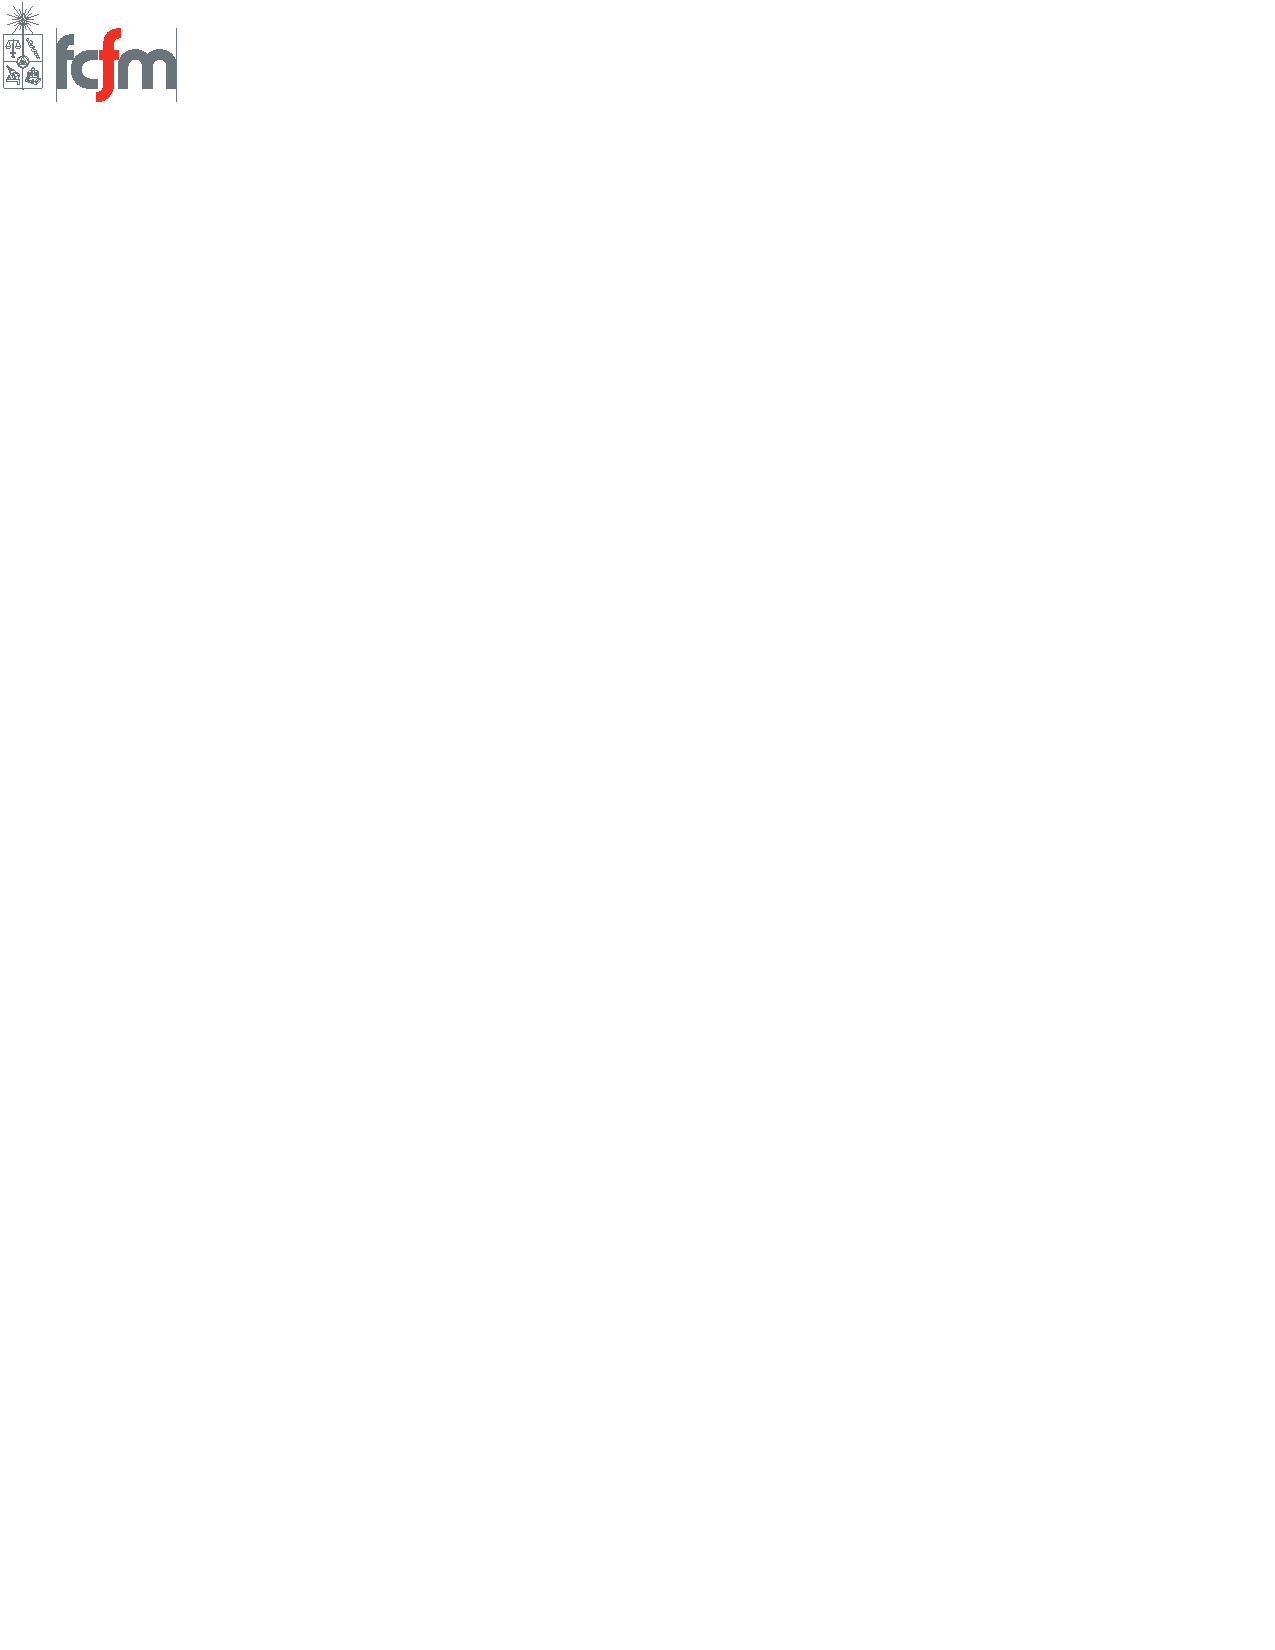
\includegraphics[scale=1.35]{departamentos/fcfm2}
	\end{wrapfigure}
	\hspace*{0.3cm}
	\noindent \textsc{\color{red} \hspace{-2.2cm} \departamentouniversidad} ~ \\
	\hspace*{0.3cm}
	\noindent \textsc{\color{dkgray} \hspace{-1.6cm} \nombrefacultad} ~ \\
	\hspace*{0.3cm}
	\noindent \textsc{\color{dkgray} \hspace{-1.6cm} \nombreuniversidad} ~ \\
	\hspace*{0.3cm}
	\noindent \textsc{\color{dkgray} \hspace{-1.6cm} \codigodelcurso \nombredelcurso} ~ \\
	\vfill
	\begin{center}
		\vspace*{0.5cm}
		{\color{dkgray} \Large \textbf{\MakeUppercase{\temaatratar}}} ~ \\
		\noindent \rule{\linewidth}{0.3mm} ~ \\
		\Huge \textup \bfseries \textsc{\textcolor{\portraittitlecolor}{\titulodelinforme}} ~ \\
		\noindent \rule{\linewidth}{0.3mm} ~ \\
	\end{center}
	\begin{minipage}{.5\textwidth}
		~
	\end{minipage}
	\vfill
	\begin{minipage}{1.0\textwidth}
		\begin{flushright}
			\noindent \tablaintegrantes
		\end{flushright}
	\end{minipage}
}{
\ifthenelse{\equal{\portraitstyle}{style7}}{
	\setpagemargincm{\pagemarginleft}{\pagemargintop}{\pagemarginright}{\pagemarginbottom}
	\thispagestyle{empty}
	\begin{center}
		\vspace*{-1.5cm}
		\includegraphics[scale=\imagendepartamentoescala]{\imagendepartamento}
		\hspace*{-0.15cm}
		\begin{tabular}{l}
			\vspace*{0.26cm}\mbox{} ~ \\
			\small \textsc{\MakeUppercase{\nombreuniversidad}} ~ \\
			\small \textsc{\MakeUppercase{\nombrefacultad}} ~ \\
			\small \textsc{\MakeUppercase{\departamentouniversidad}} ~ \\
			\vspace*{1.25cm}\mbox{}
		\end{tabular}
	\end{center}
	\vfill
	\begin{center}
		\noindent \rule{\textwidth}{0.4mm} \\ \vspace{0.3cm}
		{\huge \textcolor{\portraittitlecolor}{\titulodelinforme} \vspace{0.2cm} ~ \\}
		\noindent \rule{\textwidth}{0.4mm} ~ \\ \vspace{0.40cm}
		{\large \textcolor{\portraittitlecolor}{\temaatratar} ~ \\}
	\end{center}
	\vfill
	\noindent
	\begin{minipage}{1.0\textwidth}
		\begin{flushright}
			\scshape{\tablaintegrantes}
		\end{flushright}
	\end{minipage}
}{
\ifthenelse{\equal{\portraitstyle}{style8}}{
	\setpagemargincm{\pagemarginleft}{\pagemargintop}{\pagemarginright}{\pagemarginbottom}
	\thispagestyle{empty}
	\begin{center}
		\vspace*{-1.0cm}
		\begin{tabular}{c}
			\includegraphics[scale=\imagendepartamentoescala]{\imagendepartamento} \vspace{0.5cm} ~ \\
			\small \scshape{\MakeUppercase{\nombreuniversidad}} ~ \\
			\small \scshape{\MakeUppercase{\nombrefacultad}} ~ \\
			\small \scshape{\MakeUppercase{\departamentouniversidad}}
		\end{tabular}
	\end{center}
	\vfill
	\begin{center}
		\noindent \rule{\textwidth}{0.4mm} \\ \vspace{0.3cm}
		{\huge \textcolor{\portraittitlecolor}{\titulodelinforme} \vspace{0.2cm} ~ \\}
		\noindent \rule{\textwidth}{0.4mm} ~ \\ \vspace{0.40cm}
		{\large \textcolor{\portraittitlecolor}{\temaatratar} ~ \\}
	\end{center}
	\vfill
	\noindent
	\begin{minipage}{1.0\textwidth}
		\begin{flushright}
			\scshape{\tablaintegrantes}
		\end{flushright}
	\end{minipage}
}{
\ifthenelse{\equal{\portraitstyle}{style9}}{
	\setpagemargincm{\pagemarginleft}{\pagemargintop}{\pagemarginright}{\pagemarginbottom}
	\thispagestyle{empty}
	\noindent \includegraphics[scale=\imagendepartamentoescala]{\imagendepartamento}
	\vfill
	\begin{center}
		\noindent \rule{\textwidth}{0.4mm} \\ \vspace{0.3cm}
		{\huge \textcolor{\portraittitlecolor}{\titulodelinforme} \vspace{0.2cm} \\}
		\noindent \rule{\textwidth}{0.4mm} \\ \vspace{0.35cm}
		{\large \textcolor{\portraittitlecolor}{\temaatratar} \\}
	\end{center}
	\vfill
	\begin{center}
		\begin{tabular}{c}
			\small \scshape{\MakeUppercase{\nombreuniversidad}} ~ \\
			\small \scshape{\MakeUppercase{\nombrefacultad}} ~ \\
			\small \scshape{\MakeUppercase{\departamentouniversidad}}
		\end{tabular}
	\end{center}
	\vfill
	\begin{center}
		\indent \scshape{\tablaintegrantes}
	\end{center}
}{
\ifthenelse{\equal{\portraitstyle}{style10}}{
	\setpagemargincm{\pagemarginleft}{\pagemargintop}{\pagemarginright}{\pagemarginbottom}
	\thispagestyle{empty}
	~ \\
	\vfill
	\begin{center}
		\ifthenelse{\equal{\nombreuniversidad}{\xspace}}{
			\noindent {\large \textsc{\departamentouniversidad}}
		}{
			\noindent {\large \textsc{\nombreuniversidad, \departamentouniversidad}}
		}
		\vspace{1.0cm}
	\end{center}
	\vfill
	\begin{center}
		\noindent {\large \scshape{\nombredelcurso}} \vspace{0.5cm} ~ \\
		\noindent {\large \scshape{\codigodelcurso}} \vspace{0.5cm} ~ \\
		\noindent \rule{\textwidth}{0.4mm} \\ \vspace{0.3cm}
		{\huge \bfseries \textcolor{\portraittitlecolor}{\titulodelinforme} \vspace{0.2cm} \\}
		\noindent \rule{\textwidth}{0.4mm} \\ \vspace{2.5cm}
	\end{center}
	\vfill
	\begin{center}
		\indent \tablaintegrantes
	\end{center}
	\vfill
	~ \\
}{
\ifthenelse{\equal{\portraitstyle}{style11}}{
	\setpagemargincm{\pagemarginleft}{\pagemargintop}{\pagemarginright}{\pagemarginbottom}
	\thispagestyle{empty}
	\begin{center}
		\vspace*{-1.0cm}
		\scshape{\nombreuniversidad} ~ \\
		\scshape{\nombrefacultad} ~ \\
		\scshape{\departamentouniversidad}
	\end{center}
	\vfill
	\begin{center}
		{\setstretch{1.2} \fontsize{21pt}{22pt} \selectfont \textcolor{\portraittitlecolor}{\scshape{\titulodelinforme}} \vspace{0.5cm}} ~ \\
		{\fontsize{13pt}{10pt} \selectfont \textcolor{\portraittitlecolor}{\scshape{\temaatratar}}}
	\end{center}
	\vfill
	\begin{center}
		\indent \tablaintegrantes
	\end{center}
}{
\ifthenelse{\equal{\portraitstyle}{style12}}{
	\setpagemargincm{\pagemarginleft}{\pagemargintop}{\pagemarginright}{\pagemarginbottom}
	\thispagestyle{empty}
	\begin{center}
		\vspace*{-1.0cm}
		\includegraphics[scale=\imagendepartamentoescala]{\imagendepartamento}
	\end{center}
	\vfill
	\begin{center}
		{\bf \Huge \scshape{\textcolor{\portraittitlecolor}{\titulodelinforme}} \vspace{0.3cm}} \\
		{\bf \Large \textcolor{\portraittitlecolor}{\temaatratar}}
	\end{center}
	\vfill
	\begin{flushright}
		\noindent \tablaintegrantes
	\end{flushright}
	\vspace{0.5cm}
	\noindent \rule{\textwidth}{0.4mm}
	\begin{center}
		\ifthenelse{\equal{\nombreuniversidad}{\xspace}}{
			\scshape{\nombrefacultad} \\
		}{
			\scshape{\nombreuniversidad, \nombrefacultad} \\
		}
		\scshape{\departamentouniversidad}
	\end{center}
}{
\ifthenelse{\equal{\portraitstyle}{style13}}{
	\setpagemargincm{\pagemarginleft}{\pagemargintop}{\pagemarginright}{\pagemarginbottom}
	\thispagestyle{empty}
	\noindent
	\vspace*{-1.5cm}
	\begin{flushleft}
		\begin{minipage}{0.65\textwidth}
			\ifthenelse{\equal{\nombreuniversidad}{\xspace}}{
				{\fontsize{3.5mm}{0.5mm} \selectfont \noindent \textsf{\nombrefacultad}} ~ \\
			}{
				{\fontsize{3.5mm}{0.5mm} \selectfont \noindent \textsf{\nombreuniversidad, \nombrefacultad}} ~ \\
			}
			\noindent {\fontsize{3.0mm}{0.5mm} \selectfont \textsf{\departamentouniversidad} \vspace{-0.2cm}} ~ \\
			\noindent \textcolor{gray}{\rule{\textwidth}{0.3mm}}
		\end{minipage}
	\end{flushleft}
	\vspace*{-2.15cm}
	\begin{flushright}
		\begin{minipage}{0.3\textwidth}
			\noindent \includegraphics[width=1.0\textwidth]{\imagendepartamento}
		\end{minipage}
	\end{flushright}
	\vfill
	\begin{center}
		\begin{minipage}{0.9\textwidth}
			\begin{framed}
				\LARGE
				\vspace{1cm}
				\centering \textcolor{\portraittitlecolor}{\textbf{\titulodelinforme}}
				\vspace{1cm}
			\end{framed}
		\end{minipage}
	\end{center}
	\vfill
	\begin{flushright}
		\noindent \textsf{\tablaintegrantes}
	\end{flushright}
}{
\ifthenelse{\equal{\portraitstyle}{style14}}{
	\setpagemargincm{\pagemarginleft}{\pagemargintop}{\pagemarginright}{\pagemarginbottom}
	\thispagestyle{empty}
	\noindent
	\begin{flushleft}
		\vspace*{-1.0cm}
		\noindent \includegraphics[scale=\imagendepartamentoescala]{\imagendepartamento} \\
	\end{flushleft}
	\vfill
	{\bf \huge \noindent \textcolor{\portraittitlecolor}{\textsf{\MakeUppercase{\titulodelinforme}} \vspace*{0.05cm}}} \\
	{\bf \large \noindent \textcolor{\portraittitlecolor}{\textsf{\MakeUppercase{\temaatratar}}}} \\
	\vfill
	\begin{flushright}
		\noindent \textsf{\tablaintegrantes}
	\end{flushright}
}{
\ifthenelse{\equal{\portraitstyle}{style15}}{
	\setpagemargincm{\pagemarginleft}{\pagemargintop}{\pagemarginright}{\pagemarginbottom}
	\thispagestyle{empty}
	\checkextravarexist{\headerimageA}{Defina la imagen extra de la portada en el archivo lib/page/portrait-config.tex (VERSION NORMAL) o bien en el bloque PORTADA (VERSION COMPACTA)}
	\checkextravarexist{\headerimagescaleA}{Defina la escala de la imagen extra de la portada en el archivo lib/page/portrait-config.tex (VERSION NORMAL) o bien en el bloque PORTADA (VERSION COMPACTA)}
	\vspace*{-1.5cm}
	\noindent \begin{minipage}{0.8\textwidth}
		\noindent \begin{minipage}{0.22\textwidth}
			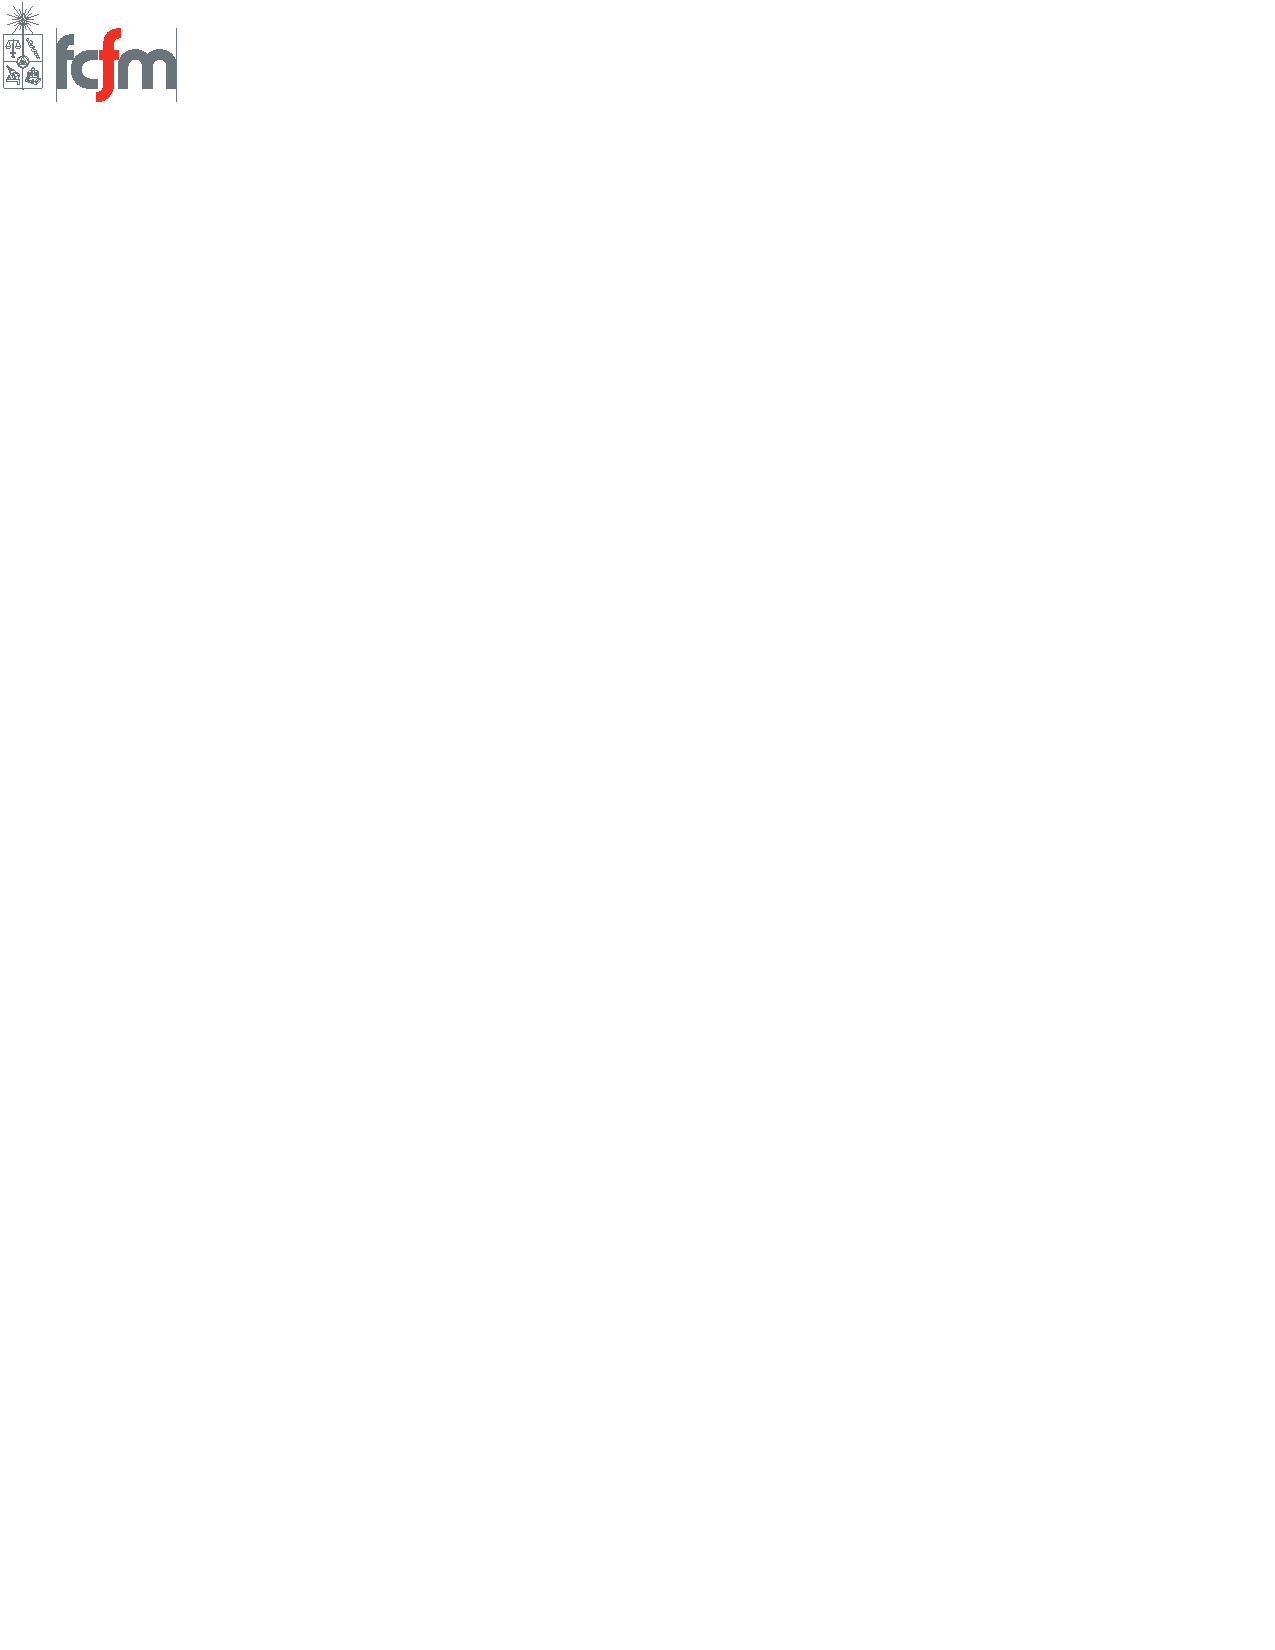
\includegraphics[scale=1.0]{departamentos/fcfm2} \\
		\end{minipage}
		\begin{minipage}{0.6\textwidth}
			\begin{flushleft}
				\textsc{
				\begin{tabular}{l}
					{\small \nombreuniversidad} ~ \\
					{\small \nombrefacultad} ~ \\
					{\small \departamentouniversidad}
				\end{tabular}
				}
			\end{flushleft}
		\end{minipage}
	\end{minipage}
	\noindent \begin{minipage}{0.2\textwidth}
		\begin{flushright}
			\ifthenelse{\isundefined{\headerimageA}}{}{
				\ifthenelse{\isundefined{\headerimagescaleA}}{}{
					\noindent \includegraphics[scale=\headerimagescaleA]{\headerimageA} \\
				}
			}
		\end{flushright}
	\end{minipage}
	\vfill
	\begin{center}
		{\fontsize{25pt}{15pt} \selectfont \textcolor{\portraittitlecolor}{\textbf{\titulodelinforme}} \vspace{0.7cm}} \\
		{\Large \textcolor{\portraittitlecolor}{\temaatratar}}
	\end{center}
	\vfill
	\begin{center}
		\noindent \tablaintegrantes
	\end{center}
}{
\ifthenelse{\equal{\portraitstyle}{style16}}{
	\setpagemargincm{\pagemarginleft}{\pagemargintop}{\pagemarginright}{\pagemarginbottom}
	\checkextravarexist{\portraitbackgroundimageB}{[portrait-style16] Defina el fondo de la portada en el archivo lib/page/portrait-config.tex (VERSION NORMAL) o bien en el bloque PORTADA (VERSION COMPACTA)}
	\checkextravarexist{\portraitbackgroundcolorB}{[portrait-style16] Defina el color del bloque del titulo de la portada en el archivo lib/page/portrait-config.tex (VERSION NORMAL) o bien en el bloque PORTADA (VERSION COMPACTA)}
	\begingroup
		\thispagestyle{empty}
		\begin{tikzpicture}[remember picture,overlay]
			\node[inner sep=0pt] (background) at (current page.center) {\includegraphics[width=\paperwidth]{\portraitbackgroundimageB}};
			\draw (current page.center) node [fill=\portraitbackgroundcolorB!30!white,fill opacity=0.6,text opacity=1,inner sep=1cm]{\Huge\centering\bfseries\sffamily\parbox[c][][t]{\paperwidth}{
					\centering \textcolor{\portraittitlecolor}{\titulodelinforme} \\ [10pt]
					{\Large \temaatratar} \\ [25pt]
					{\huge \autordeldocumento}}};
		\end{tikzpicture}
		\vfill
	\endgroup
}{
\ifthenelse{\equal{\portraitstyle}{style17}}{
	\setpagemargincm{\pagemarginleft}{\firstpagemargintop}{\pagemarginright}{\pagemarginbottom}
	\pagestyle{fancy}
	\checkextravarexist{\portraitimageC}{[portrait-style17] Defina la imagen de la portada en el archivo lib/page/portrait-config.tex (VERSION NORMAL) o bien en el bloque PORTADA (VERSION COMPACTA)}
	\checkextravarexist{\portraitimageboxedC}{[portrait-style17] Defina si la imagen de la portada se encierra en un recuadro en el archivo lib/page/portrait-config.tex (VERSION NORMAL) o bien en el bloque PORTADA (VERSION COMPACTA)}
	\checkextravarexist{\portraitimageboxedwidthC}{[portrait-style17] Defina el grosor del recuadro de la imagen de la portada en el archivo lib/page/portrait-config.tex (VERSION NORMAL) o bien en el bloque PORTADA (VERSION COMPACTA)}
	\checkextravarexist{\portraitimagewidthC}{[portrait-style17] Defina los parametros de la imagen de la portada en el archivo lib/page/portrait-config.tex (VERSION NORMAL) o bien en el bloque PORTADA (VERSION COMPACTA)}
	\fancyhf{}
	\fancyhead[L]{
		\nombreuniversidad ~ \\
		\nombrefacultad ~ \\
		\departamentouniversidad ~ \\
		\vspace{-0.43cm}
	}
	\fancyhead[R]{
		\includegraphics[scale=\imagendepartamentoescala]{\imagendepartamento}
		\hspace{-0.255cm}
	}
	~ \\
	\vfill
	\begin{center}
		\textcolor{\portraittitlecolor}{
			{\noindent \Huge{\titulodelinforme} \vspace{0.5cm}} ~ \\
			{\noindent \large{\temaatratar}}
		}
	\end{center}
	~ \\
	\ifthenelse{\equal{\portraitimageboxedC}{true}}{
		\insertimageboxed{\portraitimageC}{width=\portraitimagewidthC}{\portraitimageboxedwidthC}{}
	}{
		\insertimage{\portraitimageC}{width=\portraitimagewidthC}{}
	}
	~ \\
	\vfill
	\noindent
	\begin{minipage}{1.0\textwidth}
		\begin{flushright}
			\tablaintegrantes
		\end{flushright}
	\end{minipage}
}{
\ifthenelse{\equal{\portraitstyle}{style18}}{
	\setpagemargincm{\pagemarginleft}{\firstpagemargintop}{\pagemarginright}{\pagemarginbottom}
	\pagestyle{fancy}
	\checkextravarexist{\portraitimageD}{[portrait-style18] Defina la imagen de la portada en el archivo lib/page/portrait-config.tex (VERSION NORMAL) o bien en el bloque PORTADA (VERSION COMPACTA)}
	\checkextravarexist{\portraitimageboxedD}{[portrait-style18] Defina si la imagen de la portada se encierra en un recuadro en el archivo lib/page/portrait-config.tex (VERSION NORMAL) o bien en el bloque PORTADA (VERSION COMPACTA)}
	\checkextravarexist{\portraitimageboxedwidthD}{[portrait-style18] Defina el grosor del recuadro de la imagen de la portada en el archivo lib/page/portrait-config.tex (VERSION NORMAL) o bien en el bloque PORTADA (VERSION COMPACTA)}
	\checkextravarexist{\portraitimagewidthD}{[portrait-style18] Defina los parametros de la imagen de la portada en el archivo lib/page/portrait-config.tex (VERSION NORMAL) o bien en el bloque PORTADA (VERSION COMPACTA)}
	\fancyhf{}
	\fancyhead[L]{
		\nombreuniversidad ~ \\
		\nombrefacultad ~ \\
		\departamentouniversidad ~ \\
		\vspace{-0.43cm}
	}
	\fancyhead[R]{
		\includegraphics[scale=\imagendepartamentoescala]{\imagendepartamento}
		\hspace{-0.255cm}
	}
	~ \\
	\ifthenelse{\equal{\portraitimageboxedD}{true}}{
		\insertimageboxed{\portraitimageD}{width=\portraitimagewidthD}{\portraitimageboxedwidthD}{}
	}{
		\insertimage{\portraitimageD}{width=\portraitimagewidthD}{}
	}
	\vfill
	\begin{center}
		\textcolor{\portraittitlecolor}{
			{\noindent \Huge{\titulodelinforme} \vspace{0.5cm}} ~ \\
			{\noindent \large{\temaatratar}}
		}
	\end{center}
	\vfill
	\noindent
	\begin{minipage}{1.0\textwidth}
		\begin{flushright}
			\tablaintegrantes
		\end{flushright}
	\end{minipage}
}{
\ifthenelse{\equal{\portraitstyle}{\bgtemplatetestcode}}{
	\setpagemargincm{\pagemarginleft}{\pagemargintop}{\pagemarginright}{\pagemarginbottom}
	\pagestyle{empty}
	\pagecolor{lbrown}
	\begin{center}
		\vspace*{-1.0cm}
		\scshape{\nombreuniversidad} ~ \\
		\scshape{\nombrefacultad} ~ \\
		\scshape{\departamentouniversidad}
	\end{center}
	~ \\
	\begin{center}
		\bgtemplatetestimg
	\end{center}
	\begin{center}
		\vspace*{-6cm}
		{\setstretch{1.2} \fontsize{25pt}{22pt} \selectfont \textcolor{\portraittitlecolor}{\scshape{\titulodelinforme}} \vspace{0.5cm}} \\
		{\fontsize{15pt}{10pt} \selectfont \textcolor{\portraittitlecolor}{\scshape{\temaatratar}}}
	\end{center}
	\vfill
	\begin{flushright}
		\noindent \tablaintegrantes
	\end{flushright}
	\newpage
	\pagecolor{white}
}{
	\throwbadconfigondoc{Estilo de portada incorrecto}{\portraitstyle}{style1 .. style18}}}}}}}}}}}}}}}}}}}
}
\ifthenelse{\equal{\addemptypagetwosides}{true}}{
	\newpage
	\null
	\thispagestyle{empty}
	\renewcommand{\thepage}{}
	\newpage}{
}
 % Se puede borrar

% CONFIGURACIÓN DE PÁGINA Y ENCABEZADOS
% Template:     Informe/Reporte LaTeX
% Documento:    Configuración de página
% Versión:      6.2.2 (30/01/2019)
% Codificación: UTF-8
%
% Autor: Pablo Pizarro R. @ppizarror
%        Facultad de Ciencias Físicas y Matemáticas
%        Universidad de Chile
%        pablo.pizarro@ing.uchile.cl, ppizarror.com
%
% Manual template: [https://latex.ppizarror.com/Template-Informe/]
% Licencia MIT:    [https://opensource.org/licenses/MIT/]

\newpage
\ifthenelse{\equal{\predocuseromannumber}{true}}{
	\ifthenelse{\equal{\romanpageuppercase}{true}}{
		\pagenumbering{Roman}
	}{
		\pagenumbering{roman}
	}}{
	\pagenumbering{arabic}
}
\setcounter{page}{1}
\setcounter{footnote}{1}
\setpagemargincm{\pagemarginleft}{\pagemargintop}{\pagemarginright}{\pagemarginbottom}
\def\arraystretch {\tablepaddingv}
\setlength{\tabcolsep}{\tablepaddingh em}
\ifthenelse{\equal{\pointdecimal}{true}}{
	\decimalpoint}{
}
\renewcommand{\appendixname}{\nomltappendixsection}
\renewcommand{\appendixpagename}{\nameappendixsection}
\renewcommand{\appendixtocname}{\nameappendixsection}
\renewcommand{\contentsname}{\nomltcont}
\renewcommand{\figurename}{\nomltwfigure}
\renewcommand{\listfigurename}{\nomltfigure}
\renewcommand{\listtablename}{\nomlttable}
\renewcommand{\lstlistingname}{\nomltwsrc}
\renewcommand{\lstlistlistingname}{\nomltsrc}
\renewcommand{\refname}{\namereferences}
\renewcommand{\tablename}{\nomltwtable}
\sectionfont{\color{\titlecolor} \fontsizetitle \styletitle \selectfont}
\subsectionfont{\color{\subtitlecolor} \fontsizesubtitle \stylesubtitle \selectfont}
\subsubsectionfont{\color{\subsubtitlecolor} \fontsizesubsubtitle \stylesubsubtitle \selectfont}
\titleformat{\subsubsubsection}{\color{\ssstitlecolor} \normalfont \fontsizessstitle \stylessstitle}{\thesubsubsubsection}{1em}{}
\titlespacing*{\subsubsubsection}{0pt}{3.25ex plus 1ex minus .2ex}{1.5ex plus .2ex}
\ifthenelse{\equal{\hfstyle}{style1}}{
	\pagestyle{fancy} \fancyhf{}
	\ifthenelse{\equal{\disablehfrightmark}{false}}{
		\fancyhead[L]{\nouppercase{\rightmark}}
	}{}
	\fancyhead[R]{\small \rm \thepage}
	\fancyfoot[L]{\small \rm \textit{\titulodelinforme}}
	\fancyfoot[R]{\small \rm \textit{\codigodelcurso \nombredelcurso}}
	\renewcommand{\headrulewidth}{0.5pt}
	\renewcommand{\footrulewidth}{0.5pt}
	\renewcommand{\sectionmark}[1]{\markboth{#1}{}}
}{
\ifthenelse{\equal{\hfstyle}{style2}}{
	\pagestyle{fancy} \fancyhf{}
	\ifthenelse{\equal{\disablehfrightmark}{false}}{
		\fancyhead[L]{\nouppercase{\rightmark}}
	}{}
	\fancyhead[R]{\small \rm \thepage}
	\fancyfoot[L]{\small \rm \textit{\titulodelinforme}}
	\fancyfoot[R]{\small \rm \textit{\codigodelcurso \nombredelcurso}}
	\renewcommand{\headrulewidth}{0.5pt}
	\renewcommand{\footrulewidth}{0pt}
	\renewcommand{\sectionmark}[1]{\markboth{#1}{}}
}{
\ifthenelse{\equal{\hfstyle}{style3}}{
	\pagestyle{fancy} \fancyhf{}
	\fancyhead[L]{
		\small \rm \textit{\codigodelcurso \nombredelcurso}
		\vspace{0.04cm}
	}
	\fancyhead[R]{
		\includegraphics[width=1.2cm]{\imagendepartamento}
		\vspace{-0.10cm}
	}
	\fancyfoot[C]{\thepage}
	\renewcommand{\headrulewidth}{0.5pt}
	\renewcommand{\footrulewidth}{0pt}
}{
\ifthenelse{\equal{\hfstyle}{style4}}{
	\pagestyle{fancy} \fancyhf{}
	\ifthenelse{\equal{\disablehfrightmark}{false}}{
		\fancyhead[L]{\nouppercase{\rightmark}}
	}{}
	\fancyhead[R]{}
	\fancyfoot[C]{\small \rm \thepage}
	\renewcommand{\headrulewidth}{0.5pt}
	\renewcommand{\footrulewidth}{0pt}
	\renewcommand{\sectionmark}[1]{\markboth{#1}{}}
}{
\ifthenelse{\equal{\hfstyle}{style5}}{
	\pagestyle{fancy} \fancyhf{}
	\fancyhead[L]{\codigodelcurso \nombredelcurso}
	\ifthenelse{\equal{\disablehfrightmark}{false}}{
		\fancyhead[R]{\nouppercase{\rightmark}}
	}{}
	\fancyfoot[L]{\departamentouniversidad, \nombreuniversidad}
	\fancyfoot[R]{\small \rm \thepage}
	\renewcommand{\headrulewidth}{0pt}
	\renewcommand{\footrulewidth}{0pt}
	\renewcommand{\sectionmark}[1]{\markboth{#1}{}}
}{
\ifthenelse{\equal{\hfstyle}{style6}}{
	\pagestyle{fancy} \fancyhf{}
	\fancyfoot[L]{\departamentouniversidad}
	\fancyfoot[C]{\thepage}
	\fancyfoot[R]{\nombreuniversidad}
	\renewcommand{\headrulewidth}{0pt}
	\renewcommand{\footrulewidth}{0pt}
	\setlength{\headheight}{49pt}
}{
\ifthenelse{\equal{\hfstyle}{style7}}{
	\pagestyle{fancy} \fancyhf{}
	\fancyfoot[C]{\thepage}
	\renewcommand{\headrulewidth}{0pt}
	\renewcommand{\footrulewidth}{0pt}
	\setlength{\headheight}{49pt}
}{
\ifthenelse{\equal{\hfstyle}{style8}}{
	\pagestyle{fancy} \fancyhf{}
	\fancyfoot[R]{\thepage}
	\renewcommand{\headrulewidth}{0pt}
	\renewcommand{\footrulewidth}{0pt}
	\setlength{\headheight}{49pt}
}{
\ifthenelse{\equal{\hfstyle}{style9}}{
	\pagestyle{fancy} \fancyhf{}
	\ifthenelse{\equal{\disablehfrightmark}{false}}{
		\fancyhead[L]{\nouppercase{\rightmark}}
	}{}
	\fancyhead[R]{}
	\fancyfoot[L]{\small \rm \textit{\titulodelinforme}}
	\fancyfoot[R]{\small \rm \thepage}
	\renewcommand{\headrulewidth}{0.5pt}
	\renewcommand{\footrulewidth}{0.5pt}
	\renewcommand{\sectionmark}[1]{\markboth{#1}{}}
}{
\ifthenelse{\equal{\hfstyle}{style10}}{
	\pagestyle{fancy} \fancyhf{}
	\ifthenelse{\equal{\disablehfrightmark}{false}}{
		\fancyhead[L]{\nouppercase{\rightmark}}
	}{}
	\fancyhead[R]{\small \rm \textit{\titulodelinforme}}
	\fancyfoot[L]{}
	\fancyfoot[R]{\small \rm \thepage}
	\renewcommand{\headrulewidth}{0.5pt}
	\renewcommand{\footrulewidth}{0.5pt}
	\renewcommand{\sectionmark}[1]{\markboth{#1}{}}
}{
\ifthenelse{\equal{\hfstyle}{style11}}{
	\pagestyle{fancy} \fancyhf{}
	\ifthenelse{\equal{\disablehfrightmark}{false}}{
		\fancyhead[L]{\nouppercase{\rightmark}}
	}{}
	\fancyhead[R]{\small \rm \thepage \nomnpageof \pageref{LastPage}}
	\fancyfoot[L]{\small \rm \textit{\titulodelinforme}}
	\fancyfoot[R]{\small \rm \textit{\codigodelcurso \nombredelcurso}}
	\renewcommand{\headrulewidth}{0.5pt}
	\renewcommand{\footrulewidth}{0.5pt}
	\renewcommand{\sectionmark}[1]{\markboth{#1}{}}
}{
\ifthenelse{\equal{\hfstyle}{style12}}{
	\pagestyle{fancy} \fancyhf{}
	\fancyfoot[L]{\departamentouniversidad}
	\fancyfoot[C]{\thepage \nomnpageof \pageref{LastPage}}
	\fancyfoot[R]{\nombreuniversidad}
	\renewcommand{\headrulewidth}{0pt}
	\renewcommand{\footrulewidth}{0pt}
	\setlength{\headheight}{49pt}
}{
\ifthenelse{\equal{\hfstyle}{style13}}{
	\pagestyle{fancy} \fancyhf{}
	\fancyhead[L]{
		\small \rm \textit{\codigodelcurso \nombredelcurso}
		\vspace{0.04cm}
	}
	\fancyhead[R]{
		\includegraphics[width=1.2cm]{\imagendepartamento}
		\vspace{-0.10cm}
	}
	\fancyfoot[C]{\thepage \nomnpageof \pageref{LastPage}}
	\renewcommand{\headrulewidth}{0.5pt}
	\renewcommand{\footrulewidth}{0pt}
}{
\ifthenelse{\equal{\hfstyle}{style14}}{
	\pagestyle{fancy} \fancyhf{}
	\ifthenelse{\equal{\disablehfrightmark}{false}}{
		\fancyhead[L]{\nouppercase{\rightmark}}
	}{}
	\fancyhead[R]{}
	\fancyfoot[C]{\small \rm \thepage \nomnpageof \pageref{LastPage}}
	\renewcommand{\headrulewidth}{0.5pt}
	\renewcommand{\footrulewidth}{0pt}
	\renewcommand{\sectionmark}[1]{\markboth{#1}{}}
}{
	\throwbadconfigondoc{Estilo de header-footer incorrecto}{\hfstyle}{style1 .. style14}}}}}}}}}}}}}}
}
\ifthenelse{\equal{\showlinenumbers}{true}}{
	\linenumbers}{
}


% Template:     Informe/Reporte LaTeX
% Documento:    Índice
% Versión:      6.2.2 (30/01/2019)
% Codificación: UTF-8
%
% Autor: Pablo Pizarro R. @ppizarror
%        Facultad de Ciencias Físicas y Matemáticas
%        Universidad de Chile
%        pablo.pizarro@ing.uchile.cl, ppizarror.com
%
% Manual template: [https://latex.ppizarror.com/Template-Informe/]
% Licencia MIT:    [https://opensource.org/licenses/MIT/]

\ifthenelse{\equal{\showindex}{true}}{
	\newpage
	\begingroup
	\sectionfont{\color{\indextitlecolor} \fontsizetitlei \styletitlei \selectfont}
	\ifthenelse{\equal{\addemptypagetwosides}{true}}{
		\checkoddpage
		\ifoddpage
		\else
			\newpage
			\null
			\thispagestyle{empty}
			\newpage
			\addtocounter{page}{-1}
		\fi}{
	}
	\ifthenelse{\equal{\addindextobookmarks}{true}}{
		\belowpdfbookmark{\nomltcont}{contents}}{
	}
	\tocloftpagestyle{fancy}
	\ifthenelse{\equal{\showdotaftersnum}{true}}{
		\def\cftsecaftersnum {.}
		\def\cftsubsecaftersnum {.}
		\def\cftsubsubsecaftersnum {.}
		\def\cftsubsubsubsecaftersnum {.}
		\def\cftsecnumwidth {1.9em}
\def\cftsubsecnumwidth {2.57em}
\renewcommand\cftsubsubsecnumwidth{3.35em}
		\setlength{\cftsubsecindent}{1.91em}
\setlength{\cftsubsubsecindent}{4.48em}
		}{
	}
	\renewcommand{\cftdot}{\charnumpageindex}
	\def\cftfigaftersnum {\charafterobjectindex\enspace}
	\def\cftsubfigaftersnum {\charafterobjectindex\enspace}
	\def\cfttabaftersnum {\charafterobjectindex\enspace}
	\def\cftlstlistingaftersnum {\charafterobjectindex\enspace}
	\ifthenelse{\equal{\showlinenumbers}{true}}{
		\nolinenumbers}{
	}
	\ifthenelse{\equal{\objectindexindent}{true}}{
		\def\cftlstlistingindent {1.495em}
	}{
		\setlength{\cfttabindent}{0in}
		\setlength{\cftfigindent}{0in}
		\setlength{\cftsubfigindent}{0in}
		\setlength{\cftfigindent}{0in}
		\def\cftlstlistingindent {0.01em}
	}
	\ifthenelse{\equal{\equalmarginnumobject}{true}}{
		\ifthenelse{\equal{\showsectioncaption}{none}}{
			\def\cftdefautnumwidth {2.3em}
		}{
		\ifthenelse{\equal{\showsectioncaption}{sec}}{
			\def\cftdefautnumwidth {3.0em}
		}{
		\ifthenelse{\equal{\showsectioncaption}{ssec}}{
			\def\cftdefautnumwidth {3.7em}
		}{
		\ifthenelse{\equal{\showsectioncaption}{sssec}}{
			\def\cftdefautnumwidth {4.4em}
		}{
		\ifthenelse{\equal{\showsectioncaption}{ssssec}}{
			\def\cftdefautnumwidth {5.1em}
		}{
			\throwbadconfig{Valor configuracion incorrecto}{\showsectioncaption}{none,sec,ssec,sssec,ssssec}}}}}
		}
		\def\cftfignumwidth {\cftdefautnumwidth}
		\def\cftsubfignumwidth {\cftdefautnumwidth}
		\def\cfttabnumwidth {\cftdefautnumwidth}
		\def\cftlstlistingnumwidth {\cftdefautnumwidth}}{
	}
	\newcommand{\coregeneratefigureindex}{
		\iftotalfigures
			\ifthenelse{\equal{\indexnewpagef}{true}}{\newpage}{}
			\listoffigures
		\fi
	}
	\newcommand{\coregeneratetableindex}{
		\iftotaltables
			\ifthenelse{\equal{\indexnewpaget}{true}}{\newpage}{}
			\listoftables
		\fi
	}
	\newcommand{\coregeneratecodeindex}{
		\iftotallstlistings
			\ifthenelse{\equal{\indexnewpagec}{true}}{\newpage}{}
			\lstlistoflistings
		\fi
	}
	\ifthenelse{\equal{\showindexofcontents}{true}}{
		\tableofcontents
	}{}
	\ifthenelse{\equal{\indexstyle}{ftc}}{
		\coregeneratefigureindex
		\coregeneratetableindex
		\coregeneratecodeindex
	}{
	\ifthenelse{\equal{\indexstyle}{f}}{
		\coregeneratefigureindex
	}{
	\ifthenelse{\equal{\indexstyle}{ft}}{
		\coregeneratefigureindex
		\coregeneratetableindex
	}{
	\ifthenelse{\equal{\indexstyle}{fc}}{
		\coregeneratefigureindex
		\coregeneratecodeindex
	}{
	\ifthenelse{\equal{\indexstyle}{fct}}{
		\coregeneratefigureindex
		\coregeneratecodeindex
		\coregeneratetableindex
	}{
	\ifthenelse{\equal{\indexstyle}{t}}{
		\coregeneratetableindex
	}{
	\ifthenelse{\equal{\indexstyle}{tf}}{
		\coregeneratetableindex
		\coregeneratefigureindex
	}{
	\ifthenelse{\equal{\indexstyle}{tfc}}{
		\coregeneratetableindex
		\coregeneratefigureindex
		\coregeneratecodeindex
	}{
	\ifthenelse{\equal{\indexstyle}{tc}}{
		\coregeneratetableindex
		\coregeneratecodeindex
	}{
	\ifthenelse{\equal{\indexstyle}{tcf}}{
		\coregeneratetableindex
		\coregeneratecodeindex
		\coregeneratefigureindex
	}{
	\ifthenelse{\equal{\indexstyle}{c}}{
		\coregeneratecodeindex
	}{
	\ifthenelse{\equal{\indexstyle}{ct}}{
		\coregeneratecodeindex
		\coregeneratetableindex
	}{
	\ifthenelse{\equal{\indexstyle}{ctf}}{
		\coregeneratecodeindex
		\coregeneratetableindex
		\coregeneratefigureindex
	}{
	\ifthenelse{\equal{\indexstyle}{cf}}{
		\coregeneratecodeindex
		\coregeneratefigureindex
	}{
	\ifthenelse{\equal{\indexstyle}{cft}}{
		\coregeneratecodeindex
		\coregeneratefigureindex
		\coregeneratetableindex
	}{
	\ifthenelse{\equal{\indexstyle}{}}{
	}{
		\throwbadconfig{Estilo desconocido del indice}{\indexstyle}{,f,ft,ftc,fc,fct,t,tf,tfc,tc,tcf,c,ct,ctf,cf,cft}}}}}}}}}}}}}}}}
	}
	\endgroup
	\newpage
	\ifthenelse{\equal{\addemptypagetwosides}{true}}{
		\vfill
		\checkoddpage
		\ifoddpage
			\newpage
			\null
			\thispagestyle{empty}
			\newpage
			\addtocounter{page}{-1}
		\else
		\fi}{
	}
}{}
 % Se puede borrar

% CONFIGURACIONES FINALES
% Template:     Informe/Reporte LaTeX
% Documento:    Configuraciones finales
% Versión:      6.2.2 (30/01/2019)
% Codificación: UTF-8
%
% Autor: Pablo Pizarro R. @ppizarror
%        Facultad de Ciencias Físicas y Matemáticas
%        Universidad de Chile
%        pablo.pizarro@ing.uchile.cl, ppizarror.com
%
% Manual template: [https://latex.ppizarror.com/Template-Informe/]
% Licencia MIT:    [https://opensource.org/licenses/MIT/]

\markboth{}{}
\newpage
\ifthenelse{\equal{\disablehfrightmark}{false}}{
	\ifthenelse{\equal{\hfstyle}{style1}}{
		\fancyhead[L]{\nouppercase{\leftmark}}}{
	}
	\ifthenelse{\equal{\hfstyle}{style2}}{
		\fancyhead[L]{\nouppercase{\leftmark}}}{
	}
	\ifthenelse{\equal{\hfstyle}{style4}}{
		\fancyhead[L]{\nouppercase{\leftmark}}}{
	}
	\ifthenelse{\equal{\hfstyle}{style5}}{
		\fancyhead[R]{\nouppercase{\leftmark}}}{
	}
	\ifthenelse{\equal{\hfstyle}{style9}}{
		\fancyhead[L]{\nouppercase{\leftmark}}}{
	}
	\ifthenelse{\equal{\hfstyle}{style10}}{
		\fancyhead[L]{\nouppercase{\leftmark}}}{
	}
\ifthenelse{\equal{\hfstyle}{style11}}{
		\fancyhead[L]{\nouppercase{\leftmark}}}{
	}
\ifthenelse{\equal{\hfstyle}{style14}}{
		\fancyhead[L]{\nouppercase{\leftmark}}}{
	}}{
}
\sectionfont{\color{\titlecolor} \fontsizetitle \styletitle \selectfont}
\subsectionfont{\color{\subtitlecolor} \fontsizesubtitle \stylesubtitle \selectfont}
\subsubsectionfont{\color{\subsubtitlecolor} \fontsizesubsubtitle \stylesubsubtitle \selectfont}
\titleformat{\subsubsubsection}{\color{\ssstitlecolor} \normalfont \fontsizessstitle \stylessstitle}{\thesubsubsubsection}{1em}{}
\titlespacing*{\subsubsubsection}{0pt}{3.25ex plus 1ex minus .2ex}{1.5ex plus .2ex}
\ifthenelse{\equal{\showsectioncaption}{none}}{
}{
\ifthenelse{\equal{\showsectioncaption}{sec}}{
	\counterwithin{equation}{section}
	\counterwithin{figure}{section}
	\counterwithin{lstlisting}{section}
	\counterwithin{table}{section}
}{
\ifthenelse{\equal{\showsectioncaption}{ssec}}{
	\counterwithin{equation}{subsection}
	\counterwithin{figure}{subsection}
	\counterwithin{lstlisting}{subsection}
	\counterwithin{table}{subsection}
}{
\ifthenelse{\equal{\showsectioncaption}{sssec}}{
	\counterwithin{equation}{subsubsection}
	\counterwithin{figure}{subsubsection}
	\counterwithin{lstlisting}{subsubsection}
	\counterwithin{table}{subsubsection}
}{
\ifthenelse{\equal{\showsectioncaption}{ssssec}}{
	\counterwithin{equation}{subsubsubsection}
	\counterwithin{figure}{subsubsubsection}
	\counterwithin{lstlisting}{subsubsubsection}
	\counterwithin{table}{subsubsubsection}
}{
	\throwbadconfig{Valor configuracion incorrecto}{\showsectioncaption}{none,sec,ssec,sssec,ssssec}
}}}}}
\ifthenelse{\equal{\captionnumfigure}{arabic}}{
	\renewcommand{\thefigure}{\arabic{figure}}
}{
\ifthenelse{\equal{\captionnumfigure}{alph}}{
	\renewcommand{\thefigure}{\alph{figure}}
}{
\ifthenelse{\equal{\captionnumfigure}{Alph}}{
	\renewcommand{\thefigure}{\Alph{figure}}
}{
\ifthenelse{\equal{\captionnumfigure}{roman}}{
	\renewcommand{\thefigure}{\roman{figure}}
}{
\ifthenelse{\equal{\captionnumfigure}{Roman}}{
	\renewcommand{\thefigure}{\Roman{figure}}
}{
	\throwbadconfig{Tipo numero figura desconocido}{\captionnumfigure}{arabic,alph,Alph,roman,Roman}}}}}
}
\ifthenelse{\equal{\captionnumsubfigure}{arabic}}{
	\renewcommand{\thesubfigure}{\arabic{subfigure}}
}{
\ifthenelse{\equal{\captionnumsubfigure}{alph}}{
	\renewcommand{\thesubfigure}{\alph{subfigure}}
}{
\ifthenelse{\equal{\captionnumsubfigure}{Alph}}{
	\renewcommand{\thesubfigure}{\Alph{subfigure}}
}{
\ifthenelse{\equal{\captionnumsubfigure}{roman}}{
	\renewcommand{\thesubfigure}{\roman{subfigure}}
}{
\ifthenelse{\equal{\captionnumsubfigure}{Roman}}{
	\renewcommand{\thesubfigure}{\Roman{subfigure}}
}{
	\throwbadconfig{Tipo numero subfigura desconocido}{\captionnumsubfigure}{arabic,alph,Alph,roman,Roman}}}}}
}
\ifthenelse{\equal{\captionnumtable}{arabic}}{
	\renewcommand{\thetable}{\arabic{table}}
}{
\ifthenelse{\equal{\captionnumtable}{alph}}{
	\renewcommand{\thetable}{\alph{table}}
}{
\ifthenelse{\equal{\captionnumtable}{Alph}}{
	\renewcommand{\thetable}{\Alph{table}}
}{
\ifthenelse{\equal{\captionnumtable}{roman}}{
	\renewcommand{\thetable}{\roman{table}}
}{
\ifthenelse{\equal{\captionnumtable}{Roman}}{
	\renewcommand{\thetable}{\Roman{table}}
}{
	\throwbadconfig{Tipo numero tabla desconocido}{\captionnumtable}{arabic,alph,Alph,roman,Roman}}}}}
}
\ifthenelse{\equal{\captionnumsubtable}{arabic}}{
	\renewcommand{\thesubtable}{\arabic{subtable}}
}{
\ifthenelse{\equal{\captionnumsubtable}{alph}}{
	\renewcommand{\thesubtable}{\alph{subtable}}
}{
\ifthenelse{\equal{\captionnumsubtable}{Alph}}{
	\renewcommand{\thesubtable}{\Alph{subtable}}
}{
\ifthenelse{\equal{\captionnumsubtable}{roman}}{
	\renewcommand{\thesubtable}{\roman{subtable}}
}{
\ifthenelse{\equal{\captionnumsubtable}{Roman}}{
	\renewcommand{\thesubtable}{\Roman{subtable}}
}{
	\throwbadconfig{Tipo numero subtabla desconocido}{\captionnumsubtable}{arabic,alph,Alph,roman,Roman}}}}}
}
\ifthenelse{\equal{\captionnumcode}{arabic}}{
	\renewcommand{\thelstlisting}{\arabic{lstlisting}}
}{
\ifthenelse{\equal{\captionnumcode}{alph}}{
	\renewcommand{\thelstlisting}{\alph{lstlisting}}
}{
\ifthenelse{\equal{\captionnumcode}{Alph}}{
	\renewcommand{\thelstlisting}{\Alph{lstlisting}}
}{
\ifthenelse{\equal{\captionnumcode}{roman}}{
	\renewcommand{\thelstlisting}{\roman{lstlisting}}
}{
\ifthenelse{\equal{\captionnumcode}{Roman}}{
	\renewcommand{\thelstlisting}{\Roman{lstlisting}}
}{
	\throwbadconfig{Tipo numero codigo fuente desconocido}{\captionnumcode}{arabic,alph,Alph,roman,Roman}}}}}
}
\ifthenelse{\equal{\predocuseromannumber}{true}}{
	\renewcommand{\thepage}{\arabic{page}}}{
}
\ifthenelse{\equal{\resetpagnumafterindex}{true}}{
	\setcounter{page}{1}}{
}
\setcounter{section}{0}
\setcounter{footnote}{0}
\ifthenelse{\equal{\showlinenumbers}{true}}{
	\linenumbers}{
}


% ======================= INICIO DEL DOCUMENTO =======================

% Template:     Informe/Reporte LaTeX
% Documento:    Archivo de ejemplo
% Versión:      6.2.2 (30/01/2019)
% Codificación: UTF-8
%
% Autor: Pablo Pizarro R. @ppizarror
%        Facultad de Ciencias Físicas y Matemáticas
%        Universidad de Chile
%        pablo.pizarro@ing.uchile.cl, ppizarror.com
%
% Manual template: [https://latex.ppizarror.com/Template-Informe/]
% Licencia MIT:    [https://opensource.org/licenses/MIT/]

% ------------------------------------------------------------------------------
% NUEVA SECCIÓN
% ------------------------------------------------------------------------------
% Las secciones se inician con \section, si se quiere una sección sin número se
% pueden usar las funciones \sectionanum (sección sin número) o la función
% \sectionanumnoi para crear el mismo título sin numerar y sin aparecer en el índice.

\section{Introducción: Rol Ingeniería Química e Ingeniería en Biotecnología}


    \begin{quote}
        \begin{itemize}
            \item \textit{Diseñar, modelar y simular.}
            \item \textit{Planificar, gestionar y optimizar.}
            \item \textit{Procesos industriales sustentables.}
        \end{itemize}
    \end{quote}

    \subsection{Tarea de une Ingeniere de Procesos}
    
    \begin{multicols}{2}
        \begin{itemize}
            \item Estudios de factibilidad técnico económica
            \item Diseño de equipos y procesos
            \item Construcción / Montaje de equipos y plantas
            \item Operación de Plantas Industriales/Control de Producción
            \item Control de Calidad de Productos y Procesos (\href{https://www.iso.org/home.html}{ISO})
            \item Investigación y Desarrollo (I+D) de nuevos Productos y Procesos (innovación)
            \item Compras y Comercialización
            \item Ventas Técnicas
            \item Capacitación de Recursos Humanos
            \item Gerencia y Administración
        \end{itemize}
    \end{multicols}
    
    \subsection{Campo Laboral}
    
    \begin{multicols}{2}
        \begin{itemize}
            \item Plantas industriales
            \item Empresas de construcción y/o montaje de plantas y equipos
            \item Empresas proveedoras de servicios técnicos (consultoría, control de calidad, mantenimiento, etc.)
            \item Organismos gubernamentales o no gubernamentales de acreditación, control y estándares
            \item Instituciones de educación superior
            \item Centros de Investigación y Desarrollo (I + D)
        \end{itemize}
    \end{multicols}
    
    \subsection{Sectores Industriales}
    
    \begin{multicols}{2}
        \begin{itemize}
            \item Industria Minera
            \item Industria Textil
            \item Industria Química (ej: Detergentes, pinturas, adhesivos)
            \item Alimentos y Bebidas
            \item Siderúrgica / Metalúrgica
            \item Industria Biotecnológica (farmacéuticas, biopolímeros, ...)
            \item Industria sanitaria
            \item Materiales / Polímeros / Plásticos
            \item Petroquímica / Refinerías
            \item Generación de energía
        \end{itemize}
    \end{multicols}
    
    \subsection{Desafíos de la disciplina}
    
    \begin{multicols}{2}
        \begin{itemize}
            \item Cambio de escala
            \item Manejo de la energía
            \item Nuevos materiales
            \item Nuevos (bio)productos
            \item Sustentabilidad
            \item Economía circular
        \end{itemize}
    \end{multicols}
    
        \subsubsection{Ley REP (Responabilidad Extendida del Productor)}
        
        \begin{quote}
            \textit{\say{La industria debe responsabilizarse por sus productos a través de la prevención de generación de residuos y de su recuperación y reciclaje.}}
        \end{quote}
        
        A partir del 16 de marzo 2021 comenzó a regir una nueva etapa de la Ley REP, que establece que para 2034 las empresas deberán recolectar los residuos de envases y embalajes de 80\% de las viviendas del país.

\section{Repaso Balance de Masa y cinética básica}

    \subsection{Repaso de Balance de Masa}
    
    \begin{figure}
        \centering
        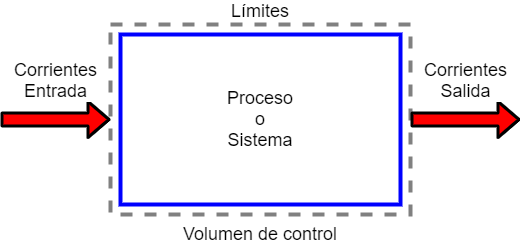
\includegraphics[width=.7\textwidth]{img/diagramas/esquema_balance_de_masa.png}
        \caption{Esquema del balance de masa sobre un volumen de control de límites definidos}
        \label{fig:bm_esquema}
    \end{figure}
    
    \begin{equation}
    \label{eq:bm_general}
        \begin{matrix}
            \text{Entrada} - \text{Salida} + & \underbrace{\text{Generación} - \text{Consumo}} & = \text{Acumulación} \\
              & \text{Reacción química} & 
        \end{matrix}
    \end{equation}
    
        \subsubsection{Proceso Estacionario}
        
        Todas las variables del proceso son independientes del tiempo (\(T\), \(P\), \(F\), \(X_{i}\), \(\cdot\)).
        
        \[
        \begin{matrix}
                \text{Entrada} - \text{Salida} + & \underbrace{\text{Generación} - \text{Consumo}} & = \cancelto{0}{\text{Acumulación}} \\
                  & \text{Reacción química} & 
        \end{matrix}
        \]
        \begin{equation}
        \label{eq:bm_estacionario}
            \text{Salida} - \text{Entrada} = \text{Generación} - \text{Consumo}
        \end{equation}
        
        \subsubsection{Con reacción}
        
            \subsubsubsection{Reactivo Limitante}
            
            \[a A + b B \rightarrow c C\]
            
            \(N_{A0}, N_{B0}\): número de moles iniciales de \(A\) y \(B\).
            
            \begin{itemize}
                \item Reacción en condiciones estequiométricas:
                \[\frac{N_{A0}}{N_{B0}} = \frac{a}{b}; \frac{N_{A0}}{a} = \frac{N_{B0}}{b}\]
                
                \item Reacción en condiciones \underline{no} estequiométricas:
                \[\frac{N_{A0}}{N_{B0}} \neq \frac{a}{b}\]
                
                Existe un reactivo limitante y un reactivo en exceso
            \end{itemize}
            
            \[\frac{N_{A0}}{N_{B0}} > \frac{a}{b} \Rightarrow A \text{: reactivo en exceso } \wedge B \text{: reactivo limitante}\]
            \[\frac{N_{A0}}{N_{B0}} < \frac{a}{b} \Rightarrow A \text{: reactivo limitante } \wedge B \text{: reactivo en exceso}\]
            
            \subsubsubsection{Conceptos}
            
            \textbf{Conversión (\(X_{A}\))}:
            
            \begin{quote}
                \textit{\say{Es la fracción del reactivo (\(A\)) que reacciona}}
            \end{quote}
            
            \[X_{A} = \frac{\text{moles de reactivo A que reaccionan}}{\text{moles iniciales de reactivo A}} = \frac{N_{A0} - N_{Af}}{N_{A0}}\]
            
            \textbf{Exceso (\(e\))}:
            
            \begin{equation}
             \label{eq:exceso}
                \begin{matrix}
                    e = \frac{N - N_{d}}{N_{d}} &  & \% e = \frac{N - N_{d}}{N_{d}} \cdot 100
                \end{matrix}
            \end{equation}
            
            \(N\): Cantidad presente del reactivo en exceso.
            
            \(N_{d}\): Cantidad estequiométrica requerida según el reactivo limitante.
            
            \subsubsubsection{Grado de avance}
            
            Velocidad de formación de \(C\):
            
            \[r_{c} = \frac{1}{V}\frac{dN_{C}}{dt}\]
            \begin{equation}
            \label{eq:grado_avance}
                \dot{\xi} = \frac{r_{A}}{-a} = \frac{r_{B}}{-b} = \frac{r_{C}}{c}
            \end{equation}
            
            \[
            \begin{matrix}
                r_{A} = -a \dot{\xi} & & r_{B} = -b \dot{\xi} & & r_{C} = c \dot{\xi}
            \end{matrix}
            \]
        
            \subsubsubsection{Balance diferencial}
            
            \textbf{Global}:
            \begin{equation}
            \label{eq:bm_rxn_global_diff}
                \frac{dm}{dt} = \sum_{j \text{ entra}} \dot{m}_{j} - \sum_{j \text{ sale}} \dot{m}_{j}
            \end{equation}
            
            \begin{equation}
            \label{eq:bm_rxn_global_diff_mol}
                \frac{dn}{dt} = \sum_{j \text{ entra}} \dot{n}_{j} - \sum_{j \text{ sale}} \dot{n}_{j} + \sum_{k \text{ reacciones}} \left ( \sum_{i \text{ compuestos}} \gamma_{i,k} \right ) \dot{\xi}_{k}
            \end{equation}
            
            Con \(\gamma_{i,k}\) coeficiente estequiométrico de \(i\) en la reacción \(k\) y \(\dot{\xi}_{k}\) grado de avance de la reacción \(k\).
            
            \textbf{Por especie}:
            \begin{equation}
            \label{eq:bm_rxn_sp_diff}
                \frac{d{m}_{i}}{dt} = \sum_{j \text{ entra}} \dot{m}_{i,j} - \sum_{j \text{ sale}} \dot{m}_{i,j} + \sum_{k \text{ reacciones}} M_{i}\gamma_{i,k}\dot{\xi}_{k}
            \end{equation}
            \begin{equation}
            \label{eq:bm_rxn_sp_diff_mol}
                \frac{d{n}_{i}}{dt} = \sum_{j \text{ entra}} \dot{n}_{i,j} - \sum_{j \text{ sale}} \dot{n}_{i,j} + \sum_{k \text{ reacciones}} \gamma_{i,k} \dot{\xi}_{k}
            \end{equation}
            
            Con \(M_{i}\) peso molecular de \(i\).
            
            \subsubsubsection{Balance integral}
            
            \textbf{Global}:
            \begin{equation}
            \label{eq:bm_rxn_global_int}
                m_{f} - m_{0} = \sum_{j \text{ entra}} \left ( \int_{t_{0}}^{t_{f}} \dot{m}_{j} dt \right ) - \sum_{j \text{ sale}} \left ( \int_{t_{0}}^{t_{f}} \dot{m}_{j} dt \right )
            \end{equation}
            \begin{equation}
            \label{eq:bm_rxn_global_int_mol}
                n_{f} - n_{0} = \sum_{j \text{ entra}} \left ( \int_{t_{0}}^{t_{f}} \dot{n}_{j} dt \right ) - \sum_{j \text{ sale}} \left ( \int_{t_{0}}^{t_{f}} \dot{n}_{j} dt \right ) + \sum_{k \text{ reacciones}} \sum_{i \text{ compuestos}} \left ( \int_{t_{0}}^{t_{f}} \gamma_{i,k} \dot{\xi}_{k} dt \right )
            \end{equation}
            
            \textbf{Por especie}:
            \begin{equation}
            \label{eq:bm_rxn_sp_int}
                m_{i,f} - m_{i,0} = \sum_{j \text{ entra}} \left ( \int_{t_{0}}^{t_{f}} \dot{m}_{i,j} dt \right ) - \sum_{j \text{ sale}} \left ( \int_{t_{0}}^{t_{f}} \dot{m}_{i,j} dt \right )  + \sum_{k \text{ reacciones}} \left ( \int_{t_{0}}^{t_{f}} M_{i} \gamma_{i,k} \dot{\xi}_{k} dt \right )
            \end{equation}
            \begin{equation}
            \label{eq:bm_rxn_sp_int_mol}
                n_{i,f} - n_{i,0} = \sum_{j \text{ entra}} \left ( \int_{t_{0}}^{t_{f}} \dot{n}_{i,j} dt \right ) - \sum_{j \text{ sale}} \left ( \int_{t_{0}}^{t_{f}} \dot{n}_{i,j} dt \right )  + \sum_{k \text{ reacciones}} \left ( \int_{t_{0}}^{t_{f}} \gamma_{i,k} \dot{\xi}_{k} dt \right )
            \end{equation}
    
    \subsection{Velocidad de reacción}
    
        \subsubsection{Orden de la reacción}
        
        \[A + B \rightarrow \text{productos}\]
        
        \textbf{Velocidad de desaparición de \(A\)}:
        
        \[
        \begin{matrix}
            -r_{A} = f \left ( T, C_{i} \right ) & & - r_{A} = k(T)f \left ( C_{A}, C_{B} \right )
        \end{matrix}
        \]
        
        \begin{multicols}{2}
            \(k_{A}\): constante (coeficiente) cinética.
        
            \(C_{A}, C_{B}\): concentraciones
        \end{multicols}
        
        \textbf{Orden de la reacción}:
        \[-r_{A} = k_{A} C_{A}^{\alpha} C_{B}^{\beta}\]
        
        \begin{multicols}{3}
            \(\alpha\): Orden respecto de \(A\)
        
            \(\beta\): Orden respecto de \(B\)
            
            \(n = \alpha + \beta\): Orden global
        \end{multicols}
        
        \begin{quote}
            \textit{\say{El orden de las reacciones se determina experimentalmente.}}
        \end{quote}
        
        \begin{quote}
            \textit{\say{Cuando los exponentes de los términos de concentración corresponden a las coeficientes estequiométricos de la reacción, usualmente se dice que las \textbf{reacciones} son \textbf{elementales}.}}
        \end{quote}
        
        \[
        \begin{matrix}
            aA + bB \rightarrow \text{productos} & & -r_{A} = k_{A}C_{A}^{a}C_{B}^{b}
        \end{matrix}
        \]
        
            \begin{multicols}{2}
                \subsubsubsection{Orden cero}
            
                \begin{equation}
                \label{eq:orden_cero}
                    -r_{A} = k_{A}
                \end{equation}
                
                \subsubsubsection{Primer orden}
                
                \begin{equation}
                \label{eq:primer_orden}
                    -r_{A} = k_{A}C_{A}
                \end{equation}
            \end{multicols}
            
            \subsubsubsection{Segundo orden}
            
            \begin{equation}
            \label{eq:segundo_orden}
                -r_{A} = k_{A} C_{A}^{2} \vee -r_{A} = k_{A} C_{A} C_{B}
            \end{equation}
            
        \subsubsection{Reacciones reversibles}
        
        Para reacciones homogéneas elementales reversibles:
        
        \[aA + bB \underset{k_{-1}}{\overset{k_{1}}{\leftrightharpoons}} cC + dD\]
        
        Velocidad de reacción de A:
        
        \begin{equation}
        \label{eq:reaccion_reversible}
            \begin{matrix}
                -r_{\text{directa}} = k_{1}C_{A}^{a}C_{B}^{b} & & r_{\text{inversa}} = k_{-1}C_{C}^{c}C_{D}^{d}
            \end{matrix}
        \end{equation}
        
        En equilibrio dinámico:
        
        \[r_{\text{directa}} + r_{\text{inversa}} = 0 \Rightarrow\]
        \[k_{1}C_{Ae}^{a}C_{Be}^{b} = k_{-1}C_{Ce}^{c}C_{De}^{d} \Rightarrow\]
        \begin{equation}
        \label{eq:contantes_reversibles}
            K_{C} = \frac{k_{-1}C_{Ce}^{c}C_{De}^{d}}{C_{Ae}^{a}C_{Be}^{b}} = \frac{k_{1}}{k_{-1}}
        \end{equation}
        
        Con \(K_{C}\) constante de equilibrio.
    
        \subsubsection{Efecto de la temperatura}
        
        Efecto de la temperatura en la velocidad de la reacción
        
        \[A \rightarrow \text{productos}\]
        
        \begin{equation}
        \label{eq:velocidad_vs_temperatura}
            -r_{A} = \frac{1}{V}\frac{dN_{A}}{dt} = k\left ( T \right ) f \left ( C \right )
        \end{equation}
        
        Con \(N_{A}\) moles de \(A\), \(V\) volumen de reacción y \(C\) concentraciones. \(k\) depende de la temperatura (es independiente de la concentración).
            
            \begin{itemize}
                \item Reacción exotérmica (\textbf{Figura \ref{fig:energia_activacion}.a}): \(E_{\text{reactantes}} > E_{\text{productos}}\)
                \item Reacción endotérmica (\textbf{Figura \ref{fig:energia_activacion}.b}): \(E_{\text{reactantes}} < E_{\text{productos}}\)
            \end{itemize}
            
            \begin{figure}
                \centering
                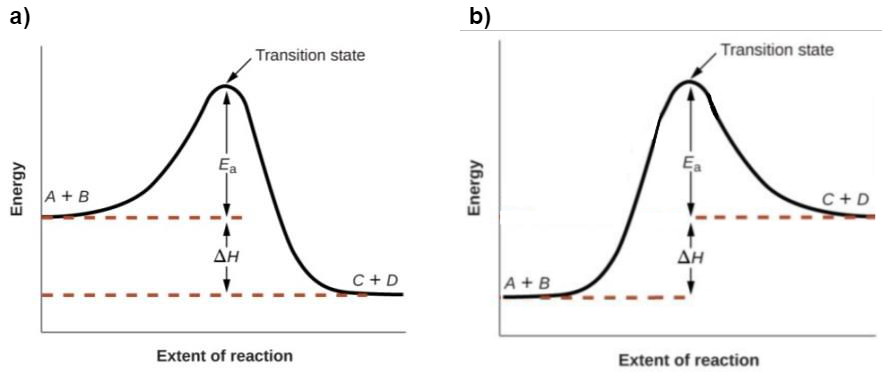
\includegraphics[width=\textwidth]{img/graficos/energia_activacion.png}
                \caption[Diagrama de la Energía de activación de una reacción]{Diagrama de la Energía de activación de una reacción. \textbf{a)} Reacción exotérmica. \textbf{b)} Reacción endotérmica}
                \label{fig:energia_activacion}
            \end{figure}
            
            \subsubsubsection{Ecuación de Arrhenius}
            
            \begin{equation}
            \label{eq:arrhenius}
                k\left ( T \right ) = A e^{\left ( \frac{-E_{a}}{RT} \right )}
            \end{equation}
            
            Con \(A\) factor de frecuencia, \(E_{A}\) energía de activación, \(R\) constante de los gases y \(T\) temperatura absoluta (en \([K]\) o \([R]\))
            
            \begin{figure}
                \centering
                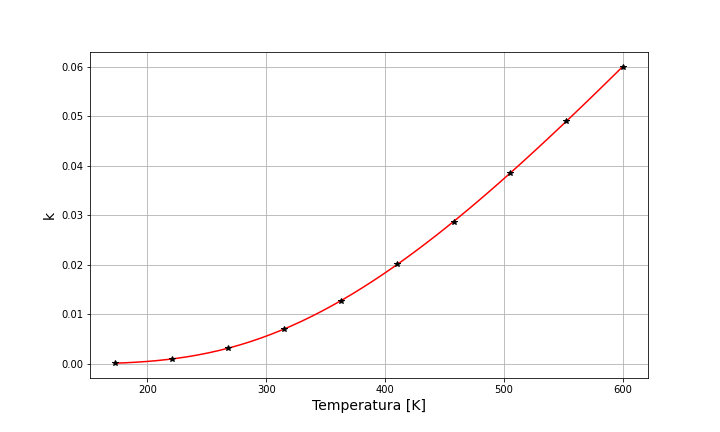
\includegraphics[width=.7\textwidth]{img/graficos/arrhenius_exp.png}
                \caption{Dependencia de la constante de velocidad con la temperatura absoluta}
                \label{fig:arrhenius_exp}
            \end{figure}
            
            Linealizando la ecuación de Arrhenius (\textbf{Ecuación \ref{eq:arrhenius}}):
            
            \[\overset{/ \ln({})}{\Rightarrow} \ln({k}) = \ln({A\cdot e^{\left ( \frac{-E_{a}}{RT} \right )}})\]
            \[\Rightarrow \ln({k}) = \ln({A}) + \frac{-E_{a}}{RT}\]
            
            \begin{equation}
            \label{eq:arrhenius_lineal}
                \ln({k}) = \ln({A}) - \frac{E_{a}}{R} \left ( \frac{1}{T} \right )
            \end{equation}
            
            \begin{figure}
                \centering
                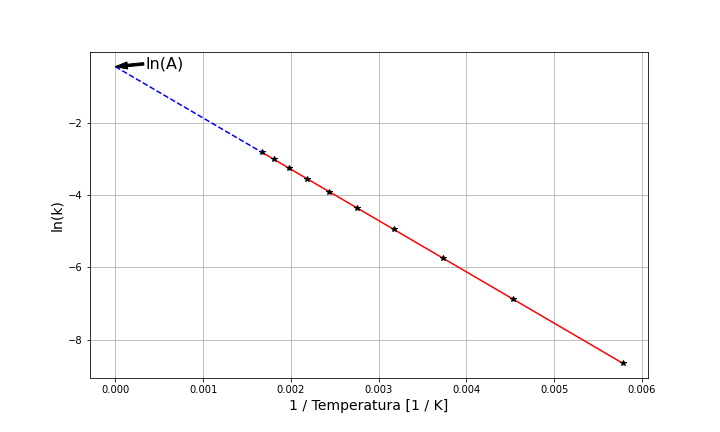
\includegraphics[width=.7\textwidth]{img/graficos/arrhenius_lineal.png}
                \caption{Ecuación linealizada de Arrhenius}
                \label{fig:arrhenius_lineal}
            \end{figure}
            
            En la \textbf{Figura \ref{fig:arrhenius_lineal}} se muestra como obtener el factor de frecuencia \(A\) extrapolando los datos obtenidos cuando \(T \rightarrow \infty \Rightarrow \frac{1}{T} \rightarrow 0\), con la pendiente igual a \(\frac{-E_{a}}{R}\) como se muestra en la \textbf{Ecuación \ref{eq:arrhenius_lineal}}.
            
            Comparando la misma reacción a temperaturas \(T_{1}\) a \(T_{2}\)
            
            \[
            \begin{matrix}
                k\left ( T_{1} \right ) = k_{T_{1}} = A e^{\left ( \frac{-E_{a}}{RT_{1}} \right )} & & k\left ( T_{2} \right ) = k_{T_{2}} = A e^{\left ( \frac{-E_{a}}{RT_{2}} \right )}
            \end{matrix} \overset{\text{Dividiendo }k_{T_{1}}\text{ por }k_{T_{2}}}{\Rightarrow}
            \]
            \[\frac{k_{T_{1}}}{k_{T_{2}}} = \frac{\cancel{A} e^{\left ( \frac{-E_{a}}{RT_{1}} \right )}}{\cancel{A} e^{\left ( \frac{-E_{a}}{RT_{2}} \right )}} \Rightarrow\]
            \[\frac{k_{T_{1}}}{k_{T_{2}}} = e^{\left ( \frac{-E_{a}}{R}\frac{1}{T_{1}} - \frac{-E_{a}}{R}\frac{1}{T_{2}} \right )} \Rightarrow\]
            
            \begin{equation}
            \label{eq:arrhenius_comparada}
                \frac{k_{T_{1}}}{k_{T_{2}}} = e^{\frac{-E_{a}}{R} \left (\frac{1}{T_{1}} - \frac{1}{T_{2}} \right )}
            \end{equation}

\section{Tipo de reactores}
    
Modalidad de operación:

\begin{enumerate}
    \begin{minipage}{0.3\linewidth}
        \item Lote (o Batch)
    \end{minipage}
    \begin{minipage}{0.3\linewidth}
        \item Continuo
    \end{minipage}
    \begin{minipage}{0.3\linewidth}
        \item Semicontinuo (o semibatch)
    \end{minipage}
\end{enumerate}

\begin{table}[H]
    \resizebox{\textwidth}{!}{
        \begin{tabular}{|l|ll|ll|}
            \hline
            \textbf{Fases}                                            & \multicolumn{2}{l|}{}                                   & \multicolumn{2}{l|}{\textbf{Reactor/modalidad}}                                              \\ \hline
            \multicolumn{1}{|c|}{\multirow{3}{*}{\textbf{Homogéneo}}} & \multicolumn{2}{l|}{\multirow{3}{*}{}}                  & \multicolumn{2}{l|}{Lote (Batch)}                                                   \\
            \multicolumn{1}{|c|}{}                           & \multicolumn{2}{l|}{}                                   & \multirow{2}{*}{Continuo:} & \begin{tabular}[c]{@{}l@{}} \textbullet tanque agitado\\ (CSTR: \textit{continuous stirred tank reactor})\end{tabular} \\
            \multicolumn{1}{|c|}{}                           & \multicolumn{2}{l|}{}                                   &                            & \begin{tabular}[c]{@{}l@{}} \textbullet flujo pistón\\ (PFR: \textit{plug-flow reactor})\end{tabular}                  \\ \hline
            \multirow{5}{*}{\textbf{Heterogéneo}}                     & \multirow{2}{*}{No-Catalítico} & Gas-sólido             & \multicolumn{2}{l|}{Lecho fijo, lecho fluidizado}                                   \\
                                                             &                                & Gas-líquido            & \multicolumn{2}{l|}{CSTR, columna de burbujeo}                                      \\ \cline{2-5} 
                                                             & \multirow{3}{*}{Catalítico}    & Gas-catalítico         & \multicolumn{2}{l|}{Lecho fijo, lecho fluidizado}                                   \\
                                                             &                                & Líquido.catalítico     & \multicolumn{2}{l|}{Lecho fijo, lecho fluidizado}                                   \\
                                                             &                                & Gas-líquido-catalítico & \multicolumn{2}{l|}{Lecho fijo con burbujeo, lecho fluidizado, ...}                 \\ \hline
        \end{tabular}
    }
    \caption{Reactores químicos}
    \label{tab:reactores_quimicos}
\end{table}

\textbf{Ejemplos}:
    
\begin{multicols}{2}
    \begin{itemize}
        \item Tanque agitado: Batch o CSTR (\textbf{Figura \ref{fig:reactor_batch}, \ref{fig:reactor_agitado_batch}, \ref{fig:reactor_cstr}})
        \item Flujo pistón: continuo (\textbf{Figura \ref{fig:reactor_flujo_piston}, \ref{fig:reactor_columna_rellena}})
        \item Columna burbujeo (\textbf{Figura \ref{fig:reactor_burbujeo}})
        \item Lecho fluidizado (\textbf{Figura \ref{fig:reactor_lecho_fluidizado}})
    \end{itemize}
    
    \begin{figure}
        \centering
        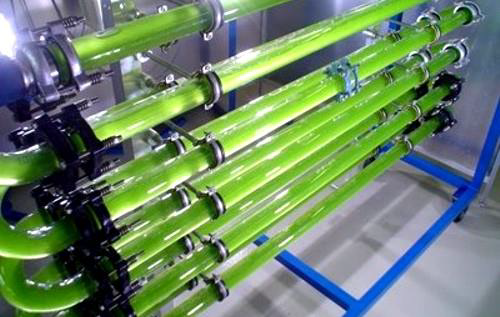
\includegraphics[width=\textwidth]{img/fotos/biorreactor_flujo_piston.png}
        \caption{Ejemplo de reactor de flujo pistón continuo, producción de biodiésel de algas}
        \label{fig:reactor_flujo_piston}
    \end{figure}
    
    \begin{figure}
        \centering
        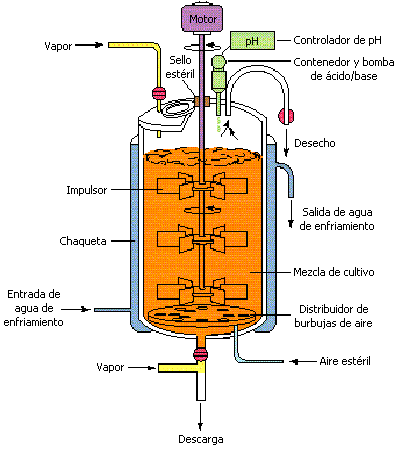
\includegraphics[width=\textwidth]{img/esquemas/reactor_batch.png}
        \caption{Esquema de tanque agitado en Batch}
        \label{fig:reactor_batch}
    \end{figure}

    \begin{figure}
        \centering
        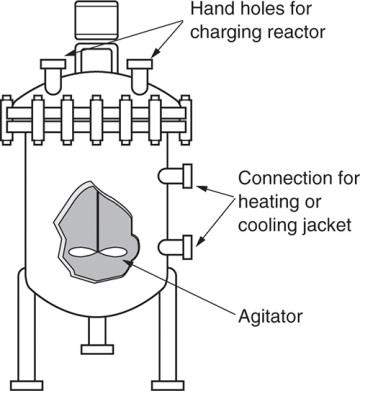
\includegraphics[width=\textwidth]{img/esquemas/reactor_agitado_batch.png}
        \caption{Reactor agitado por lote (Batch)}
        \label{fig:reactor_agitado_batch}
    \end{figure}
    
    \begin{figure}
        \centering
        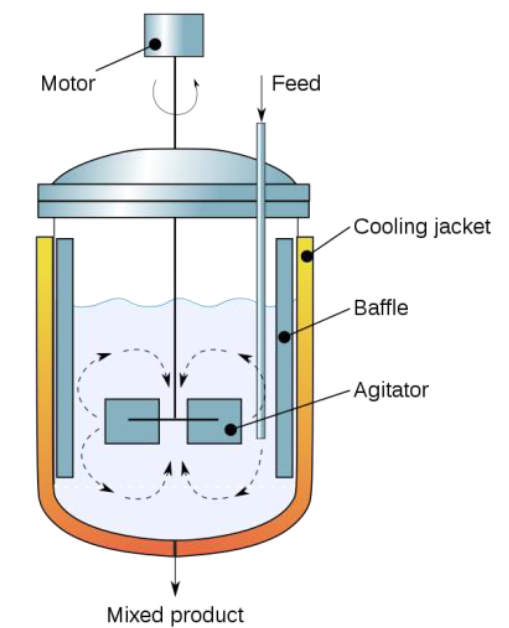
\includegraphics[width=\textwidth]{img/esquemas/reactor_cstr.png}
        \caption{Reactor agitado, continuo (CSTR)}
        \label{fig:reactor_cstr}
    \end{figure}
\end{multicols}

\begin{multicols}{3}
    \begin{figure}
        \centering
        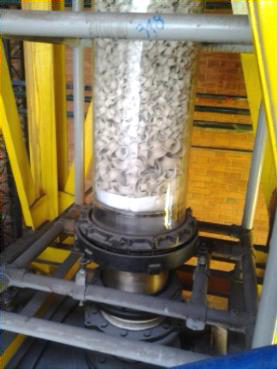
\includegraphics[width=\textwidth]{img/fotos/reactor_columna_rellena.png}
        \caption{Columna rellena (lecho fijo)}
        \label{fig:reactor_columna_rellena}
    \end{figure}
    
    \begin{figure}
        \centering
        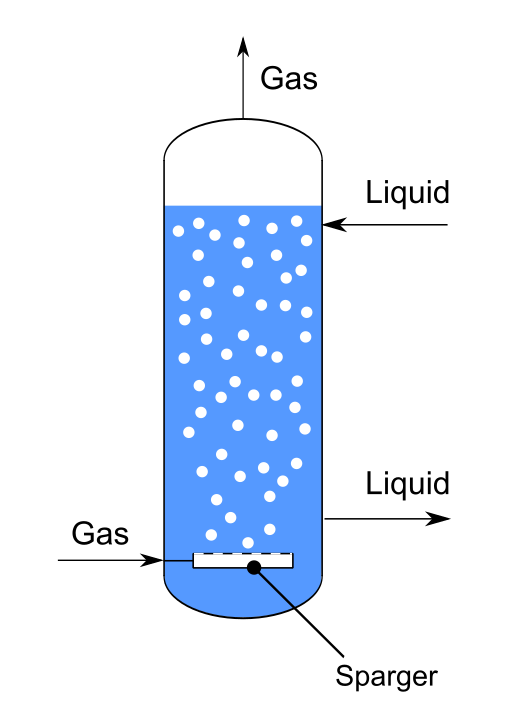
\includegraphics[width=\textwidth]{img/esquemas/reactor_burbujeo.png}
        \caption{Burbujeo}
        \label{fig:reactor_burbujeo}
    \end{figure}
    
    \begin{figure}
        \centering
        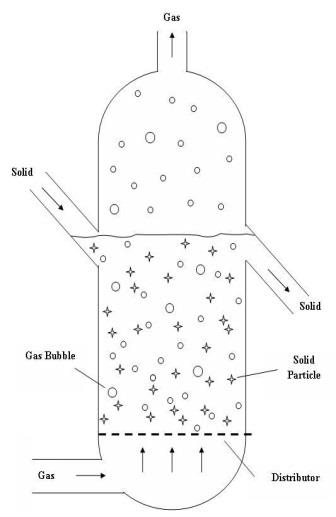
\includegraphics[width=\textwidth]{img/esquemas/reactor_lecho_fluidizado.png}
        \caption{Lecho fluidizado}
        \label{fig:reactor_lecho_fluidizado}
    \end{figure}
\end{multicols}
    
    \subsection{Reactor por lote (Batch) isotérmico}
    
    Proceso homogéneo y discontinuo (\textbf{Tabla \ref{tab:reactores_quimicos}}). Reactor perfectamente agitado (mezcla completa) (\textbf{Figura \ref{fig:reactor_agitado_batch}}).
    
        \subsubsection{Sistema a volumen y presión constante}
        
        \[V = cte\]
        
        Con \(V\) volumen del fluido (reacción).
        
        Balance de masa de \(i\) (\textbf{Ecuación \ref{eq:bm_general}}):
        
        \[\cancelto{0}{\text{Entrada}} - \cancelto{0}{\text{Salida}} + \underbrace{\text{Generación} - \text{Consumo}} = \text{Acumulación} \Rightarrow\]
        \[\int r_{i} dV = \frac{dN_{i}}{dt} \overset{\text{Mezcla perfecta}}{\Rightarrow}\]
        \[r_{i}V = \frac{d\cancelto{C_{i}V}{N_{i}}}{dt} = \frac{dC_{i}V}{dt} = V \frac{dC_{i}}{dt} + C_{i} \cancelto{0}{\frac{dV}{dt}}\]
        \begin{equation}
        \label{eq:batch_v_cte}
            r_{i} = \frac{dC_{i}}{dt}
        \end{equation}
        
        Para gases ideales:
        \[r_{i} = \frac{dC_{i}}{dt} \overset{PV = nRT}{\Rightarrow} \;\; \overset{P_{i} = C_{i}RT}{\Rightarrow}\]
        
        \begin{equation}
        \label{eq:batch_v_cte_gas_ideal}
            r_{i} = \frac{1}{RT} \frac{dP_{i}}{dt}
        \end{equation}
        
        Con \(P_{i}\) la presión parcial de \(i\).
        
        \subsubsection{Tiempo de operación}
        
        Procesos en el reactor:
        
        \begin{multicols}{2}
            \begin{enumerate}
                \item Carga de reactivos
                \item Reacción
                \item Descarga de producto(s)
                \item Limpieza
            \end{enumerate}
        \end{multicols}
        
        \[\text{tiempo total de operación} = \text{tiempo reacción} + \text{tiempos muertos}\]
        
        \begin{equation}
        \label{eq:batch_tiempo_op}
            t_{op} = t_{rxn} + t_{muerto}
        \end{equation}
        
        Con \(t_{muerto}\), los tiempos de carga, descarga, limpieza, etc.
        
        \subsubsection{Determinación del tiempo de reacción}
        
        Sea \(A\), el reactivo limitante:
        \begin{equation}
        \label{eq:r_a_n_a}
            r_{A} = \frac{1}{V} \frac{dN_{A}}{dt}
        \end{equation}
        \[\Rightarrow dt = \frac{d N_{A}}{r_{A}V} \overset{\int}{\Rightarrow}\]
        
        Con límites \(t = 0 \Rightarrow N_{A}(t=0) = N_{A0}\) y \(t = t \Rightarrow N_{A}(t=t) = N_{A}\):
        
        \[\int_{0}^{t} dt = \int_{N_{A0}}^{N_{A}} \frac{d N_{A}}{r_{A}V} \Rightarrow\]
        
        \begin{equation}
        \label{eq:tiempo_rxn_batch_intermedio}
            t = \int_{N_{A0}}^{N_{A}} \frac{d N_{A}}{r_{A}V}
        \end{equation}
        
        Sea \(X_{A}\) la conversión del reactivo \(A\):
        \[N_{A} = N_{A0} \left ( 1 - X_{A} \right ) \overset{\text{Reemplazando en \textbf{Ecuación \ref{eq:r_a_n_a}}}}{\Rightarrow}\]
        \[r_{A} = \frac{1}{V} \frac{d\left ( N_{A0} \left ( 1 - X_{A} \right ) \right ) }{dt} \]
        
        Resolviendo la derivada:
        \[d\left ( N_{A0} \left ( 1 - X_{A} \right ) \right ) = d\left ( N_{A0} - N_{A0} X_{A} \right ) \overset{N_{A0}=cte}{=} \cancelto{0}{d \left ( N_{A0} \right )} - N_{A0} dX_{A}\]
        
        Realizando mismo procedimiento anterior:
        \[r_{A} = \frac{1}{V} \frac{- N_{A0} dX_{A}}{dt} \Rightarrow \]
        \[dt = \frac{- N_{A0} dX_{A}}{r_{A} V} \overset{\int}{\Rightarrow} \]
        
        Con límites \(t = 0 \Rightarrow X_{A}(t=0) = 0\) y \(t = t \Rightarrow X_{A}(t=t) = X_{A}\):
        
        \begin{equation}
        \label{eq:volumen_batch}
            t = N_{A0} \int_{0}^{X_{A}} - \frac{d X_{A}}{r_{A}V}
        \end{equation}
        
        Y como \(C_{A} = \frac{N_{A}}{V}\):
        
        \begin{equation}
        \label{eq:tiempo_rxn_batch_conc}
            t = C_{A0} \int_{0}^{X_{A}} - \frac{d X_{A}}{r_{A}}
        \end{equation}
        
        \subsubsection{Volumen y Presión variable}
        
        \[r_{A} = \frac{1}{V} \frac{dN_{A}}{dt}\]
        
            \subsubsubsection{Fase líquida}
            
            \[
            \begin{matrix}
                \rho \text{ (densidad)} & = & cte & \rightarrow & V & = & cte \\
                \rho & \neq & cte & \rightarrow & V & = & f(X)
            \end{matrix}
            \]
            
            \subsubsubsection{Fase gaseosa}
            
            Volumen dependerá de la estequiometría de la reacción
            \[\Delta N_{T} = \left ( \sum N_{\text{productos}} - \sum N_{\text{reactantes}} \right )\]
            \[
            \begin{matrix}
                \text{Si } & \Delta N_{T} = 0 & \rightarrow & V = cte \\
                \text{Si } & \Delta N_{T} \neq 0 & \rightarrow & 
                \begin{matrix}
                    \left ( V = cte \wedge P \neq cte \right ) & \vee \\
                    \left ( V \neq cte \wedge P = cte \right ) & 
                \end{matrix}
            \end{matrix}
            \]
            
            Gas ideal:
            \[PV = N_{T}RT \Rightarrow V = \frac{N_{T}RT}{P} \overset{/ V_{0}}{\Rightarrow}\]
            \begin{equation}
            \label{eq:razones_volumen}
                \frac{V}{V_{0}} = \left ( \frac{N_{T}}{N_{T0}} \right ) \left ( \frac{T}{T_{0}} \right ) \left ( \frac{P_{0}}{P} \right )
            \end{equation}
            
            \textbf{Coeficiente de expansión (\(\varepsilon\))}:
            
            \begin{quote}
                \textit{\say{Razón entre la variación en el total de moles para una conversión completa y los moles totales iniciales.}}
            \end{quote}
            
            \begin{equation}
            \label{eq:coef_expansion}
                \varepsilon = \frac{N_{Tf} - N_{T0}}{N_{T0}}
            \end{equation}
            
            \[N_{T} = N_{T0} \left ( 1 + \varepsilon X \right )\]
            
            Con \(X\) la conversión.
            \newline
            
            \textbf{Presión variable}:
            
            De la \textbf{Ecuación \ref{eq:razones_volumen}} a volumen y temperatura constante:
            
            \[\cancelto{1}{\frac{V}{V_{0}}} = \frac{N_{T}}{N_{T0}}\cancelto{1}{\frac{T}{T_{0}}}\frac{P_{0}}{P}\]
            \begin{equation}
            \label{eq:batch_presion_var}
                \left ( \frac{P}{P_{0}} \right ) = \left ( \frac{N_{T}}{N_{T0}} \right )
            \end{equation}
            \newpage
            
            \textbf{Volumen variable}:
            
            De la \textbf{Ecuación \ref{eq:razones_volumen}} a presión y temperatura constante:
            
            \[\frac{V}{V_{0}} = \frac{N_{T}}{N_{T0}}\cancelto{1}{\frac{T}{T_{0}}}\cancelto{1}{\frac{P_{0}}{P}}\]
            \[\left ( \frac{V}{V_{0}} \right ) = \left ( \frac{N_{T}}{N_{T0}} \right )\]
            \[\overset{N_{T} = N_{T0} \left ( 1 + \varepsilon X \right )}{\Rightarrow} \left ( \frac{V}{V_{0}} \right ) = \left ( \frac{\cancel{N_{T0}} \left ( 1 + \varepsilon X \right )}{\cancel{N_{T0}}} \right )\]
            \begin{equation}
            \label{eq:batch_volumen_var}
                V = V_{0} \left ( 1 + \varepsilon X \right )
            \end{equation}
            
            \begin{quote}
                \textit{\say{El volumen varía linealmente con la conversión.}}
            \end{quote}
            
            Con tiempo de reacción:
            
            \[r_{A} = \frac{1}{V} \frac{dN_{A}}{dt} \Rightarrow\]
            \[r_{A} = \frac{1}{V} \frac{- N_{A0} dX_{A}}{dt} \overset{\text{\textbf{Ecuación \ref{eq:batch_volumen_var}}}}{\Rightarrow}\]
            \[r_{A} = \frac{1}{V_{0} \left ( 1 + \varepsilon X_{A} \right )} \frac{- N_{A0} dX_{A}}{dt} \overset{\int}{\Rightarrow}\]
            
            \begin{equation}
            \label{eq:tiempo_rxn_batch_conc_conv}
                t = C_{A0} \int_{0}^{X_{A}} - \frac{d X_{A}}{r_{A} \left ( 1 + \varepsilon X_{A} \right )}
            \end{equation}
        
        \subsubsection{Reactores Agitados}
        
        ¿Para qué agitar? (\textbf{Figura \ref{fig:reactor_agitado_batch}}).
        
        \begin{multicols}{2}
            \begin{itemize}
                \item Mezclar dos fluidos miscible (ej. alcohol y agua)
                \item Disolución de sólidos en líquidos (ej. sal en agua)
                \item Mejorar la transferencia de calor (calentamiento o enfriamiento)
                \item Dispersión de un gas en un líquido (Ej. aire u oxígeno en un caldo de fermentación)
                \item Mejorar la transferencia de masa
            \end{itemize}
        \end{multicols}
        
            \subsubsubsection{Dimensiones del reactor}
            
            \begin{figure}
                \centering
                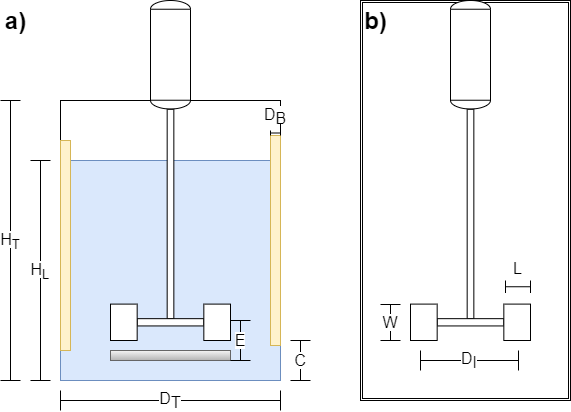
\includegraphics[width=.7\textwidth]{img/diagramas/Dimensiones Reactor Agitado.png}
                \caption[Dimensiones reactor agitado]{Dimensiones reactor agitado. \textbf{a)} Dimensiones del reactor, donde \(H_{T}\) es la altura total del reactor, \(H_{L}\) es la altura del líquido, \(D_{B}\) ancho del deflector o \textit{baffle}, \(E\) distancia entre el impulsor y el difusor de aire (en caso de biorreactores), \(C\) la holgura y \(D_{T}\) diámetro total del reactor. \textbf{b)} Dimensiones de la turbina, con \(D_{I}\) diámetro del impulsor, \(W\) ancho del impulsor y \(L\) el ancho de la cuchilla (\textit{blade}).}
                \label{fig:dimensiones_reactor_agitado}
            \end{figure}
            
            \begin{multicols}{2}
                \begin{table}[H]
                    \resizebox{\textwidth}{!}{
                        \begin{threeparttable}
                            \begin{tabular}{|c|rcl|}
                                \hline
                                \(\nicefrac{H_{L}}{H_{T}}\) & \(0.7\) & \(-\) & \(0.8\) \\
                                \(\nicefrac{H_{T}}{D_{T}}\) & \(1.0\) & \(-\) & \(2.0\) \\
                                \(\nicefrac{H_{L}}{D_{T}}\) & \(0.5\) & \(-\) & \(1.5\) (típico \(1.0\)) \\
                                \(\nicefrac{D_{B}}{D_{T}}\) & \(0.08\) & \(-\) & \(0.12\) \\
                                \(\nicefrac{D_{T}}{D_{I}}\) & \(2.0\) & \(-\) & \(3.0\) \\
                                \(\nicefrac{D_{I}}{W}\) &  & \(5.0\)* &  \\
                                \(\nicefrac{D_{I}}{L}\) &  & \(4.0\)* &  \\
                                \hline
                            \end{tabular}
                            \begin{tablenotes}
                                \item (*) Usando una Turbina Rushton (\textbf{Figura \ref{fig:turbina_rushton}}) como ejemplo.
                            \end{tablenotes}
                            \caption[Razones típicas entre dimensiones de un reactor agitado]{Razones típicas entre dimensiones de un reactor agitado. Medidas en la \textbf{Figura \ref{fig:dimensiones_reactor_agitado}}}
                            \label{tab:dimensiones_reactor_agitado}
                        \end{threeparttable}
                    }
                \end{table}
                
                \begin{figure}
                    \centering
                    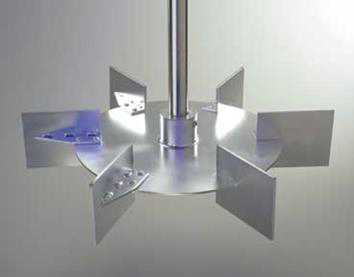
\includegraphics[width=\textwidth]{img/fotos/turbina_rushton.png}
                    \caption{Turbina Rushton}
                    \label{fig:turbina_rushton}
                \end{figure}
            \end{multicols}
            \newpage
            
            \subsubsubsection{Tipos de Agitadores}
            
            \begin{multicols}{2}
                \begin{figure}
                    \centering
                    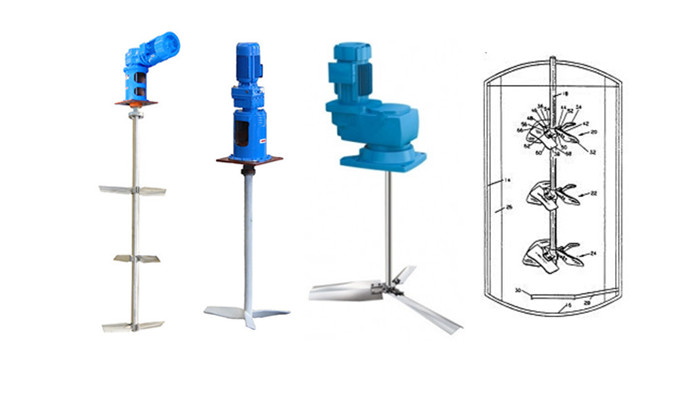
\includegraphics[width=\textwidth]{img/fotos/batch_agitado_entrada_por_arriba.jpg}
                    \caption[Agitador con Entrada por Arriba]{Agitador con Entrada por Arriba \cite{cd_agitatorcom_cd_2012}}
                    \label{fig:batch_agitado_entrada_por_arriba}
                \end{figure}
                \begin{figure}
                    \centering
                    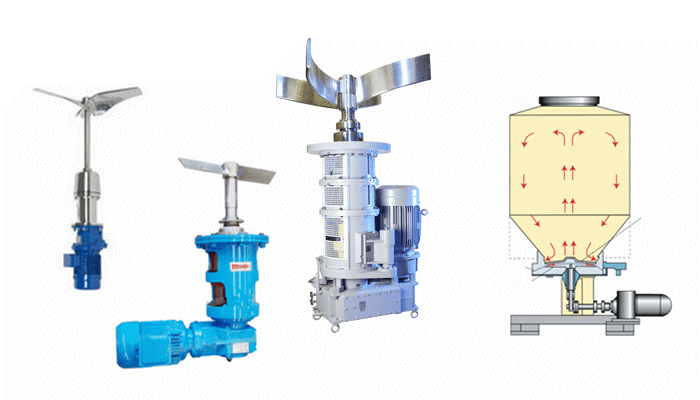
\includegraphics[width=\textwidth]{img/fotos/batch_agitado_entrada_por_abajo.png}
                    \caption[Agitador con Entrada por Abajo]{Agitador con Entrada por Abajo \cite{cd_agitatorcom_cd_2012}}
                    \label{fig:batch_agitado_entrada_por_abajo}
                \end{figure}
            \end{multicols}
            
            \begin{figure}
                \centering
                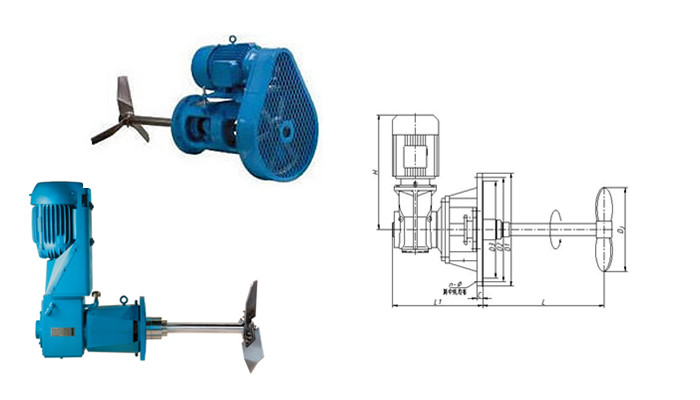
\includegraphics[width=.5\textwidth]{img/fotos/batch_agitado_entrada_por_lado.jpg}
                \caption[Agitador con Entrada por el Lado]{Agitador con Entrada por el Lado \cite{cd_agitatorcom_cd_2012}}
                \label{fig:batch_agitado_entrada_por_lado}
            \end{figure}
            
            \begin{figure}
                \centering
                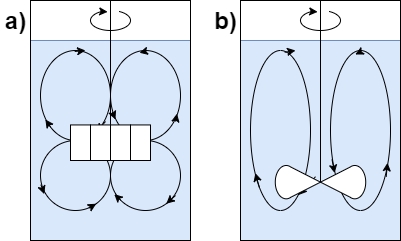
\includegraphics[width=.6\textwidth]{img/diagramas/Agitadores Flujos.png}
                \caption[Tipos de flujos generados por agitador]{Tipos de flujos generados por agitador. \textbf{a)} Flujo radial. \textbf{b)} Flujo axial.}
                \label{fig:agitadores_tipos_flujos}
            \end{figure}
            
            \begin{figure}
                \centering
                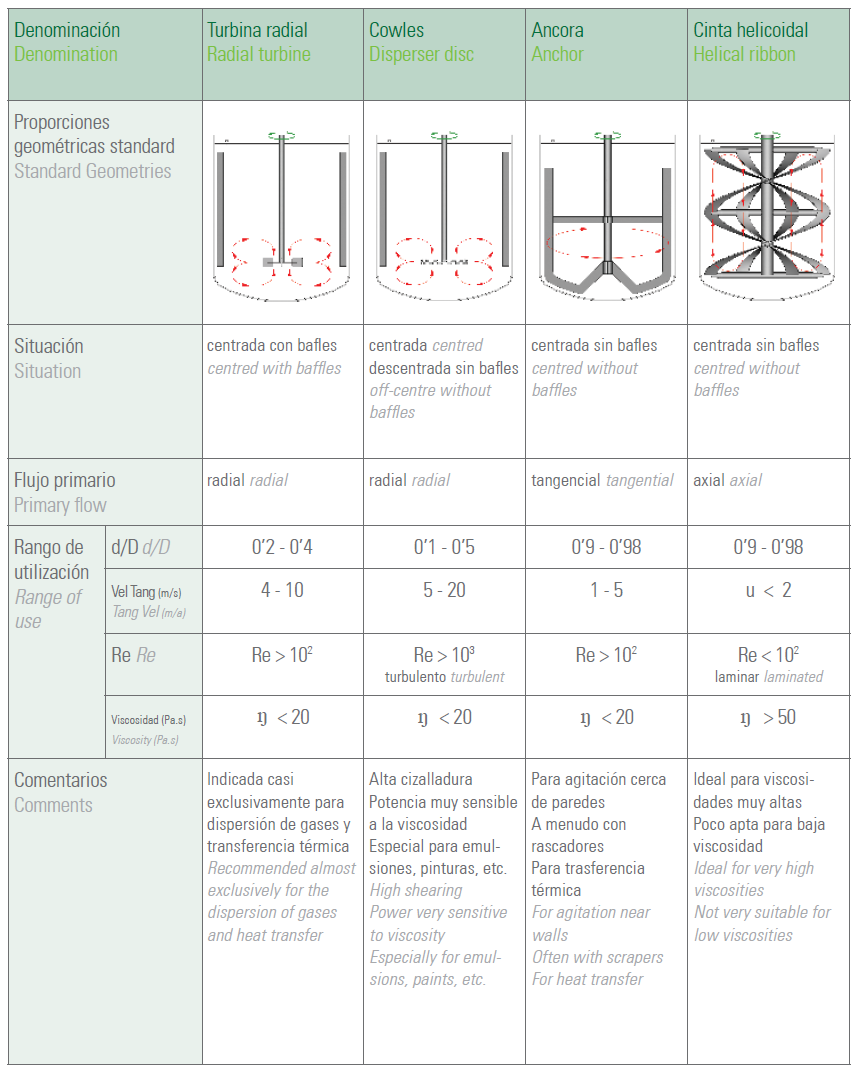
\includegraphics[width=\textwidth]{img/esquemas/resumen_impulsores_cont.png}
                \caption[Tabla resumen de impulsores]{Tabla resumen de impulsores. Continúa en \textbf{Figura \ref{fig:impulsores_resumen_cont}}}
                \label{fig:impulsores_resumen}
            \end{figure}
            
            \begin{figure}
                \centering
                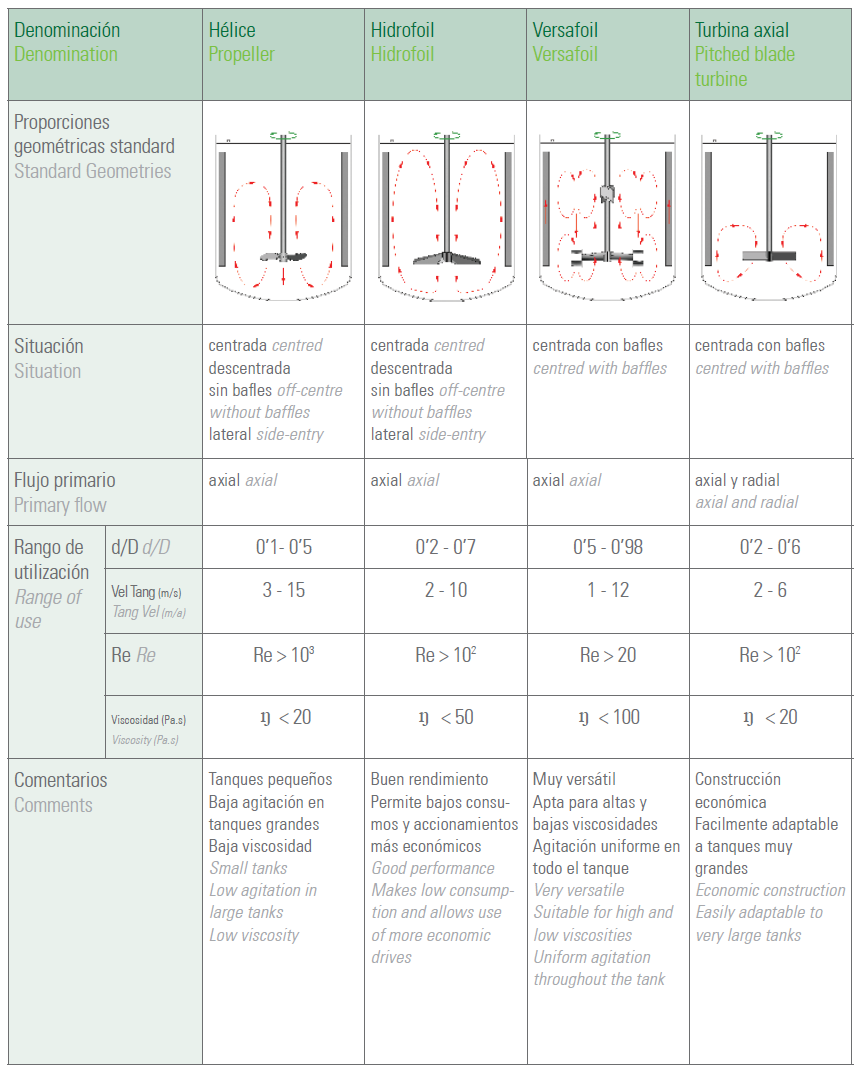
\includegraphics[width=\textwidth]{img/esquemas/resumen_impulsores.png}
                \caption[Tabla resumen de impulsores (continuación)]{Tabla resumen de impulsores. Continuación de \textbf{Figura \ref{fig:impulsores_resumen}}}
                \label{fig:impulsores_resumen_cont}
            \end{figure}
            
            \begin{figure}
                \centering
                \includegraphics[width=.9\textwidth]{img/esquemas/Impulsores.png}
                \caption{Diferentes flujos producidos por diferentes tipos de impulsores}
                \label{fig:impulsores}
            \end{figure}
            
            \subsubsubsection{Cálculo de Potencia}
            
            La potencia requerida para el mezclamiento depende de:
            
            \begin{multicols}{2}
                \begin{itemize}
                    \item Velocidad de agitación
                    \item Geometría y tamaño del impulsor
                    \item Geometría del reactor
                    \item Densidad y viscosidad del flujo
                \end{itemize}
            \end{multicols}
            
            Uso de números adimensionales.
            
            \begin{multicols}{2}
                \textbf{Número de Reynolds}:
                
                \begin{equation}
                \label{eq:numero_reynolds}
                    {Re}_{i} = \frac{N_{i}{D_{i}}^{2}\rho}{\mu}
                \end{equation}
                
                Con \(N_{i}\) velocidad (angular) del agitados, \(D_{i}\) diametro del impulsor, \(\rho\) densidad del fluido y \(\mu\) viscosidad.
                
                \textbf{Número de potencia}:
                
                \begin{equation}
                \label{eq:numero_potencia}
                    {N}_{P} = \frac{P}{\rho {N_{i}}^{3}{D_{i}}^{5}}
                \end{equation}
                
                Con \(N_{P}\) número de potencia y \(P\) potencia.
                \newline
                \newline
            \end{multicols}    
                
            \textbf{Cálculo de potencia}:
            
            \begin{equation}
            \label{eq:calculo_potencia}
                P = {N}_{P}\rho {N_{i}}^{3}{D_{i}}^{5}
            \end{equation}
            
            \begin{figure}
                \centering
                \includegraphics[height=.94\textheight]{img/esquemas/Re_Np.png}
                \caption[Correlación entre el número de potencia y el número de Reynolds]{Correlación entre el número de potencia y el número de Reynolds para \textbf{(1)} Turbina Rushton (\textbf{Figura \ref{fig:resumen_impulsores}.a}), \textbf{(2)} Paleta (\textbf{Figura \ref{fig:resumen_impulsores}.b}) y \textbf{(3)} Hélice Marina (\textbf{Figura \ref{fig:resumen_impulsores}.c}) \cite{doran_bioprocess_2004}}
                \label{fig:Re_Np}
            \end{figure}
            
            \begin{figure}
                \centering
                \includegraphics[width=.5\textwidth]{img/fotos/Resumen Impulsores.png}
                \caption[Impulsores de agitación]{Impulsores de agitación usados en la \textbf{Figura \ref{fig:Re_Np}}. \textbf{a)} Turbina Rushton. \textbf{b)} Paleta. \textbf{c)} Hélice Marina.}
                \label{fig:resumen_impulsores}
            \end{figure}
            
            \textbf{Flujo laminar}:
            
            Como se muestra en el gráfico de la \textbf{Figura \ref{fig:Re_Np}}, \(N_{P}\) es inversamente proporcional a \({Re}_{i}\):
            \[N_{P} \propto \frac{1}{{Re}_{i}} \Rightarrow N_{P} = \frac{k_{1}}{{Re}_{i}}\]
            \[\overset{\text{\textbf{Ecuación \ref{eq:numero_potencia}}}}{\Rightarrow} \frac{P}{\rho {N_{i}}^{3}{D_{i}}^{5}} = \frac{k_{1}}{{Re}_{i}}\]
            \[\overset{\text{\textbf{Ecuación \ref{eq:numero_reynolds}}}}{\Rightarrow} \frac{P}{{\cancelto{1}{\rho}} {N_{i}}^{\cancelto{2}{3}} {D_{i}}^{\cancelto{3}{5}}} = \frac{k_{1} \mu}{{\cancelto{1}{N_{i}}}{{\cancelto{1}{D_{i}^{2}}}}{\cancelto{1}{\rho}}} \Rightarrow\]
            \begin{equation}
            \label{eq:flujo_laminar}
                P = k_{1} \mu {N_{i}}^{2} {D_{i}}^{3}
            \end{equation}
            
            \begin{multicols}{2}
                \textbf{Flujo turbulento}:
            
                Como se muestra en el gráfico de la \textbf{Figura \ref{fig:Re_Np}}, \(N_{P}\) se vuelve constante:
                
                \[N_{P} = cte = {N'}_{P}\overset{\text{\textbf{Ecuación \ref{eq:numero_potencia}}}}{\Rightarrow}\]
                \begin{equation}
                \label{eq:flujo_turbulento}
                    P = {{N'}}_{P}\rho {N_{i}}^{3}{D_{i}}^{5}
                \end{equation}
                
                \begin{figure}
                    \centering
                    \includegraphics[width=\textwidth]{img/esquemas/k1_np_impulsores.png}
                    \caption{Diferentes valores de \(k_{1}\) y \({N'}_{P}\) para diferentes tipos de impulsores}
                    \label{fig:k1_np_impulsores}
                \end{figure}
            \end{multicols}

    \subsection{Reactor continuo perfectamente agitado (CSTR) isotérmico}
    
    \begin{minipage}{0.3\linewidth}
        \begin{figure}
            \centering
            \includegraphics[width=\textwidth]{img/diagramas/esquema_cstr.png}
            \caption{Esquema simple de CSTR}
            \label{fig:esquema_CSTR}
        \end{figure}
    \end{minipage}
    \begin{minipage}{0.6\linewidth}
        Reactores Continuos Ideales:
        
        \begin{itemize}
            \item \textbf{Reactor continuo perfectamente agitado (\textit{Continuous Stirred Tank Reactor}, CSTR)}
            \item Reactor continuo flujo pistón (\textit{Plug Flow Reactor}, PFR)
        \end{itemize}
    \end{minipage}
    
    \textbf{Características}:
    
    \begin{itemize}
        \item Flujo continuo de reactantes y productos
        \item Opera en Estado Estacionario
        \item Mezcla perfecta
        \item La composición del flujo de salida es igual a la composición dentro del reactor
    \end{itemize}
    
    La mayoría de los reactores continuos de \underline{fase líquida} homogénea son CSTR.
    
    \begin{multicols}{2}
        \textbf{Ventajas}:
    
        \begin{itemize}
            \item Operación continua
            \item Producto de calidad constante
            \item Buen control de temperatura
            \item Menores tiempos muertos, respecto de un reactor por lote (batch)
            \item Más fácil limpieza, comparado con un reactor fljo pistón (PFR)
            \item Adaptable a operaciones de más de una fase
        \end{itemize}
        
        \textbf{Desventajas}
        
        \begin{itemize}
            \item Baja conversión por unidad de volumen (comparado con otros reactores continuos)
            \item Mayor costo de inversión que reactor Batch (requiere equipos auxiliares, bombas)
            \item Posibles desviaciones respecto del flujo ideal
            \item []
            \item []
        \end{itemize}
    \end{multicols}
    
    \begin{table}[H]
        \centering
        \resizebox{\textwidth}{!}{
            \begin{tabular}{|l|cc|}
                \hline
                                                                                                                    & \textbf{Lote (Batch)}     & \textbf{Continuo (CSTR)}                                                            \\ \hline
                \rowcolor[HTML]{C0C0C0} 
                \textbf{Bajos volúmenes de producción}                                                              & Ventaja                   &                                                                                     \\
                \textbf{\begin{tabular}[c]{@{}l@{}}Largas corridas de producción,\\ grandes volúmenes\end{tabular}} &                           & Ventaja                                                                             \\
                \rowcolor[HTML]{C0C0C0} 
                \textbf{Calidad del producto}                                                                       & Puede ser variable        & Uniforme (constante)                                                                \\
                \textbf{Flexibilidad (multipropósito)}                                                              & Ventaja                   &                                                                                     \\
                \rowcolor[HTML]{C0C0C0} 
                \textbf{Costo de capital}                                                                           & Bajo                      & Alto                                                                                \\
                \textbf{Tiempos muertos}                                                                            & Desventaja                &                                                                                     \\
                \rowcolor[HTML]{C0C0C0} 
                \textbf{\begin{tabular}[c]{@{}l@{}}Procesamiento aguas abajo \\ (\textit{downstream})\end{tabular}}          & Requiere estanques pulmón & \begin{tabular}[c]{@{}c@{}}Ventaja si las otras\\ etapas son continuas\end{tabular} \\ \hline
            \end{tabular}
        }
        \caption{Comparación entre reactor por Batch y CSTR}
        \label{tab:comparacion_batch_cstr}
    \end{table}
    
        \subsubsection{Reactor continuo}
        
        De la \textbf{Ecuación \ref{eq:bm_general}}, en \textbf{\underline{estado estacionario}}:
        
        \[
        \begin{matrix}
            \text{Entrada} - \text{Salida} + \text{Generación} - \text{Consumo} = \cancelto{0}{\text{Acumulación}}
        \end{matrix}
        \]
        
        \begin{figure}
            \centering
            \includegraphics[width=.7\textwidth]{img/diagramas/esquema_reactor_continuo.png}
            \caption{Esquema de un reactor continuo}
            \label{fig:reactor_continuo}
        \end{figure}
        
        Por lo tanto:
        
        \[F_{A0}-F_{A}-X_{A}\cdot F_{A0} \overset{\text{Estado Estacionario}}{=} 0 \Rightarrow\]
        
        \begin{equation}
        \label{eq:reactor_continuo}
            F_{A} = F_{A0} \left ( 1 - X_{A} \right ) \text{, con } F_{A0} = C_{A0}\cdot v_{0} \wedge F_{A} = C_{A}\cdot v_{S}
        \end{equation}
        
        Con \(F_{A0}\) flujo molar de \(A\) en la entrada en \(\left [ \frac{mol\;A}{t} \right ]\) (\textbf{Figura \ref{fig:reactor_continuo}}), \(C_{A0}\) concentración molar de \(A\) en la entrada, \(X_{A}\) conversión de \(A\) en \(\left [ \frac{mol\;A \text{ que reaccionan}}{mol\;A \text{ que entran}} \right ]\) y \(v_{0}\) flujo volumétrico de entrada.
        
        \subsubsection{Reactor continuo perfectamente agitado isotérmico}
        
        Tenemos que, para gases ideales:
        
        \[C_{A0} = \frac{P_{A0}}{R{T}_{0}} = \frac{y_{A0}P_{0}}{R{T}_{0}}\]
        
        Con \(y_{A0}\) fracción molar de \(A\) en la entrada, \(P_{0}\) presión total de entrada, \(P_{A0}\) presión parcial de \(A\) a la entrada, \(R\) constante de los gases y \(T_{0}\) temperatura absoluta a la entrada.
        
        Sea \(r_{A}\) la tasa de reacción de \(A\), en estado estacionario se tiene:
        
        \[F_{A0} - F_{A} + r_{A} V = 0 \Rightarrow F_{A} = r_{A} V + F_{A0}\]
        
        De la \textbf{Ecuación \ref{eq:reactor_continuo}}
        
        \[F_{A} = F_{A0} \left ( 1 - X_{A} \right ) \overset{F_{A} = r_{A} V + F_{A0}}{\Rightarrow}\]
        \[r_{A} V + F_{A0} = F_{A0} \left ( 1 - X_{A} \right ) \Rightarrow\]
        \[-r_{A} V = \cancel{F_{A0}} - F_{A0} \left ( \cancel{1} - X_{A} \right ) \Rightarrow\]
        \begin{equation}
        \label{eq:volumen_cstr}
            V = \frac{F_{A0} X_{A}}{-r_{A}}
        \end{equation}
        
        \textit{Nota}: A veces \(X_{A}\) se escribe solo \(X\) y se refiere al \textbf{reactivo limitante}.
        
            \subsubsubsection{Reacciones irreversibles}
            
            Para reacciones \underline{irreversibles} de orden mayor a cero:
            
            \[-r_{A} = k C_{A}^{n} \wedge C_{A} = C_{A0} \left ( 1 - X_{A} \right )\]
            \[\Rightarrow -r_{A} = k C_{A0}^{n} \left ( 1 - X_{A} \right )^{n}\]
            
            \begin{figure}
                \centering
                \includegraphics[width=.6\textwidth]{img/graficos/ordenes_reaccion.png}
                \caption{Comparación entre ordenes de reacción}
                \label{fig:ordenes_reac_comparacion}
            \end{figure}
            
            Cuando \(X_{A} \rightarrow 1 \text{, } -r_{A} \rightarrow 0 \Rightarrow\)
            
            \[\frac{1}{-r_{A}} \rightarrow \infty \text{, } V \rightarrow \infty\]
            
            Para reacciones \underline{irreversibles} de orden cero:
            
            \[-r_{A} = \left\{
            \begin{matrix}
                k &  & \text{si } 0 \leq X_{A} < 1 \\ 
                0 &  & \text{si } X_{A} = 1
            \end{matrix}\right.\]
            
            \[-r_{A} = k \theta \left ( 1 - X_{A} \right )\]
            
            Con \(\theta\) una función escalón, tal que:
            
            \[\theta \left ( 1 - X_{A} \right ) = \left\{
            \begin{matrix}
                1 &  & \text{si } 0 \leq X_{A} < 1 \\ 
                0 &  & \text{si } X_{A} = 1
            \end{matrix}\right.\]
            
            \begin{figure}
                \centering
                \includegraphics[width=.6\textwidth]{img/graficos/funcion_theta.png}
                \caption{Función escalón \(\theta\)}
                \label{fig:funcion_escalo_theta}
            \end{figure}
            
            De la \textbf{Ecuación \ref{eq:volumen_cstr}} reemplazando \(-r_{A}\):
            
            \[V = \frac{F_{A0} X_{A}}{k \theta \left ( 1 - X_{A} \right )}\]
            
            \begin{equation}
            \label{eq:volumen_cstr_irreversible_orden_cero}
                V = \left\{
                \begin{matrix}
                    \frac{F_{A0} X_{A}}{k} &  & \text{si } 0 \leq X_{A} < 1 \\ 
                    \rightarrow \infty &  & \text{si } X_{A} = 1
                \end{matrix}\right.
            \end{equation}
            
            \subsubsubsection{Reacciones reversibles}
            
            Para reacciones \textit{reversibles}, la conversión máxima es la de equilibrio (\(X_{Ae}\)). Cuando \(X_{A} \rightarrow X_{Ae}\text{, }-r_{A} \rightarrow 0 \Rightarrow\)
            \[\frac{1}{-r_{A}} \rightarrow \infty \text{, } V \rightarrow \infty\]
            
            Para una reacción:
            \[
            \begin{matrix}
                 & k_{\overset{\rightarrow}{A}} & \\
                A + \cdots & \rightleftharpoons & \cdots \\
                 & k_{\overset{\leftarrow}{A}} &
            \end{matrix}
            \]
            \[-r_{A} = r_{\overset{\rightarrow}{A}} - r_{\overset{\leftarrow}{A}}\]
            \[-r_{A} = k_{\overset{\rightarrow}{A}} C_{A0}^{n}\left(1 - X_{A}\right )^{n} (\cdots) - k_{\overset{\leftarrow}{A}} C_{A0}^{n}{X_{A}}^{n} (\cdots)\]
            
            
            \subsubsubsection{Estado estacionario}
        
            Como en estado estacionario:
            
            \[F_{A0} - F_{A} + r_{A} V = 0 \overset{\text{Usando las definiciones de } F_{A0} \text{ y } F_{A} \text{ de la \textbf{Ecuación \ref{eq:reactor_continuo}}}}{\Rightarrow}\]
            \begin{equation}
            \label{eq:reactor_continuo_concentracion}
                C_{A0}\cdot v_{0} - C_{A} \cdot v_{S} + r_{A} V = 0
            \end{equation}
        
            \subsubsubsection{Sistemas líquidos}
        
            En sistemas líquidos con densidad constante:
            
            \[v_{0} = v_{S} = v\]
            \begin{equation}
            \label{eq:reactor_continuo_concentracion_densidad_cte}
                \left ( C_{A0} - C_{A} \right ) \cdot v + r_{A}\cdot V = 0
            \end{equation}
            
            \subsubsubsection{Sistemas gaseosos}
        
            Para gases ideales:
            
            \[PV = nRT \Rightarrow C_{T} = \frac{P}{RT}\]
            
            Con \(C_{T}\) concentración molar total en el gas.
            
            Si \(F_{T}\) es el flujo total en el gas y \(v\) flujo volumétrico del gas:
            
            \[C_{T} = \frac{F_{T}}{v} \overset{\text{Gases ideales}}{=} \frac{P}{RT}\]
            
            Y para la entrada del reactor:
            
            \[C_{T0} = \frac{F_{T0}}{v_{0}} = \frac{P_{0}}{R{T}_{0}}\]
            
            Despejando el flujo volumétrico (\(v\) y \(v_{0}\)) en ambas:
            
            \[v = \frac{{F}_{T} RT}{P} \wedge v_{0} = \frac{{F}_{T0} R{T}_{0}}{{P}_{0}}\]
            
            Entonces:
            
            \begin{equation}
            \label{eq:reactor_cont_flujo_vol}
                v = v_{0} \left ( \frac{{F}_{T}}{F_{T0}} \right ) \left ( \frac{T}{{T}_{0}} \right ) \left ( \frac{{P}_{0}}{P} \right )
            \end{equation}
            
            Si \(\varepsilon \neq 0 \rightarrow\) existe variación del flujo volumétrico:
            
            \[F_{T} = F_{T0} \left ( 1 + \varepsilon X_{A} \right )\]
            
            \begin{equation}
            \label{eq:reactor_cont_flujo_vol_var}
                v = v_{0} \left ( 1 + \varepsilon X_{A} \right ) \left ( \frac{T}{{T}_{0}} \right ) \left ( \frac{{P}_{0}}{P} \right )
            \end{equation}
            
            Si \(P\) y \(T\) son constantes:
            
            \begin{equation}
            \label{eq:reactor_cont_flujo_vol_var_pt_cte}
                v = v_{0} \left ( 1 + \varepsilon X_{A} \right )
            \end{equation}
            
            \subsubsubsection{Tiempo de residencia (o tiempo espacial) (\(\tau\))}
            
            \begin{quote}
                \textit{\say{Tiempo necesario para procesar el volumen de entrada de fluido equivalente al volumen del reactor}}
            \end{quote}
            
            \begin{equation}
            \label{eq:tiempo_residencia}
                \tau = \frac{V}{v_{0}}
            \end{equation}
            
            \subsubsubsection{Velocidad espacial (\(SV\))}
            
            \begin{equation}
            \label{eq:velocidad_espacial}
                SV = \frac{v_{0}}{V} = \frac{1}{\tau}
            \end{equation}
        
    \subsection{Reactor continuo flujo pistón (PFR) isotérmico}
    
    \begin{minipage}{0.3\linewidth}
        \begin{figure}
            \centering
            \includegraphics[width=\textwidth]{img/diagramas/esquema_pfr.png}
            \caption{Esquema simple de PFR}
            \label{fig:esquema_PFR}
        \end{figure}
    \end{minipage}
    \begin{minipage}{0.6\linewidth}
        Reactores Continuos Ideales:
    
        \begin{itemize}
            \item Reactor continuo perfectamente agitado (\textit{Continuous Stirred Tank Reactor}, CSTR)
            \item \textbf{Reactor continuo flujo pistón (\textit{Plug Flow Reactor}, PFR)}
        \end{itemize}
    \end{minipage}
    \newline
    
    \textbf{Características}:
    
    \begin{itemize}
        \item Opera en estado estacionario
        \item Flujo continuo de reactantes y productos
        \item Se asume que opera en régimen turbulento
        \item No existe dispersión o difusión de flujo en el sentido axial
        \item Se asume perfectamente mezclado en el sentido radial
        \item Sin agitación
        \item Composición varía a lo largo del reactor
    \end{itemize}
    
    La mayoría de los reactores en \underline{fase gaseosa} homogénea son reactores flujo pistón (PFR).
    
    \begin{figure}
        \centering
        \includegraphics[width=.6\textwidth]{img/diagramas/esquema_reactor_flujo_piston.png}
        \caption{Esquema de un reactor flujo pistón}
        \label{fig:esquema_reactor_flujo_piston}
    \end{figure}
    
    \begin{figure}
        \centering
        \includegraphics[width=0.75\textwidth]{img/diagramas/regimen_de_movimiento.png}
        \caption[Esquema de Régimen Laminar y Turbulento)]{Esquema del régimen laminar (\textbf{a}) y turbulento (\textbf{b})}
        \label{fig:regimen_movimiento}
    \end{figure}
    
    En caso de régimen turbulento (\textbf{Figura \ref{fig:regimen_movimiento}.b}) no hay gradiente radial de temperatura, velocidad de flujo o concentración. Se modela como flujo pistón, \(\left \| Re > 4000 \right \| \)
    
    \begin{multicols}{2}
        \textbf{Ventajas}:
        
        \begin{itemize}
            \item Operación continua
            \item Altos niveles de producción
            \item Preferidos para reacciones fase gaseosa
            \item Alta conversión por unidad de volumen
        \end{itemize}
        
        \textbf{Desventajas}:
        
        \begin{itemize}
            \item Control de temperatura
            \item No es fácil de limpiar
            \item No usar cuando existen incrustaciones (\textit{fouling})
        \end{itemize}
    \end{multicols}
    
    \textbf{Recomendado}:
    \begin{multicols}{2}
        \begin{itemize}
            \item Reacciones en fase gaseosa
            \item Reacciones rápidas
            \item Régimen turbulento
            \item Niveles altos de producción
        \end{itemize}
    \end{multicols}
    
        \subsubsection{Isotérmico e Isobárico}
        
        \begin{figure}
            \centering
            \includegraphics[width=.6\textwidth]{img/diagramas/esquema_pfr_variables.png}
            \caption{Esquema de un PFR con sus variables físicas y químicas}
            \label{fig:esquema_pfr_variables}
        \end{figure}
        
        Realizando el balance de \(A\):
        \[F_{A} - \left ( F_{A} + dF_{A} \right ) + r_{A}dV \overset{\text{Estado estacionario}}{=}0\]
        \[\Rightarrow -dF_{A} = -r_{A}dV\]
        
        Por otro lado:
        \[F_{A} = F_{A0} \left (1 - X_{A} \right ) \Rightarrow dF_{A} = -F_{A0}dX_{A}\]
        
        Igualando \(dF_{A}\):
        \begin{equation}
        \label{eq:flujo_tur_cont}
            -r_{A}dV = F_{A0}dX_{A}
        \end{equation}
        
        Despejando \(dV\) de la \textbf{Ecuación \ref{eq:flujo_tur_cont}}:
        \[dV = F_{A0} \frac{dX_{A}}{-r_{A}} \overset{\int}{\Rightarrow}\]
        \[\int_{0}^{V} dV = F_{A0} \int_{X_{A0}}^{X_{Af}} \frac{dX_{A}}{-r_{A}} \Rightarrow\]
        \begin{equation}
        \label{eq:volumen_pfr}
            V = F_{A0} \int_{X_{A0}}^{X_{Af}} \frac{dX_{A}}{-r_{A}}
        \end{equation}
        
        De la definición de tiempo residencia (\textbf{Ecuación \ref{eq:tiempo_residencia}})
        \[\tau = \frac{V}{v_{0}} = \frac{\text{Volumen}}{\text{Flujo volumétrico}}\]
        
        Con \(v_{0}\) y \(V\) (\textbf{Ecuación \ref{eq:volumen_pfr}}):
        \[v_{0} = \frac{F_{A}}{C_{A0}} \wedge\]
        \[V = F_{A0} \int_{X_{A0}}^{X_{Af}} \frac{dX_{A}}{-r_{A}}\]
        
        Tenemos:
        \[\tau = \frac{V}{v_{0}} = \frac{\cancel{F_{A0}} \int_{X_{A0}}^{X_{Af}} \frac{dX_{A}}{-r_{A}}}{\frac{\cancel{F_{A}}}{C_{A0}}} \Rightarrow\]
        \begin{equation}
        \label{eq:tiempo_residencia_pfr}
            \tau = C_{A0} \int_{X_{A0}}^{X_{Af}} \frac{dX_{A}}{-r_{A}}
        \end{equation}
        
            \subsubsubsection{En reacción de primer orden}
            
            De la \textbf{Ecuación \ref{eq:primer_orden}}:
            \[-r_{A} = kC_{A}\]
            
            Reemplazando en la \textbf{Ecuación \ref{eq:flujo_tur_cont}}:
            \[-r_{A}dV = F_{A0}dX_{A} \overset{-r_{A}}{\Rightarrow}\]
            \[kC_{A}dV = F_{A0}d{X}_{A} \Rightarrow \frac{dV}{F_{A0}} = \frac{d{X}_{A}}{k{C}_{A}}\]
            
            De la definición de \(X_{1}\):
            \[X_{A} = \frac{\left ( C_{A0} - C_{A} \right )}{C_{A0}} \overset{d()}{\Rightarrow} dX_{A} = \frac{-dC_{A}}{C_{A0}}\]
            
            Reemplazando \(dX_{A}\):
            \[\frac{dV}{F_{A0}} = \frac{\frac{-dC_{A}}{C_{A0}}}{k{C}_{A}} \Rightarrow\]
            \[\frac{dV}{F_{A0}} = \frac{-dC_{A}}{k{C}_{A0}{C}_{A}} \overset{v C_{A0} = F_{A0}}{\Rightarrow}\]
            \[\frac{dV}{v \cancel{C_{A0}}} = \frac{-dC_{A}}{k\cancel{{C}_{A0}}{C}_{A}} \overset{\int}{\Rightarrow}\]
            \[\frac{V}{v} = \frac{1}{k} \int_{C_{A0}}^{C_{A}} -\frac{dC_{A}}{C_{A}}\]
            \begin{equation}
            \label{eq:tiempo_pfr_primer_orden}
                \tau = \frac{1}{k} \ln{\left ( \frac{C_{A0}}{C_{A}} \right)}
            \end{equation}
        
            \subsubsubsection{Sistemas con densidad constante}
            
            Se tiene que:
            \[X_{A} = \frac{C_{A0}-C_{A}}{C_{A0}} = 1 - \frac{C_{A}}{C_{A0}} \overset{\text{Derivando }d \left ( \right )}{\Rightarrow}\]
            \[d \left ( X_{A} \right ) = \cancelto{0}{d(1)} - d \left (\frac{C_{A}}{\cancelto{cte}{C_{A0}}} \right ) \Rightarrow\]
            \[d X_{A} = \frac{-dC_{A}}{C_{A0}}\]
            
            Reemplazando la expresión encontrada de \(dX_{A}\) en la \textbf{Ecuación \ref{eq:volumen_pfr}} queda:
            
            \[V = F_{A0} \int_{\cancelto{C_{A0}}{X_{A0}}}^{\cancelto{C_{Af}}{X_{Af}}} \frac{\left ( dX_{A} = \frac{-dC_{A}}{C_{A0}} \right )}{-r_{A}} \overset{C_{A0}=cte}{\Rightarrow}\]
            
            \begin{equation}
            \label{eq:volumen_pfr_den_cte}
                V = - \frac{F_{A0}}{C_{A0}} \int_{C_{A0}}^{C_{Af}} \frac{dC_{A}}{-r_{A}}
            \end{equation}
            
            Como \(v_{0} = \frac{F_{A0}}{C_{A0}}\) y \(\tau = \frac{V}{v_{0}}\), reemplazando ambas en \textbf{Ecuación \ref{eq:volumen_pfr_den_cte}}:
            
            \[V = - \cancelto{v_{0}}{\frac{F_{A0}}{C_{A0}}} \int_{C_{A0}}^{C_{Af}} \frac{dC_{A}}{-r_{A}} \overset{\nicefrac{.}{v_{0}}}{\Rightarrow}\]
            \begin{equation}
            \label{eq:tiempo_residencia_pfr_den_cte}
                \tau = - \int_{C_{A0}}^{C_{Af}} \frac{dC_{A}}{-r_{A}}
            \end{equation}
            
            \subsubsubsection{Reacciones gaseosas}
            
            Para reaacciones gaseosas a \(T = cte\), \(P = cte\) y \(\Delta n \neq 0 \rightarrow \epsilon \neq 0\):
            
            \[v \overset{\text{gas ideal}}{=} v_{0} \left ( \frac{Z}{Z_{0}} \right ) \left ( \frac{N_{T}}{N_{T0}} \right ) \left ( \frac{T}{T_{0}} \right ) \left ( \frac{P_{0}}{P} \right ) \overset{cte}{\Rightarrow}\]
            \[v = v_{0} \cancelto{1}{\left ( \frac{Z}{Z_{0}} \right )} \left ( \frac{N_{T}}{N_{T0}} \right ) \cancelto{1}{\left ( \frac{T}{T_{0}} \right )} \cancelto{1}{\left ( \frac{P_{0}}{P} \right )} = v_{0}\left ( \frac{N_{T}}{N_{T0}} \right ) = v_{0} \left ( 1 + \epsilon \cdot X_{A} \right )\]
            \[\text{Como } F_{A} = C_{A} \cdot v \Rightarrow\]
            \[\frac{F_{A}}{C_{A}} = v_{0} \left ( 1 + \epsilon \cdot X_{A} \right )\]
            \begin{equation}
            \label{eq:conc_pfr_gases_partial}
                C_{A} = \frac{F_{A}}{v_{0} \left ( 1 + \epsilon \cdot X_{A} \right )}
            \end{equation}
            
            Como \(F_{A} = F_{A0} \left ( 1 - X_{A} \right )\):
            \[C_{A} = \frac{F_{A}}{v_{0} \left ( 1 + \epsilon \cdot X_{A} \right )} = \cancelto{C_{A0}}{\frac{F_{A0}}{v_{0}}} \frac{\left ( 1 - X_{A} \right )}{\left ( 1 + \epsilon \cdot X_{A} \right )}\]
            \begin{equation}
            \label{eq:conc_pfr_gases}
                C_{A} = C_{A0} \frac{\left ( 1 - X_{A} \right )}{\left ( 1 + \epsilon \cdot X_{A} \right )}
            \end{equation}
            
            \subsubsubsection{Volumen de PFR}
            
            \begin{equation}
            \label{eq:volumen_cilindro}
                V = A \cdot L = \frac{\pi {D}^{2} L}{4}
            \end{equation}
            
            Con \(D\) el diámetro transversal y \(L\) el largo longitudinal.
        
\section{Asociación de reactores: serie, paralelo, reciclo}

\begin{figure}
    \centering
    \includegraphics[width=.5\textwidth]{img/diagramas/simbologia_asociacion.png}
    \caption[Simbología para asociación de reactores]{Simbología para asociación de reactores. \textbf{a)} CSTR. \textbf{b)} PFR}
    \label{fig:asoc_simbol}
\end{figure}
    
    \subsection{Comparación entre reactores}
    
    \begin{table}[H]
        \begin{tabular}{|l|ccc|}
            \hline
            Reactor            & Batch & CSTR & PFR \\ \hline
            Ecuación de Diseño & \(\displaystyle V \cdot t = N_{A0} \int_{0}^{X_{A}} \frac{d X_{A}}{-r_{A}}\) & \(\displaystyle V = \frac{F_{A0} X_{A}}{-r_{A}}\) & \(\displaystyle V = F_{A0} \int_{X_{A0}}^{X_{Af}} \frac{dX_{A}}{-r_{A}}\) \\
                               & (\ref{eq:volumen_batch}) & (\ref{eq:volumen_cstr}) & (\ref{eq:volumen_pfr}) \\ \hline
        \end{tabular}
        \caption{Tabla de Reactores}
        \label{tab:resumen_reactores}
    \end{table}
    
        \subsubsection{CRFT vs PFR}
        
        \textbf{Relación \(\nicefrac{-1}{r_{A}}\) versus \(X_{A}\) (conversión)}:
    
        Para \textbf{CSTR} se tiene la \textbf{Ecuación \ref{eq:volumen_cstr}}:
        \[V = F_{A0}\frac{X_{A}}{-r_{A}}\]
        \[\frac{V_{CSTR}}{F_{A0}} = \frac{1}{-r_{A}} \cdot X_{A}\]
        
        Para \textbf{PFR} se tiene la \textbf{Ecuación \ref{eq:volumen_pfr}}:
        \[V = F_{A0} \int_{X_{A0}}^{X_{Af}} \frac{dX_{A}}{-r_{A}}\]
        \[\frac{V_{PFR}}{F_{A0}} = \int_{X_{A0}}^{X_{Af}} \frac{1}{-r_{A}} \cdot dX_{A}\]
        
        Por lo que si graficamos \(\nicefrac{-1}{r_{A}}\) versus \(X_{A}\), obtendremos:
        
        \begin{figure}
            \centering
            \includegraphics[width=.8\textwidth]{img/graficos/comparacion_area.png}
            \caption{Gráfico \(\nicefrac{-1}{r_{A}}\) versus \(X_{A}\) de un reactor CSTR y PFR}
            \label{fig:ra_xa_cstr_pfr}
        \end{figure}
        
        \subsubsection{PFR vs Reactor Batch}
        
        \textbf{Tiempo en reacción de primer orden}:
        
        De la \textbf{Ecuación \ref{eq:tiempo_pfr_primer_orden}} del tiempo de residencia de un PFR con reacción de primer orden:
        \[\tau = \frac{1}{k} \ln{\left ( \frac{C_{0}}{C} \right)}\]
        
        Tiempo de reacción en un reactor Batch:
        
        Recordar:
        \[\frac{dC}{dt} = kC \Rightarrow dt = \frac{1}{k} \frac{dC}{C} \overset{\int}{\Rightarrow}\]
        \[t = \frac{1}{k} \ln{\left ( \frac{C_{0}}{C} \right )}\]
    
    \subsection{Reactores en Serie}
    
    \begin{figure}
        \centering
        \includegraphics[width=\textwidth]{img/diagramas/asociacion_serie.png}
        \caption[Reactores en Serie]{\textbf{a)} CSTR conectados en serie. \textbf{b)} PFR conenctados en serie}
        \label{fig:asoc_serie}
    \end{figure}
    
    \begin{figure}
        \centering
        \includegraphics[width=.5\textwidth]{img/diagramas/asociacion_cstr_pfr.png}
        \caption{Asociación en serie entre CSTR y PFR}
        \label{fig:asoc_cstr_pfr}
    \end{figure}
    
        \subsubsection{CSTR en serie}
        
        (\textbf{Figura \ref{fig:asoc_serie}.a}) Balance del reactor \(1\) (primero):
        
        \[F_{A0} - F_{A1} + r_{A1}V_{1} \overset{\text{E.E.}}{=} 0\]
        \[-r_{A1}V_{1} = F_{A0} - F_{A1}\]
        \[V_{1} = \frac{F_{A0} - F_{A1}}{-r_{A1}} \overset{F_{A1} = F_{A0} \left ( 1 - X_{1} \right )}{\Rightarrow}\]
        \[V_{1} = \frac{\cancel{F_{A0}} - F_{A0} \left ( \cancel{1} - X_{1} \right )}{-r_{A1}}\]
        \begin{equation}
        \label{eq:volumen_1_cstr_serie}
            V_{1} = \frac{F_{A0}X_{1}}{-r_{A1}}
        \end{equation}
        \[\overset{\text{Despejando }X_{1}}{\Rightarrow} X_{1} = \frac{-r_{A1}{V}_{1}}{F_{A0}}\]
        
        Por otro lado:
        \[F_{A1} = C_{A1}v \wedge F_{A0} = C_{A0} \cdot v \text{, con } v = v_{0}\]
        \[C_{A1} = C_{A0} \left ( 1 - X_{1} \right ) \overset{\text{Reemplazando con }X_{1}}{\Rightarrow}\]
        \[C_{A1} = C_{A0} \left ( 1 - \frac{-r_{A1}{V}_{1}}{F_{A0}} \right )\]
        
        Tiempo de residencia:
        \[\tau_{1} = \frac{V_{1}}{v} = \frac{C_{A0}{V}_{1}}{F_{A0}} \Rightarrow\]
        \[C_{A1} = C_{A0} - \frac{-r_{A1}\cancelto{\tau_{1}}{{C}_{A0}{V}_{1}}}{\cancel{F_{A0}}} \overset{\tau_{1}}{\Rightarrow}\]
        \[C_{A1} = C_{A0} - \left ( -r_{A1} \tau_{1} \right )\]
        
        Balance del reactor \(2\):
        \[F_{A1} - F_{A2} + r_{A2}V_{2} \overset{\text{E.E.}}{=} 0\]
        \[-r_{A2}V_{2} = F_{A1} - F_{A2}\]
        \[V_{2} = \frac{F_{A1} - F_{A2}}{-r_{A2}} = \frac{F_{A0} \left ( 1 - X_{1} \right ) - F_{A2}}{-r_{A2}}\]
        
        Por otro lado, considerando \(X_{2}\) \underline{respecto a la entrada}:
        \[F_{A2} = F_{A0} \left (1 - X_{2} \right )\]
        
        Reemplazando \(F_{A2}\):
        \[V_{2} = \frac{F_{A0} \left ( \cancel{1} - X_{1} \right ) - F_{A0} \left (\cancel{1} - X_{2} \right )}{-r_{A2}}\]
        
        \begin{equation}
        \label{eq:volumen_2_cstr_serie}
            V_{2} = \frac{F_{A0} \left ( X_{2} - X_{1} \right )}{-r_{A2}}
        \end{equation}
        
        Despejando \(X_{2}\):
        \begin{equation}
        \label{eq:conversion_2_cstr_serie}
            X_{2} = X_{1} + \frac{-r_{A2}{V}_{2}}{F_{A0}}
        \end{equation}
        
        Dado \(v = v_{0}\):
        \[C_{A2} = C_{A0} \left (1 - X_{2} \right )\]
        
        \subsubsection{PFR en serie}
        
        (\textbf{Figura \ref{fig:asoc_serie}.b}) Balance a un reactor (\(i\)):
        
        \[\left ( - r_{A} \right ) dV_{i} = F_{A0i} dX_{i} \Rightarrow V_{i} = F_{A0i} \int_{0}^{X_{if}} \frac{dX_{i}}{-r_{A}}\]
        \[\Rightarrow \frac{V_{i}}{F_{A0i}} = \int_{0}^{X_{if}} \frac{dX_{i}}{-r_{A}}\]
        
        Para \(V = V_{1} + V_{2} + \cdots V_{n}\)
        \[\frac{V}{F_{A0}} = \sum_{i=1}^{n} \frac{V_{i}}{F_{A0}} = \frac{V_{1} + V_{2} + \cdots V_{n}}{F_{A0}} \overset{\frac{V_{i}}{F_{A0i}} = \int_{0}^{X_{if}} \frac{dX_{i}}{-r_{A}}}{\Rightarrow}\]
        \[\frac{V}{F_{A0}} = \int_{X_{0}=0}^{X_{1}} \frac{dX}{-r_{A}} + \int_{X_{1}}^{X_{2}} \frac{dX}{-r_{A}} + \cdot + \int_{X_{n-1}}^{X_{n}} \frac{dX}{-r_{A}}\]
        \begin{equation}
        \label{eq:volumen_pfr_serie}
            \frac{V}{F_{A0}} = \int_{X_{0}=0}^{X_{n}} \frac{dX}{-r_{A}}
        \end{equation}

    \subsection{Reactores en Paralelo}
    
    \begin{figure}
        \centering
        \includegraphics[width=.7\textwidth]{img/diagramas/asociacion_paralelo.png}
        \caption[Reactores en Paralelo]{\textbf{a)} CSTR conectados en paralelo. \textbf{b)} PFR conenctados en paralelo}
        \label{fig:asoc_paralelo}
    \end{figure}
    
        \subsubsection{CSTR en paralelo}
        
        (\textbf{Figura \ref{fig:asoc_paralelo}.a}) Balance a un reactor (\(i\)):
        
        \[F_{A0i} - F_{Ai} + r_{Ai}V_{i} = 0 \Rightarrow - r_{Ai}V_{i} = F_{A0i} - F_{Ai} \Rightarrow\]
        \[V_{i} = \frac{F_{A0i} - F_{Ai}}{-r_{Ai}}\]
        
        Recordar:
        \[F_{Ai} = F_{A0i} \left ( 1 - X_{Ai} \right )\]
        
        Reemplzando \(F_{Ai}\):
        \[V_{i} = \frac{ \cancel{F_{A0i}} - F_{A0i} \left ( \cancel{1} - X_{Ai} \right ) }{-r_{Ai}}\]
        \begin{equation}
        \label{eq:volumen_cstr_paralelo}
            V_{i} = \frac{F_{A0i} X_{i}}{-r_{Ai}}
        \end{equation}
        
        Si los reactores son de igual volumen y el flujo de entrada se distribuye equitativamente:
        \[V_{1} = V_{2} = \cdots = V_{n}\]
        \[X_{1} = X_{2} = \cdots = X_{n}\]
        \[C_{A1} = C_{A2} = \cdots = C_{An}\]
        \[-r_{A1} = -r_{A2} = \cdots = -r_{An}\]
        \[V_{i} = \frac{V}{n} \wedge F_{A0i} = \frac{F_{A0}}{n} \Rightarrow\]
        \[V_{i} = \frac{V}{\cancel{n}} = \frac{F_{A0}}{\cancel{n}} \cdot \frac{X_{i}}{-r_{Ai}}\]
        
        \begin{equation}
        \label{eq:volumen_total_cstr_paralelo}
            V = \frac{F_{A0}X_{i}}{-r_{Ai}} = \frac{F_{A0}X}{-r_{A}}
        \end{equation}
        
        \begin{quote}
            \textit{\say{La conversión es la misma obtenida por un solo reactor de volumen \(V\) (\(=n{V}_{i}\))}}
        \end{quote}
        
        \subsubsection{PFR en paralelo}
        
        (\textbf{Figura \ref{fig:asoc_paralelo}.b}) Balance a un reactor (\(i\)):
        
        \[\left ( - r_{A} \right ) dV_{i} = F_{A0i} dX_{i} \Rightarrow V_{i} = F_{A0i} \int_{0}^{X_{if}} \frac{dX_{i}}{-r_{A}}\]
        
        Si se desea que la conversión en ambos reactores sea la misma (La concentración de entrada a ambos reactores es la misma):
        
        \[C_{A0} = C_{A01} = C_{A02} \Rightarrow \frac{V_{1}}{F_{A01}} = \frac{V_{2}}{F_{A02}} \Rightarrow \frac{V_{1}}{V_{2}} = \frac{F_{A01}}{F_{A02}}\]
        
        De la definición de tiempo de residencia (\textbf{Ecuación \ref{eq:tiempo_residencia}}):
        \[\tau_{1} = \frac{V_{1}}{v_{01}} \wedge \tau_{2} = \frac{V_{2}}{v_{02}}\]
        
        La concentración de entrada a ambos reactores es la misma:
        \[F_{A01} = C_{A0}\cdot v_{01} \wedge F_{A02} = C_{A0}\cdot v_{02}\]
        
        Con esto tenemos:
        \[\frac{V_{1}}{V_{2}} = \frac{F_{A01}}{F_{A02}} \overset{C_{A0}\cdot v_{0}}{=} \frac{\cancel{C_{A0}}\cdot v_{01}}{\cancel{C_{A0}}\cdot v_{02}} \Rightarrow\]
        \[\frac{V_{1}}{V_{2}} = \frac{v_{01}}{v_{02}} \Rightarrow \frac{V_{1}}{v_{01}} = \frac{V_{2}}{v_{02}}\]
        \begin{equation}
        \label{pfr_paralelo_tau_equiv}
            \tau_{1} = \tau_{2}
        \end{equation}
    
    \subsection{Reactores con Reciclo}
    
    \begin{figure}
        \centering
        \includegraphics[width=.5\textwidth]{img/diagramas/asociacion_reciclo.png}
        \caption[Reactores con recirculación]{\textbf{a)} CSTR con recirculación. \textbf{b)} PFR con recirculación}
        \label{fig:asoc_reciclo}
    \end{figure}
    
    \textbf{Aplicaciones}:
    
    \begin{enumerate}
        \item Reacciones autocatalíticas.
        \item Ayuda a mantener condiciones isotermas.
        \item Cuando se requiere una alta conversión de alguno de los compuestos (ej. Eliminación de un contaminante o cumpuesto tóxico).
        \item En aplicaciones biológicas para mantener concentraciones altas de células.
    \end{enumerate}
    
    Para una reacción en fase gaseosa:
    
    \[aA + bB \rightarrow cC + dD \overset{\text{Sea }a\text{ reactivo limitante}}{\Rightarrow}\]
    \[A + \frac{b}{a}B \rightarrow \frac{c}{a}C + \frac{d}{a}D\]
    
    \begin{figure}
        \centering
        \includegraphics[width=.6\textwidth]{img/diagramas/esquema_balance_reciclo.png}
        \caption{Esquema de los flujos y volúmenes en un reactor con reciclo}
        \label{fig:balance_reciclo}
    \end{figure}
    
    \textbf{Conversión por pasada} (Figura \ref{fig:balance_reciclo}):
    
    \begin{equation}
    \label{eq:conversion_por_pasada}
        X_{p} = \frac{N_{A} \text{ que reaccionaron en una sola pasada por el reactor}}{N_{A} \text{ a la entrada del reactor}} = \frac{N_{A1} - N_{A2}}{N_{A1}}
    \end{equation}
    
    \textbf{Conversión global} (Figura \ref{fig:balance_reciclo}):
    
    \begin{equation}
    \label{eq:conversion_global}
        X_{G} = \frac{N_{A} \text{ que reaccionaron en el sistema}}{N_{A} \text{ a la entrada del sistema}} = \frac{N_{A0} - N_{A3}}{N_{A0}}
    \end{equation}
    
    \textbf{Factor de recirculación} (Figura \ref{fig:balance_reciclo}):
    
    \begin{equation}
    \label{eq:factor_recirculacion}
        R = \frac{F_{AR}}{F_{A3}} = \frac{F_{BR}}{F_{B3}} = \frac{F_{CR}}{F_{C3}} = \frac{F_{DR}}{F_{D3}}
    \end{equation}
    
    Si \(R\) (\textbf{Ecuación \ref{eq:factor_recirculacion}}):
    \begin{itemize}
        \item \( \rightarrow 0 \Rightarrow \) No existe reciclo.
        \item \( \rightarrow \infty \Rightarrow \) Se comportará como un \textbf{CSTR}.
    \end{itemize}
    
    \[\therefore \left \| R \in \left [ 0, \infty \right ) \right \| \]
    
    \textbf{Ecuaciones de diseño}:
    
    \begin{multicols}{2}
        \textbf{PFR}:
        \[V = F_{A1} \int_{0}^{X_{p}} \frac{dX}{-r_{A}}\]
        
        \textbf{CSTR}:
        \[V = \frac{F_{A1} X_{p}}{-r_{A}}\]
    \end{multicols}
    
    \textbf{Ecuación cinética}:
    
    \[-r_{A} = k \cdot \left ( f \left ( C_{A}, C_{B}, \cdots \right ) \right )\]
    
    \textbf{Estequiometría y Balances}:
    
    \textit{Global}:
    \begin{multicols}{2}
        \[F_{A3} = F_{A0} \left ( 1 - X_{G} \right )\]
        \[F_{B3} = F_{B0} - \left (\frac{b}{a} F_{A0} X_{G} \right )\]
        
        \[F_{C3} = \frac{c}{a} F_{A0}X_{G}\]
        \[F_{D3} = \frac{d}{a} F_{A0}X_{G}\]
        
    \end{multicols}
    
    \textit{Por pasada}:
    \begin{multicols}{2}
        \[F_{A2} = F_{A1} \left ( 1 - X_{p} \right )\]
        \[F_{B2} = F_{B1} - \left (\frac{b}{a} F_{A1} X_{p} \right )\]
        
        \[F_{C2} = F_{C1} + \left (\frac{c}{a} F_{A1}X_{p} \right )\]
        \[F_{D2} = F_{D1} + \left (\frac{d}{a} F_{A1}X_{p} \right )\]
        
    \end{multicols}
    
    \textit{Reciclo}:
    
    \begin{equation}
    \label{eq:flujo_en_reciclo_a}
        F_{AR} = R \cdot F_{A3} = R \cdot F_{A0} \left ( 1 - X_{G} \right )
    \end{equation}
    \[F_{BR} = R \cdot F_{B3} = R \cdot \left ( F_{B0} - \left (\frac{b}{a} F_{A0} X_{G} \right ) \right )\]
    
    \begin{multicols}{2}
        \[F_{CR} = R \cdot F_{C3} = R \cdot \left (\frac{c}{a} F_{A0}X_{G} \right )\]
        
        \[F_{DR} = R \cdot F_{D3} = R \cdot \left (\frac{d}{a} F_{A0}X_{G} \right )\]
    \end{multicols}
    
    \textit{Flujo molar total en el reciclo}:
    \[\left \| F_{TR} = R \cdot F_{T3} = R \cdot F_{T0} \left ( 1 + \epsilon \cdot X_{G} \right ) \right \|\]
    
    Recordando:
    \begin{multicols}{2}
        \[F_{TR} = \sum_{i} F_{iR} = F_{AR} + F_{BR} + F_{CR} + F_{DR}\]
        
        \[F_{T0} = \sum_{i} F_{i0} = F_{A0} + F_{B0} + F_{C0} + F_{D0}\]
        
    \end{multicols}
    
    \textit{Balance a las intersecciones} (Figura \ref{fig:balance_reciclo}):
    
    \textit{Intersección \textcircled{1}}
    \[
    \begin{matrix}
        F_{A1} & = & F_{A0} + F_{AR} & = & F_{A0} + R \cdot F_{A0} \left ( 1 - X_{G} \right ) \\
         & & & = & F_{A0} \left ( 1 + R \left ( 1 - X_{G} \right ) \right )
    \end{matrix}
    \]
    \[F_{B1} = F_{B0} + F_{BR} = F_{B0} + R \cdot \left ( F_{B0} - \left (\frac{b}{a} F_{A0} X_{G} \right ) \right )\]
    
    \begin{multicols}{2}    
        \[F_{C1} = F_{CR} = R \cdot \left (\frac{c}{a} F_{A0}X_{G} \right )\]
        
        \[F_{D1} = F_{DR} = R \cdot \left (\frac{d}{a} F_{A0}X_{G} \right )\]
    \end{multicols}
    
    \textit{Flujo molar total en la intersección \textcircled{1}}:
    \[\left \| 
    \begin{matrix*}[l]
        F_{T1} & = & F_{T0} + F_{TR} & = & F_{T0} + R \cdot F_{T0} \left ( 1 + \epsilon \cdot X_{G} \right ) \\
         & & & = & F_{T0} \left ( 1 + R \left ( 1 + \epsilon \cdot X_{G} \right ) \right )
    \end{matrix*}
    \right \|\]
    
    \textit{Intersección \textcircled{2}}
    \begin{multicols}{2}
        \[
        \begin{matrix*}[l]
            F_{A2} & = & F_{A3} + F_{AR} & = & F_{A3} + R \cdot F_{A3} \\
             & = & \left ( 1 + R \right ) F_{A3} & = & \left ( 1 + R \right ) F_{A0} \left ( 1 - X_{G}\right )
        \end{matrix*}
        \]
        \[
        \begin{matrix*}[l]
            F_{B2} & = & F_{B3} + F_{BR} = \left( 1 + R \right ) F_{B3} \\
             & = & \left( 1 + R \right ) \left ( F_{B0} - \left (\frac{b}{a} F_{A0} X_{G} \right ) \right )
        \end{matrix*}
        \]
        
        \[
        \begin{matrix*}[l]
            F_{C2} & = & F_{C3} + F_{CR} & = & \left( 1 + R \right ) F_{C3} \\
             & & & = & \left( 1 + R \right ) \left (\frac{c}{a} F_{A0}X_{G} \right )
        \end{matrix*}
        \]
        \[
        \begin{matrix*}[l]
            F_{D2} & = & F_{D3} + F_{DR} & = & \left( 1 + R \right ) F_{D3} \\
             & & & = & \left( 1 + R \right ) \left (\frac{d}{a} F_{A0}X_{G} \right )
        \end{matrix*}
        \]
        
    \end{multicols}
    
    \textit{Flujos volumétricos}:
    \begin{multicols}{3}
        \[v_{1} = v_{0} + v_{R}\]
        
        \[v_{0} = \frac{F_{T0}}{C_{T0}}\]
        
        \[v_{R} = \frac{F_{TR}}{C_{TR}}\]
    \end{multicols}
    
    Gas ideal, con \(T, P\) constantes:
    \[C_{T0} = \frac{P_{0}}{RT_{0}} \overset{T, P = cte}{=} \frac{P_{R}}{RT_{R}} = C_{TR}\]
    \[v_{R} = \frac{F_{TR}}{C_{TR}} = \frac{RF_{T0} \left (1 + \epsilon X_{G} \right )}{C_{TR}} = R \cancelto{v_{0}}{\frac{F_{T0}}{C_{T0}}} \left (1 + \epsilon X_{G} \right ) \Leftrightarrow\]
    \[v_{R} = R v_{0} \left (1 + \epsilon X_{G} \right )\]
    
    Con \(v_{1} = v_{0} + v_{R}\):
    \[\left \| v_{1} = v_{0} \left ( 1 + R \left (1 + \epsilon X_{G} \right ) \right ) \right \|\]
    
        \subsubsection{PFR con reciclo}
        
        Para PFR (\textbf{Ecuación \ref{eq:volumen_pfr}}):
        \[V = F_{A1}^{'} \int_{0}^{X_{p}} \frac{dX}{-r_{A}}\]
        
        Forma alternativa para determinar \(V\):
        
        Sea \(F_{A1}^{'}\) flujo de entrada al reactor (no al sistema), considerando que en el flujo del reciclo no hay reacción (\textbf{Figura \ref{fig:balance_reciclo}}):
        \[F_{A1}^{'} = F_{A0} + R\cdot F_{A0} = (R + 1) F_{A0}\]
        
        Lo que no reacciona es:
        \[F_{A1} = F_{A0} + F_{AR}\]
        
        Por lo tanto lo que reacciona:
        \[F_{A1}^{'} - \left ( F_{A0} + F_{AR} \right ) = \left ( F_{A0} + R\cdot F_{A0} \right ) - \left ( F_{A0} + F_{AR} \right )\]
        
        De la definición de \(X_{p}\) (\textbf{Ecuación \ref{eq:conversion_por_pasada}}), para el flujo \(1\) (ingreso al reactor):
        \begin{equation}
        \label{eq:conv_pasada_fpr_parcial}
            X_{1} = \frac{\left ( F_{A0} + R\cdot F_{A0} \right ) - \left ( F_{A0} + F_{AR} \right )}{\left ( F_{A0} + R\cdot F_{A0} \right )}
        \end{equation}
        
        De la \textbf{Ecuación \ref{eq:flujo_en_reciclo_a}}, reemplazamos en \textbf{Ecuación \ref{eq:conv_pasada_fpr_parcial}}:
        \[\overset{F_{AR} = R \cdot F_{A3} = R \cdot F_{A0} \left ( 1 - X_{G} \right )}{\Rightarrow}\]
        \[X_{1} = \frac{\left ( F_{A0} + R\cdot F_{A0} \right ) - \left ( F_{A0} + R \cdot F_{A0} \left ( 1 - X_{G} \right ) \right )}{\left ( F_{A0} + R\cdot F_{A0} \right )} \Leftrightarrow\]
        \[X_{1} = \frac{\cancel{F_{A0}} + \cancel{R\cdot F_{A0}} - \cancel{F_{A0}} - \cancel{R \cdot F_{A0}} + X_{G}R\cdot F_{A0}}{F_{A0} + R\cdot F_{A0}} \Leftrightarrow\]
        \[X_{1} = \frac{X_{G}R\cdot \cancel{F_{A0}}}{\cancel{F_{A0}} \left ( 1 + R \right )} \Leftrightarrow\]
        \begin{equation}
        \label{eq:cov_pasada_fpr}
            X_{1} = \left ( \frac{R}{R+1} \right ) X_{G}
        \end{equation}
        
        Considerando solo el reactor, \(X_{1}\) conversión inicial, \(X_{G} (X_{3})\) conversión final:
        \begin{equation}
        \label{eq:volumen_fpr_reciclo}
            V = \left ( R + 1 \right ) F_{A0} \int_{\left ( \frac{R}{R+1} \right ) X_{G}}^{X_{G}} \frac{dX}{-r_{A}}
        \end{equation}
        
    \subsection{Ejemplos}
    
        \subsubsection{Múltiples Reactores en serie}
    
        \begin{quote}
            \textit{\say{Cuando el número de reactores CSTR de igual volumen conectados en serie (\(N\)) tiende a infinito , el tiempo de residencia es equivalente al correspondiente a un reactor flujo pistón para una cinética de primer orden.}}
        \end{quote}
        
        \textbf{Demostración}:
        
        Asumimos:
        \begin{enumerate}
            \item Isobárico e isotérmico: \(P\) y \(T\) constantes.
            \item Flujo volumétrico constante: \(v\)
            \item Reacción de primer orden:
            \[-r = kC\]
        \end{enumerate}
        
        Para un \textbf{PFR}, de la ecuación de diseño (\textbf{Ecuación \ref{eq:volumen_pfr}}):
        
        \[dV = \frac{F_{0}dX}{-r} \Rightarrow\]
        \[\frac{dV}{F_{0}} = \frac{dX}{-r} \overset{\text{Reacción de primer orden }r=}{=} \frac{dX}{kC}\]
        
        Como \(X = \nicefrac{\left ( C_{0} - C\right )}{C} \overset{d()}{\Rightarrow} dX = -\nicefrac{dC}{C_{0}}\):
        \[\frac{dV}{F_{0}} = \frac{-dC}{kC_{0}C} \overset{vC_{0}=F_{0}}{\Rightarrow} \frac{dV}{v\cancel{C_{0}}} = \frac{-dC}{k\cancel{C_{0}}C} \overset{\int}{\Rightarrow} \left \| \tau = \frac{1}{k} \ln(\frac{C_{0}}{C}) \right \|\]
        
        Para \textbf{CSTR}, si \(v = v_{0}\) (densidad constante), de la \textbf{Ecuación \ref{eq:volumen_2_cstr_serie}}:
        \[V_{i} = \frac{F_{0}\left ( X_{i} - X_{i-1} \right )}{-r_{i}}\]
        
        De la definición de \(\tau\) (\textbf{Ecuación \ref{eq:tiempo_residencia}}):
        \[\tau_{i} = \frac{V_{i}}{v_{0}} = \frac{\cancel{F_{0}}\left ( X_{i} - X_{i-1} \right )}{-r_{i}} \cdot \frac{C_{0}}{\cancel{F_{0}}} \overset{X=\nicefrac{C_{0}-C}{C_{0}}}{=} \frac{\cancelto{1}{C_{0}}\left ( \left ( \frac{C_{0} - C_{i}}{\cancelto{1}{C_{0}}} \right ) - \left ( \frac{C_{0} - C_{i-1}}{\cancelto{1}{C_{0}}} \right ) \right )}{-r_{i}} \Leftrightarrow \]
        \[\tau_{i} = \frac{C_{0} - C_{i} - C_{0} + C_{i-1}}{-r = kC_{i}} = \frac{C_{i-1} - C_{i}}{kC_{i}}\]
        
        Reordenando:
        \[\frac{C_{i-1} - C_{i}}{C_{i}} = k \tau_{i} \Leftrightarrow \frac{C_{i-1}}{C_{i}} - 1 = k \tau_{i} \Leftrightarrow \frac{C_{i-1}}{C_{i}} = 1 + k \tau_{i}\]
        
        Como \(V_{i} = V\) \(\forall i\) y la densidad es constante, entonces \(\tau_{i} = \tau_{j}\) \(\forall i,j\). Usando la expresión anterior para cada reactor:
        
        \[\frac{C_{0}}{\cancel{C_{1}}} \cdot \frac{\cancel{C_{1}}}{\cancel{C_{2}}} \cdot \cdots \cdot \frac{\cancel{C_{N-2}}}{\cancel{C_{N-1}}} \cdot \frac{\cancel{C_{N-1}}}{C_{N}} = \left ( 1 + k \tau_{1} \right ) \cdot \left ( 1 + k \tau_{2} \right ) \cdot \cdots \cdot \left ( 1 + k \tau_{N-1} \right ) \cdot \left ( 1 + k \tau_{N} \right ) \Leftrightarrow\]
        \[\frac{C_{0}}{C_{N} = C} = \left ( 1 + k \tau_{i} \right ) ^{N}\]
        
        Como \(\tau = N \cdot \tau_{i}\):
        
        \[\frac{C_{0}}{C} = \left ( 1 + k \frac{\tau}{N} \right ) ^{N} \overset{N \rightarrow \infty}{\rightarrow}\]
        \[\frac{C_{0}}{C} = e^{k \tau} \overset{\ln()}{\Rightarrow} \ln(\frac{C_{0}}{C}) = k \tau \Rightarrow \left \| \tau = \frac{1}{k} \ln(\frac{C_{0}}{C}) \right \|\]
        
        \subsubsection{Asociación de Reactores}
        
        Ejemplos tomados de \cite{levenspiel_chemical_1999}.
        
        \begin{figure}
            \centering
            \includegraphics[width=\textwidth]{img/esquemas/asociacion_reactores.png}
            \caption[Asociación de reactores]{Asociación de reactores \cite{levenspiel_chemical_1999}}
            \label{fig:asociacion_reactores}
        \end{figure}
        
        \textbf{Asociación de reactores CSTR con \(V_{1} < V_{2}\)} (\textbf{Figura \ref{fig:asociacion_reactores}.a}):
            
        Se muestra en la \textbf{Figura \ref{fig:asociacion_reactores_1}} como sería el diseño de dos reactores CSTR en serie. La zona gris muestra el volumen si se usara solo un reactor CSTR de volumen \(V_{2}\).
        
        \begin{multicols}{2}
            
            \begin{figure}
                \centering
                \includegraphics[width=\textwidth]{img/graficos/asociacion_reactores_1.png}
                \caption{Gráfico de \(\nicefrac{1}{-r}\) en función de la conversión \(X\) para dos reactores CSTR en serie con \(V_{1} > V_{2}\)}
                \label{fig:asociacion_reactores_1}
            \end{figure}
            
            \begin{figure}
                \centering
                \includegraphics[width=\textwidth]{img/graficos/asociacion_reactores_2.png}
                \caption{Gráfico de \(\nicefrac{1}{-r}\) en función de la conversión \(X\) para dos reactores CSTR en serie con \(V_{1} < V_{2}\)}
                \label{fig:asociacion_reactores_2}
            \end{figure}
        \end{multicols}
        
        \textbf{Asociación de reactores CSTR con \(V_{1} > V_{2}\)} (\textbf{Figura \ref{fig:asociacion_reactores}.b}):
            
        Se muestra en la \textbf{Figura \ref{fig:asociacion_reactores_2}} como sería el diseño de dos reactores CSTR en serie. La zona gris muestra el volumen si se usara solo un reactor CSTR de volumen \(V_{1}\).
        
        \begin{figure}
            \centering
            \includegraphics[width=.5\textwidth]{img/graficos/asociacion_reactores_3.png}
            \caption{Gráfico de \(\nicefrac{1}{-r}\) en función de la conversión \(X\) para dos reactores CSTR y un reactor PFR en serie}
            \label{fig:asociacion_reactores_3}
        \end{figure}
        
        \textbf{Asociación de tres reactores} (\textbf{Figura \ref{fig:asociacion_reactores}.c}):
        
        Se muestra en la \textbf{Figura \ref{fig:asociacion_reactores_3}} como sería el diseño de dos reactores CSTR y un reactor PFR en serie.
        
        \subsubsection{Reacciones autocatalíticas}
        
        \[A + B \overset{k}{\rightarrow} 2B\]
        
        Cinética:
        \[r_{A} = \frac{dA}{dt} = -kC_{A}C_{B}\]
        
        \begin{figure}
            \centering
            \includegraphics[width=.6\textwidth]{img/graficos/autocatalitica_simple.png}
            \caption{Gráfico hecho mediante métodos numéricos de una reacción autocatalítica simple}
            \label{fig:autocatalitica_simple}
        \end{figure}
        
            \subsubsubsection{Crecimiento celular}
            
            \[\frac{dX}{dt} = \mu X\]
            
            Con \(\mu\) velocidad específica de crecimiento (\([h^{-1}]\)) y \(X\) concentración celular (\(\left [ \nicefrac{g}{L} \right ]\))
            
            \begin{figure}
                \centering
                \includegraphics[width=.6\textwidth]{img/graficos/crecimiento_celular.png}
                \caption{Gráfico hecho mediante métodos numéricos del crecimiento celular. Para simplificar, la fase estacionaria se fija artificialmente}
                \label{fig:crecimiento_celular}
            \end{figure}
            \newpage

\section{Reacciones múltiples}

    \subsection{Reacciones en paralelo}
    
    \[A \overset{k_{1}}{\rightarrow} R\]
    \[A \overset{k_{2}}{\rightarrow} S\]
    
    Sea \(R\) el producto deseado y \(S\) el producto no deseado.
    
    \textbf{Ecuaciones cinéticas}:
    \[r_{R} = \frac{dC_{R}}{dt} = k_{1}C_{A}^{a_{1}}\]
    \[r_{S} = \frac{dC_{S}}{dt} = k_{2}C_{A}^{a_{2}}\]
    
    \textbf{Selectividad instantánea (\(S_{\nicefrac{R}{S}}\))}:
    \begin{equation}
    \label{eq:selectividad_instantanea}
        S_{\nicefrac{R}{S}} = \frac{\text{Velocidad de formación de }R}{\text{Velocidad de formación de }S} = \frac{r_{R}}{r_{S}}
    \end{equation}
    
    \[S_{\nicefrac{R}{S}} = \frac{r_{R}}{r_{S}} = \frac{k_{1}C_{A}^{a_{1}}}{k_{2}C_{A}^{a_{2}}} = \frac{k_{1}}{k_{2}} {C_{A}}^{a_{1} - a_{2}}\]
    
    \begin{multicols}{2}
        \begin{itemize}
            \item Si \(a_{1} - a_{2} < 0 \Rightarrow C_{A}\) baja:
                \begin{itemize}
                    \item CSTR
                    \item Mantener altas conversiones
                    \item Aumentar inertes en la alimentación
                    \item Disminuir la presión en sistemas fase gaseosa
                \end{itemize}
            \item Si \(a_{1} - a_{2} > 0 \Rightarrow C_{A}\) alta:
                \begin{itemize}
                    \item Batch o PFR
                    \item Mantener bajas conversiones
                    \item Eliminar inertes en la alimentación
                    \item Aumentar la presión en sistemas fase gaseosa
                \end{itemize}
        \end{itemize}
    \end{multicols}
    
    Si:
    \[a_{1} = a_{2} \Rightarrow S_{\nicefrac{R}{S}} = \frac{k_{1}}{k_{2}} \overset{T=cte}{=} cte\]
    
    Es independiente de la concentración de \(A\). El valor de \(\frac{k_{1}}{k_{2}}\) depende de la temperatura (\textbf{Ecuación \ref{eq:arrhenius}}):
    \[k(T) = A {e}^{\left ( \frac{-E_{a}}{RT} \right ) }\]
    
    Se puede variar:
    \begin{itemize}
        \item Cambiado la temperatura (si \(E_{a}\) diferente para ambas reacciones).
        \item Aumento de la temperatura favorece la reacción de mayor \(E_{a}\).
        \item Utilizar catalizadores que aceleren la reacción hacia el producto deseado.
    \end{itemize}
    
        \subsubsection{Con más de un reactante}
        
        \[A + B \overset{k_{1}}{\rightarrow} R\]
        \[A + B \overset{k_{2}}{\rightarrow} S\]
        
        \textbf{Ecuaciones cinéticas}:
        \[r_{R} = \frac{dC_{R}}{dt} = k_{1}C_{A}^{a_{1}}C_{B}^{b_{1}}\]
        \[r_{S} = \frac{dC_{S}}{dt} = k_{2}C_{A}^{a_{2}}C_{B}^{b_{2}}\]
        
        \textbf{Selectividad instantánea}:
        
        \[S_{\nicefrac{R}{S}} = \frac{r_{R}}{r_{S}} = \frac{k_{1}C_{A}^{a_{1}}C_{B}^{b_{1}}}{k_{2}C_{A}^{a_{2}}C_{B}^{b_{2}}} = \frac{k_{1}}{k_{2}} {C_{A}}^{a_{1} - a_{2}} {C_{B}}^{b_{1} - b_{2}}\]
        
        \begin{table}[H]
            \begin{tabular}{l|c|c}
                                                                        & \(a_{1} - a_{2} > 0\) & \(a_{1} - a_{2} < 0\) \\ \hline
            \multicolumn{1}{c|}{\multirow{2}{*}{\(b_{1} - b_{2} > 0\)}} & \(C_{A}\) alta        & \(C_{A}\) baja        \\
            \multicolumn{1}{c|}{}                                       & \(C_{B}\) alta        & \(C_{B}\) alta        \\ \hline
            \multirow{2}{*}{\(b_{1} - b_{2} < 0\)}                      & \(C_{A}\) alta        & \(C_{A}\) baja        \\
                                                                        & \(C_{B}\) baja        & \(C_{B}\) baja       
            \end{tabular}
            \caption{Para reacciones en paralelo con más de un reactante}
            \label{tab:reacciones_paralelo}
        \end{table}
    
        \textbf{Reactor Batch-semibatch}
        
        \begin{figure}
            \centering
            \includegraphics[width=\textwidth]{img/esquemas/batch_semibatch_paralelo.png}
            \caption{Metodología en reactores Batch o semibatch para reacciones múltiples con más de un reactante en paralelo}
            \label{fig:batch_semibatch_paralelo}
        \end{figure}
        \newpage
        
        \textbf{Sistema continuo}
        
        \begin{figure}
            \centering
            \includegraphics[width=\textwidth]{img/esquemas/sistema_continuo_paralelo.png}
            \caption{Metodología en sistemas continuos para reacciones múltiples con más de un reactante en paralelo}
            \label{fig:sistema_continuo_paralelo}
        \end{figure}
        
        \subsubsection{Rendimiento}
        
        \[A \rightarrow R\]
        
        \textbf{Rendimiento fraccional instantáneo}:
        
        \begin{equation}
        \label{eq:rendimiento_fraccional_instantaneo}
            \varphi = \frac{\text{moles de } R \text{ formados}}{\text{moles de } A \text{ que reaccionaron}} = \frac{d{C}_{R}}{-d{C}_{A}}
        \end{equation}
        
        \textbf{Rendimiento fraccional gloabal}:
        
        \begin{equation}
        \label{eq:rendimiento_fraccional_global}
            \Phi = \frac{\text{todos los moles de } R \text{ formados}}{\text{todos los moles de } A \text{ que reaccionaron}} = \frac{C_{Rf}}{C_{A0}-C_{Af}} = \frac{C_{Rf}}{\Delta C_{A}} = \overline{\varphi}_{\text{en el reactor}}
        \end{equation}
        
        \textbf{Para cualquier reactor}:
        
        \begin{equation}
        \label{eq:equivalencia_rendimiento_fraccional}
            C_{Rf} = \Phi \left ( C_{A0} - C_{Af} \right )
        \end{equation}
        
            \subsubsubsection{Para un PFR}
            
            \[\Phi_{P} = \frac{C_{Rf}}{C_{A0} - C_{Af}}\]
            
            Como:
            
            \[\varphi = \frac{d{C}_{R}}{-d{C}_{A}} \Rightarrow d{C}_{R} = -\varphi d{C}_{A} \overset{\int}{\Rightarrow} C_{Rf} - \cancelto{0}{C_{R0}} = - \int_{C_{A0}}^{C_{Af}} \varphi d{C_{A}} \Rightarrow\]
            \[\Phi_{P} = \frac{-1}{C_{A0} - C_{Af}} \int_{C_{A0}}^{C_{R}} \varphi d{C}_{A} = \frac{1}{C_{Af} - C_{A0}} \int_{C_{A0}}^{C_{R}} \varphi d{C}_{A} \Rightarrow\]
            \begin{equation}
            \label{eq:rendimiento_global_pfr}
                \Phi_{P} = \frac{1}{\Delta C_{A}}\int_{C_{A0}}^{C_{R}} \varphi d{C}_{A}
            \end{equation}
            
            \subsubsubsection{Para un CSTR}
            
            \begin{equation}
            \label{eq:rendimiento_global_cstr}
                \Phi_{m} = \frac{C_{Rf}}{C_{A0}-C_{Af}} = \varphi_{\text{evaluado en }C_{Af}}
            \end{equation}
            
            \[C_{Rf} = \Phi_{m} \left ( C_{A0} - C_{Af} \right )\]
            
            \subsubsubsection{Relación entre PFR y CSTR}
            
            \[\Phi_{P} = \frac{1}{\Delta C_{A}}\int_{C_{A0}}^{C_{R}} \varphi d{C}_{A}\]
            
            Con \(\varphi\) evaluando en \(C_{Af}\) (\textbf{Ecuación \ref{eq:rendimiento_global_cstr}}):
            
            \begin{equation}
            \label{eq:rendimiento_relacion_pfr_cstr}
                \Phi_{P} = \frac{1}{\Delta C_{A}}\int_{C_{A0}}^{C_{R}} \Phi_{m} d{C}_{A}
            \end{equation}
            
            \[\Rightarrow \int_{C_{A0}}^{C_{R}} \Phi_{m} d{C}_{A} = \Phi_{P}\Delta C_{A} \overset{\frac{d}{d{C}_{A}}}{\Rightarrow}\]
            \[\Phi_{m} = \frac{d \left ( \Phi_{P} \cancelto{cte}{\Delta C_{A}} \right )}{d{C}_{A}}\]
            
            \begin{equation}
            \label{eq:relacion_rendimiento_pfr_cstr}
                \Phi_{m} = \left ( \frac{d\Phi_{P}}{d{C}_{A}} \right )_{\text{en }C_{Af}}
            \end{equation}
            
            \subsubsubsection{Para CSTR en serie}
            
            \[
            \begin{matrix*}[l]
                \Phi_{N,CSTR} \cdot \left ( C_{A0} - C_{AN} \right ) & =  & \varphi_{1} \cdot \left ( C_{A0} - C_{A1} \right ) + \varphi_{2} \cdot \left ( C_{A1} - C_{A2} \right ) + \cdots + \\
                  & & \varphi_{N-1} \cdot \left ( C_{A \left ( N - 2 \right )} - C_{A \left ( N - 1 \right )} \right ) + \varphi_{N} \cdot \left ( C_{A \left ( N - 1 \right )} - C_{AN} \right )
            \end{matrix*} \Leftrightarrow
            \]
            \[\Phi_{N,CSTR} \cdot \left ( C_{A0} - C_{AN} \right ) = \sum_{i=1}^{N} \varphi_{i} \cdot \left ( C_{A\left ( i - 1\right )} - C_{Ai} \right )\]
            \begin{equation}
            \label{eq:rendimiento_global_cstr_serie}
                \Phi_{N,CSTR} = \frac{\sum_{i=1}^{N} \varphi_{i} \cdot \left ( C_{A\left ( i - 1\right )} - C_{Ai} \right )}{\left ( C_{A0} - C_{AN} \right )}
            \end{equation}
    
    \subsection{Reacciones en serie}
    
    \[A \overset{k_{1}}{\rightarrow} R \overset{k_{2}}{\rightarrow} S\]
    
    Sea \(R\) el producto deseado y \(S\) el producto no deseado.
     
    \textbf{Selectividad instantánea (\(S_{\nicefrac{R}{S}}\))} (\textbf{Ecuación \ref{eq:selectividad_instantanea}}):
    \[S_{\nicefrac{R}{S}} = \frac{r_{R}}{r_{S}}\]
    
    \textbf{Selectividad global (\({\widetilde{S}}_{\nicefrac{R}{S}}\))}:
    
    \begin{multicols}{2}
        \textbf{Para reactor continuo}:
        \begin{equation}
        \label{eq:selectividad_global_continuo}
            {\widetilde{S}}_{\nicefrac{R}{S}} = \frac{\text{flujo molar de } R \text{ a la salida}}{\text{flujo molar de } S \text{ a la salida}}
        \end{equation}
        
        \textbf{Para reactor Batch}:
        \begin{equation}
        \label{eq:selectividad_global_batch}
            {\widetilde{S}}_{\nicefrac{R}{S}} = \frac{\text{moles de } R \text{ finales}}{\text{moles de } S \text{ finales}}
        \end{equation}
    \end{multicols}
    
        \subsubsection{Para reactores Batch/PFR}
        
        Asumiendo que \(C_{R0} = C_{S0} = 0\) y que ambas son reacciones elementales:
        
        \[-r_{A} = \frac{-d{C}_{A}}{dt} = k_{1}C_{A} \overset{\cdot \frac{dt}{C_{A}}}{\Rightarrow}\]
        \[\frac{-d{C}_{A}}{C_{A}} = k_{1}dt \overset{\int}{\Rightarrow}\]
        \[\ln(\frac{C_{A}}{C_{A0}}) = k_{1}t \Rightarrow\]
        \begin{equation}
        \label{eq:rxn_serie_parcial_1}
            C_{A} = C_{A0} e^{-k_{1}t}
        \end{equation}
        
        \[r_{R} = \frac{d{C}_{R}}{dt} = k_{1}C_{A} - k_{2}C_{R} \overset{\text{\textbf{Ecuación \ref{eq:rxn_serie_parcial_1}}}}{\Rightarrow}\]
        \[\frac{d{C}_{R}}{dt} = k_{1}C_{A0} e^{-k_{1}t} - k_{2}C_{R}\]
        
        Expresando como EDO lineal de primer orden:
        \[y(t) = C_{R}(t) \wedge p(t) = k_{2} \wedge f(t) = k_{1}C_{A0} e^{-k_{1}t}\]
        \[
        \begin{matrix}
            \underbrace{\frac{d{C}_{R}}{dt}} & + & \underbrace{k_{2}} & \underbrace{C_{R}} & = & \underbrace{k_{1}C_{A0} e^{-k_{1}t}} \\
            {y(t)}^{'} & & p(t) & y(t) & & f(t)
        \end{matrix}
        \]
        
        Usando variación de parámetros:
        \[P(t) = \int -p(t) = -k_{2}t\]
        \[v^{'}(t) = e^{-P(t)}f(t) = e^{k_{2}t} k_{1}C_{A0} e^{-k_{1}t} = k_{1} C_{A0} e^{\left ( k_{2} - k_{1} \right ) t}\]
        \[\Rightarrow v(t) = \frac{k_{1} C_{A0}}{k_{2} - k_{1}} e^{\left ( k_{2} - k_{1} \right ) t}\]
        
        Expresando:
        \[C_{R} = \frac{k_{1} C_{A0}}{k_{2} - k_{1}} e^{\left ( k_{2} - k_{1} \right ) t} e^{-k_{2}t} + Ae^{-k_{2}t} \Leftrightarrow\]
        \[C_{R} = \frac{k_{1} C_{A0}}{k_{2} - k_{1}} e^{-k_{1} t} + Ae^{-k_{2}t}\]
        
        Como \(C_{R}(t=0) = C_{R0} = 0\)
        \[C_{R0} = \frac{k_{1} C_{A0}}{k_{2} - k_{1}} e^{-k_{1} 0} + Ae^{-k_{2}0} = 0 \Leftrightarrow\]
        \[\frac{k_{1} C_{A0}}{k_{2} - k_{1}} + A = 0 \Leftrightarrow \]
        \[A = \frac{k_{1} C_{A0}}{k_{1} - k_{2}}\]
        
        Finalmente:
        \[C_{R} = \frac{k_{1} C_{A0}}{k_{2} - k_{1}} e^{-k_{1} t} + \frac{k_{1} C_{A0}}{k_{1} - k_{2}} e^{-k_{2}t}\]
        \begin{equation}
        \label{eq:rxn_serie_batch}
            C_{R} = \frac{k_{1} C_{A0}}{k_{2} - k_{1}} \left ( e^{-k_{1} t} - e^{-k_{2} t} \right )
        \end{equation}
        
        Y,
        \[C_{S} = C_{A0} - C_{A} - C_{R}\]
        
        Para maximizar \(C_{R}\) (desde la \textbf{Ecuación \ref{eq:rxn_serie_batch}})
        \[\frac{d{C}_{R}}{dt} = 0 \Rightarrow\]
        \[\frac{d{C_{R}}}{dt} = \frac{d \left ( \frac{k_{1} C_{A0}}{k_{2} - k_{1}} \left ( e^{-k_{1} t} - e^{-k_{2} t} \right ) \right )}{dt} \Rightarrow\]
        \[\frac{d{C_{R}}}{dt} = \frac{k_{1} C_{A0}}{k_{2} - k_{1}} \left ( k_{2} e^{-k_{2}t} - k_{1} e^{-k_{1}t} \right ) = 0 \Rightarrow\]
        \[k_{2} e^{-k_{2}t} - k_{1} e^{-k_{1}t} = 0\]
        \[k_{2} e^{-k_{2}t} = k_{1} e^{-k_{1}t} \overset{\ln()}{\Rightarrow}\]
        \[\ln(k_{2}) - k_{2}t = \ln(k_{1}) - k_{1}t \Leftrightarrow\]
        \[k_{2}t - k_{1}t = \ln(k_{2}) - \ln(k_{1}) \Leftrightarrow\]
        \begin{equation}
        \label{eq:rxn_serie_batch_t_opt}
            t_{opt} = \frac{\ln(\frac{k_{2}}{k_{1}})}{k_{2} - k_{1}}
        \end{equation}
        
        Reemplazando en la \textbf{Ecuación \ref{eq:rxn_serie_batch}}:
        \begin{equation}
        \label{eq:rxn_serie_barch_opt}
            C_{R,max} = \frac{k_{1} C_{A0}}{k_{2} - k_{1}} \left ( e^{-k_{1} t_{opt}} - e^{-k_{2} t_{opt}} \right )
        \end{equation}
        
        Para PFR el cálculo es equivalente pero se reemplaza \(t\) por \(\tau\):
        \begin{equation}
        \label{eq:rxn_serie_pfr}
            C_{R} = \frac{k_{1} C_{A0}}{k_{2} - k_{1}} \left ( e^{-k_{1} \tau} - e^{-k_{2} \tau} \right )
        \end{equation}
        \begin{equation}
        \label{eq:rxn_serie_pfr_t_opt}
            \tau_{opt} = \frac{\ln(\frac{k_{2}}{k_{1}})}{k_{2} - k_{1}}
        \end{equation}
        \begin{equation}
        \label{eq:rxn_serie_pfr_opt}
            C_{R,max} = \frac{k_{1} C_{A0}}{k_{2} - k_{1}} \left ( e^{-k_{1} \tau_{opt}} - e^{-k_{2} \tau_{opt}} \right )
        \end{equation}
        
        \subsubsection{Para reactores CSTR}
        
        \textbf{Balance para A}:
        
        \[F_{A0} - F_{A} + r_{A}V = 0 \overset{F = vC}{\Rightarrow}\]
        \[v{C}_{A0} - v{C}_{A} - k_{1}C_{A}V = 0 \overset{\cdot \nicefrac{1}{v{C}_{A0}}}{\Rightarrow}\]
        \[1 - \frac{C_{A}}{C_{A0}} - \frac{k_{1}C_{A}V}{v C_{A0}} = 0 \overset{\tau = \nicefrac{V}{v}}{\Rightarrow}\]
        \[1 - \frac{C_{A}}{C_{A0}} - \frac{k_{1}C_{A}\tau}{C_{A0}} = 0 \Leftrightarrow\]
        \[\frac{C_{A}}{C_{A0}} + \frac{k_{1}C_{A}\tau}{C_{A0}} = 1 \Leftrightarrow\]
        \[\frac{C_{A}}{C_{A0}} \left ( 1 + k_{1}\tau \right ) = 1 \Leftrightarrow\]
        \begin{equation}
        \label{eq:rxn_serie_cstr_balance_a}
            \frac{C_{A}}{C_{A0}} = \frac{1}{1 + k_{1}\tau}
        \end{equation}
        
        \textbf{Balance para R}:
        \[\cancelto{0}{F_{R0}} - F_{R} + r_{R}V = 0 \Rightarrow\]
        \[- F_{R} + r_{R}V = 0 \overset{F = vC}{\Rightarrow}\]
        \[-v{C}_{R} + \left ( k_{1}C_{A} - k_{2}C_{R}\right )V = 0 \overset{\cdot \nicefrac{1}{v{C}_{A0}}}{\Rightarrow}\]
        \[-\frac{C_{R}}{C_{A0}} + \left ( k_{1}\frac{C_{A}}{C_{A0}} - k_{2}\frac{C_{R}}{C_{A0}} \right ) \frac{V}{v} = 0 \overset{\tau = \nicefrac{V}{v}}{\Rightarrow}\]
        \[-\frac{C_{R}}{C_{A0}} + k_{1}\tau \frac{C_{A}}{C_{A0}} - k_{2}\tau \frac{C_{R}}{C_{A0}} = 0 \Leftrightarrow\]
        \[\frac{C_{R}}{C_{A0}} + k_{2}\tau \frac{C_{R}}{C_{A0}} = k_{1}\tau \frac{C_{A}}{C_{A0}} \Leftrightarrow\]
        \[\frac{C_{R}}{C_{A0}} \left ( 1 + k_{2}\tau \right ) = k_{1}\tau \frac{C_{A}}{C_{A0}} \overset{\text{\textbf{Ecuación \ref{eq:rxn_serie_cstr_balance_a}}}}{\Rightarrow}\]
        \[\frac{C_{R}}{C_{A0}} \left ( 1 + k_{2}\tau \right ) = k_{1}\tau \frac{1}{1 + k_{1}\tau} \Leftrightarrow\]
        \begin{equation}
        \label{eq:rxn_serie_cstr_balance_r}
            \frac{C_{R}}{C_{A0}} = \frac{k_{1}\tau}{\left ( 1 + k_{1}\tau \right ) \left ( 1 + k_{2}\tau \right )}
        \end{equation}
        
        \textbf{Balance para S}:
        \[C_{A} + C_{R} + C_{S} = C_{A0} \Leftrightarrow C_{S} = C_{A0} - C_{A} - C_{R} \overset{\text{\textbf{Ecuación \ref{eq:rxn_serie_cstr_balance_a}}}}{\Rightarrow}\]
        \[C_{S} = C_{A0} - C_{A0}\frac{1}{1 + k_{1}\tau} - C_{R} \overset{\text{\textbf{Ecuación \ref{eq:rxn_serie_cstr_balance_r}}}}{\Rightarrow}\]
        \[C_{S} = C_{A0} - C_{A0}\frac{1}{1 + k_{1}\tau} - C_{A0}\frac{k_{1}\tau}{\left ( 1 + k_{1}\tau \right ) \left ( 1 + k_{2}\tau \right )} \overset{\cdot \nicefrac{1}{C_{A0}}}{\Rightarrow}\]
        \[\frac{C_{S}}{C_{A0}} = 1 - \frac{1}{1 + k_{1}\tau} - \frac{k_{1}\tau}{\left ( 1 + k_{1}\tau \right ) \left ( 1 + k_{2}\tau \right )} \Leftrightarrow\]
        \[\frac{C_{S}}{C_{A0}} = \frac{\left ( 1 + k_{1}\tau \right ) \left ( 1 + k_{2}\tau \right ) - \left ( 1 + k_{2}\tau \right ) - k_{1}\tau}{\left ( 1 + k_{1}\tau \right ) \left ( 1 + k_{2}\tau \right )} \Leftrightarrow\]
        \[\frac{C_{S}}{C_{A0}} = \frac{\cancelto{\blacklozenge}{1} + \cancelto{\star}{k_{1}\tau} + \cancelto{\lozenge}{k_{2}\tau}  + k_{1}k_{2}{\tau}^{2} \cancelto{\blacklozenge}{- 1} \cancelto{\lozenge}{- k_{2}\tau} \cancelto{\star}{- k_{1}\tau}}{\left ( 1 + k_{1}\tau \right ) \left ( 1 + k_{2}\tau \right )} \Leftrightarrow\]
        \begin{equation}
        \label{eq:rxn_serie_cstr_balance_s}
            \frac{C_{S}}{C_{A0}} = \frac{k_{1}k_{2}{\tau}^{2}}{\left ( 1 + k_{1}\tau \right ) \left ( 1 + k_{2}\tau \right )}
        \end{equation}
        
        \textbf{Si deseamos maximizar \(C_{R}\)}:
        \[\frac{d {C}_{R}}{d\tau} = 0 \overset{\text{\textbf{Ecuación \ref{eq:rxn_serie_cstr_balance_r}}}}{\Rightarrow}\]
        \[\nicefrac{d \left ( \frac{C_{A0} k_{1}\tau}{\left ( 1 + k_{1}\tau \right ) \left ( 1 + k_{2}\tau \right )} \right )}{d\tau} = 0\]
        
        Resolviendo (usando \href{https://www.wolframalpha.com/input/?i=dF\%2Fdx\%2C+F\%3D\%28a+x\%29\%2F\%28\%281\%2Bax\%29\%281\%2Bbx\%29\%29}{WolframAlpha}):
        
        Como \(k_{1}, k_{2} > 0\),
        \begin{equation}
        \label{eq:rxn_serie_cstr_tau_opt}
            \tau_{opt} = \frac{1}{\sqrt{k_{1}k_{2}}}
        \end{equation}
        
        Reemplazando \textbf{Ecuación \ref{eq:rxn_serie_cstr_tau_opt}} en \textbf{Ecuación \ref{eq:rxn_serie_cstr_balance_r}}:
        \[\frac{C_{R,max}}{C_{A0}} = \frac{k_{1}{\tau}_{opt}}{\left ( 1 + k_{1}{\tau}_{opt} \right ) \left ( 1 + k_{2}{\tau}_{opt} \right )} \Leftrightarrow\]
        \[\frac{C_{R,max}}{C_{A0}} = \frac{\frac{k_{1}}{\sqrt{k_{1}k_{2}}}}{\left ( 1 + \frac{k_{1}}{\sqrt{k_{1}k_{2}}} \right ) \left ( 1 + \frac{k_{2}}{\sqrt{k_{1}k_{2}}} \right )} \Leftrightarrow\]
        \[\frac{C_{R,max}}{C_{A0}} = \frac{\sqrt{\frac{k_{1}}{k_{2}}}}{\left ( 1 + \sqrt{\frac{k_{1}}{k_{2}}} \right ) \left ( 1 + \sqrt{\frac{k_{2}}{k_{1}}} \right )} \overset{\cdot \frac{\sqrt{\frac{k_{2}}{k_{1}}}}{\sqrt{\frac{k_{2}}{k_{1}}}}}{\Rightarrow}\]
        \[\frac{C_{R,max}}{C_{A0}} = \frac{1}{\left (\sqrt{\frac{k_{2}}{k_{1}}} + 1 \right ) \left (1 + \sqrt{\frac{k_{2}}{k_{1}}} \right )}\]
        \begin{equation}
        \label{eq:rxn_serie_cstr_c_r_max}
            \frac{C_{R,max}}{C_{A0}} = \frac{1}{\left ( 1 + \sqrt{\frac{k_{2}}{k_{1}}}\right )^{2}}
        \end{equation}
    
    \subsection{Reacciones complejas}
    
    O \textbf{Reacciones en serie-paralelo}
    
    \[A + B \overset{k_{1}}{\rightarrow} C + D\]
    \[A + C \overset{k_{2}}{\rightarrow} E\]
    
        \subsubsection{Ejemplo en PFR}
        
        \textbf{Reacciones}:
        \[2A + B \overset{k_{1}}{\rightarrow} C\]
        \[4A + B \overset{k_{2}}{\rightarrow} 2D\]
        \[2C + D \overset{k_{3}}{\rightarrow} 2E\]
        
        \textbf{Velocidad de reacción (dato)}:
        \[-r_{1A} = k_{1}{C}_{A}^{2}{C}_{B}\]
        \[r_{2D} = k_{2}{C}_{A}{C}_{B}\]
        \[r_{3E} = k_{3}{C}_{C}{C}_{D}\]
        
        Y no hay producto en las condiciones iniciales:
        \[C_{C0} = C_{D0} = C_{E0} = 0\]
        
        \textbf{Cálculos}:
        
        \textbf{Velocidades relativas de reacción}:
        \begin{enumerate}
            \item Reacción 1:
            \[\frac{r_{1A}}{-2} = \frac{r_{1B}}{-1} = \frac{r_{1C}}{1}\]
            \item Reacción 2:
            \[\frac{r_{2A}}{-4} = \frac{r_{2B}}{-1} = \frac{r_{2D}}{2}\]
            \item Reacción 3:
            \[\frac{r_{3C}}{-2} = \frac{r_{3D}}{-1} = \frac{r_{3E}}{2}\]
        \end{enumerate}
        
        \textbf{Velocidades de reacciones netas}:
        \begin{multicols}{2}
            \[r_{A} = r_{1A} + r_{2A}\]
            \[r_{B} = r_{1B} + r_{2B}\]
            \[r_{C} = r_{1C} + r_{3C}\]
            
            \[r_{D} = r_{2D} + r_{3D}\]
            \[r_{E} = r_{3E}\]
            
        \end{multicols}
        
        \textbf{Concentraciones}
        
        Asumiendo \(T, P = cte\). Si el sistema es en fase líquida (\(v = v_{0}\));
        \[C_{j} = \frac{F_{j}}{v_{0}}\]
        
        Si el sistema es en fase gaseosa:
        \[C_{j} = \frac{F_{T0}}{v_{0}} \left ( \frac{F_{j}}{F_{T}} \right ) \cancelto{0}{\left ( \frac{P}{P_{0}} \right )} \cancelto{0}{\left ( \frac{T_{0}}{T} \right ) } \Rightarrow C_{j} = C_{T0}\frac{F_{j}}{F_{T}}\]
        
        \textbf{Balance molar}:
        
        \begin{multicols}{2}
            \[r_{A} = \frac{d{F}_{A}}{dV}\]
            \[r_{B} = \frac{d{F}_{B}}{dV}\]
            \[r_{C} = \frac{d{F}_{C}}{dV}\]
            
            \[r_{D} = \frac{d{F}_{D}}{dV}\]
            \[r_{E} = \frac{d{F}_{E}}{dV}\]
            \[\vee\; r_{i} = \frac{d{F}_{i}}{dV} \;\; \forall i \in \{A,B,C,D,E\}\]
            
        \end{multicols}
        
        Total:
        \[F_{T} = \sum_{i \in \{A,B,C,D,E\}} F_{i}\]
        
        \subsubsection{Reacciones múltiples en un PFR}
        
        \textbf{Balance molar (ecuación de diseño)}:
        \begin{equation}
            \label{eq:rxn_multiples_pfr_ec_diseno}
            \frac{d{F}_{j}}{dV} = r_{j}
        \end{equation}
        
        \textbf{Velocidades relativas de reacción}:
        \begin{equation}
            \label{eq:rxn_multiples_vel_rel}
            \frac{r_{iA}}{-a_{i}} = \frac{r_{iB}}{-b_{i}} = \frac{r_{iC}}{c_{i}} = \frac{r_{iD}}{d_{i}} = \cdots
        \end{equation}
        
        \textbf{Leyes de velocidad}:
        \begin{equation}
            \label{eq:rxn_multiples_ley_vel}
            r_{ij} = k_{ij} f \left ( C_{1},\cdots,C_{j},\cdots,C_{n} \right )
        \end{equation}
        
        \textbf{Velocidad neta}:
        \begin{equation}
            \label{eq:rxn_multiples_vel_neta}
            r_{j} = \sum_{i=1}^{q} r_{ij}
        \end{equation}
        
        \textbf{Estequiometría}:
        
        \textit{Gaseosa}:
        \begin{equation}
            \label{eq:rxn_multiples_estequiometria_gaseosa}
            C_{j} = \frac{F_{T0}}{v_{0}} \left ( \frac{F_{j}}{F_{T}} \right ) \left ( \frac{P}{P_{0}} \right ) \left ( \frac{T_{0}}{T} \right ) \;\;\;\;\; \left ( C_{j} = C_{T0}\frac{F_{j}}{F_{T}} \;\;\; \left ( \text{si } T \text{ y } P \text{ constantes} \right ) \right )
        \end{equation}
        
        \textit{Líquida}:
        \begin{equation}
            \label{eq:rxn_multiples_estequiometria_liquida}
            C_{j} = \frac{F_{j}}{v_{0}} \;\;\;\;\; \left ( v_{0} = v \right )
        \end{equation}
        
        \subsubsection{Reacciones múltiples en un CSTR}
        
        \textbf{Balance molar (ecuación de diseño)}:
        \begin{equation}
            \label{eq:rxn_multiples_cstr_ec_diseno}
            F_{j0} - F_{j} + r_{j}V = 0
        \end{equation}
        
        \textbf{Velocidades relativas de reacción (Ecuación \ref{eq:rxn_multiples_vel_rel})}:
        \[\frac{r_{iA}}{-a_{i}} = \frac{r_{iB}}{-b_{i}} = \frac{r_{iC}}{c_{i}} = \frac{r_{iD}}{d_{i}} = \cdots\]
        
        \textbf{Leyes de velocidad (Ecuación \ref{eq:rxn_multiples_ley_vel})}:
        \[r_{ij} = k_{ij} f \left ( C_{1},\cdots,C_{j},\cdots,C_{n} \right )\]
        
        \textbf{Velocidad neta (Ecuación \ref{eq:rxn_multiples_vel_neta})}:
        \[r_{j} = \sum_{i=1}^{q} r_{ij}\]
        
        \textbf{Estequiometría}:
        
        \textit{Gaseosa} \textbf{(Ecuación \ref{eq:rxn_multiples_estequiometria_gaseosa})}:
        \[C_{j} = \frac{F_{T0}}{v_{0}} \left ( \frac{F_{j}}{F_{T}} \right ) \left ( \frac{P}{P_{0}} \right ) \left ( \frac{T_{0}}{T} \right ) \;\;\;\;\; \left ( C_{j} = C_{T0}\frac{F_{j}}{F_{T}} \;\;\; \left ( \text{si } T \text{ y } P \text{ constantes} \right ) \right )\]
        
        \textit{Líquida} \textbf{(Ecuación \ref{eq:rxn_multiples_estequiometria_liquida})}:
        \[C_{j} = \frac{F_{j}}{v_{0}} \;\;\;\;\; \left ( v_{0} = v \right )\]

\section{Efecto de temperatura}

    \subsection{Balance de energía}
    
        \subsubsection{Primera Ley de la Termodinámica: Sistema Abierto}
        
        \begin{figure}
            \centering
            \includegraphics[width=.5\textwidth]{img/diagramas/primera_ley_sistema_abierto.png}
            \caption{Volumen de control, esquematizando la Primera Ley de la Termodinámica en un sistema abierto}
            \label{fig:primera_ley_sistema_abierto}
        \end{figure}
            
        \begin{equation}
        \label{eq:primera_ley_sist_abierto}
            \frac{d\hat{E}_{sist}}{dt} = \dot{Q} - \dot{W} + \left . \sum_{i=1}^{n} F_{i}E_{i} \right |_{in} - \left . \sum_{i=1}^{n} F_{i}E_{i} \right |_{out}
        \end{equation}
        
        Con \(\frac{d\hat{E}_{sist}}{dt}\) velocidad de acumulación de energía dentro del sistema, \(\dot{Q}\) velocidad de flujo de calor hacia el sistema desde los alrededores, \(\dot{W}\) velocidad de trabajao realizado por el sistema hacia los alrededores, \(F_{i}E_{i}\) velocidad de flujo de energía debida al flujo de masa \(i\) que entra/sale del sistema, y \(E_{i}\) energía por mol de \(i\).
        
        \subsubsection{Término de trabajo}
        
        \begin{equation}
        \label{eq:balance_energia_termino_trabajo}
            \dot{W} = - \left . \sum_{i=1}^{n} F_{i}P\widetilde{V}_{i} \right |_{in} + \left . \sum_{i=1}^{n} F_{i}P\widetilde{V}_{i} \right |_{out} + \dot{W}_{S}
        \end{equation}
        
        Con los dos primeros términos el \underline{trabajo de flujo}; \(\dot{W}_{S}\) otro trabajo, por ejemplo un agitador (CSTR); \(P\) presión en \([Pa]\); y \(\widetilde{V}\) volumen molar específico del componente \(i\) en \(\left [ \nicefrac{m^{3}}{mol\;i} \right ]\).
        
        \subsubsection{Balance de energía}
        
        Reemplazando \textbf{Ecuación \ref{eq:balance_energia_termino_trabajo}} en \textbf{Ecuación \ref{eq:primera_ley_sist_abierto}}:
        
        \[\frac{d\hat{E}_{sist}}{dt} = \dot{Q} + \left . \sum_{i=1}^{n} F_{i}P\widetilde{V}_{i} \right |_{in} - \left . \sum_{i=1}^{n} F_{i}P\widetilde{V}_{i} \right |_{out} - \dot{W}_{S} + \left . \sum_{i=1}^{n} F_{i}E_{i} \right |_{in} - \left . \sum_{i=1}^{n} F_{i}E_{i} \right |_{out} \overset{\text{Agrupando}}{\Leftrightarrow}\]
        \[\frac{d\hat{E}_{sist}}{dt} = \dot{Q} - \dot{W}_{S} + \left . \sum_{i=1}^{n} F_{i}E_{i} + F_{i}P\widetilde{V}_{i} \right |_{in} - \left . \sum_{i=1}^{n} F_{i}E_{i} + F_{i}P\widetilde{V}_{i} \right |_{out} \Leftrightarrow\]
        \[\frac{d\hat{E}_{sist}}{dt} = \dot{Q} - \dot{W}_{S} + \left . \sum_{i=1}^{n} F_{i} \left ( E_{i} + P\widetilde{V}_{i} \right ) \right |_{in} - \left . \sum_{i=1}^{n} F_{i} \left ( E_{i} + P\widetilde{V}_{i} \right ) \right |_{out}\]
        
        Con \(E_{i}\) la energía que entra/sale:
        \[E_{i} = U_{i} + \frac{u_{i}^{2}}{2} + g{z}^{2} + \text{otra (ej.: eléctrica, magnética, ...)}\]
        
        \begin{quote}
            \textit{\say{En general en reactores químicos se puede despreciar la energía cinética (\(\frac{u_{i}^{2}}{2}\)), energía potencial (\(\frac{u_{i}^{2}}{2}\)) y otras en comparación con \(U\).}}
        \end{quote}
        
        \[\frac{d\hat{E}_{sist}}{dt} = \dot{Q} - \dot{W}_{S} + \left . \sum_{i=1}^{n} F_{i} \left ( U_{i} + P\widetilde{V}_{i} \right ) \right |_{in} - \left . \sum_{i=1}^{n} F_{i} \left ( U_{i} + P\widetilde{V}_{i} \right ) \right |_{out}\]
        
        Se define la entalpía como:
        \begin{equation}
        \label{eq:entalpia}
            H_{i} = U_{i} + P \widetilde{V}_{i}
        \end{equation}
        
        Reemplazando en la ecuación anterior:
        \begin{equation}
        \label{eq:balance_energia}
            \frac{d\hat{E}_{sist}}{dt} = \dot{Q} - \dot{W}_{S} + \left . \sum_{i=1}^{n} F_{i} H_{i} \right |_{in} - \left . \sum_{i=1}^{n} F_{i} H_{i} \right |_{out}
        \end{equation}
        
        En estado estacionario:
        \[\frac{d\hat{E}_{sist}}{dt} = 0\]
        
        \begin{equation}
        \label{eq:balance_energia_estado_estacionario_parcial_1}
            0 = \dot{Q} - \dot{W}_{S} + \sum_{i=1}^{n} F_{i0} H_{i0} - \sum_{i=1}^{n} F_{i} H_{i}
        \end{equation}
        
        Para una reacción:
        \[A + \frac{b}{a} B \rightarrow \frac{c}{a}C + \frac{d}{a}D\]
        
        \[F_{i} = F_{A0} \left ( \theta_{i} + \nu_{i}X \right )\]
        
        Con \(\theta_{i}\):
        \[\theta_{i} = \frac{F_{i0}}{F_{A0}}\]
        
        Y \(\nu_{i}\) coeficiente estequiométrico.
        
        Entonces:
        \[\sum_{i=1}^{n} F_{i0} H_{i0} - \sum_{i=1}^{n} F_{i} H_{i} = \sum_{i=1}^{n} F_{i0} H_{i0} - \sum_{i=1}^{n} F_{A0} \left ( \theta_{i} + \nu_{i}X \right ) H_{i} \Leftrightarrow\]
        \[\sum_{i=1}^{n} F_{i0} H_{i0} = F_{A0} H_{A0} + F_{B0} H_{B0} + F_{C0} H_{C0} + F_{D0} H_{D0} = F_{A0} H_{A0} + F_{A0} \theta_{B} H_{B0} + F_{A0} \theta_{C} H_{C0} + F_{A0} \theta_{D} H_{D0}\]
        \[- \sum_{i=1}^{n} F_{i} H_{i} = - F_{A0} \left ( \cancelto{1}{\theta_{A}} + \nu_{A}X \right ) H_{A} - F_{A0} \left ( \theta_{B} + \nu_{B}X \right ) H_{B} - F_{A0} \left ( \theta_{C} + \nu_{C}X \right ) H_{C} - F_{A0} \left ( \theta_{D} + \nu_{D}X \right ) H_{D}\]
        \[\overset{\text{Agrupando } F_{A0} \text{ y } F_{A0}X}{\Rightarrow}\]
        \[\sum_{i=1}^{n} F_{i0} H_{i0} - \sum_{i=1}^{n} F_{i} H_{i} = F_{A0} \left ( H_{A0} - H_{A} + \theta_{B} \left ( H_{B0} - H_{B}\right ) + \theta_{C} \left ( H_{C0} - H_{C}\right ) + \theta_{D} \left ( H_{D0} - H_{D}\right ) \right )\]
        \[- F_{A0}X \left ( \nu_{A}H_{A} + \nu_{B}H_{B} + \nu_{C}H_{C} + \nu_{D}H_{D} \right ) \overset{\text{Reemplzando }\nu_{i}}{\Rightarrow}\]
        \[\sum_{i=1}^{n} F_{i0} H_{i0} - \sum_{i=1}^{n} F_{i} H_{i} = F_{A0} \left ( H_{A0} - H_{A} + \theta_{B} \left ( H_{B0} - H_{B}\right ) + \theta_{C} \left ( H_{C0} - H_{C}\right ) + \theta_{D} \left ( H_{D0} - H_{D}\right ) \right )\]
        \[\begin{matrix}
            - & \left ( \underbrace{\frac{c}{a} H_{C} + \frac{d}{a} H_{D} - H_{A} - \frac{b}{a} H_{B}} \right ) & F_{A0}X \\
             & \Delta H_{rxn} \left ( T \right ) &
        \end{matrix}\]
        
        Con \(\Delta H_{rxn} \left ( T \right )\) calor de reacción a la temperatura de salida (\(T\)).
        
        \begin{quote}
            \textit{\say{\(\Delta H_{rxn}\) depende de la temperatura (\(T\)), donde las \(H\) son evaluadas a la salida.}}
        \end{quote}
        
        Por el análisis anterior, la \textbf{Ecuación \ref{eq:balance_energia_estado_estacionario_parcial_1}} queda:
        \begin{equation}
        \label{eq:balance_energia_estado_estacionario_parcial_2}
            \dot{Q} - \dot{W}_{S} + F_{A0} \sum_{i=1}^{n} \theta_{i}\left ( H_{i0} - H_{i} \right ) - \Delta H_{rxn}\left ( T \right ) F_{A0} X = 0
        \end{equation}
        
        Con la entalpía de una especie a temperatura \(T\) (si no hay cambio de fase):
        \begin{equation}
        \label{eq:entalpia_especie}
            H_{i} = H_{i}^{0}(T) + \int_{T_{R}}^{T} C_{Pi} dT
        \end{equation}
        
        Evaluando \(H_{i} - H_{i0}\):
        \[H_{i} - H_{i0} = \left ( \cancel{H_{i}^{0}(T)} + \int_{T_{R}}^{T} C_{Pi} dT \right ) - \left ( \cancel{H_{i}^{0}(T)} + \int_{T_{R}}^{T_{i0}} C_{Pi} dT \right )\]
        
        A \(C_{P}\) constante:
        \[H_{i} - H_{0i} = \int_{T_{R}}^{T} C_{Pi} dT - \int_{T_{R}}^{T_{i0}} C_{Pi} dT = \int_{T_{i0}}^{T} C_{Pi} dT = C_{Pi} \left (T - T_{0} \right )\]
        
        Reemplazando en \textbf{Ecuación \ref{eq:balance_energia_estado_estacionario_parcial_2}}:
        \begin{equation}
        \label{eq:balance_energia_estado_estacionario_parcial_3}
            \dot{Q} - \dot{W}_{S} - F_{A0} \sum_{i=1}^{n} \theta_{i}C_{Pi}\left ( T - T_{i0} \right ) - \Delta H_{rxn}\left ( T \right ) F_{A0} X = 0
        \end{equation}
        
        Como \(\Delta H_{rxn}\) se puede ver como:
        \[\Delta H_{rxn} = \sum_{i=0}^{n} \nu_{i}H_{i}\]
        
        Y \(H_{i}\) (\textbf{Ecuación \ref{eq:entalpia_especie}}):
        \[\Delta H_{rxn}(T) = \sum_{i=0}^{n} \nu_{i} \left ( H_{i}^{0}(T_{R}) + \int_{T_{R}}^{T} C_{Pi} dT \right ) \overset{\text{Expandiendo}}{\Rightarrow}\]
        \[\Delta H_{rxn}(T) = \sum_{i=0}^{n} \nu_{i} H_{i}^{0}(T_{R}) + \sum_{i=0}^{n} \nu_{i} \left ( \int_{T_{R}}^{T} C_{Pi} dT \right ) \overset{C_{P} = cte}{\Rightarrow}\]
        \[
        \begin{matrix}
            \Delta H_{rxn}(T) = & \underbrace{\sum_{i=0}^{n} \nu_{i} H_{i}^{0}(T_{R})} &  +  & \underbrace{\sum_{i=0}^{n} \nu_{i} C_{Pi}} & \left ( T - T_{R} \right ) \\
             & \Delta H_{rxn}^{0} & & \Delta C_{P} & 
        \end{matrix}
        \]
        \[\Delta H_{rxn}(T) = \Delta H_{rxn}^{0}(T_{R}) + \Delta C_{P} \left (T - T_{R} \right )\]
        
        Finalmente en \textbf{Ecuación \ref{eq:balance_energia_estado_estacionario_parcial_3}}:
        \begin{equation}
        \label{eq:balance_energia_estado_estacionario}
            \dot{Q} - \dot{W}_{S} - F_{A0} \sum_{i=1}^{n} \theta_{i}C_{Pi}\left ( T - T_{i0} \right ) - \left ( \Delta H_{rxn}^{0}(T_{R}) + \Delta C_{P} \left (T - T_{R} \right ) \right ) F_{A0} X = 0
        \end{equation}
        
        En general \(\dot{W}_{S} = 0\)
    
    \subsection{Proceso Adiabático}
    
    Si \(\dot{Q} = 0\) (Proceso adiabático) y se asume \(\dot{W}_{S} = 0\), la \textbf{Ecuación \ref{eq:balance_energia_estado_estacionario}} queda:
    \begin{equation}
    \label{eq:balance_energia_estado_estacionario_adiabatico}
        F_{A0} \sum_{i=1}^{n} \theta_{i}C_{Pi}\left ( T - T_{i0} \right ) + \left ( \Delta H_{rxn}^{0}(T_{R}) + \Delta C_{P} \left (T - T_{R} \right ) \right ) F_{A0} X = 0
    \end{equation}
    
    Despejando \(X\):
    \[\cancel{F_{A0}} \sum_{i=1}^{n} \theta_{i}C_{Pi}\left ( T - T_{i0} \right ) = - \left ( \Delta H_{rxn}^{0}(T_{R}) + \Delta C_{P} \left (T - T_{R} \right ) \right ) \cancel{F_{A0}} X\]
    \begin{equation}
    \label{eq:proceso_adiabatico_conversion}
        X = \frac{\sum_{i=1}^{n} \theta_{i}C_{Pi}\left ( T - T_{i0} \right )}{- \left ( \Delta H_{rxn}^{0}(T_{R}) + \Delta C_{P} \left (T - T_{R} \right ) \right )}
    \end{equation}
    
    Despejando \(T\):
    \[\cancel{F_{A0}} \sum_{i=1}^{n} \theta_{i}C_{Pi}\left ( T - T_{i0} \right ) = - \left ( \Delta H_{rxn}^{0}(T_{R}) + \Delta C_{P} \left (T - T_{R} \right ) \right ) \cancel{F_{A0}} X \Leftrightarrow\]
    \[T \sum_{i=1}^{n} \theta_{i}C_{Pi} - \sum_{i=1}^{n} \theta_{i}C_{Pi} T_{i0} = - \Delta H_{rxn}^{0}(T_{R})X - T \Delta C_{P} X + \Delta C_{P} T_{R} X \overset{\text{Ordenando }T}{\Rightarrow}\]
    \[T \sum_{i=1}^{n} \theta_{i}C_{Pi} + T \Delta C_{P} X = - \Delta H_{rxn}^{0}(T_{R})X + \sum_{i=1}^{n} \theta_{i}C_{Pi} T_{i0} + \Delta C_{P} T_{R} X \Leftrightarrow\]
    \begin{equation}
    \label{eq:proceso_adiabatico_temperatura}
        T = \frac{- \Delta H_{rxn}^{0}(T_{R})X + \sum_{i=1}^{n} \theta_{i}C_{Pi} T_{i0} + \Delta C_{P} T_{R} X}{\sum_{i=1}^{n} \theta_{i}C_{Pi} + \Delta C_{P} X}
    \end{equation}
    
    Si \(\Delta C_{P} = 0\):
    \[T = \frac{- \Delta H_{rxn}^{0}(T_{R})X + \sum_{i=1}^{n} \theta_{i}C_{Pi} T_{i0} + \cancelto{0}{\Delta C_{P} T_{R} X}}{\sum_{i=1}^{n} \theta_{i}C_{Pi} + \cancelto{0}{\Delta C_{P} X}} \Leftrightarrow\]
    \[T = \frac{- \Delta H_{rxn}^{0}(T_{R})X}{\sum_{i=1}^{n} \theta_{i}C_{Pi}} + \frac{\cancel{\sum_{i=1}^{n} \theta_{i}C_{Pi}} T_{i0}}{\cancel{\sum_{i=1}^{n} \theta_{i}C_{Pi}}} \Leftrightarrow\]
    \[\begin{matrix}
        T = & \underbrace{\frac{- \Delta H_{rxn}^{0}(T_{R})}{\sum_{i=1}^{n} \theta_{i}C_{Pi}}} & X + & \underbrace{\frac{\sum_{i=1}^{n} T_{i0}}{n}} \\
         & m & & n 
    \end{matrix}\]
    
    Por lo que si \(\Delta C_{P} = 0\), \(X\) vs \(T\) es lineal, con \(m > 0\) si la reacción es exotérmica y \(m < 0\) si la reacción es endotérmica.
    
    Sea \(T\) (\textbf{Ecuación \ref{eq:proceso_adiabatico_temperatura}}):
    \[T = fn(X)\]
    
        \subsubsection{PFR}
        
        \textbf{Ecuación de diseño PFR}:
        
        \begin{equation}
        \label{eq:proceso_adiabatico_pfr}
            F_{A0} \frac{dX}{dV} = -r_{A}(X, T)
        \end{equation}
        
        \subsubsection{CSTR}
        
        \textbf{Ecuación de diseño CSTR}:
        
        \begin{equation}
        \label{eq:proceso_adiabatico_cstr}
            V = \frac{F_{A0}X}{-r_{A}(X, T)}
        \end{equation}
        
        \subsubsection{Batch}
        
        \textbf{Ecuación de diseño Batch}:
        
        \begin{equation}
        \label{eq:proceso_adiabatico_batch}
            -r_{A}(X, T)V = N_{A0} \frac{dX_{A}}{dV}
        \end{equation}
    
    \subsection{Proceso no-Adiabático}
    
        \subsubsection{PFR}
        
        Balance de energía para \(\Delta V\) con \(\dot{W}_{S} = 0\) y condiciones estacionarias (\textbf{Ecuación \ref{eq:balance_energia_estado_estacionario_parcial_1}}):
        \[\dot{Q} - \cancelto{0}{\dot{W}_{S}} + \left . \sum_{i=1}^{n} F_{i0} H_{i0} \right |_{V} - \left . \sum_{i=1}^{n} F_{i} H_{i} \right |_{V+\Delta V} = 0\]
        
        De la \textbf{Figura \ref{fig:esquema_pfr_variables}}
        
        \[\dot{Q} = U \Delta A \left ( T_{a} - T \right ) = U a \Delta V \left ( T_{a} - T \right )\]
        
        Donde \(a = \nicefrac{A}{V}\) área de transferencia de calor por unidad de volumen, con \(U\) coeficiente global de transferencia de calor, \(\Delta A\) área de transferencia de calor, \(T_{a}\) temperatura ambiente y \(T\) temperatura del reactor.
        
        Como \(a\):
        \[a = \frac{A}{V} = \frac{\pi D L}{\frac{\pi {D}^{2} L}{4}} = \frac{\cancel{\pi} \cancel{D} \cancel{L}}{\frac{\cancel{\pi} {D}^{\cancel{2}} \cancel{L}}{4}} = \frac{4}{D}\]
        
        Reemplazando \(\dot{Q}\) en (\textbf{Ecuación \ref{eq:balance_energia_estado_estacionario_parcial_1}}):
        \[\dot{Q} + \left . \sum_{i=1}^{n} F_{i0} H_{i0} \right |_{V} - \left . \sum_{i=1}^{n} F_{i} H_{i} \right |_{V+\Delta V} = 0 \overset{\dot{Q}}{\Rightarrow}\]
        \[U a \Delta V \left ( T_{a} - T \right ) + \left . \sum_{i=1}^{n} F_{i0} H_{i0} \right |_{V} - \left . \sum_{i=1}^{n} F_{i} H_{i} \right |_{V+\Delta V} = 0 \overset{\cdot \frac{1}{\Delta V}}{\Rightarrow}\]
        \[U a \left ( T_{a} - T \right ) + \left . \sum_{i=1}^{n} \frac{F_{i0} H_{i0}}{\Delta V} \right |_{V} - \left . \sum_{i=1}^{n} \frac{F_{i} H_{i}}{\Delta V} \right |_{V+\Delta V} = 0 \overset{\Delta V \rightarrow 0}{\Rightarrow}\]
        \[U a \left ( T_{a} - T \right ) - \frac{d\sum_{i=1}^{n} F_{i} H_{i}}{dV} = 0 \Rightarrow\]
        \[U a \left ( T_{a} - T \right ) - \sum_{i=1}^{n} \frac{d F_{i}}{d V}H_{i} - \sum_{i=1}^{n} \frac{d H_{i}}{d V}F_{i} = 0\]
        
        Balance molar al compuesto \(i\):
        \[\frac{dF_{i}}{dV} = r_{i} = \nu_{i}\left (- r_{A} \right )\]
        
        Entalpía:
        \[\frac{dH_{i}}{dV} = C_{Pi} \frac{dT}{dV}\]
        
        Reemplazando:
        \[U a \left ( T_{a} - T \right ) - \sum_{i=1}^{n} \nu_{i} H_{i} \left (- r_{A} \right ) - \sum_{i=1}^{n} F_{i}C_{Pi} \frac{dT}{dV} = 0 \Rightarrow\]
        \[U a \left ( T_{a} - T \right ) - \cancelto{\Delta H_{rxn}}{\sum_{i=1}^{n} \nu_{i} H_{i}} \left (- r_{A} \right ) - \sum_{i=1}^{n} F_{i}C_{Pi} \frac{dT}{dV} = 0 \Leftrightarrow\]
        \[\sum_{i=1}^{n} F_{i}C_{Pi} \frac{dT}{dV} = r_{A}\Delta H_{rxn} + Ua\left ( T_{a} - T \right ) \Leftrightarrow\]
        \begin{equation}
        \label{eq:proceso_no_adiabatico_pfr_parcial}
            \frac{dT}{dV} = \frac{
            \begin{matrix}
                \text{Calor \say{generado}} & & \text{Calor adicionado} \\
                \overbrace{r_{A}\Delta H_{rxn}} & + & \overbrace{Ua\left ( T_{a} - T \right )}
            \end{matrix}
            }{\sum_{i=1}^{n} F_{i}C_{Pi}}
        \end{equation}
        
        Recordar:
        \[F_{i} = F_{i0} + \nu_{i}F_{A0}X = F_{A0} \left (\theta_{i} + \nu_{i}X \right )\]
        \[\therefore \sum_{i=1}^{n} F_{i}C_{Pi} = \sum_{i=1}^{n} F_{A0} \left (\theta_{i} + \nu_{i}X \right )C_{Pi} \Rightarrow\]
        \[\sum_{i=1}^{n} F_{i}C_{Pi} = F_{A0} \sum_{i=1}^{n} \left (\theta_{i}C_{Pi} + \nu_{i}C_{Pi}X \right ) \Rightarrow\]
        \[\sum_{i=1}^{n} F_{i}C_{Pi} = F_{A0} \left ( \sum_{i=1}^{n} \theta_{i}C_{Pi} + \sum_{i=1}^{n} \nu_{i}C_{Pi}X \right ) \Rightarrow\]
        \[\sum_{i=1}^{n} F_{i}C_{Pi} = F_{A0} \left ( \sum_{i=1}^{n} \theta_{i}C_{Pi} + \Delta C_{Pi}X \right ) \overset{\text{En \textbf{Ecuación \ref{eq:proceso_no_adiabatico_pfr_parcial}}}}{\Rightarrow}\]
        \begin{equation}
        \label{eq:proceso_no_adiabatico_pfr}
            \frac{dT}{dV} = \frac{r_{A}\Delta H_{rxn} + Ua\left ( T_{a} - T \right )}{F_{A0} \left ( \sum_{i=1}^{n} \theta_{i}C_{Pi} + \Delta C_{Pi}X \right )}
        \end{equation}
        
            \subsubsubsection{Flujo en co-corriente}
            \label{sec:no_adiabatico_pfr_co_corriente}
            
            \begin{figure}
                \centering
                \includegraphics[width=.9\textwidth]{img/diagramas/jacketed_pfr.png}
                \caption[Balance sobre un PFR con chaqueta (o \textit{jacketed reactor})]{Balance sobre un PFR con chaqueta (o \textit{jacketed reactor}). \textbf{a)} En la figura se aprecia un flujo co-corriente, mientras que en \textbf{b)} se aprecía un flujo contracorriente. \textbf{c)} Se muestra un corte longitudinal mostrando las dimensiones del tubo.}
                \label{fig:jacketed_pfr}
            \end{figure}
        
            \textbf{Balance al refrigerante} (\textbf{Figura \ref{fig:jacketed_pfr}.a}):
            
            \[\left . \dot{m}_{C} H_{C} \right |_{V} - \left . \dot{m}_{C} H_{C} \right |_{V + \Delta V} + Ua \Delta V \left ( T - T_{a} \right ) = 0 \overset{\cdot \nicefrac{1}{\Delta V}}{\Rightarrow}\]
            \[\left . \dot{m}_{C} \frac{H_{C}}{\Delta V} \right |_{V} - \left . \dot{m}_{C} \frac{H_{C}}{\Delta V} \right |_{V + \Delta V} + Ua \left ( T - T_{a} \right ) = 0 \overset{\Delta V \rightarrow 0}{\Rightarrow}\]
            \[-\dot{m}_{C} \frac{d {H}_{C}}{dV} + Ua \left ( T - T_{a} \right ) = 0 \Leftrightarrow\]
            \[\dot{m}_{C} \frac{d {H}_{C}}{dV} = Ua \left ( T - T_{a} \right )\]
            
            Usando \textbf{Ecuación \ref{eq:entalpia_especie}} sobre \(C\) (refrigerante) a \({C_{P}}_{C}\) constante:
            \[\Delta H_{C} = {C_{P}}_{C} \Delta T \overset{\cdot \nicefrac{1}{\Delta V}}{\Rightarrow}\]
            \[\overset{\Delta V \rightarrow 0}{\Rightarrow} \frac{dH_{C}}{dV} = {C_{P}}_{C} \frac{dT_{a}}{dV}\]
            
            Reemplazando:
            \[\dot{m}_{C} {C_{P}}_{C} \frac{dT_{a}}{dV} = Ua \left ( T - T_{a} \right ) \Rightarrow\]
            \begin{equation}
            \label{eq:proceso_no_adiabatico_pfr_co_corriente}
                \frac{dT_{a}}{dV} = \frac{Ua \left ( T - T_{a} \right )}{\dot{m}_{C} {C_{P}}_{C}}
            \end{equation}
            
            \subsubsubsection{Flujo en contra-corriente}
        
            \textbf{Balance al refrigerante} (\textbf{Figura \ref{fig:jacketed_pfr}.b}):
            
            Igual que en \textbf{Sección \ref{sec:no_adiabatico_pfr_co_corriente}} (\textbf{Ecuación \ref{eq:proceso_no_adiabatico_pfr_co_corriente}}) salvo que:
            \begin{equation}
            \label{eq:proceso_no_adiabatico_pfr_contra_corriente}
                \begin{matrix}
                     & \frac{dT_{a}}{dV} = \frac{Ua \left ( T - T_{a} \right )}{\dot{m}_{C} {C_{P}}_{C}} \\
                    \text{A la entrada:} & V = 0\;(X = 0); T_{a} = T_{a2} \\
                    \text{A la salida:} & V = V_{f}; T_{a} = T_{a0}
                \end{matrix}
            \end{equation}
        
        \subsubsection{CSTR}
        
        Reactor mezcla completa con intercambio de calor.
        
        \begin{figure}
            \centering
            \includegraphics[width=.5\textwidth]{img/diagramas/jacketed_cstr.png}
            \caption{Balance sobre un CSTR con chaqueta (o \textit{jacketed reactor})}
            \label{fig:jacketed_cstr}
        \end{figure}
        
        \textbf{Balance al refrigerante} (\textbf{Figura \ref{fig:jacketed_cstr}}):
        \[\begin{matrix}
            \underbrace{\dot{m}_{C}{C_{P}}_{C} \left ( T_{a1} - T_{R} \right )} & - &
            \underbrace{\dot{m}_{C}{C_{P}}_{C} \left ( T_{a2} - T_{R} \right )} & - &
            \underbrace{\frac{UA \left ( T_{a1} - T_{a2} \right )}{\ln(\frac{T - T_{a1}}{T - T_{a2}})}} & = 0 \\
            \text{Velocidad de flujo} & &
            \text{Velocidad de flujo} & &
            \text{Velocidad de transferencia} & \\
            \text{energía de entrada} & &
            \text{energía de salida} & &
            \text{de energía desde el intercambiador} & \\
             & & & & \text{de calor hacia el reactor} &
        \end{matrix}
        \]
        \[\dot{m}_{C}{C_{P}}_{C} \left ( T_{a1} - \cancel{T_{R}} \right ) - \dot{m}_{C}{C_{P}}_{C} \left ( T_{a2} - \cancel{T_{R}} \right ) - \frac{UA \left ( T_{a1} - T_{a2} \right )}{\ln(\frac{T - T_{a1}}{T - T_{a2}})} = 0 \Leftrightarrow\]
        \[\dot{m}_{C}{C_{P}}_{C} \left ( T_{a1} - T_{a2} \right ) = \frac{UA \left ( T_{a1} - T_{a2} \right )}{\ln(\frac{T - T_{a1}}{T - T_{a2}})} \Leftrightarrow\]
        \[\ln(\frac{T - T_{a1}}{T - T_{a2}}) = \frac{UA \cancel{\left ( T_{a1} - T_{a2} \right )}}{\dot{m}_{C}{C_{P}}_{C} \cancel{\left ( T_{a1} - T_{a2} \right )}} \overset{\exp()}{\Rightarrow}\]
        \[\frac{T - T_{a1}}{T - T_{a2}} = \exp(\frac{UA}{\dot{m}_{C}{C_{P}}_{C}}) \Leftrightarrow\]
        \[\frac{T - T_{a2}}{T - T_{a1}} = \exp(\frac{-UA}{\dot{m}_{C}{C_{P}}_{C}}) \Leftrightarrow\]
        \[T - T_{a2} = \left ( T - T_{a1}\right )\exp(\frac{-UA}{\dot{m}_{C}{C_{P}}_{C}}) \Leftrightarrow\]
        \begin{equation}
        \label{eq:temperatura_salida_refrigerante}
            T_{a2} = T - \left ( T - T_{a1}\right )\exp(\frac{-UA}{\dot{m}_{C}{C_{P}}_{C}})
        \end{equation}
        
        Además:
        \begin{equation}
        \label{eq:calor_refrigerante_parcial}
            \dot{Q} = \dot{m}_{C} {{C}_{P}}_{C} \left ( T_{a1} - T_{a2} \right )
        \end{equation}
        
        Reemplazando \textbf{Ecuación \ref{eq:temperatura_salida_refrigerante}} en \textbf{Ecuación \ref{eq:calor_refrigerante_parcial}}
        \[\dot{Q} = \dot{m}_{C} {{C}_{P}}_{C} \left ( T_{a1} - \left ( T - \left ( T - T_{a1}\right )\exp(\frac{-UA}{\dot{m}_{C}{C_{P}}_{C}}) \right ) \right ) \Leftrightarrow\]
        \[\dot{Q} = \dot{m}_{C} {{C}_{P}}_{C} \left ( T_{a1} - T + \left ( T - T_{a1}\right )\exp(\frac{-UA}{\dot{m}_{C}{C_{P}}_{C}}) \right ) \Leftrightarrow\]
        \[\dot{Q} = \dot{m}_{C} {{C}_{P}}_{C} \left ( T_{a1} - T \right ) \left ( 1 - \exp(\frac{-UA}{\dot{m}_{C}{C_{P}}_{C}}) \right )\]
        
        Si el flujo de refrigerante es alto:
        \[\uparrow \dot{m}_{C} \Rightarrow \downarrow \frac{UA}{\dot{m}_{C}{C_{P}}_{C}}\]
        
        Para un \(x\) pequeño se tiene:
        \[\downarrow x \rightarrow \exp(-x) \approx 1 - x\]
        \[\overset{\approx}{\Rightarrow}\dot{Q} = \dot{m}_{C} {{C}_{P}}_{C} \left ( T_{a1} - T \right ) \left ( 1 - \left ( 1 - \frac{UA}{\dot{m}_{C}{C_{P}}_{C}} \right ) \right ) \Leftrightarrow\]
        \[\dot{Q} = \cancel{\dot{m}_{C} {{C}_{P}}_{C}} \left ( T_{a1} - T \right ) \left ( \frac{UA}{\cancel{\dot{m}_{C}{C_{P}}_{C}}} \right ) \Rightarrow\]
        \[\dot{Q} = UA \left ( T_{a1} - T \right ) \overset{T_{a1} \cong T_{a2} = T_{a}}{\Rightarrow}\]
        \begin{equation}
        \label{eq:calor_refrigerante}
            \dot{Q} = UA \left ( T_{a} - T \right )
        \end{equation}
        
        \textbf{Balances al reactor}:
        
        \textbf{Balance de materia (Ecuación \ref{eq:volumen_cstr})}:
        \[V = \frac{F_{A0}X}{-r_{A}}\]
        
        \textbf{Balance de energía (Ecuación \ref{eq:balance_energia_estado_estacionario_parcial_3})}:
        
        Si \(\dot{W}_{S} = 0\):
        \[\dot{Q} - F_{A0} \sum_{i=1}^{n} \theta_{i}C_{Pi}\left ( T - T_{0} \right ) - \Delta H_{rxn} F_{A0} X = 0 \overset{\text{\textbf{Ecuación \ref{eq:calor_refrigerante}}}}{\Rightarrow}\]
        \[UA \left ( T_{a} - T \right ) - F_{A0} \sum_{i=1}^{n} \theta_{i}C_{Pi}\left ( T - T_{0} \right ) - \Delta H_{rxn} F_{A0} X = 0 \Leftrightarrow\]
        \[\Delta H_{rxn} F_{A0} X = UA \left ( T_{a} - T \right ) - F_{A0} \sum_{i=1}^{n} \theta_{i}C_{Pi}\left ( T - T_{0} \right )\Leftrightarrow\]
        \begin{equation}
        \label{eq:proceso_no_adiabatico_cstr_conversion}
            X = \frac{UA \left ( T_{a} - T \right ) - F_{A0} \sum_{i=1}^{n} \theta_{i}C_{Pi}\left ( T - T_{0} \right )}{\Delta H_{rxn} F_{A0}}
        \end{equation}
        
        \subsubsection{Batch}
        
        \textbf{Balance de materia (Ecuación \ref{eq:volumen_batch})}:
        \[N_{A0}\frac{dX}{dt} = (- r_{A} ) V\]
        
        \textbf{Balance de energía}:
        \[m_{t}{C}_{P} \frac{dT}{dt} = (\Delta H_{rxn})(r_{a})V + \dot{Q} \overset{\text{\textbf{Ecuación \ref{eq:calor_refrigerante}}}}{\Rightarrow}\]
        \[m_{t}{C}_{P} \frac{dT}{dt} = (\Delta H_{rxn})(r_{a})V + UA \left ( T_{a} - T \right ) \overset{\text{\textbf{Ecuación \ref{eq:volumen_batch}}}}{\Rightarrow}\]
        \[m_{t}{C}_{P} \frac{dT}{dt} = (-\Delta H_{rxn})\frac{N_{A0}}{\cancel{V}}\frac{dX}{dt}\cancel{V} + UA \left ( T_{a} - T \right ) \Leftrightarrow\]
        \begin{equation}
        \label{eq:proceso_no_adiabatico_batch}
            m_{t}{C}_{P} \frac{dT}{dt} = (-\Delta H_{rxn})N_{A0}\frac{dX}{dt} + UA \left ( T_{a} - T \right )
        \end{equation}
        
    \subsection{Operación adiabática/no-adiabática}
    
    En el caso adiabático (\textbf{Ecuación \ref{eq:proceso_adiabatico_conversion}}) con \(\Delta C_{p} \approx 0\):
    \[X = \frac{\sum_{i=1}^{n} \theta_{i} C_{Pi} \left ( T - T_{0} \right )}{- \Delta H_{rxm}^{0}}\]
    
    Bajo este resultado tenemos la \textbf{Figura \ref{fig:operacion_adiabatica}}.
    
    Si ahora ocurre intercambio de calor con el ambiente:
    \[X = \frac{\sum_{i=1}^{n} \theta_{i} C_{Pi} \left ( T - T_{0} \right ) - Q}{- \Delta H_{rxm}^{0}} \Rightarrow\]
    \[X_{A} = \frac{C_{P} \Delta T - Q}{- \Delta H_{rxm}^{0}}\]
    
    Bajo este resultado, se puede mostrar el cambio con el caso adiabático (\textbf{Figura \ref{fig:operacion_adiabatica_no_adiabatica}}).
    
    \begin{multicols}{2}
        \begin{figure}
            \centering
            \includegraphics[width=\textwidth]{img/esquemas/operacion_adiabatica.png}
            \caption[Lineas de operante adiabático]{Representación gráfica de la ecuación de balance de energía para una operación adiabática. Estas son las lineas de operante adiabático [Traducción libre] \cite{levenspiel_chemical_1999}}
            \label{fig:operacion_adiabatica}
        \end{figure}
        
        \begin{figure}
            \centering
            \includegraphics[width=\textwidth]{img/esquemas/operacion_adiabatica_no_adiabatica.png}
            \caption[Cambio en las líneas adiabáticas debido al intercambio de calor con el ambiente]{Boceto de la ecuación de balance de energía mostrando el cambio en las líneas adiabáticas debido al intercambio de calor con el ambiente [Traducción libre] \cite{levenspiel_chemical_1999}}
            \label{fig:operacion_adiabatica_no_adiabatica}
        \end{figure}
    \end{multicols}
    
    \subsection{Efecto de la temperatura en reacciones múltiples}
    
        \subsubsection{Reacciones en paralelo}
        
        \[A \overset{k_{1}}{\rightarrow} R\]
        \[A \overset{k_{2}}{\rightarrow} S\]
        
        Para reacciones de igual orden:
        \[\frac{k_{1}}{k_{2}} \overset{\text{\textbf{Ecuación \ref{eq:arrhenius}}}}{=} \frac{A_{1} e^{-\frac{{E_{a}}_{1}}{RT}}}{A_{2} e^{-\frac{{E_{a}}_{2}}{RT}}}\]
        
        \begin{itemize}
            \item Si \({E_{a}}_{1} > {E_{a}}_{2}\) utilizar alta \(T\).
            \item Si \({E_{a}}_{1} < {E_{a}}_{2}\) utilizar baja \(T\).
        \end{itemize}
        
        \subsubsection{Reacciones en serie}
        
        \[A \overset{k_{1}}{\rightarrow} R \overset{k_{2}}{\rightarrow} S\]
        
        Para favorecer la producción de \(R\), se debe aumentar \(\nicefrac{k_{1}}{k_{2}}\):
        
        \begin{itemize}
            \item Si \({E_{a}}_{1} > {E_{a}}_{2}\) utilizar alta \(T\).
            \item Si \({E_{a}}_{1} < {E_{a}}_{2}\) utilizar baja \(T\).
        \end{itemize}
        
        \subsubsection{PFR}
        
        Recordar, para una sola reacción (\textbf{Ecuación \ref{eq:proceso_no_adiabatico_pfr_parcial}}):
        \[\frac{dT}{dV} = \frac{r_{A}\Delta H_{rxn} + Ua\left ( T_{a} - T \right )}{\sum_{i=1}^{n} F_{i}C_{Pi}}\]
        
        Para \(q\) reacciones independientes y \(m\) especies:
        
        \begin{equation}
        \label{eq:proceso_no_adiabatico_pfr_rxn_multiples}
            \frac{dT}{dV} = \frac{\sum_{j=1}^{q} r_{ji}\Delta H_{rxn, ji} + Ua\left ( T_{a} - T \right )}{\sum_{i=1}^{m} F_{i}C_{Pi}}
        \end{equation}
        
        \subsubsection{CSTR}
        
        Recordar, para una sola reacción (\textbf{Ecuación \ref{eq:proceso_no_adiabatico_cstr_conversion}} y \textbf{Ecuación \ref{eq:volumen_cstr}}):
        \[UA \left (T_{a} - T \right ) - F_{A0} \sum_{i=1}^{n} \theta_{i} C_{Pi} \left ( T - T_{0} \right ) - \Delta H_{rxn}r_{A}V = 0\]
        
        Para \(q\) reacciones independientes y \(m\) especies:
        
        \begin{equation}
        \label{eq:proceso_no_adiabatico_cstr_rxn_multiples}
            UA \left (T_{a} - T \right ) - F_{A0} \sum_{i=1}^{m} \theta_{i} C_{Pi} \left ( T - T_{0} \right ) - V \sum_{j=1}^{q} \Delta H_{rxn, ji}r_{ji} = 0
        \end{equation}
        
\section{Flujo no ideal y diseño seguro}

    \subsection{Flujo no ideal en reactores continuos}
    
    \textbf{Flujo en reactores continuos}:
        
        \subsubsection{Reactor ideal}
                
        \begin{quote}
            \textit{\say{Todas las moléculas permanecen el mismo tiempo de residencia (\(\tau\)) en el reactor.}}
        \end{quote}
        
        \[\tau = \frac{V}{v_{0}}\]
        
        \subsubsection{Reactor real}
        
        \begin{quote}
            \textit{\say{No todas las moléculas permanecen el mismo tiempo de residencia en el reactor. Existe una distribución de tiempos de residencia.}}
        \end{quote}
        
    \subsection{Trazadores}
        
        \begin{quote}
            \textit{\say{¿Cuánto tiempo permanece una molécula realmente en el reactor?}}
        \end{quote}
        
        \begin{figure}
            \centering
            \includegraphics[width=\textwidth]{img/esquemas/zonas_estancadas.png}
            \caption[Esquema de zonas estancadas en un reactor continuo]{Esquema de zonas estancadas en un reactor continuo \cite{martinez_basterrechea_iq4305_2021}}
            \label{fig:zonas_estancadas}
        \end{figure}
        
        \textbf{Uso de trazadores}:
        
        \begin{figure}
            \centering
            \includegraphics[width=.6\textwidth]{img/diagramas/trazadores.png}
            \caption{Esquema de inyección de trazadores en un reactor continuo}
            \label{fig:trazadores_reactor}
        \end{figure}
        
        \subsubsection{Características de los trazadores}
        
        \begin{itemize}
            \item No reactivo con el fluido
            \item Fácil detección (ej: color, conductividad)
            \item Soluble en la mezcla de reacción
            \item No adsorberse en paredes o superficies del reactor
        \end{itemize}
        
        \subsubsection{Ejemplo de trazadores}
        
        % Please add the following required packages to your document preamble:
        % \usepackage[table,xcdraw]{xcolor}
        % If you use beamer only pass "xcolor=table" option, i.e. \documentclass[xcolor=table]{beamer}
        % \usepackage[normalem]{ulem}
        % \useunder{\uline}{\ul}{}
        \begin{table}[H]
            \resizebox{\textwidth}{!}{
                \begin{tabular}{|l|lll|}
                    \hline
                    \rowcolor[HTML]{C0C0C0} 
                    \textbf{Tipo de trazador}                               & \textbf{Propiedad medida} & \textbf{Instrumento analístico} & \textbf{Ejemplo}           \\ \hline
                    \rowcolor[HTML]{EFEFEF} 
                    \cellcolor[HTML]{C0C0C0}\textbf{Sal}                    & Conductividad             & Conductivímetro                 & \(NaCl\), \(KCl\)          \\
                    \cellcolor[HTML]{C0C0C0}\textbf{Colorante}              & Color                     & Espectrofotómetro               & Azul de metileno           \\
                    \rowcolor[HTML]{EFEFEF} 
                    \cellcolor[HTML]{C0C0C0}\textbf{Colorante Fluorescente} & Fluorescencia             & Fluorómetro                     & Rodamina WT                \\
                    \cellcolor[HTML]{C0C0C0}\textbf{Ácido}                  & Protones                  & pHímetro                        & \(HCl\)                    \\
                    \rowcolor[HTML]{EFEFEF} 
                    \cellcolor[HTML]{C0C0C0}\textbf{Gas}                    & Gas                       & Cromatógrafo de gases           & \(S{O}_{2}\), \(S{F}_{6}\) \\ \hline
                \end{tabular}
            }
            \caption{Ejemplos de trazadores}
            \label{tab:ejemplo_trazadores}
        \end{table}
        
        \subsubsection{Inyección del trazador: Pulso}
        
        \begin{figure}
            \centering
            \includegraphics[width=.6\textwidth]{img/graficos/inyeccion_pulso.png}
            \caption{Gráfico de concentración de trazador en la inyección en función del tiempo, para una inyección por pulso}
            \label{fig:inyeccion_pulso}
        \end{figure}
        
        Cantidad de trazador que sale entre \(t\) y \(t + \Delta t\):
        
        \begin{equation}
        \label{eq:cantidad_trazador}
            \Delta N = C(t) v \Delta t
        \end{equation}
        
        Con \(v\) el flujo volumétrico a la salida y \(C(t)\) concentración del trazador en función del tiempo.
        
        Para calcular la fracción de moléculas que tienen un tiempo de residencia entre \(t\) y \(t + \Delta t\), dividimos la \textbf{Ecuación \ref{eq:cantidad_trazador}} en \(N_{0}\), la cantidad de trazador inyectado:
        \[\frac{\Delta N}{N_{0}} = \frac{C(t) v}{N_{0}} \Delta t\]
        
        Sea \(E(t)\) función de distribución del tiempo de residencia:
        \begin{equation}
        \label{eq:funcion_dist_tiempo_de_residencia}
            E(t) = \frac{C(t)v}{N_{0}}
        \end{equation}
        
        Reemplazando en la ecuación anterior, queda:
        \begin{equation}
        \label{eq:fraccion_trazador_salida_reactor_pulso}
            \begin{matrix*}[l]
                 \frac{\Delta N}{N_{0}} = & \underbrace{E(t) \Delta t} \\
                  & \text{Fracción de trazador que ha salido del reactor entre } t \text{ y } t + \Delta t
            \end{matrix*}
        \end{equation}
        
            \subsubsubsection{Distribución de tiempos de residencia (DTR)}
            
            De la \textbf{Ecuación \ref{eq:cantidad_trazador}}:
            \[\Delta N = C(t) v \Delta t \overset{\Delta \rightarrow d}{\Rightarrow}\]
            \[dN = C(t)v dt \overset{\int_{t=0}^{t=\infty}}{\Rightarrow}\]
            \[\cancelto{N_{0}}{N(t = \infty)} - \cancelto{0}{N(t=0)} = \int_{0}^{\infty} C(t) v dt\]
            
            De la \textbf{Ecuación \ref{eq:funcion_dist_tiempo_de_residencia}}
            \[E(t) = \frac{C(t)v}{N_{0}} \Rightarrow N_{0} = \frac{C(t)v}{E(t)}\]
            
            Reemplazando:
            \[N_{0} = \frac{C(t)v}{E(t)} = \int_{0}^{\infty} C(t) v dt \Leftrightarrow\]
            \[E(t) = \frac{C(t)v}{\int_{0}^{\infty} C(t) v dt} \overset{v = cte}{\Rightarrow}\]
            \begin{equation}
            \label{eq:dtr_pulso}
                E(t) = \frac{C(t)}{\int_{0}^{\infty} C(t) dt}
            \end{equation}
            
            \[\int_{t_{1}}^{t_{2}} E(t) dt =
            \begin{matrix}
                 \text{fracción de trazador que deja el reactor después} \\ 
                 \text{de un tiempo de residencia entre } t_{1} \text{ y } t_{2}
            \end{matrix}
            \]
            
            \[\int_{0}^{\infty} E(t) dt = 1\]
            \[\int_{t_{1}}^{\infty} E(t) dt = 1 - \int_{0}^{t_{1}} E(t) dt\]
            
        
        \subsubsection{Inyección del trazador: Escalón}
        
        \begin{equation}
        \label{eq:trazador_escalon}
            C_{0}(t) = \left \{ 
            \begin{matrix}
                 0 & \; & t < 0
                 C_{0}=cte & \; & t \geq 0
            \end{matrix}
            \right .
        \end{equation}
        
        Para la salida:
        \[C_{out} = \int_{0}^{t} C_{0} E(t) dt \overset{C_{0}=cte}{\Rightarrow}\]
        \[C_{out} = C_{0} \int_{0}^{t} E(t) dt \Leftrightarrow\]
        
        \begin{equation}
        \label{eq:fraccion_trazador_salida_reactor_escalon}
            \frac{C_{out}}{C_{0}} = \int_{0}^{t} E(t) dt = F(t)
        \end{equation}
        
        Con \(F(t)\) la fracción de efluente que ha permanecido en el reactor un tiempo menor que \(t\).
        
        \begin{figure}
            \centering
            \includegraphics[width=.6\textwidth]{img/graficos/inyeccion_escalon.png}
            \caption{Gráfico de concentración de trazador en la inyección en función del tiempo, para una inyección por escalón}
            \label{fig:inyeccion_escalon}
        \end{figure}
        
        \[\overset{\nicefrac{d()}{dt}}{\Rightarrow} E(t) = \frac{dF(t)}{dt}\]
        
            \subsubsubsection{Distribución de tiempos de residencia (DTR)}
            
            \begin{equation}
            \label{eq:dtr_escalon}
                E(t) = \frac{dF(t)}{dt}
            \end{equation}
            
            Fracción del efluente que ha estado en el reactor por un tiempo menor a \(t\):
            \[\int_{0}^{t} E(t) dt = F(t)\]
            
            Fracción del efluente que ha estado en el reactor por un tiempo mayor a \(t\):
            \[\int_{t}^{\infty} E(t) dt = 1 - F(t)\]
            
        \subsubsection{Caracterización de DTR}
        
        \textbf{Tiempo medio de residencia}:
        \begin{equation}
        \label{eq:tiempo_medio_residencia}
            \overline{t} = \frac{\int_{0}^{\infty} tC(t) dt}{\int_{0}^{\infty} C(t) dt}
        \end{equation}
        
        \[\overset{\text{\textbf{Ecuación \ref{eq:dtr_pulso}}}}{\Rightarrow} \overline{t} = \int_{0}^{\infty} t E(t) dt\]
        
        Si solo contamos con valores discretos:
        \[\overline{t} \cong \frac{\sum t_{i} C_{i} \Delta t_{i}}{\sum C_{i} \Delta t_{i}} \cong \sum t_{i} E_{i} \Delta t_{i}\]
        
        \textbf{Varianza}:
        \begin{equation}
        \label{eq:varianza_tiempo_residencia}
            \sigma^{2} = \frac{\int_{0}^{\infty} (t - \overline{t})^{2} C(t) dt}{\int_{0}^{\infty} C(t) dt}
        \end{equation}
        
        \[\Rightarrow \sigma^{2} = \frac{\int_{0}^{\infty} (t^{2} - 2t\overline{t} + \overline{t}^{2}) C(t) dt}{\int_{0}^{\infty} C(t) dt} \Rightarrow\]
        \[\sigma^{2} = \frac{\int_{0}^{\infty} t^{2} C(t) dt}{\int_{0}^{\infty} C(t) dt} - \frac{\int_{0}^{\infty} 2t\overline{t} C(t) dt}{\int_{0}^{\infty} C(t) dt} + \frac{\int_{0}^{\infty} \overline{t}^{2} C(t) dt}{\int_{0}^{\infty} C(t) dt} \overset{\overline{t} = cte}{\Rightarrow}\]
        \[\sigma^{2} = \frac{\int_{0}^{\infty} t^{2} C(t) dt}{\int_{0}^{\infty} C(t) dt} - 2\overline{t}\frac{\int_{0}^{\infty} t C(t) dt}{\int_{0}^{\infty} C(t) dt} + \overline{t}^{2}\frac{\int_{0}^{\infty} C(t) dt}{\int_{0}^{\infty} C(t) dt} \Rightarrow\]
        \[\sigma^{2} = \frac{\int_{0}^{\infty} t^{2} C(t) dt}{\int_{0}^{\infty} C(t) dt} - 2\overline{t}\cancelto{\overline{t}}{\frac{\int_{0}^{\infty} t C(t) dt}{\int_{0}^{\infty} C(t) dt}} + \overline{t}^{2}\cancelto{1}{\frac{\int_{0}^{\infty} C(t) dt}{\int_{0}^{\infty} C(t) dt}} \Leftrightarrow\]
        \[\sigma^{2} = \frac{\int_{0}^{\infty} t^{2} C(t) dt}{\int_{0}^{\infty} C(t) dt} - 2\overline{t}^{2} + \overline{t}^{2} \Leftrightarrow\]
        \[\sigma^{2} = \frac{\int_{0}^{\infty} t^{2} C(t) dt}{\int_{0}^{\infty} C(t) dt} - \overline{t}^{2}\]
        
        Por otro lado usando \(E(t)\) de la \textbf{Ecuación \ref{eq:dtr_pulso}}:
        \[\Rightarrow \sigma^{2} = \int_{0}^{\infty} t^{2} E(t) dt - \overline{t}^{2}\]
        
        Si solo contamos con valores discretos:
        \[\sigma^{2} \cong \frac{\sum t_{i}^{2} C_{i} \Delta t}{\sum C_{i} \Delta t} - \overline{t}^{2} \cong \sum t_{i}^{2} E_{i} \Delta t - \overline{t}^{2}\]
        
        \subsubsection{PFR ideal}
        
            \subsubsubsection{Pulso}
            
            Recordar (delta de Dirac):
            \begin{equation}
            \label{eq:delta_dirac}
                \delta (x) = \left \{
                \begin{matrix}
                    0 & \; & x \neq 0 \\ 
                    \infty & \; & x = 0 \\
                \end{matrix}
                \right .
            \end{equation}
            
            \[\int_{- \infty}^{\infty} \delta (x) dx = 1\]
            
            Para \(E(t)\):
            \[E(t) = \delta (t - \tau)\]
            
            Recordar:
            \[\int_{-\infty}^{\infty} g(x) \delta (x - \tau) dx = g(\tau)\]
            
            \textbf{Tiempo medio de residencia}:
            \[\overline{t} = \int_{0}^{\infty} t E(t) dt \overset{E(t) = \delta (t - \tau)}{=} \int_{0}^{\infty} t \delta (t - \tau) dt \overset{g(x=t) = t}{=} \tau\]
            
            \textbf{Varianza}:
            \[\sigma^{2} = \int_{0}^{\infty} t^{2} E(t) dt - \overline{t}^{2} \overset{E(t) = \delta (t - \tau)}{=}\int_{0}^{\infty} t^{2} \delta (t - \tau) dt - \overline{t}^{2} \overset{g(x=t) = t^{2}}{=} \tau^{2} - \overline{t}^{2} \overset{\text{Tiempo medio}}{=} 0\]
            
            \begin{quote}
                \textit{\say{Todos los elementos de fluido permanecen el mismo tiempo en un PFR ideal.}}
            \end{quote}
            
            \textbf{Distribución acumulativa (\(F(t)\))}:
            \[F(t) = \int_{0}^{t} E(t) dt = \int_{0}^{t} \delta (t - \tau) dt\]
            
            \begin{figure}
                \centering
                \includegraphics[width=.6\textwidth]{img/graficos/salida_pulso_pfr_ideal.png}
                \caption{Gráfico de concentración de trazador en la salida en función del tiempo, para una inyección por pulso en un PFR ideal}
                \label{fig:salida_pulso_pfr_ideal}
            \end{figure}
            
            \subsubsection{CSTR ideal}
            
            Con pulso \(\delta(t)\); \(C_{0} = \delta (0)\) (\textbf{Figura \ref{fig:inyeccion_pulso}}).
            
            \textbf{Balance de materia para el trazador}:
            
            \[\text{entrada} - \text{salida} = \text{acumulación} \overset{t > 0}{\Rightarrow}\]
            \[0 - vC(t) = \frac{dC(t)V}{dt} \overset{\cdot \nicefrac{1}{V}}{\Rightarrow}\]
            \[-\frac{v}{V}C(t) = \frac{dC(t)}{dt} \Leftrightarrow\]
            \[-\frac{v}{V} = \frac{1}{C(t)}\frac{dC(t)}{dt} \Leftrightarrow\]
            \[-\frac{v}{V} dt = \frac{1}{C(t)} dC \overset{\int}{\Rightarrow}\]
            \[-\cancelto{\frac{1}{\tau}}{\frac{v}{V}} (t - 0) = \ln(C(t)) - \ln(C(t=0) = C_{0}) \Leftrightarrow\]
            \[\ln(\frac{C}{C_{0}}) = -\frac{t}{\tau} \Leftrightarrow\]
            \begin{equation}
            \label{eq:salida_trazador_pulso_cstr_ideal}
                C = C_{0} e^{\frac{-t}{\tau}}
            \end{equation}
            
            \begin{figure}
                \centering
                \includegraphics[width=.6\textwidth]{img/graficos/salida_pulso_cstr_ideal.png}
                \caption{Gráfico de concentración de trazador en la salida en función del tiempo, para una inyección por pulso en un CSTR ideal}
                \label{fig:salida_pulso_cstr_ideal}
            \end{figure}
            
            \[E(t) = \frac{C(t)}{\int_{0}^{\infty} C(t) dt} \overset{\text{\textbf{Ecuación \ref{eq:salida_trazador_pulso_cstr_ideal}}}}{=} \frac{\cancel{C_{0}} e^{\frac{-t}{\tau}}}{\int_{0}^{\infty} \cancel{C_{0}} e^{\frac{-t}{\tau}} dt} \Leftrightarrow\]
            
            \begin{equation}
            \label{eq:dtr_cstr_ideal}
                E(t) = \frac{\exp(-\frac{t}{\tau})}{\tau}
            \end{equation}
            
            \textbf{TIempo medio de residencia}:
            
            \[\overline{t} = \int_{0}^{\infty} tE(t) dt \overset{\text{\textbf{Ecuación \ref{eq:dtr_cstr_ideal}}}}{=} \int_{0}^{\infty} t \frac{e^{-\frac{t}{\tau}}}{\tau} dt = \frac{\tau^{2}}{\tau} = \tau\]
            \newline
            
            \textbf{Varianza}:
            
            \[\sigma^{2} = \int_{0}^{\infty} (t - \tau)^{2}E(t)dt \overset{\text{\textbf{Ecuación \ref{eq:dtr_cstr_ideal}}}}{=} \int_{0}^{\infty} \frac{(t - \tau)^{2} e^{-\frac{t}{\tau}}}{\tau} dt = \tau\]
        
        \subsection{Modelos}
        
        \begin{quote}
            \textit{\say{Predecir conversión en reactores continuos reales}}
        \end{quote}
        
        \[\text{DTR} + \text{CINÉTICA} + \text{MODELO} \Rightarrow \text{Concentración y conversión a la salida}\]
        
        \begin{multicols}{2}
            \begin{enumerate}
                \item Número de parámetros \(=0\)
                    \begin{itemize}
                        \item Modelo de segregación
                    \end{itemize}
                \item Número de parámetros \(=1\)
                    \begin{itemize}
                        \item Modelo de flujo en cortocircuito
                        \item Modelo de volumen muerto
                        \item Modelo de tanques en serie
                        \item Modelo de dispersión
                    \end{itemize}
                \item Número de parámetros \(=2\)
                    \begin{itemize}
                        \item Modelo combinación de reactores ideales
                    \end{itemize}
            \end{enumerate}
        \end{multicols}
        
            \subsubsection{Modelo de Segregación}
            
            \begin{quote}
                \textit{\say{Asume que los elementos de fluido pasan por el reactor sin mezclarse con fluidos de otras edades (tiempos de residencia \(\tau\)). Por lo tanto, la conversión alcanzada por cada elemento corresponde al tiempo que estuvo en el reactor.}}
            \end{quote}
            
            \begin{equation}
            \label{eq:modelo_segregacion}
                \overline{X} = \int_{0}^{\infty} X(t) E(t) dt
            \end{equation}
            
            Con \(X(t)\) dependiente de la cinética de la reacción.
            
            \subsubsection{Modelo con cortocircuito (\textit{bypass})}
            
            Para un CSTR ideal, se tiene:
            
            \begin{multicols}{2}
                \begin{itemize}
                    \item Concentración (\textbf{Ecuación \ref{eq:salida_trazador_pulso_cstr_ideal}}):
                    \[C = C_{0} e^{\frac{-t}{\tau}}\]
                    \item Función de DTR (\textbf{Ecuación \ref{eq:dtr_cstr_ideal}}):
                    \[E(t) = \frac{\exp(\frac{t}{\tau})}{\tau}\]
                    \item Función de acumulación:
                    \[F(t) = 1 - e^{-\frac{t}{\tau}}\]
                    \item Tiempo de residencia (\textbf{Ecuación \ref{eq:tiempo_residencia}}):
                    \[\tau = \frac{V}{v_{0}}\]
                \end{itemize}
            \end{multicols}
            
            Con cortocircuito (\textit{bypass}), se tiene:
            \[v_{0} = v_{SB} + v_{b}\]
            
            Con \(v_{0}\) flujo volumétrico de entrada al reactor, \(v_{SB}\) flujo volumétrico de entra efectivamente al sistema y \(v_{b}\) flujo volumétrico del cortocircuito. Se cumple:
            \[v_{SB} < v_{0} \overset{\cdot \nicefrac{1}{V}}{\Rightarrow} \frac{v_{SB}}{V} < \frac{v_{0}}{V} \overset{()^{-1}}{\Rightarrow} \tau_{SB} > \tau\]
            
            \subsubsection{Modelo con volumen muerto}
            
            \[V = V_{D} + V_{SD}\]
            
            Con \(V\) volumen total del reactor, \(V_{SD}\) volumen efectivo y \(V_{D}\) volumen muerto. Se cumple:
            \[V_{SD} < V \overset{\cdot \nicefrac{1}{v_{0}}}{\Rightarrow} \tau_{SD} < \tau\]
            
            El \(\tau\) efectivo para el modelo ideal, \textit{bypass} y volumen muerto queda:
            \[\tau_{SD} < \tau < \tau_{SB}\]
            
            \begin{figure}
                \centering
                \includegraphics[width=.6\textwidth]{img/graficos/salida_pulso_cstr_model_concentracion.png}
                \caption{Gráfico de concentración de trazador en la salida en función del tiempo, para una inyección por pulso en varios modelos de CSTR}
                \label{fig:salida_pulso_cstr_modelo_conc}
            \end{figure}
            
            \begin{figure}
                \centering
                \includegraphics[width=.6\textwidth]{img/graficos/salida_pulso_cstr_model_e.png}
                \caption{DTR en función del tiempo, para una inyección por pulso en varios modelos de CSTR}
                \label{fig:salida_pulso_cstr_modelo_e}
            \end{figure}
            
            \subsubsection{Modelo para reactor tubular}
            
            Aplicando los mismos conceptos de \textit{bypass} y volumen muerto, se cumple:
            \[\tau_{SD} < \tau < \tau_{SB}\]
            
            \begin{figure}
                \centering
                \includegraphics[width=.6\textwidth]{img/graficos/salida_pulso_pfr_model.png}
                \caption{Gráfico de concentración de trazador en la salida en función del tiempo, para una inyección por pulso en varios modelos de PFR}
                \label{fig:salida_pulso_pfr_modelo_conc}
            \end{figure}
            
            \subsubsection{Modelo de tanques en serie}
            
            Ejemplo para 3 CSR en serie de igual volumen. La salida del tercer reactor:
            \[E(t) = \frac{C_{3}(t)}{\int_{0}^{\infty} C_{3}(t) dt}\]
            
            Balance de materia del trazador en reactor 1:
            \[0 - vC_{1} = V_{1} \frac{d{C}_{1}}{dt} \Rightarrow\]
            \[C_{1} = C_{0} e^{-\frac{t}{\tau_{1}}}\]
            
            Balance de materia del trazador en reactor 2:
            \[vC_{1} - vC_{2} = V_{2} \frac{d{C}_{2}}{dt}\]
            
            En reactores de igual \(V\):
            \[\tau_{1} = \tau_{2} = \tau_{3} = \tau_{i}\]
            
            Reemplazando la expresión para \(C_{1}\) en el balance del reactor 2:
            \[vC_{0} e^{-\frac{t}{\tau_{i}}} - vC_{2} = V_{2} \frac{d{C}_{2}}{dt} \overset{\cdot \nicefrac{1}{V_{2}}}{\Leftrightarrow}\]
            \[\frac{C_{0} e^{-\frac{t}{\tau_{i}}}}{\cancelto{\tau_{i}}{\frac{V_{2}}{v}}} - \frac{C_{2}}{\cancelto{\tau_{i}}{\frac{V_{2}}{v}}} = \frac{d{C}_{2}}{dt} \Leftrightarrow\]
            \[\frac{C_{0} e^{-\frac{t}{\tau_{i}}}}{\tau_{i}} = \frac{d{C}_{2}}{dt} + \frac{C_{2}}{\tau_{i}}\]
            
            Usando \href{https://www.wolframalpha.com/input/?i=\%28\%28A+exp\%28-t\%2Fa\%29\%29++\%2F+a\%29+\%3D+\%28dx\%28t\%29+\%2F+dt\%29+\%2B+\%28x\%28t\%29+\%2F+a\%29}{WolframAlpha} y ya que \(C_{2}(t = 0) = 0\):
            \[C_{2} = \frac{C_{0}t}{\tau_{i}} e^{-\frac{t}{\tau_{i}}}\]
            
            Balance de materia al reactor 3:
            \[vC_{2} - vC_{3} = V_{3} \frac{d{C}_{3}}{dt}\]
            
            Reemplazando con la expresión para \(C_{2}\):
            \[v\frac{C_{0}t}{\tau_{i}} e^{-\frac{t}{\tau_{i}}} - vC_{3} = V_{3} \frac{d{C}_{3}}{dt} \overset{\cdot \nicefrac{1}{v}}{\Leftrightarrow}\]
            \[\frac{C_{0}t}{\tau_{i}} e^{-\frac{t}{\tau_{i}}} - C_{3} = \tau_{i} \frac{d{C}_{3}}{dt} \overset{\cdot \nicefrac{1}{\tau}}{\Leftrightarrow}\]
            \[\frac{C_{0}t}{\tau_{i}^{2}} e^{-\frac{t}{\tau_{i}}} - \frac{C_{3}}{\tau_{i}} = \frac{d{C}_{3}}{dt} \Leftrightarrow\]
            \[\frac{C_{0}t}{\tau_{i}^{2}} e^{-\frac{t}{\tau_{i}}} = \frac{d{C}_{3}}{dt} + \frac{C_{3}}{\tau_{i}}\]
            
            Usando \href{https://www.wolframalpha.com/input/?i=\%28\%28A+t+exp\%28-t\%2Fa\%29\%29++\%2F+a\%5E2\%29+\%3D+\%28dx\%28t\%29+\%2F+dt\%29+\%2B+\%28x\%28t\%29+\%2F+a\%29}{WolframAlpha} y ya que \(C_{3}(t = 0) = 0\):
            \[C_{3} = \frac{C_{0}t^{2}}{2 \tau_{i}^{2}} e^{-\frac{t}{\tau_{i}}}\]
            
            Para una serie de \(n\) reactores:
            \[C_{n} = \frac{C_{0}t^{n-1}}{(n-1) \tau_{i}^{n-1}} e^{-\frac{t}{\tau_{i}}}\]
            
            Reemplazando en:
            \[E(t) = \frac{C_{n}(t)}{\int_{0}^{\infty} C_{n}(t) dt} \Rightarrow\]
            \[E(t) = \frac{\frac{C_{0}t^{n-1}}{(n-1) \tau_{i}^{n-1}} e^{-\frac{t}{\tau_{i}}}}{\int_{0}^{\infty} \frac{C_{0}t^{n-1}}{(n-1) \tau_{i}^{n-1}} e^{-\frac{t}{\tau_{i}}} dt} \overset{\text{Eliminando constantes}}{\Leftrightarrow}\]
            \[E(t) = \frac{\cancel{\frac{C_{0}}{(n-1) \tau_{i}^{n-1}}}t^{n-1} e^{-\frac{t}{\tau_{i}}}}{\int_{0}^{\infty} \cancel{\frac{C_{0}\tau_{i}^{n-1}}{(n-1)}} t^{n-1} e^{-\frac{t}{\tau_{i}}} dt} \Leftrightarrow\]
            \[E(t) = \frac{t^{n-1} e^{-\frac{t}{\tau_{i}}}}{\cancelto{(n-1)! \tau_{i}^{n}}{\int_{0}^{\infty} t^{n-1} e^{-\frac{t}{\tau_{i}}} dt}} \Rightarrow\]
            \begin{equation}
            \label{eq:dtr_cstr_serie}
                E(t) = \frac{t^{n-1}}{(n-1)! \tau_{i}^{n}} e^{\frac{t}{\tau_{i}}}
            \end{equation}
            
            Con tiempo total de residencia:
            \[\tau = n \tau_{i}\]
            
            Si definimos \(\Theta = \nicefrac{t}{\tau}\), tenemos:
            \[E(t) = \frac{t^{n-1}}{(n-1)! \tau_{i}^{n}} e^{-\frac{t}{\tau_{i}}} = \frac{n^{n-1} t^{n-1}}{(n-1)! n^{n-1} \tau_{i}^{n-1} \tau_{i}} e^{-n \frac{t}{n \tau_{i}}} \Leftrightarrow\]
            \[E(t) = \frac{n}{n\tau_{i}} \frac{n^{n-1} \Theta^{n-1}}{(n-1)!} e^{-n\Theta} = \frac{1}{\tau} \frac{n (n\Theta)^{n-1}}{(n-1)!} e^{-n\Theta} \Leftrightarrow\]
            \begin{equation}
            \label{eq:dtr_cstr_serie_theta}
                E(\Theta) = \tau E(t) = \frac{n (n\Theta)^{n-1}}{(n-1)!} e^{-n\Theta}
            \end{equation}
            
            \begin{figure}
                \centering
                \includegraphics[width=.6\textwidth]{img/graficos/salida_pulso_cstr_serie.png}
                \caption{DTR para CSTR en serie, a diferentes cantidades de reactores}
                \label{fig:salida_pulso_cstr_serie}
            \end{figure}
            
            \textbf{Para determinar el número de reactores (\(n\))}:
            
            \[\sigma_{\Theta}^{2} = \frac{\sigma^{2}}{\tau^{2}} = \frac{1}{\tau^{2}} \int_{0}^{\infty} (t - \tau)^{2} E(t) dt \Leftrightarrow\]
            \[\sigma_{\Theta}^{2} = \int_{0}^{\infty} (\Theta - 1)^{2} E(\Theta) d\Theta = \int_{0}^{\infty} \Theta^{2} E(\Theta) d\Theta - \int_{0}^{\infty} 2\Theta E(\Theta) d\Theta + \int_{0}^{\infty} E(\Theta) d\Theta \Rightarrow\]
            \[\sigma_{\Theta}^{2} = \int_{0}^{\infty} \Theta^{2} E(\Theta) d\Theta - 2 + 1 = \int_{0}^{\infty} \Theta^{2} E(\Theta) d\Theta - 1 \overset{\text{Reemplazando } E(\Theta)}{\Rightarrow}\]
            \[\sigma_{\Theta}^{2} = \int_{0}^{\infty} \Theta^{2} \frac{n (n\Theta)^{n-1}}{(n-1)!} e^{-n\Theta} d\Theta - 1 \Rightarrow\]
            \[\sigma_{\Theta}^{2} = \frac{n^{n}}{(n-1)!} \int_{0}^{\infty} \Theta^{n+1} e^{-n\Theta} d\Theta - 1 \Leftrightarrow\]
            \[\sigma_{\Theta}^{2} = \frac{n^{n}}{(n-1)!} \left ( \frac{(n+1)!}{n^{n+1}} \right ) - 1 \Leftrightarrow\]
            \begin{equation}
            \label{eq:cstr_serie_varianza}
                \sigma_{\Theta}^{2} = \frac{1}{n}
            \end{equation}
            \[\Rightarrow n = \frac{1}{\sigma_{\Theta}^{2}} = \frac{\tau^{2}}{\sigma^{2}}\]
            
            \subsubsection{Modelo de dispersión}
            
            \begin{quote}
                \textit{\say{Usado para describir el flujo en PFR no ideales. Modelo considera dispersión axial análoga a la difusión molecular, Ley de Fick.}}
            \end{quote}
            
            \textbf{Ley de Fick}:
            \begin{equation}
            \label{eq:ley_fick}
                \frac{\partial C}{\partial t} = \mathcal{D} \frac{\partial^{2} C}{\partial z^{2}}
            \end{equation}
            
            Considerando convección y dispersión del trazador:
            \begin{equation}
            \label{eq:ley_fick_trazador}
                \frac{\partial C_{T}}{\partial t} = D \frac{\partial^{2} C_{T}}{\partial z^{2}} - \frac{\partial (\mu C_{T})}{\partial z}
            \end{equation}
            
            Con \(D\) coeficiente de dispersión axial y \(\mu\) velocidad superficial.
            
            Cambiando a variables adimensionales:
            \begin{multicols}{3}
                \begin{itemize}
                    \item Razón entre concentración y concentración inicial:
                    \[\psi = \frac{C}{C_{0}}\]
                    \item Razón entre altura y largo del reactor:
                    \[\lambda = \frac{z}{L}\]
                    \item Razón entre tiempo y tiempo en que se recorre la superficie a la largo:
                    \[\theta = \frac{t}{\nicefrac{L}{\mu}}\]
                \end{itemize}
            \end{multicols}
            
            \begin{equation}
            \label{eq:ley_fick_trazador_adim}
                \frac{\partial \psi}{\partial \theta} = \left ( \frac{D}{\mu L} \right ) \frac{\partial^{2} \psi}{\partial \lambda^{2}} - \frac{\partial \psi}{\partial \lambda}
            \end{equation}
            
            \textbf{Número de Peclet}:
            
            \begin{equation}
            \label{eq:numero_de_peclet}
                Pe = \frac{\text{Velocidad de transporte por convección}}{\text{Velocidad de transporte por difusión o dispersión}} = \frac{\mu L }{D}
            \end{equation}
            
            \textbf{Sistema con reacción}:
            
            Recordando balance de masa sobre el reactor tubular:
            \[F_{A} - (F_{A} + dF_{A}) + r_{A}dV \overset{\text{Estado estacionario}}{=} 0\]
            \[\Leftrightarrow dF_{A} = r_{A}dV\]
            
            Como \(dV = Adz\) con \(A\) el área transversal:
            \[dF_{A} = r_{A} A dz \Leftrightarrow \frac{1}{A} \frac{dF_{A}}{dz} = r_{A} \Leftrightarrow\]
            \[-\frac{1}{A} \frac{dF_{A}}{dz} + r_{A} = 0\]
            
            Además:
            \begin{equation}
            \label{eq:flujo_molar_reactor_tubular_dispersion}
                F_{A} = \left ( -D \frac{dC_{A}}{dz} + \mu C_{A} \right ) A
            \end{equation}
            
            \[\overset{\nicefrac{d}{dz}}{\Rightarrow} \frac{dF_{A}}{dz} = \left ( -D \frac{d^{2} C_{A}}{d z^{2}} + \mu \frac{d C_{A}}{dz} \right ) A \overset{\cdot - \nicefrac{1}{A}}{\Leftrightarrow}\]
            \[- \frac{1}{A} \frac{dF_{A}}{dz} = D \frac{d^{2} C_{A}}{d z^{2}} - \mu \frac{d C_{A}}{dz} \]
            
            Reemplazando en la anterior:
            \begin{equation}
            \label{eq:modelo_dispersion_con_rxn}
                D \frac{d^{2} C_{A}}{d z^{2}} - \mu \frac{d C_{A}}{dz} + r_{A} = 0
            \end{equation}
            
            \textbf{Condiciones de borde}:
            \begin{figure}
                \centering
                \includegraphics[width=\textwidth]{img/esquemas/modelo_dispersion_condiciones_borde.png}
                \caption[Condiciones de borde para un modelo de dispersión]{Condiciones de borde para un modelo de dispersión. \textbf{a)} Cerrado-Cerrado. \textbf{b)} Abierto-Abierto.}
                \label{fig:modelo_dispersion_condiciones_borde}
            \end{figure}
            
                \subsubsubsection{Cerrado-Cerrado}
                
                En \(z=0\) (\textbf{Figura \ref{fig:modelo_dispersion_condiciones_borde}.a}):
                \[F_{A}(0^{-}) = F_{A}(0^{+})\]
                
                Recordando la \textbf{Ecuación \ref{eq:flujo_molar_reactor_tubular_dispersion}} y reemplazando en lo anterior:
                \[\left ( -D \left ( \frac{dC_{A}}{dz} \right )_{z=0^{-}} + \mu C_{A}(0^{-}) \right ) A = \left ( -D \left ( \frac{dC_{A}}{dz} \right )_{z=0^{+}} + \mu C_{A}(0^{+}) \right ) A \Leftrightarrow\]
                \[-A \cdot D \overset{\text{Borde cerrado (\textbf{Figura \ref{fig:modelo_dispersion_condiciones_borde}.a})}}{\cancelto{0}{\left ( \frac{dC_{A}}{dz} \right )_{z=0^{-}}}} + A \mu C_{A}(0^{-}) =  -A \cdot D \left ( \frac{dC_{A}}{dz} \right )_{z=0^{+}} + A \mu C_{A}(0^{+}) \Leftrightarrow\]
                \[\cancel{A} \mu C_{A}(0^{-}) =  -\cancel{A} \cdot D \left ( \frac{dC_{A}}{dz} \right )_{z=0^{+}} + \cancel{A} \mu C_{A}(0^{+})\]
                
                Resolviendo para \(C_{A}(0^{-}) = C_{A0}\):
                \[C_{A0} =  - \frac{D}{\mu} \left ( \frac{dC_{A}}{dz} \right )_{z=0^{+}} + C_{A}(0^{+})\]
                
                En \(z = L\):
                \[C_{A}(L^{-}) = C_{A}(L^{+}) \Rightarrow \frac{dC_{A}}{dz} = 0\]
                
                \textbf{Condiciones de borde}:
                
                \begin{multicols}{2}
                    $$\psi = \frac{C}{C_{0}}$$
                    
                    $$\theta = \frac{t}{\nicefrac{L}{\mu}}$$
                    $$\lambda = \frac{z}{L}$$
                    $$Pe = \frac{\mu L}{D}$$
                \end{multicols}
                
                \begin{table}[H]
                    % Please add the following required packages to your document preamble:
                    % \usepackage[table,xcdraw]{xcolor}
                    % If you use beamer only pass "xcolor=table" option, i.e. \documentclass[xcolor=table]{beamer}
                    \begin{tabular}{|c|ccc|c|}
                        \hline
                        \rowcolor[HTML]{EFEFEF} 
                        \(\displaystyle z=0\) & \(\displaystyle C_{A0} =  - \frac{D}{\mu} \left ( \frac{dC_{A}}{dz} \right )_{z=0^{+}} + C_{A}(0^{+})\) & \(\displaystyle \Rightarrow\) & \(\displaystyle \lambda = 0\) & \(\displaystyle 1 = -\frac{1}{Pe} \left ( \frac{d \psi}{d \lambda} \right )_{\lambda=0^{+}} + \psi(0^{+})\) \\
                        \(\displaystyle z=L\) & \(\displaystyle \frac{dC_{A}}{dz} = 0\) & \(\displaystyle \Rightarrow\) & \(\displaystyle \lambda = 1\) & \(\displaystyle \frac{d\psi}{d\lambda} = 0\) \\ \hline
                    \end{tabular}
                    \caption[Condiciones de borde modelo dispersión Cerrado-Cerrado]{Condiciones de borde}
                    \label{tab:dispersion_cond_borde_cerrado_cerrado}
                \end{table}
                
                \textbf{Cerrado-Cerrado para el trazador}:
                
                \textbf{Ecuación \ref{eq:ley_fick_trazador_adim}}:
                \[\frac{\partial \psi}{\partial \theta} = \left ( \frac{1}{Pe} \right ) \frac{\partial^{2} \psi}{\partial \lambda^{2}} - \frac{\partial \psi}{\partial \lambda}\]
                
                Condiciones de borde:
                \[\lambda = 0 \Rightarrow 1 = -\frac{1}{Pe} \left ( \frac{d \psi}{d \lambda} \right )_{\lambda=0^{+}} + \psi(0^{+})\]
                \[\lambda = 1 \Rightarrow \frac{d\psi}{d\lambda} = 0\]
                
                Como \(\overline{t} = \tau\):
                \[\frac{\sigma^{2}}{\overline{t}^{2}} = \frac{1}{\tau^{2}} \int_{0}^{\infty} (t - \tau)^{2} E(t) dt \Rightarrow\]
                \begin{equation}
                \label{eq:varianza_modelo_dispersion_cerrado_cerrado}
                    \frac{\sigma^{2}}{\overline{t}^{2}} = \frac{2}{Pe} - \frac{2}{{Pe}^{2}} (1 - e^{-Pe})
                \end{equation}
                
                \begin{quote}
                    \textit{\say{Es posible obtener \(Pe\) (y por lo tanto (\(D\)) a partir de los datos experimentales de DTR}}
                \end{quote}
                
                \textbf{Ejemplo: reacción primer orden}:
                \[r_{A} = -k {C}_{A} \overset{\text{\textbf{Ecuación \ref{eq:modelo_dispersion_con_rxn}}}}{\Rightarrow}\]
                \[D \frac{d^{2} C_{A}}{d z^{2}} - \mu \frac{d C_{A}}{dz} - k {C}_{A} = 0 \overset{\text{Adimensionando}}{\Rightarrow}\]
                \[\left ( \frac{1}{Pe} \right ) \frac{\partial^{2} \psi}{\partial \lambda^{2}} - \frac{\partial \psi}{\partial \lambda} - Da \psi = 0\]
                
                Donde \(Da = k \tau\) el número de Damköhler:
                \begin{equation}
                \label{eq:numero_damkohler}
                    Da = \frac{\text{velocidad de consumo de }A}{\text{velocidad de transporte de }A\text{ por convección}} = k{C}_{A}^{n-1}\tau
                \end{equation}
                
                Condiciones de borde:
                \[\lambda = 0 \Rightarrow 1 = -\frac{1}{Pe} \left ( \frac{d \psi}{d \lambda} \right )_{\lambda=0^{+}} + \psi(0^{+})\]
                \[\lambda = 1 \Rightarrow \frac{d\psi}{d\lambda} = 0\]
                
                A la salida del reactor, \(\lambda = 1\), la solución es:
                \[\psi_{L} = \frac{C_{AL}}{C_{A0}} = 1 - X\]
                \[\psi_{L} = \frac{4 q \exp(\frac{Pe}{2})}{(1 + q)^{2} \exp(\frac{q Pe}{2}) - (1 - q)^{2} \exp(\frac{-qPe}{2})}\]
                
                Con \(q = \sqrt{1 + 4 \cdot \left ( \nicefrac{Da}{Pe} \right )}\)
                \begin{quote}
                    \textit{\say{Se puede obtener \(X\) como función de \(Da\) y \(Pe\)}}
                \end{quote}
                
                \subsubsubsection{Abierto-Abierto}
                En \(z = 0\) (\textbf{Figura \ref{fig:modelo_dispersion_condiciones_borde}.b}):
                \[F_{T}(0^{-}, t) = F_{T}(0^{+}, t) \Rightarrow\]
                
                Recordando la \textbf{Ecuación \ref{eq:flujo_molar_reactor_tubular_dispersion}}:
                \[-D \left ( \frac{dC_{T}}{dz} \right )_{z=0^{-}} + \mu C_{T}(0^{-}, t) = -D \left ( \frac{dC_{T}}{dz} \right )_{z=0^{+}} + \mu C_{T}(0^{+}, t)\]
                
                En \(z = L\):
                \[C_{T}(L^{-}, t) = C_{T}(L^{+}, t) \Rightarrow\]
                \[-D \left ( \frac{dC_{T}}{dz} \right )_{z=L^{-}} + \mu C_{T}(L^{-}, t) = -D \left ( \frac{dC_{T}}{dz} \right )_{z=L^{+}} + \mu C_{T}(L^{+}, t)\]
                
                Para tubos largos, \(Pe > 100\):
                \[\psi(1, \theta) = \frac{C_{T}(L, t)}{C_{T0}} = \frac{1}{2 \sqrt{\nicefrac{\pi \theta}{Pe}}} \exp(\frac{-(1 - \theta)^{2}}{\nicefrac{4 \theta}{Pe}})\]
                
                \[\overline{t} = \left ( 1 + \frac{2}{Pe} \right ) \tau \;\; \overline{t} > \tau\]
                \[\frac{\sigma^{2}}{\tau^{2}} = \frac{2}{Pe} + \frac{8}{{Pe}^{2}}\]
            
        \subsubsection{Modelo de 2 parámetros: Combinación reactores ideales}
        
        \begin{figure}
            \centering
            \includegraphics[width=.9\textwidth]{img/esquemas/combinacion_reactores_ideales_dos_tubulares.png}
            \caption{Reactor tubular (PFR) modelado como dos reactores PFR en paralelo}
            \label{fig:combinacion_reactores_ideales_dos_tubulares}
        \end{figure}
        
        \begin{figure}
            \centering
            \includegraphics[width=.9\textwidth]{img/esquemas/combinacion_reactores_ideales_tubular_tanque.png}
            \caption{Reactor tubular (PFR) modelado como un reactor PFR y CSTR en paralelo}
            \label{fig:combinacion_reactores_ideales_tubular_tanque}
        \end{figure}
        
        \begin{figure}
            \centering
            \includegraphics[width=.9\textwidth]{img/esquemas/combinacion_reactores_ideales_bypass_volumen_muerto.png}
            \caption[Reactor en tanque (CSTR) modelado como un reactor CSTR con bypass y volumen muerto]{Reactor en tanque (CSTR) modelado como un reactor CSTR con bypass y volumen muerto. \textbf{a)} Esquema del reactor modelado. \textbf{b)} Diagrama de flujo para el modelo del reactor. \(V_{S}\) es el volumen efectivo, \(V_{d}\) el volumen muerto, \(v_{s}\) es la velocidad efectiva y \(v_{b}\) es la velocidad volumétrica del \textit{bypass}.}
            \label{fig:combinacion_reactores_ideales_bypass_volumen_muerto}
        \end{figure}
        
        Balance en la intersección \textcircled{2} (\textbf{Figura \ref{fig:combinacion_reactores_ideales_bypass_volumen_muerto}.b}):
        
        \[C_{A0}v_{b} + C_{As}v_{s} = C_{A} (v_{b} + v_{s}) \Leftrightarrow\]
        \[C_{A} = \frac{C_{A0}v_{b} + C_{As}v_{s}}{v_{b} + v_{s}} = \frac{C_{A0}v_{b} + C_{As}v_{s}}{v_{0}}\]
        
        Con los parámetros para modelar al reactor:
        \[\alpha = \frac{V_{S}}{V} \text{, para modelar el volumen muerto}\]
        \[\beta = \frac{v_{b}}{v_{0}} \text{, para modelar el \textit{bypass}}\]
        
        \begin{equation}
        \label{eq:modelo_dos_parametros_bypass}
            C_{A} = \beta C_{A0} + (1 - \beta) C_{As}
        \end{equation}
        
        \textbf{Para reacción de primer orden}:
        \[C_{A0}v_{s} - C_{As}v_{S} - kC_{As}V_{S} = 0 \Leftrightarrow\]
        \[C_{As}v_{S} +  kC_{As}V_{S} = C_{A0}v_{s} \overset{v_{s} = (1 - \beta) v_{0}}{\Rightarrow}\]
        \[C_{As}((1 - \beta) v_{0} + kV_{S}) = C_{A0}(1 - \beta) v_{0} \overset{V_{S} = \alpha V}{\Rightarrow}\]
        \[C_{As} = \frac{C_{A0}(1 - \beta) v_{0}}{(1 - \beta) v_{0} + \alpha V k} \overset{\text{Reemplazando en \textbf{Ecuación \ref{eq:modelo_dos_parametros_bypass}}}}{\Rightarrow}\]
        \[C_{A} = \beta C_{A0} + (1 - \beta) \frac{C_{A0}(1 - \beta) v_{0}}{(1 - \beta) v_{0} + \alpha V k} \overset{\cdot \nicefrac{1}{C_{A0}}}{\Leftrightarrow}\]
        \[\frac{C_{A}}{C_{A0}} = 1 - X = \beta + (1 - \beta) \frac{(1 - \beta) v_{0}}{(1 - \beta) v_{0} + \alpha V k} \overset{V = \tau v_{0}}{\Leftrightarrow}\]
        \begin{equation}
        \label{eq:modelo_dos_parametros_bypass_volumen_muerto_primer_orden}
            \frac{C_{A}}{C_{A0}} = 1 - X = \beta + \frac{(1 - \beta)^{2}}{(1 - \beta) + \alpha \tau k}
        \end{equation}
        
        \textbf{Inyección de trazador en pulso escalón}:
        \begin{itemize}
            \item \textbf{Balance transiente al reactor}:
            \begin{equation}
            \label{eq:balance_transiente_reactor}
                v_{s}C_{T0} - v_{s}C_{Ts} = V_{S} \frac{dC_{Ts}}{dt}
            \end{equation}
            \[t < 0 \Rightarrow C_{T} = 0 \wedge t \geq 0 \Rightarrow C_{T} = C_{T0}\]
            
            \item \textbf{Balance en intersección \textcircled{2}} (\textbf{Figura \ref{fig:combinacion_reactores_ideales_bypass_volumen_muerto}.b}):
            \[\overset{\text{\textbf{Ecuación \ref{eq:modelo_dos_parametros_bypass}} sobre el trazador}}{\Rightarrow} C_{T} = \beta C_{T0} + (1 - \beta) C_{Ts}\]
            
            \item Integrando \textbf{Ecuación \ref{eq:balance_transiente_reactor}}:
            \[\frac{C_{Ts}}{C_{T0}} = 1 - \exp( - \frac{1-\beta}{\alpha} \left ( \frac{t}{\tau} \right ) ) \overset{C_{T} = \beta C_{T0} + (1 - \beta) C_{Ts}}{\Rightarrow}\]
            \[\frac{C_{T}}{C_{T0}} = 1 - (1 - \beta)\exp( - \frac{1-\beta}{\alpha} \left ( \frac{t}{\tau} \right ) )\]
        \end{itemize}
        \[\Leftrightarrow \frac{C_{T}}{C_{T0}} - 1 = \frac{C_{T} - C_{T0}}{C_{T0}} = - (1 - \beta)\exp( - \frac{1-\beta}{\alpha} \left ( \frac{t}{\tau} \right ) )\]
        \[\Leftrightarrow \frac{C_{T0} - C_{T}}{C_{T0}} = (1 - \beta)\exp( - \frac{1-\beta}{\alpha} \left ( \frac{t}{\tau} \right ) ) \overset{()^{-1}}{\Rightarrow}\]
        \[\frac{C_{T0}}{C_{T0} - C_{T}} = \frac{1}{1 - \beta}\exp( \frac{1-\beta}{\alpha} \left ( \frac{t}{\tau} \right ) ) \overset{\ln()}{\Rightarrow}\]
        \begin{equation}
        \label{eq:trazador_escalon_modelo_bypass_vol_muerto}
            \ln(\frac{C_{T0}}{C_{T0} - C_{T}}) = \ln(\frac{1}{1 - \beta}) + \left ( \frac{1-\beta}{\alpha} \left ( \frac{t}{\tau} \right ) \right )
        \end{equation}
        
        La \textbf{Ecuación \ref{eq:trazador_escalon_modelo_bypass_vol_muerto}} se puede expresar como la ecuación de una recta:
        \[
        \begin{matrix}
            \underbrace{\ln(\frac{C_{T0}}{C_{T0} - C_{T}})} & = & \underbrace{\ln(\frac{1}{1 - \beta})} & + & \underbrace{\frac{1-\beta}{\alpha \tau}} & \underbrace{t} \\
            y & = & n & + & m & x
        \end{matrix}
        \]
        
        En un gráfico \(\ln(\frac{C_{T0}}{C_{T0} - C_{T}})\) versus \(t\)
        
        \newpage
        
\section{Biorreactores}

    \subsection{Cinética de crecimiento celular}
    
        \subsubsection{Bacterias: Fisión binaria}
        
        \begin{figure}
            \centering
            \includegraphics[width=.5\textwidth]{img/esquemas/fision_binaria.png}
            \caption{Esquema de una fisión binaria}
            \label{fig:fision_binaria}
        \end{figure}
        
        \begin{quote}
            \textit{\say{Una célula madre crece, duplica su DNA y genera dos células hijas. Las dos células hijas no pueden diferenciarse una de la otra.}}
        \end{quote}
        
        Excepción: el filo de los actinomicetos (Actinobacteria), que son bacterias filamentosas.
        
        \subsubsection{Levaduras: División por yemación}
        
        \begin{figure}
            \centering
            \includegraphics[width=.8\textwidth]{img/esquemas/division_yemacion.png}
            \caption{Esquema de una división por yemación}
            \label{fig:division_yemacion}
        \end{figure}
        
        \begin{quote}
            \textit{\say{Se produce una célula hija por yemación de la célula madre. Cuando la célula hija se separa produce una cicatriz, por lo que la cantidad de divisiones está dado por la superficie de la madre, es decir, existe un número finito de divisiones por célula.}}
        \end{quote}
        
        \begin{figure}
            \centering
            \includegraphics[width=.6\textwidth]{img/fotos/fotos_yemacion.png}
            \caption{Levaduras en proceso de división por yemación}
            \label{fig:fotos_yemacion}
        \end{figure}
    
    \subsection{Cultivo por lote}
    
    \begin{multicols}{2}
        \begin{figure}
            \centering
            \includegraphics[width=\textwidth]{img/esquemas/cultivo_batch.png}
            \caption{Esquema de un biorreactor por lote (batch)}
            \label{fig:cultivo_batch}
        \end{figure}
        \textbf{Partes de un biorreactor (Figura \ref{fig:cultivo_batch})}:
        \begin{itemize}
            \item \textbf{Agitador (impulsor)}: dependiente del tipo celular.
            \item \textbf{Medio líquido}: Nutrientes necesarios para el crecimiento celular.
            \item \textbf{Chaqueta térmica}: Para el control o mantención de la temperatura.
            \item \textbf{Difusor de aire}: En caso de bacterias que requieran un medio aeróbico.
        \end{itemize}
        
        \textbf{Características}:
        \begin{itemize}
            \item Tanque, en general agitados.
            \item Sistema cerrado (líquido y células).
            \item \(V = cte\)
            \item \underline{Diferencia con un reactor químico}: Continuo en cuanto a intercambio de gases: \(O_{2}\), \(C{O}_{2}\), \(\cdots\)
        \end{itemize}
    \end{multicols}
    
        \subsubsection{Cinética de crecimiento celular}
        
        \textbf{Etapas del creciemiento celular (Figura \ref{fig:crecimiento_celular_etapas})}:
        
        \begin{itemize}
            \item \textbf{I: Fase de latencia (\textit{lag})}: Las células no crecen, ya que producen las enzimas que van a requerir para adaptarse al medio de cultivo.
            \item \textbf{II: Fase de crecimiento exponencial}: Velocidad máxima a la que pueden crecer las células.
            \item \textbf{III: Fase estacionaria}: Algún nutriente se acabó, por lo que la tasa de muerte celular es igual a la de crecimiento.
            \item \textbf{IV: Fase de muerte celular}: Las células comienzan a lisarse.
            \item \textbf{V: Fase de crecimiento críptico}: Las células vuelven a crecer debido a los nutrientes liberados por la lisis de otras células.
        \end{itemize}
        
        \begin{figure}
            \centering
            \includegraphics[width=.9\textwidth]{img/graficos/crecimiento_celular_etapas.png}
            \caption[Etapas del crecimiento celular]{Etapas del crecimiento celular. \textbf{I)} Fase de latencia (\textit{lag}), \textbf{II)} fase de crecimiento exponencial o logarítmico (\(\log\)), \textbf{III)} fase estacionaria, \textbf{IV)} fase de muerte celular y \textbf{V)} fase de crecimiento críptico}
            \label{fig:crecimiento_celular_etapas}
        \end{figure}
        
        \begin{quote}
            \textit{\say{Reacción es autocatalítica (depende de la concentración de células).}}
        \end{quote}
        
        \begin{equation}
        \label{eq:cinetica_celular}
            r_{g} V = \frac{dXV}{dt} = \mu XV
        \end{equation}
        
        Con \(r_{g}\) velocidad de crecimiento celular con dimensiones \(\left [ \frac{M}{L^{3}T} \right ]\), \(X\) concentración celular (\textbf{biomasa}) con dimensiones \(\left [ \frac{M}{L^{3}} \right ]\), \(\mu\) velocidad específica de crecimiento con dimensiones \(\left [ \frac{1}{T} \right ]\) y \(V\) volumen con dimensiones \(\left [ L^{3} \right ]\).
        
        \textbf{Balance de materia a la biomasa}:
        \[\frac{d(XV)}{dt} = \mu XV \overset{V = cte}{\Rightarrow} \cancel{V}\frac{dX}{dt} = \mu X \cancel{V} \Leftrightarrow\]
        \[\frac{1}{X}\frac{dX}{dt} = \mu \Leftrightarrow \frac{dX}{X} = \mu dt \overset{\int_{X(t=0)=X_{0}}^{X(t) = X}}{\Rightarrow}\]
        \[\ln(\frac{X}{X_{0}}) = \mu t \Rightarrow\]
        \begin{equation}
        \label{eq:biomasa}
            X = X_{0} e^{\mu t}
        \end{equation}
        
        \textbf{Tiempo de duplicación (\(t_{d}\))}:
        
        \begin{quote}
            \textit{\say{Tiempo en que la biomasa se duplica (\(X_{0} \rightarrow 2X_{0}\))}}
        \end{quote}
        
        \[X = 2X_{0} = X_{0} e^{\mu (t = t_{d})} \Leftrightarrow 2 \cancel{X_{0}} = \cancel{X_{0}} e^{\mu t_{d}} \Leftrightarrow\]
        \[\ln(2) = \mu t_{d} \Leftrightarrow\]
        \begin{equation}
        \label{eq:tiempo_duplicacion}
            t_{d} = \frac{\ln(2)}{\mu}
        \end{equation}
        
        En microbiología se usa \(t_{d}\) y en ingeniería de fermentación se usa \(\mu\).
        
        % Please add the following required packages to your document preamble:
        % \usepackage[table,xcdraw]{xcolor}
        % If you use beamer only pass "xcolor=table" option, i.e. \documentclass[xcolor=table]{beamer}
        \begin{table}[H]
            \begin{tabular}{|lcc|}
                \hline
                \rowcolor[HTML]{C0C0C0} 
                \textbf{Organismo}         & \(t_{d} [h]\) & \(\mu [h^{2}]\) \\ \hline
                \rowcolor[HTML]{EFEFEF} 
                \textbf{Bacterias}         & \(0.3-2.5\)   & \(0.28-2.3\)    \\
                \textbf{Levaduras}         & \(1.0-4.0\)   & \(0.17-0.69\)   \\
                \rowcolor[HTML]{EFEFEF} 
                \textbf{Hongos}            & \(1.5-7.0\)   & \(0.10-0.46\)   \\
                \textbf{Microalgas}        & \(18-35\)     & \(0.02-0.04\)   \\
                \rowcolor[HTML]{EFEFEF} 
                \textbf{Células mamíferas} & \(20-40\)     & \(0.02-0.03\)   \\ \hline
            \end{tabular}
            \caption{Valores típicos de \(t_{d}\) y \(\mu\)}
            \label{tab:valores_t_d_mu}
        \end{table}
        
        \subsubsection{Velocidad específica de crecimiento (\(\mu\))}
        
        \[\mu = f(?)\]
        
        \begin{itemize}
            \item Microorganismo
            \item Condiciones ambientales:
                \begin{multicols}{2}
                    \begin{itemize}
                        \item Composición del medio de cultivo
                        \item Temperatura (\(T\))
                        \item \(pH\)
                        \item Inhibidores
                        \item Otros
                        \item []
                    \end{itemize}
                \end{multicols}
        \end{itemize}
        
            \subsubsubsection{Modelo de Monod}
            
            \begin{equation}
            \label{eq:modelo_monod}
                \mu = \mu_{max} \cdot \frac{S}{K_{S} + S}
            \end{equation}
            
            Con \(\mu\) velocidad específica de crecimiento, \(\mu_{max}\) velocidad específica de crecimiento máxima, \(S\) concentración de sustrato (fuente de carbono y energía) y \(K_{S}\) constante de saturación.
            
            \begin{figure}
                \centering
                \includegraphics[width=.6\textwidth]{img/graficos/monod.png}
                \caption{Crecimiento celular en función del sustrato según modelo de Monod}
                \label{fig:monod}
            \end{figure}
            
            Si \(S >> K_{S}\), entonces:
            \[\mu = \mu_{max} \cdot \frac{S}{K_{S} + S} \overset{S \rightarrow \infty}{\rightarrow} \mu = \mu_{max} \cdot \frac{\cancel{S}}{\cancelto{\cancel{S}}{K_{S} + S}} = \mu_{max} \cdot 1 = \mu_{max}\]
            \[S \rightarrow \infty \Rightarrow \mu \rightarrow \mu_{max}\]
            
            % Please add the following required packages to your document preamble:
            % \usepackage[table,xcdraw]{xcolor}
            % If you use beamer only pass "xcolor=table" option, i.e. \documentclass[xcolor=table]{beamer}
            \begin{table}[H]
                \begin{tabular}{|ccc|}
                    \hline
                    \rowcolor[HTML]{C0C0C0} 
                    \textbf{Nutriente} & \textbf{Género}        & \textbf{\(K_{S} \left [ \nicefrac{mg}{L} \right ]\)} \\ \hline
                    \rowcolor[HTML]{EFEFEF} 
                    Glucosa            & \textit{Escherichia}   & \(0.07-2.0\)                                         \\
                    Glucosa            & \textit{Aspergillus}   & \(5.0\)                                              \\
                    \rowcolor[HTML]{EFEFEF} 
                    Glucosa            & \textit{Saccharomyces} & \(25\)                                               \\
                    Lactosa            & \textit{Escherichia}   & \(20\)                                               \\
                    \rowcolor[HTML]{EFEFEF} 
                    Metanol            & \textit{Pseudomonas}   & \(0.7\)                                              \\
                    Fosfato            & \textit{Escherichia}   & \(1.6\)                                              \\
                    \rowcolor[HTML]{EFEFEF} 
                    Arginina           & \textit{Aspergillus}   & \(0.5\)                                              \\
                    Triptófano         & \textit{Escherichia}   & \(5 \cdot 10^{-4}-1\cdot 10^{-3}\)                   \\ \hline
                \end{tabular}
                \caption[Valores típicos de \(K_{S}\)]{Valores típicos de \(K_{S}\). Adaptado de \cite{pirt_principles_1975} por Irene Martínez Basterrechea.}
            \end{table}
            
            Si se quiere crecer \textit{Escherichia}, ¿crecerá más rápido en \textbf{Glucosa} o \textbf{Lactosa}?
            \[{K_{S}}_{\text{\textit{Escherichia}}}^{\text{\textbf{Glucosa}}} = 2.0 \left [ \nicefrac{mg}{L} \right ] < 20 \left [ \nicefrac{mg}{L} \right ] = {K_{S}}_{\text{\textit{Escherichia}}}^{\text{\textbf{Lactosa}}}\]
            
            Por lo tanto, es mejor crecerlas en \textbf{Glucosa} ya que su \(K_{S}\) es menor y por lo tanto, se alcanza \(\mu\) más grande usando menos \(S\).
            \newpage
            
            \subsubsubsection{Condiciones ambientales: Efecto de la temperatura sobre \(\mu_{max}\)}
            
            \begin{multicols}{2}
                \begin{quote}
                    \textit{\say{A temperaturas subóptimas (lado izquierdo de la curva) (\textbf{Figura \ref{fig:t_mu_max}}), \(\mu\) se describe con la ecuación de Arrhenius (\textbf{Ecuación \ref{eq:arrhenius}}).}}
                \end{quote}
                \begin{equation}
                \label{eq:mu_temp}
                    \mu = A \exp(\frac{-{E}_{a}}{RT})
                \end{equation}
                \\
                \newline
                \\
                
                \begin{figure}
                    \centering
                    \includegraphics[width=\textwidth]{img/graficos/t_mu_max.png}
                    \caption{Gráfico de \(\mu\) en función de la temperatura (\(T\))}
                    \label{fig:t_mu_max}
                \end{figure}
            \end{multicols}
            Con \({E}_{a}\) la energía de activación con un valor aproximado de \(\sim 8 - 26 \left [ \nicefrac{kcal}{mol} \right ]\), \(R\) constante de los gases, \(T\) temperatura absoluta y \(A\) constante.
            
            \textbf{Temperaturas óptimas (\(T_{opt}\))}:
            \begin{multicols}{3}
                \begin{itemize}
                    \item Sicrófilos: \(0-15 [{}^{o} C]\)
                    \item Mesófilos: \(20-40 [{}^{o} C]\)
                    \item Termófilos: \(\geq 45 [{}^{o} C]\)
                \end{itemize}
            \end{multicols}
            
            \subsubsubsection{Condiciones ambientales: Efecto del pH sobre \(\mu_{max}\)}
            
            \begin{multicols}{2}
                \begin{figure}
                    \centering
                    \includegraphics[width=.87\textwidth]{img/graficos/ph_mu_max.png}
                    \caption{Curvas experimentales de \(\mu\) en función del \(pH\)}
                    \label{fig:ph_mu_max}
                \end{figure}
                
                \begin{itemize}
                    \item No hay modelos exitosos de \(\mu_{max}\) en función del \(pH\).
                    \item Existe un \say{rango} de \(pH\) óptimo.
                    \item Los microorganismos tienen mecanismos para protegerse del \(pH\) ambiental.
                \end{itemize}
            \end{multicols}
            \textbf{pH óptimo (\(pH_{opt}\))}:
            \begin{multicols}{3}
                \begin{itemize}
                    \item Bacteria: \(6.0-7.5\)
                    \item Levaduras: \(3.5-5.5\)
                    \item Hongos: \(3.0-5.0\)
                \end{itemize}
            \end{multicols}
            
        \subsubsection{Rendimiento}
        
        \textbf{Rendimiento de sustrato en células \(Y_{\nicefrac{X}{S}}\)}:
        \begin{equation}
        \label{eq:rendimiento_sustrato_celulas}
            Y_{\nicefrac{X}{S}}^{\text{global}} = \frac{\text{masa de células producidas (biomasa)}}{\text{masa de sustrato total consumido}} = \frac{\Delta X \cdot V}{- \Delta S \cdot V} = \frac{X - X_{0}}{S_{0} - S}
        \end{equation}
        
        \[\overset{\Delta \rightarrow d, \cdot \nicefrac{1}{dt}}{\Rightarrow} \frac{d(XV)}{dt} = -Y_{\nicefrac{X}{S}}^{\text{global}} \cdot \frac{d(SV)}{dt}\]
        
        Recordar \textbf{Ecuación \ref{eq:cinetica_celular}}:
        \[\frac{d(XV)}{dt} = \mu XV \Rightarrow\]
        \[\mu XV = -Y_{\nicefrac{X}{S}}^{\text{global}} \cdot \frac{d(SV)}{dt} \Leftrightarrow\]
        \[-\frac{d(SV)}{dt} = \frac{\mu XV}{Y_{\nicefrac{X}{S}}^{\text{global}}}\]
            
        \subsubsection{Balance al sustrato}
        
        \[-\left ( \frac{d(SV)}{dt} \right )_{\text{Total}} = -\left ( \frac{d(SV)}{dt} \right )_{\text{Crecimiento}} -\left ( \frac{d(SV)}{dt} \right )_{\text{Mantención}} -\left ( \frac{d(SV)}{dt} \right )_{\text{Producto extracelular}}\]
        
        \begin{equation}
        \label{eq:balance_sustrato}
            - \frac{d(SV)}{dt} = \frac{\mu XV}{Y_{\nicefrac{X}{S}}^{\text{global}}} = \frac{\mu X V}{Y_{\nicefrac{X}{S}}} + mXV + \frac{q_{P}XV}{Y_{\nicefrac{P}{S}}}
        \end{equation}
        
        Con \(X\) concentración celular (\textbf{biomasa}), \(\mu\) velocidad específica de crecimiento, \(m\) coeficiente de mantención, \(Y_{\nicefrac{X}{S}}\) rendimiento de sustrato en biomasa:
        \[\frac{\text{biomasa}}{\text{masa sustrato consumido para la formación de biomasa}}\]
        
        \(Y_{\nicefrac{P}{S}}\) rendimiento de sustrato en producto extracelular:
        \[\frac{\text{masa producto}}{\text{masa sustrato consumido para la formación de producto}}\]
        
        Y \(q_{P}\) velocidad específica de formación de producto (productividad específica).
        
        \[\frac{\mu XV}{Y_{\nicefrac{X}{S}}^{\text{global}}} = \frac{\mu X V}{Y_{\nicefrac{X}{S}}} + mXV + \frac{q_{P}XV}{Y_{\nicefrac{P}{S}}} \overset{V = ctr}{\Rightarrow}\]
        \[\frac{\mu X}{Y_{\nicefrac{X}{S}}^{\text{global}}} = \frac{\mu X}{Y_{\nicefrac{X}{S}}} + mX + \frac{q_{P}X}{Y_{\nicefrac{P}{S}}} \overset{\cdot \nicefrac{1}{\mu X \neq 0}}{\Leftrightarrow}\]
        \begin{equation}
        \label{eq:balance_sustrato_batch}
            \frac{1}{Y_{\nicefrac{X}{S}}^{\text{global}}} = \frac{1}{Y_{\nicefrac{X}{S}}} + \frac{m}{\mu} + \frac{q_{P}}{\mu Y_{\nicefrac{P}{S}}}
        \end{equation}
        
        Por otro lado, de la \textbf{Ecuación \ref{eq:rendimiento_sustrato_celulas}}
        \[X - X_{0} = Y_{\nicefrac{X}{S}}^{\text{global}} (S_{0} - S)\]
        
        \subsubsection{Formación de producto}
        
            \subsubsubsection{Clasificación cinética de Gaden}
            
            \begin{figure}
                \centering
                \includegraphics[width=\textwidth]{img/graficos/cinetica_gaden.png}
                \caption{Clasificación cinética de Gaden}
                \label{fig:cinetica_gaden}
            \end{figure}
            
            \subsubsubsection{Modelo Luedeking y Piret}
            
            \textbf{Productividad volumétrica (\(Q_{P}\))}:
            
            \begin{equation}
            \label{eq:productividad_volumetrica}
                Q_{P} = \left ( \frac{dP}{dt} \right ) = \alpha \mu X + \beta X
            \end{equation}
            
            \textbf{Productividad específica (\(q_{P}\))}:
            
            \begin{equation}
            \label{eq:productividad_especifica}
                q_{P} = \frac{1}{X} \left ( \frac{dP}{dt} \right ) = \alpha \mu + \beta
            \end{equation}
            
            En cultivo por lote:
            \begin{itemize}
                \item Producción asociada al crecimiento: \(\beta = 0\)
                \item Producción no-asociada al crecimiento: \(\alpha = 0\)
                \item Producción metabolito mixto: \(\alpha, \beta \neq 0\)
            \end{itemize}
    
    \subsection{Cultivo continuo}
    
    \begin{itemize}
        \item \textbf{Biorreactor continuo perfectamente agitado: Quimiostato simple}
        \item Biorreacotr continuo tubular flujo pistón: PFR, \textit{Plug Flow Reactor}
    \end{itemize}
    
    Mismo sistema que reactor por lote. Salvo por la entrada y salida de líquido.
    
    \textbf{Bombas}: generan el trabajo mecánico para agregar líquido al sistema.
    
    \begin{multicols}{2}
        \textbf{Consideraciones}:
        \begin{itemize}
            \item \textbf{Reactor perfectamente agitado} (mezcla completa).
            \item \textbf{Estado estacionario}.
            \item \(V_{L}\) constante.
            \item Nutriente limitante único.
            \item Medio de alimentación estéril (\(X_{0} = 0\))
            \item \(Y_{\nicefrac{X}{S}}\) constante.
            \item Consumo de sustrato para mantención despreciable.
            \item Las células están en contacto con la composición de medio de salida.
        \end{itemize}
            
        \begin{figure}
            \centering
            \includegraphics[width=\textwidth]{img/esquemas/cultivo_continuo.png}
            \caption{Esquema de un biorreactor continuo (CSTR ideal: Quimiostato simple)}
            \label{fig:cultivo_continuo}
        \end{figure}
    \end{multicols}
    
    \begin{minipage}{0.3\linewidth}
        \begin{figure}
            \centering
            \includegraphics[width=\textwidth]{img/fotos/quimiostato_simple.png}
            \caption{Quimiostato simple}
            \label{fig:quimiostato_simple_foto}
        \end{figure}
    \end{minipage}
    \begin{minipage}{0.6\linewidth}
        \begin{enumerate}
            \item Inocular fermentador y cultivar en modalidad por lotes.
            \item Iniciar flujo de alimentación y descarga a aprox. \(\nicefrac{3}{4}\) crecimiento esperado.
            \item Esperar 3 4 tiempos de residencia. Quimiostato en estado estacionario.
            \item Tomar muestras y analizar componentes del medio de cultivo, biomasa y/o productos para confirmar estado estacionario.
        \end{enumerate}
    \end{minipage}
            
            
            
        \subsubsection{Balance de materia a la biomasa (células)}
        
        \begin{minipage}{.55\linewidth}
            \[0 - vX + \mu XV \overset{\text{Estado estacionario}}{=} 0 \overset{\cdot \nicefrac{1}{V}}{\Rightarrow}\]
            \[-\frac{v}{V}X + \mu X = 0\]
            
            Definiendo:
            \begin{equation}
            \label{eq:tasa_dilución}
                D = \frac{v}{V}
            \end{equation}
            Con \(D\) la velocidad (tasa) de dilución.
            
            Notar:
            \[D = \frac{1}{\tau}\]
            
            Con \(\tau\) tiempo de residencia (\textbf{Ecuación \ref{eq:tiempo_residencia}})
        \end{minipage}
        \begin{minipage}{.4\linewidth}
            \begin{figure}
                \centering
                \includegraphics[width=\textwidth]{img/diagramas/balance_biomasa_quimiostato_simple.png}
                \caption{Esquema biorreactor continuo}
                \label{fig:balance_biomasa_quimiostato_simple}
            \end{figure}
        \end{minipage}
        
        \[\overset{\text{\textbf{Ecuación \ref{eq:tasa_dilución}}}}{\Rightarrow} -DX + \mu X = 0\]
        \begin{equation}
        \label{eq:tasa_dilucion_crecimiento}
            D = \mu
        \end{equation}
        
        \begin{quote}
            \textit{\say{La velocidad específica de crecimiento es igual a la tasa de dilución.}}
        \end{quote}
        
        \subsubsection{Balance de materia al sustrato}
        
        Ver \textbf{Figura \ref{fig:balance_biomasa_quimiostato_simple}}.
        
        \[vS_{0} - vS - \frac{\mu XV}{Y_{\nicefrac{X}{S}}} - \frac{q_{P}XV}{Y_{\nicefrac{P}{S}}} = 0 \overset{\cdot \nicefrac{1}{V}}{\Rightarrow}\]
        \[\frac{v}{V}S_{0} - \frac{v}{V}S - \frac{\mu X}{Y_{\nicefrac{X}{S}}} - \frac{q_{P}X}{Y_{\nicefrac{P}{S}}} = 0 \overset{\text{Ecuación \ref{eq:tasa_dilución}}}{\Leftrightarrow}\]
        \[D{S}_{0} - DS - \frac{\mu X}{Y_{\nicefrac{X}{S}}} - \frac{q_{P}X}{Y_{\nicefrac{P}{S}}} = 0 \Leftrightarrow\]
        \begin{equation}
        \label{eq:balance_sustrato_continuo}
            D ( {S}_{0} - S ) = \frac{\mu X}{Y_{\nicefrac{X}{S}}} + \frac{q_{P}X}{Y_{\nicefrac{P}{S}}}
        \end{equation}
        
        Si no hay producto \(P_{0} = P = 0\):
        \[D ( {S}_{0} - S ) = \frac{\mu X}{Y_{\nicefrac{X}{S}}} + \cancelto{0}{\frac{q_{P}X}{Y_{\nicefrac{P}{S}}}} \overset{\text{\textbf{Ecuación \ref{eq:tasa_dilucion_crecimiento}}}}{\Rightarrow}\]
        \[\cancel{D} ( {S}_{0} - S ) = \frac{\cancel{D} X}{Y_{\nicefrac{X}{S}}} \Leftrightarrow\]
        \begin{equation}
        \label{eq:balance_sustrato_no_producto_continuo}
            Y_{\nicefrac{X}{S}} ( {S}_{0} - S ) = X
        \end{equation}
        
        \subsubsection{Ecuación cinética}
        
        \textbf{Monod} (\textbf{Ecuación \ref{eq:modelo_monod}}):
        \[\mu = \mu_{max} \cdot \frac{S}{K_{S} + S} \overset{\text{\textbf{Ecuación \ref{eq:tasa_dilucion_crecimiento}}}}{\Rightarrow}\]
        \[D = \mu_{max} \cdot \frac{S}{K_{S} + S} \overset{\text{Despejando }S}{\Leftrightarrow}\]
        \[D{K}_{S} + DS = \mu_{max} S \Leftrightarrow\]
        \[\mu_{max} S - DS = D{K}_{S}\Leftrightarrow\]
        
        \begin{equation}
        \label{eq:ecuacion_cinetica_continuo}
            S = \frac{D{K}_{S}}{\mu_{max} - D}
        \end{equation}
        
        \subsubsection{Balance de materia al producto extracelular}
        
        Si exisitiese generación de producto extracelular:
        \[vP_{0} - vP + q_{P}XV = 0 \overset{\cdot \nicefrac{1}{V}}{\Rightarrow}\]
        \[\frac{v}{V}P_{0} - \frac{v}{V}P + q_{P}X = 0 \overset{\text{\textbf{Ecuación \ref{eq:tasa_dilucion_crecimiento}}}}{\Rightarrow}\]
        \[DP_{0} - DP + q_{P}X = 0 \overset{\text{Si } P_{0}=0}{\Rightarrow}\]
        \begin{equation}
        \label{eq:balance_producto_continuo}
            DP = q_{P} X = Q_{P}
        \end{equation}
        
        Con \(Q_{P}\) productividad volumétrica.
        
        \subsubsection{Estado estacionario}
            
            En estado estacionario:
            \begin{enumerate}
                \item \(\mu = D\) (\textbf{Ecuación \ref{eq:tasa_dilucion_crecimiento}})
                \item \(S = \frac{D{K}_{S}}{\mu_{max} - D}\) (\textbf{Ecuación \ref{eq:ecuacion_cinetica_continuo}})
                \item Si no existe producto extracelular, podemos reemplazar \textbf{Ecuación \ref{eq:ecuacion_cinetica_continuo}} en \textbf{Ecuación \ref{eq:balance_sustrato_no_producto_continuo}}:
                \[X = Y_{\nicefrac{X}{S}} ( {S}_{0} - S ) \Leftrightarrow X = Y_{\nicefrac{X}{S}} \left ( {S}_{0} - \frac{D{K}_{S}}{\mu_{max} - D} \right )\]
                \item Productividad biomasa:
                \[Q_{X} = D \cdot X = D \cdot Y_{\nicefrac{X}{S}} \cdot \left ( {S}_{0} - \frac{D{K}_{S}}{\mu_{max} - D} \right )\]
            \end{enumerate}
            
            \begin{figure}
                \centering
                \includegraphics[width=.75\textwidth]{img/graficos/quimiostato_simple.png}
                \caption{Biorreactor continuo: Consumo de sustrato y reproducción celular (biomasa) en función de la tasa de dilución}
                \label{fig:quimiostato_simple_grafico}
            \end{figure}
            
            \subsubsubsection{Tasa de dilución crítica}
            
            A \(D_{crit}\) (\textbf{Tasa de dilución crítica}) \(X = 0\):
            \[0 = X = Y_{\nicefrac{X}{S}} \left ( {S}_{0} - \frac{{D}_{crit}{K}_{S}}{\mu_{max} - {D}_{crit}} \right ) \overset{\cdot \nicefrac{1}{Y_{\nicefrac{X}{S}}}}{\Rightarrow}\]
            \[{S}_{0} = \frac{{D}_{crit}{K}_{S}}{\mu_{max} - {D}_{crit}} \Leftrightarrow\]
            \[{S}_{0}\mu_{max} - {S}_{0}{D}_{crit} = {D}_{crit}{K}_{S} \Leftrightarrow\]
            \[{D}_{crit}{K}_{S} + {S}_{0}{D}_{crit} = {S}_{0}\mu_{max} \Leftrightarrow\]
            \begin{equation}
            \label{eq:ecuacion_cinetica_continuo}
                {D}_{crit} = \mu_{max}\frac{{S}_{0}}{{K}_{S} + {S}_{0}}
            \end{equation}
            
            Si \(D > D_{crit} \rightarrow\) lavado.
            
            Cuando \(K_{S}\) es pequeño (sustrato fácilmente metabolizable):
            
            Numéricamente:
            \[D_{crit} \approx \mu_{max}\]
            
            El valor de \(K_{S}\) es grande para sustratos recalcitrantes. Ej.: tratamiento de efluentes.
            
            \underline{Condiciones de operación}:
            
            \begin{multicols}{2}
                \[D_{crit} > D > 0\]
                
                \[\mu_{max} > \mu > 0\]
            \end{multicols}
            
            \subsubsubsection{Tasa de dilución máxima}
            
            \begin{quote}
                \textit{\say{\(D_{M}\): Velocidad de dilución a la cual la productividad es máxima.}}
            \end{quote}
            
            \[Q_{X} = D \cdot X = D \cdot Y_{\nicefrac{X}{S}} \cdot \left ( {S}_{0} - \frac{D{K}_{S}}{\mu_{max} - D} \right )\]
            
            Se maximiza:
            \[\frac{d Q_{X}}{dD} = 0 \Rightarrow\]
            \[Q_{X} = D \cdot Y_{\nicefrac{X}{S}} S_{0} - Y_{\nicefrac{X}{S}} {K}_{S} \frac{D^{2}}{\mu_{max} - D} \overset{\cdot \nicefrac{d}{dD}}{\Rightarrow}\]
            \[\frac{d Q_{X}}{dD} = Y_{\nicefrac{X}{S}} {S}_{0} - Y_{\nicefrac{X}{S}}{K}_{S} \left ( \frac{2 D (\mu_{max} - D) + D^{2}}{(\mu_{max} - D)^{2}} \right ) \Rightarrow\]
            \[0 = \frac{d Q_{X}}{dD} = Y_{\nicefrac{X}{S}} {S}_{0} - Y_{\nicefrac{X}{S}}{K}_{S} \left ( \frac{2 D_{M}\mu_{max} - 2D_{M}^{2} + D_{M}^{2}}{(\mu_{max} - D_{M})^{2}} \right ) \Leftrightarrow\]
            \[\cancel{Y_{\nicefrac{X}{S}}} {S}_{0} = \cancel{Y_{\nicefrac{X}{S}}}{K}_{S} \left ( \frac{2 D_{M}\mu_{max} - D_{M}^{2}}{(\mu_{max} - D_{M})^{2}} \right ) \Leftrightarrow\]
            \[{S}_{0}(\mu_{max} - D_{M})^{2} = {K}_{S} ( 2 D_{M}\mu_{max} - D_{M}^{2} ) \Leftrightarrow\]
            \[{S}_{0}\mu_{max}^{2} - 2{S}_{0}\mu_{max}D_{M} + S_{0}D_{M}^{2} = 2{K}_{S}D_{M}\mu_{max} - K_{S}D_{M}^{2} \Leftrightarrow\]
            \[(S_{0} + K_{S})D_{M}^{2} - 2 \mu_{max} ({S}_{0} + {K}_{S})D_{M} + {S}_{0}\mu_{max}^{2} = 0\]
            
            Resolviendo:
            \[D_{M} = \frac{2 \mu_{max} ({S}_{0} + {K}_{S}) \pm \sqrt{4 \mu_{max}^{2} ({S}_{0} + {K}_{S})^{2} - 4(S_{0} + K_{S}){S}_{0}\mu_{max}^{2}}}{2(S_{0} + K_{S})} \Leftrightarrow\]
            \[D_{M} = \frac{2 \mu_{max} ({S}_{0} + {K}_{S}) \pm \sqrt{\cancel{4 \mu_{max}^{2}{S}_{0}^{2}} + \cancelto{4}{8} \mu_{max}^{2}{S}_{0}{K}_{S} + 4 \mu_{max}^{2}{K}_{S}^{2} \cancel{- 4\mu_{max}^{2}S_{0}^{2}} \cancel{- 4\mu_{max}^{2}S_{0}{K}_{S}}}}{2(S_{0} + K_{S})} \Leftrightarrow\]
            \[D_{M} = \frac{2 \mu_{max} ({S}_{0} + {K}_{S}) \pm \sqrt{4\mu_{max}^{2}{S}_{0}{K}_{S} + 4 \mu_{max}^{2}{K}_{S}^{2}}}{2(S_{0} + K_{S})} \Leftrightarrow\]
            \[D_{M} = \frac{\cancel{2} \mu_{max} \cancel{({S}_{0} + {K}_{S})} \pm \cancel{2} \mu_{max} \sqrt{K_{S}} \cancelto{{}^{-\nicefrac{1}{2}}}{\sqrt{({S}_{0} + {K}_{S})}}}{\cancel{2}\cancel{(S_{0} + K_{S})}} \Leftrightarrow\]
            \[D_{M} = \mu_{max} \left (1 \pm \sqrt{\frac{K_{S}}{({S}_{0} + {K}_{S})}} \right )\]
            
            Como \(K_{S}, S_{0} \geq 0 \Rightarrow 0 < K_{S} < K_{S} + S_{0} \Rightarrow 0 < \nicefrac{K_{S}}{({S}_{0} + {K}_{S})} < 1.0\)
            
            Por lo que \(\mu_{max} \left (1 + \sqrt{\frac{K_{S}}{({S}_{0} + {K}_{S})}} \right )\) nos daría \(D_{M} > \mu_{max}\), por lo tanto:
            \begin{equation}
            \label{eq:tasa_dilatacion_maxima}
                D_{M} = \mu_{max} \left (1 - \sqrt{\frac{K_{S}}{({S}_{0} + {K}_{S})}} \right )
            \end{equation}
            
            Como:
            \[X = Y_{\nicefrac{X}{S}} \left ( {S}_{0} - \frac{D{K}_{S}}{\mu_{max} - D} \right )\]
            
            Reemplazando \(D_{M}\) (\textbf{Ecuación \ref{eq:tasa_dilatacion_maxima}}):
            \[X_{max} = Y_{\nicefrac{X}{S}} \left ( {S}_{0} - \frac{\cancelto{1}{\mu_{max}} \left (1 - \sqrt{\frac{K_{S}}{({S}_{0} + {K}_{S})}} \right ){K}_{S}}{\cancelto{1}{\mu_{max}} - \cancelto{1}{\mu_{max}} \left (1 - \sqrt{\frac{K_{S}}{({S}_{0} + {K}_{S})}} \right )} \right ) \Leftrightarrow\]
            \[X_{max} = Y_{\nicefrac{X}{S}} \left ( {S}_{0} - \frac{K_{S} - \sqrt{\frac{K_{S}}{({S}_{0} + {K}_{S})}}{K}_{S}}{\sqrt{\frac{K_{S}}{({S}_{0} + {K}_{S})}}} \right ) \Leftrightarrow\]
            \[X_{max} = Y_{\nicefrac{X}{S}} \left ( {S}_{0} - \sqrt{\frac{({S}_{0} + {K}_{S})}{K_{S}}}K_{S} + K_{S} \right ) \Leftrightarrow\]
            \[X_{max} = Y_{\nicefrac{X}{S}} \left ( {S}_{0} - \sqrt{\frac{({S}_{0} + {K}_{S})}{\cancel{K_{S}}}}\cancelto{\sqrt{K_{S}}}{K_{S}} + K_{S} \right ) \Leftrightarrow\]
            \begin{equation}
            \label{eq:biomasa_d_m}
                X_{max} = Y_{\nicefrac{X}{S}} \left ( {S}_{0} + K_{S} - \sqrt{K_{S} \cdot ({S}_{0} + {K}_{S})} \right )
            \end{equation}
        
        \subsubsection{Ventajas/Desventajas Quimiostato simple}
        
        \begin{multicols}{2}
            \textbf{Ventajas}:
            \begin{itemize}
                \item Elección de la velocidad específica de crecimiento (dentro de un rango). Mantener la población en un estado fisiológico definido.
                \item Mayor productividad volumétrica que el cultivo por lotes.
                \item Más útil para producción automatizada de calidad constante.
            \end{itemize}
            
            \textbf{Desventajas}:
            \begin{itemize}
                \item Equipos más complejos.
                \item Incompleto aprovechamiento del sustrato.
                \item Mayor riesgo de contaminación y mutación debido a largos tiempos de cultivo/operación.
                \item []
            \end{itemize}
        \end{multicols}
    
    \subsection{Cambio de escala}
    
        \subsubsection{Scale-up}
        
        \begin{figure}
            \centering
            \includegraphics[width=\textwidth]{img/fotos/scale_up.png}
            \caption{Scale-up}
            \label{fig:scale_up}
        \end{figure}
        
        \begin{quote}
            \textit{\say{Cómo puedo traducir las condiciones de laboratorio a la condiciones industriales.}}
        \end{quote}
        
        \subsubsection{Scale-down}
        
        \begin{figure}
            \centering
            \includegraphics[width=\textwidth]{img/fotos/scale_down.png}
            \caption{Scale-down}
            \label{fig:scale_down}
        \end{figure}
        
        \begin{quote}
            \textit{\say{Cómo puedo hacer pruebas de un reactor industrial, sin necesariamente usar miles de litros de reactivos.}}
        \end{quote}
            
\begin{anexo}

    \section{Gráficos}
    
    Algunos gráficos fueron obtenidos de las diapositivas de clase \cite{martinez_basterrechea_iq4305_2021} y otros generados usando Python para fines didácticos. Los códigos de estos últimos están disponibles en el repositorio GitHub público: \url{https://github.com/StarBrand/IQ4305-Graficos}
    
    \bibliography{iq4305}
    
\end{anexo}


% FIN DEL DOCUMENTO
\end{document}
